\documentclass[letterpaper, 12pt, oneside, spanish]{tesis}
\usepackage{estilo}

%\includeonly{./tex/titulo, ./tex/introduccion, ./tex/codigo_simulador, ./tex/codigo_grover, ./tex/codigo_shor, ./tex/codigo_pagerank}
\includeonly{./tex/titulo, ./tex/pagerank}

\begin{document}

\begin{titlepage}
    \title{\vspace{-2cm} 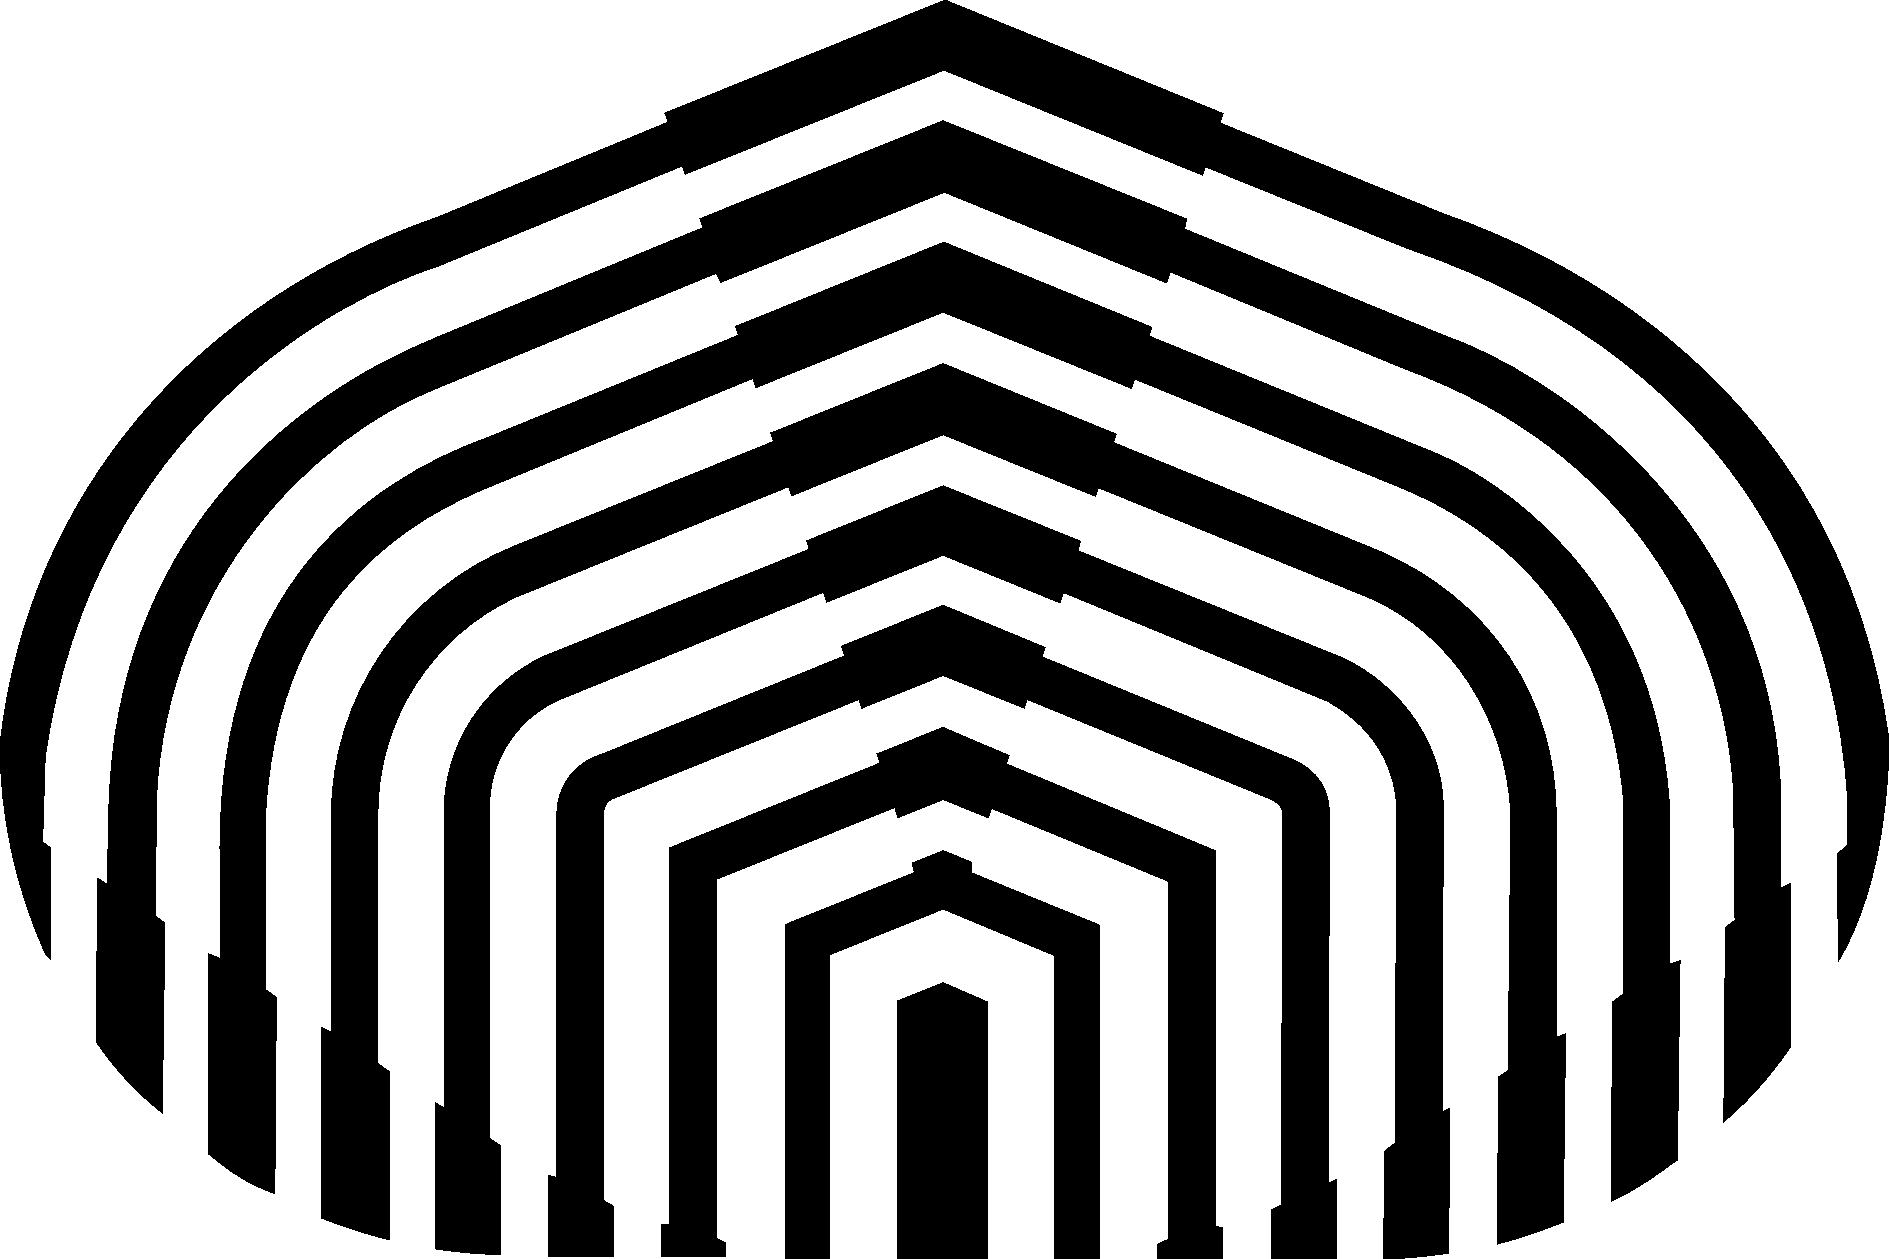
\includegraphics[width=1.2in]{./usb.png} \\[.2cm]
        \large Universidad Simón Bolívar \\
        Decanato de Estudios Profesionales \\
        Coordinación de Ingeniería de Electrónica
        \vfill \LARGE Diseño y Simulación de Procesadores Cuánticos que Implementen Algoritmos Cuánticos de Búsqueda \vfill}
    \author{Por: \\
        Miguel Casanova \\
        Realizado con la asesoría de: \\
        Enrique Castro y Sttiwuer Diaz \\[1.2cm]
        PROYECTO DE GRADO \\
Presentado ante la Ilustre Universidad Simón Bolívar \\
como requisito parcial para optar al título de \\
Ingeniero Electrónico}
    \date{Sartenejas, noviembre de 2018}
\end{titlepage}

\maketitle

\begin{abstract}
El computador cuántico es la promesa tecnológica más relevante del presente siglo, siendo los circuitos cuánticos superconductores los candidatos idóneos para la construcción escalable de procesadores cuánticos eficientes. Un procesador cuántico ejecuta algoritmos cuánticos aplicando secuencias programables de compuertas cuánticas a un registro de entrada conformado por qubits, los cuales evolucionan a un estado cuántico final, el cual es la solución de un algoritmo. Dicho estado cuántico final se caracteriza por tener una familia de correlaciones cuánticas tales como entrelazamiento, discordia cuántica y medida geométrica de la discordia. Experimentalmente, se han logrado implementar en la última década procesadores cuánticos superconductores en base a arquitecturas de transmones, con qubits y qutrits, para los algoritmos cuánticos de Deutsch, Deutsch-Jozsa y Grover. En el presente trabajo se diseñaron y simularon, en base a arquitecturas superconductoras de transmones, procesadores cuánticos que implementen eficientemente los algoritmos cuánticos de Grover y Shor. Además, el internet cuántico permite la comunicación cuántica entre procesadores cuánticos remotos, utilizando procesadores cuánticos locales, que están interconectados por canales de comunicación cuántica que permiten la transmisión de qubits entre los diferentes procesadores, pra resolver problemas que son inviables clásicamente, razón por la cual se estudia la posibilidad de construir circuitos cuánticos del algoritmo de Google Cuántico, así como su representación en una arquitectura superconductora de transmones. En cada uno de los casos estudiados se diseñaron los circuitos cuánticos asociados, su simulación en Python y Mathematica, y se estudió de la información cuántica generada respectivamente.
\end{abstract}


\chapter*{Agradecimientos}

Muchas gracias a Aileen Salas, Alessandra Marrero, Alfredo Ríos, Alfredo Villegas, Álvaro Rodrigues, Andrea Molina, Andrea Ramírez, Andrés Torres, Carlos Castañeda, Carlos Sánchez, Carlota, Carmen Affigne, Carmen Aguilar, Cristhian Da Silva, Daniela Díaz, Daniela González, David Altuve, David Atias, Diosa Medina, Domingo Luis, Domingo Vargas, Eddie Chang, Eder Buitrago, Elinor Appel, Enrique Castro, Enzo D'Argento, Éric Leroux, Elba Guerra, Elba Guerra, Frederick Klindt, Gabriel Marzinotto, Gabriel Mercado, Gabriel Napoli, Gabriel Rodríguez, Gerardo Fernández, Génesis Jiménez, Gilberto Marín, Giancarlo Cuticchia, Gianpaolo Cuticchia, Guillermo Olmos, Guillermo Villegas, Haydn Barros, Héctor Liberatore, Jessica Rondón, Jesús Angarita, Jorge Osorio, José Arcila, Josle Marquina, José Cappelletto, Juan Febles, Juan Pérez, Julio Fuenmayor, Juver Rosillo, Karelia Díaz, Kevin Ng, Kira, Laura Ocanto, Lénore, Lin Song, Lionel Rodríguez, Loinas Barrera, Luis Flores, Luis Anselmi, María Palma, María Jiménez, Mario Quintero, Maurizio Dall'Est, Michelle Márquez, Michelle Woo, Miguel Casanova, Miguel Casanova, Oriana Esparragoza, Pedro Maldonado, Pedro Ovalles, Pedro Pérez, Pelusa, Rafael Silva, Raul Barroso, Roberto Gudiño, Samira Sánchez, Samuel Zambrano, Sara Berman, Silvio Rivero, Stefanni Flores, Steven Leung, Steven Scalzo, Sttiwuer Díaz, Shunichi Watanabe, Valentina Cegarra, Zeigneth Angarita y demás personas que seguro no recuerdo en este momento por su compañía, asistencia, atención, apoyo, tutoría y amistad a lo largo de todos estos años.

\tableofcontents
\listoffigures
%\listoftables

\chapter{Introducción}

La computación cuántica [1-4] está entre las tecnologías más avanzadas, prometedoras y desafiantes del presente siglo. La computación cuántica es un paradigma de computación distinto al de la computación clásica y su objetivo principal es el de controlar la evolución temporal estados cuánticos entrelazados en sistemas multipartitos de alta complejidad. Para ellos se usan qubits, los cuáles son estados cuánticos que pueden estar superpuestos con fases locales relativas complejas, y que además presentan correlaciones cuánticas, que no tienen ningún análogo con aquellas existentes en las arquitecturas existentes para los computadores clásicos, tales como el entrelazamiento, la discordia cuántica, la medida geométrica y la medida geométrica de la discordia.  Un algoritmo cuántico (AC) es un proceso lógico encaminado a realizar una tarea específica. Con frecuencia, las etapas de un AC se pueden concretar en la evaluación de una función sobre distintos parámetros de entrada. El paralelismo cuántico permite a los AC evaluar una función simultáneamente sobre todas las posibles cadenas de n bits. El problema es que la información queda almacenada en las amplitudes de probabilidad del estado cuántico resultante, y para acceder a ella se requiere una medición cuántica, la cual destruye parte de la información. Un AC se representa por un circuito que evoluciona de izquierda a derecha. El estado de entrada suele ser un n-qubit en el estado |0>, y las medidas cuánticas proyectivas fuertes se realizan a la salida del circuito.

Los AC se pueden clasificar en tres clases:

AC Basados en la Transformada Cuántica de Fourier: estos se basan en que podemos formar la serie de Fourier en una superposición de estados cuánticos, y poder operar con ella para obtener los resultados que deseamos. Este tipo de AC es muy importante ya que existen muchos problemas actuales se resuelven a través de la Transformada de Fourier, y una versión cuántica de dicho algoritmo, la cual que provee de un cálculo aún más rápido genera nuevas expectativas tecnológicas.

AC de Búsqueda: Se considera que este tipo de algoritmos es uno de los más importantes ya que muchos problemas tecnológicos pueden reducirse a una búsqueda en bases de datos no estructuradas. Además promete una eficiencia cuadrática en las búsquedas. Uno de los beneficios de utilizar este tipo de algoritmos es que no destruye el conjunto de búsqueda, sino que simplemente marca los valores que satisfacen la condición de búsqueda. Lo cual es muy bueno, ya que al no poderse clonar qubit se garantizaría que los resultados encontrados son únicos.

AC de Simulación: La computación cuántica es la mejor oportunidad tecnológica actual para realizar simulaciones en sistemas cuánticos, y por consiguiente clásicos. En una computadora clásica se necesitan una cantidad exponencial de recursos para poder simular un sistema, sin embargo en una computadora cuántica la cantidad de recursos es lineal. Sin embargo, la eficiencia que se obtiene al simular el sistema no garantiza que se obtenga la información que se desea de la simulación ya que al medir obtenemos una cantidad lineal de datos y no toda la información del sistema. Entonces el reto está en encontrar la manera de encontrar como extraer la información necesaria del sistema sin destruirla. Actualmente esta área del conocimiento está avanzando a ritmos muy acelerados, y la mayoría de los laboratorios de computación cuántica a nivel mundial están logrando grandes avances en este tópico.  Los algoritmos cuánticos están formulados y descritos usando un lenguaje de programación cuántica de alto nivel. Dependiendo de la elección del código de corrección de error cuántico a usar como código de superficie, el compilador toma esa descripción como entrada, realiza la optimización y genera una implementación tolerante a fallas del algoritmo cuántico original. Se necesita una microarquitectura de control para decodificar las instrucciones cuánticas en las señales de control requeridas en tiempos precisos, así como la detección de errores cuánticos en tiempo real y su corrección. Finalmente, basado en la tecnología cuántica específica usada, por ejemplo qubits superconductores, iones atrapados, spin qubits, centros de vacantes de nitrógeno, etc [4], el control las señales se traducen en los impulsos requeridos, y estos se envían al chip a través de una interfaz cuántica-clásica.  En este contexto en el presente trabajo nos vamos a centrar en el estudio de los algoritmos de búsqueda de Grover, de Shor y de Google cuántico.

El AC de búsqueda de Grover resuelve el problema de búsqueda no estructurada en una lista de N datos, con una solución única, usando solamente O(N1/2 ) evaluaciones. En este algoritmo se aprovecha el paralelismo cuántico para evaluar simultáneamente f sobre todos los posibles x de [0,N-1], construyendo, con la transformación de Walsh-Hadamard, y se simula con su circuito cuántico asociado.

La dificultad computacional de resolver el problema de la factorización de enteros es la base del criptosistema RSA. El algoritmo de Shor es un algoritmo cuántico que permite factorizar un número N en tiempos de O(poly(log (N))). Dado N impar y con al menos dos factores primos, el problema de encontrar un factor primo de N se puede reducir al de encontrar el orden de un entero positivo a tal que mcd ( a, N ) = 1. Es decir, se debe encontrar un “t” tal que a mod N . El algoritmo de Shor es polinomial t = 1 respecto al número de dígitos de N. El problema de la factorización se puede reducir al cálculo del período de una función entera, y para ello se puede usar la Transformada Cuántica de Fourier (QFT). Es decir, si f es una función entera y periódica de periodo T, su QFT se anula en todos los elementos del dominio salvo en los múltiplos de la frecuencia w tal que w T = Q.

%F ( |j〉) |wk〉 n ∑ Q−1 j=0 f j = ∑ T−1 k=0 fwk ˆ

%Se aplica la QFT a f y se miden todos los qubits de forma tal que se obtiene wk , tal que 0≤ k ≤ T. Esta propiedad permite obtener la frecuencia, y por tanto el período, de la función f.










En las últimas dos décadas se han desarrollado numerosas plataformas para construir computadores cuánticos (PC). Las más avanzadas hasta ahora se basan en uniones superconductoras de Josephson y en trampas de iones. Particularmente, en el caso de los qubits superconductores [6-8], los más trabajados al día de hoy son los transmones, los cuales son qubits de carga basados en una caja de Cooper derivada capacitivamente de una unión de Josephson, diseñada para tener una sensibilidad reducida a ruidos de carga. Debido a su tamaño microscópico, del orden de micrómetros, los circuitos superconductores se acoplan fuertemente a su entorno en comparación con sistemas microscópicos bien aislados. Aunque esto pudiera parecer un obstáculo aparentemente insuperable, ya se han descubierto y eliminado muchas fuentes de ruido con diseños notablemente inteligentes, y los tiempos de coherencia del qubit se han alargado varios órdenes de magnitud [7] en la última década, haciendo que los sistemas superconductores sean cada vez más la elección más prometedora para el diseño de procesadores cuánticos de múltiples qubits. Actualmente, los procesadores cuánticos se controlan con señales eléctricas bien definidas, por ejemplo, frecuencia de microondas y pulsos, que requieren parámetros y tiempos precisos.

Otras plataformas, bastante prometedoras, que se han comenzado a desarrollar recientemente son los qubits "flip-flop" [9-12], basados en spines electrónicos y nucleares acoplados en sistemas de estado sólido, que permiten acoplamiento de qubits a distancias lo suficientemente largas como para introducir circuitos clásicos de control entre los qubits; y los qubits de modos cero de Majorana, basados en estructuras topológicas de puntos cuánticos y pistas superconductoras sobre sistemas de estado sólido, que son inmunes a errores locales. IBM e Intel, han construido chips de hasta 16 y 17 qubits, respectivamente, utilizando circuitos superconductores. Google e IBM tienen, cada uno, proyectos para construir chips superconductor de 49 qubits para aplicaciones comerciales, entre finales del 2017 y principios del 2018.  En el presente trabajo utilizaremos arquitecturas superconductoras basadas en transmones para el desarrollo y simulación de los AC propuestos. El transmon [12] es una implementación de Uniones Josephson (JJ) basando en cajas de pares de Cooper, que permiten construir compuertas cuánticas que poseen poca decoherencia cuántica. Su nombre es una abreviatura del término qubit de oscilación de plasma derivado de línea de transmisión (transmission line shunted plasma oscillation qubit). En estos los potenciales involucrados permiten construir sistemas de qubit de múltiples niveles, y los niveles más altos son los que a menudo se usan para la implementación de compuertas de 2 qubits. Estos niveles son excitados por microondas. Estos han sido muy eficientes en la implementación de AC como el de Grover [13-16], el de Deutsch–Jozsa [16-18] y el de Shor [19-21].  Recientemente el algoritmo de Grover ha sido estudiado más detenidamente, y se han encontrado nuevas optimizaciones [22], y se también han analizado sus correlaciones cuánticas [23,24]. Similarmente el algoritmo de Shor se ha optimizado recientemente [25, 26], y se han creado circuitos cuánticos mucho más eficientes que los originales, que perfeccionan significativamente la transformada cuántica de Fourier sobre la que se basa dicho algoritmo, hasta el punto que se puede simular en tarjetas FPGA avanzadas [27].

Todo algoritmo cuántico tiene siempre un circuito cuántico asociado. Los primeros algoritmos cuánticos de búsqueda se diseñaron considerando compuertas cuánticas unitarias llamadas oráculos, la cuales eran, matemáticamente hablando, cajas negras que realizaban funciones cuánticas, aunque no se conociera que compuertas cuánticas las conformaban. Sin embargo, es a partir de 2013, con el trabajo de Johnson y colaboradores [28] que la simulación de circuitos cuánticos en computadores clásicos, para obtener los resultados de una búsqueda cuántica, han adquirido capital importancia. La idea de no simular dichos circuitos cuánticos, sino de implementarlos físicamente ya es un hecho para empresas como IBM, NCIT, GOOGLE e INTEL. Recién en el 2016, La empresa IBM publicó en Internet una página web de acceso libre, en la cual si se deseaba simular un circuito cuántico sólo debía escribirlo sobre una plataforma específica, y ella lo simulaba y daba los resultados solicitados, en tiempos muy breves, los cuales mostraban de manera diáfana la ventaja del computador cuántico sobre el clásico.. Aún más, ellos ofrecían la posibilidad de lograr la realización experimental de dicho circuito, para un número finito de qubits con solo solicitárselo a dicha empresa. IBM implementaba el circuito en arquitecturas de transmones, y daba los resultados. Esta oportunidad única para los investigadores del área tenía solo dos limitantes: (1) nadie sabía cuál era la tecnología que ellos usaban, y (2) era una versión beta que se ofrecía públicamente para que las masas de investigadores en el mundo al usarlas ayudaran a la IBM a que por ensayo y error pudieran detectar sus errores de diseño. Ya a mediados de este año se puso como norma de la empresa que quien deseara usar esos beneficios tecnológicos debería pagar, comercializando así el uso de dicha herramienta.

Siguiendo en el contexto de desarrollar PC acordes a las realidades comerciales y de investigación, ya se han desarrollado circuitos cuánticos completamente tolerantes a errores cuánticos [29], permitiendo así crear circuitos cuánticos de alto nivel de precisión. Sin embargo, los métodos de control existentes introducen un alto consumo de recursos, largos tiempos de configuración y de complejidad de control. Por esta razón, el diseño de procesadores cuánticos capaces de implementar algoritmos cuánticos con funciones especificas, de forma eficiente y que minimicen los recursos de control es una de los retos más grandes para los Ingenieros Electrónicos en el área de Estado Sólido y de los Físicos.  Por otro lado, El desarrollo de las tecnologías superconductoras ha logrado que algunos algoritmos que existían solo en el mundo teórico de la computación cuántica tales como el algoritmo para resolver sistemas de ecuaciones lineales [30], se hayan logrado implementar experimentalmente en el 2017 [31], obteniendo resultados precisos que tienen muy alta fidelidad.

Una de las aplicaciones más importantes para la navegación en las Redes de Comunicación Cuántica que actualmente se están desarrollando en Europa, Asia y Estados Unidos, es el algoritmo de Google Cuántico [32]. Su implementación experimental [33] ha ilustrado la importancia del mismo para cuantificar las cadenas de Markov dentro de la matriz del algoritmo de busque de Google. En este trabajo, se desea Diseñar y simular PC que implementen los algoritmos cuánticos de Grover, Shor y Google Cuántico, en base a arquitecturas superconductoras de transmones y con énfasis en incorporar las innovaciones más modernas que hay para los algoritmos de Grover y Shor.  Por otro lado, el algoritmo de Google Cuántico, hasta donde sabemos, no posee ningún circuito cuántico asociado. Por esta razón se desea construir un circuito que resuelva los sistemas lineales que conlleva la matriz del grafo cuántico del algoritmo de Google Cuántico y optimizar el proceso de búsqueda dentro de la red cuántica asociada.

Se obtendrán todas las codificaciones cuánticas de cada uno de los PC a desarrollar usando el software Mathematica, y se realizaran las simulaciones numéricas en Python. Se analizaran las correlaciones cuánticas en cada uno de los casos considerados, con el interés de entender cómo se comporta la información cuántica generada, y como esta cambia una vez se han realizado las medidas cuánticas fuertes respectivas, buscando así determinar qué criterios de medida y de control se han de seguir al medir la información generada por dichos PC 

\section{JUSTIFICACION}

La Computación Cuántica y la Comunicación Cuántica son dos áreas tecnológicas que apenas teniendo dos décadas de desarrollo, ofrecen resultados muy prometedores. En particular los últimos dos años marcan una diferencia histórica en el área, diferencia que ya promete que en menos de 5 años se comercializaran muchísimas aplicaciones novedosas que afectaran las culturas tecnológicas de las sociedades mundiales futuras. En mayo de 2016, la Comunidad Europea llego a un acuerdo conocido como el “Quantum Manifesto” [34], en el cual todos los países miembros se comprometían a aportar entre todos el monto de 1 billón de euros, el cual se usará para lograr que toda Europa en el 2035 tenga la totalidad de sus tecnologías basadas en plataformas cuánticas, desde el ordenador cuántico más simple usado por el ciudadano común, hasta la totalidad de las redes de comunicación. Se prevé el desarrollo aplicaciones en todas las áreas del conocimiento humano con un desarrollo imperativo en las tecnologías militares, medicina, energía alternativas, etc.

Actualmente, el “Quantum Manifesto”, ha servido como motivación para que los países del primer mundo traten de crear una red cuántica de comunicación global en el planeta [35]. Es importante entender que cuando estas tecnologías se desarrollen se podrán construir computadores cuánticos universales capaces de resolver problemas que a un supercomputador actual le tomaría más tiempo que la edad actual del universo, lo que significa para la raza humana un cambio total en su evolución tecnológica creando nuevos paradigmas en la interpretación del Universo.

En este año 2017, el número de avances logrados en investigación básica y con grandes oportunidades de aplicación comercial ha sido muy amplio, entre las cuales podemos citar:
1) La creación del primer cheque cuántico con un PC de 5 qubits [36].
2) El diseño de circuitos clásicos que simulan el algoritmo de Shor [37].
3) El desarrollo de tecnologías cuánticas para el procesamiento de cuánticos imágenes y de películas, las cuales
permitirían realizar el procesado de estas con fidelidades muy superiores a las de HD actuales, usando para ello
algoritmos cuánticos asistidos por PC [38].
4) El desarrollo de sistemas de distribución de llaves cuánticas (QKD) en criptografía cuántica, basados en procesos
de aprendizaje cuántico (quantum maching learning) [39]. Actualmente en los países del primer mundo se desean
construir PC que tengan QKD con aprendizaje cuántico.
5) La posibilidad de construir PC nanométricos muy eficientes, y resistentes, con diamantes artificiales excitados
con nanofotónica [40]
6) La creación de redes cuánticas de comunicación satelital que permiten distribuir entrelazamiento a 1200 Km de
distancia, por nanosatélites [41]. Estas ampliaciones están en este momento en desarrollo experimental-militar, y el
gobierno chino ha informado que van a comercializarse a partir del 2018.
7) El desarrollo de algoritmos y circuitos cuánticos capaces de simular eficientemente las redes neurales, logrando
por primera vez reproducir los comportamientos reales de dichas redes basándose en la distribución del
entrenamiento cuántico [42]. Este resultado es muy importante ya que al desarrollar PC capaces de reproducir estas
redes podríamos realizar inimaginables avances en el entendimiento del cerebro humano, y del estudio de la
inteligencia artificial cuántica.

Como podemos observar el cambio tecnológico que se avecina, puede colocar a muchos países en profundas desventajas con otros. Solo aquellos que tengan acceso y entiendan estas nuevas tecnologías podrán ir al ritmo del desarrollo de las mismas, y aquellos que no lo hagan tendrán solo dos opciones: o las compran (creando así una profunda dependencia), o se quedan en un total atraso tecnológico.

Es por esta razón que se propone el presente trabajo de grado. En Venezuela no existe actualmente ningún desarrollo de tecnologías cuánticas, ni en Ingeniería Electrónica, ni en la Física aplicada. Por otro lado, debido a la realidad país actual, es imposible crear ningún PC, ni superconductor ni en base a tecnologías de silicón, diamante, puntos cuánticos, trampa de iones, átomos neutros, etc [4]. Sin embargo, si poseemos el nivel teórico para diseñar y simular arquitecturas superconductoras basadas en transmones, de PC que puedan realizar funciones específicas de aplicación directa tanto comerciales como de investigación básica.  Este trabajo sería pionero en Venezuela, y los logros obtenidos motivarán a la Universidad Simón Bolívar para continuar realizando otros trabajos de grado (Pregrado, Maestría y Doctorado), capaces de generar temas de

investigación, e implementar aplicaciones industriales que permitan en un futuro no lejano alcanzar una masa crítica de Ingenieros y Físicos capaces de permitir la actualización e inclusión del país en estas nuevas tecnologías de frontera.

\section{OBJETIVOS}

\subsection{Objetivo General:}

Diseñar y simular PC que implementen los AC de Grover, Shor y Google Cuántico.

\subsection{Objetivos Específicos:}

1) Construir la representación circuital cuántica de los AC de Grover, Shor y de Google Cuántico.
2) Diseñar arquitecturas superconductoras controlables por microondas basadas en transmones.
3) Hallar las respectivas secuencias de pulsos, que son necesarios para generar con transmones la
representación circuital cuántica de los tres AC considerados.
4) Simular en Mathematica, en forma algebraica, cada una de las arquitecturas de CC consideradas,
permitiendo así obtener expresiones lo mas simplificadas posibles de los procesos cuánticos considerados.
5) Simular en Python, de forma numérica, el operador evolución de cada una de los compuertas de los CC
estudiados, y generalizar dicha simulación a cada una de las arquitecturas superconductoras.
6) Analizar los resultados obtenidos, mostrando que ventajas ofrecen las mejoras consideradas en el
diseño de los CC creados para cada uno de los AC estudiados en el presente trabajo.

\subsection{Fases del Proyecto}

1) Estudiar la electrónica de estado sólido que contienen las Uniones Josephson, y cómo se construyen los
Transmones a partir de estas. (EP-1206)
2) Hacer una revisión bibliográfica detallada, de todas las publicaciones existentes hasta la fecha, de los
AC de Grover, Shor y de Google Cuántico. (EP-1206)
3) Estudiar detalladamente la Mecánica Cuántica que permite crear cada uno de estos AC. (EP-1206)

4) Construir la representación circuital cuántica de cada uno de dichos AC. (EP-2206)
5) Hallar las arquitecturas superconductores, y las respectivas secuencias de pulsos, que son necesarios
para generar con transmones la representación circuital cuántica de los tres AC considerados. (EP-2206)
6) Simular en Mathematica, en forma algebraica, cada una de las arquitecturas de CC consideradas,
permitiendo así obtener expresiones lo mas simplificadas posibles de los procesos cuánticos considerados.
(EP-2206)
6) Simular en Python, de forma numérica, el operador evolución de cada una de los compuertas de los CC
estudiados, y generalizar dicha simulación a cada una de las arquitecturas superconductoras. (EP-2206)
7) Analizar los resultados obtenidos, mostrando que ventajas ofrecen las mejoras consideradas en el
diseño de los CC creados para cada uno de los AC estudiados en el presente trabajo. (EP-3206)





\subsection{REFERENCIAS}

1.- M. Hayashi, S. Ishizaka, A. Kawachi, G. Kimura and T. Ogawa, “Introduction to Quantum Information Science”, Springer-Verlag Berlin Heidelberg (2015)
2.- J. A. Jones and D. Jaksch, “Quantum Information, Computation and Communication”, Cambridge University Press (2012)
3.- M.A. Nielsen, I.L. Chuang, “Quantum Computation and Quantum Information”, Cambridge University Press (2011)
4.- M. Nakahara and T. Ohmi , “Quantum computing : from linear algebra to physical realizations “CRC Press, Taylor and Francis Group (2008)
5.- R. J. Lipton and K. W. Regan, “Quantum Algorithms via Linear Algebra: A Primer”, MIT Press books (2014)
6.- G. Wendin, “Quantum information processing with superconducting circuits: a review”, Rep. Prog.  Phys. 80, 106001 (2017)
7.- M. H. Devoret and R. J. Schoelkopf , “Superconducting Circuits for Quantum Information: An Outlook”, Science 339, 1169 (2013)
8.- Y. Hu, Y. X. Zhao, Z.-Y. Xue and Z. D. Wang, “Realizing universal quantum gates with topological bases in quantum-simulated superconducting chains”, npj Quantum Information 3, 8 (2017)
9.- D.Rotta, F. Sebastiano, E. Charbon and E. Prati, “Quantum information density scaling and qubit operation time constraints of CMOS silicon-based quantum computer architectures”, npj Quantum Information 3, 26 (2017)
10.- G. Tosi, F. A. Mohiyaddin, V. Schmitt et al. , “Silicon quantum processor with robust long-distance qubit couplings”, Nature Communications 8, 450 (2017)
11.- N. Harris, D. Bunandar, M. Pant, et al., “Large-scale quantum photonic circuits in silicon”, Nanophotonics, 5, 456-468 (2016)
12.- Koch J et al., “Charge insensitive qubit design from optimizing the cooper-pair box”, Phys. Rev. A 76, 042319 (2007)
13.- L. K. Grover, “A fast quantum mechanical algorithm for database search”, Phys. Rev. Lett. 79, 325 (1997)

14.-A. Dewes, R. Lauro, F. R. Ong, et al., “Quantum speeding-up of computation demonstrated in a superconducting two-qubit processor”, Phys. Rev. B 85, 140503(R) (2012)
15.- T. Said, A. Chouikh, K. Essammouni and M. Bennai, “Implementation of Grover quantum search algorithm with two transmon qubits via circuit QED”, Quant. Phys. Lett. 6, 29-35 (2017)
16.- L. DiCarlo, J. M. Chow, J. M. Gambetta, “Demonstration of two-qubit algorithms with a superconducting quantum processor”, Nature 460, 240-244 (2009)
17.- D. Deutsch and R. Jozsa, "Rapid solutions of problems by quantum computation", Proceedings of the Royal Society of London A. 439, 553 (1992)
18.- J. Zhao, X. Tan, D. Lan et al., “Implementation of refined Deutsch–Jozsa algorithm in a superconducting qutrit system”, Phys. Status Solidi B, 1–5 (2016)
19.- P. W. Shor, “Polynomial-Time Algorithms for Prime Factorization and Discrete Logarithms on a Quantum Computer”, SIAM J. Comput. 26, 1484 (1997)
20.- J. M. Gambetta, J.M. Chow and M. Steffen, “Building logical qubits in a superconducting quantum computing system”, npj Quantum Information 3, 2 (2017)
21.- T. Monz, D. Nigg, E. A. et al., “Realization of a scalable Shor algorithm”, Science 351, 1068-1070 (2016)
22.- I. Chakrabarty, S. Khan, and V. Singh, “Dynamic Grover search: applications in recommendation systems and optimization problems”, Quantum Inf. Process. 16, 153 (2017)
23.- K. V. Gubaidullina and S A Chivilikhin, “Theoretical research of the distortion of quantum circuit in Grover's algorithm”, Journal of Physics Conference Series 735, 012074 (2016)
24.- B. Ye, T. Zhang, L. Qiu and X. Wang, “Quantum discord and entanglement in grover search algorithm”,Open Physics 14, 171–176 (2016)
25.- R. Dridi and H. Alghassi, “Prime factorization using quantum annealing and computational algebraic geometry”, Sci. Rep. 7, 43048 (2017)
26.- N. Johansson and J.-A. Larsson, “Realization of Shor’s Algorithm at Room Temperature”, arXiv:1706.03215v1 (10 Jun 2017)
27.- Y. H. Lee, M. Khalil-Hani, and M. N. Marsono, “An FPGA-Based Quantum Computing Emulation Framework Based on Serial-Parallel Architecture”, International Journal of Reconfigurable Computing 2016, 5718124 (2016)
28.- T. H. Johnson J. D. Biamonte S. R. Clark and D. Jaksch , “ Solving search problems by strongly simulating quantum circuits”, Sci Rep. 3, 1235 (2013)
29.- A. Paler, I. Polian, K. Nemoto and S. J Devitt, “Fault-tolerant, high-level quantum circuits: form, compilation and description”, Quantum Sci. Technol. 2, 025003 (2017)

30.- Y. Caoa, A. Daskinb, S. Frankela and S. Kais, “Quantum circuit design for solving linear systems ofequations”, Molecular Physics 110, 1675–1680 (2012)
31.- Y. Zheng, C. Song, M.-C. Chen, et al. “Solving Systems of Linear Equations with a Superconducting Quantum Processor”, Phys. Rev. Lett. 118, 210504 (2017)
32.- G.D. Paparo, M. Müller, F. Comellas, et al. ,“Quantum Google algorithm”, Eur. Phys. J. Plus 129, 150 (2014)
33.- J. A. Izaac, X. Zhan, Z. Bian, K. Wang, J. Li, J. B. Wang, and P. Xue, “Centrality measure based on continuous-time quantum walks and experimental realization”, Phys. Rev. A 95, 032318 (2017)
%34.- https://msu.euramet.org/current_calls/fundamental_2017/documents/Quantum_Manifesto.pdf
35.- Christoph Simon, “Towards a global quantum network”, Nature Photonics 11, 678–680 (2017)
36.- B. K. Behera, A. Banerjee and P. K. Panigrahi, “Experimental realization of quantum cheque using a five-qubit quantum computer”, Quantum Inf. Process. 16, 312 (2017)
37.- N. Johansson and J.-A. Larsson, “Realization of Shor’s Algorithm at Room Temperature”, arXiv:1706.03215v1 (10 Jun 2017)
38.- Fei Yan, Abdullah M. Iliyasu, Phuc Q. Le, “Quantum image processing: A review of advances in its security technologies”, Int. J. Quantum Inf. 15 , 1730001 (2017)
39.- B. Shenga and L. Zhoub, “Distributed secure quantum machine learning”, Science Bulletin 62, 1025-1029 (2017)
40.- J. L. Zhang, K. G. Lagoudakis, Y.-K. Tzeng, et al. “Complete coherent control of silicon vacancies in diamond nanopillars containing single defect centers”, Optica 4, 1317-1321 (2017)
41.- D.-L. Deng, X. Li, and S. Das Sarma, “Quantum Entanglement in Neural Network States”, Phys.  Rev. X 7, 021021 (2017)
42.- J. Chen, L. Wang and E. Charbon, “A quantum-implementable neural network model”, Quantum Inf. Process. 16, 245 (2017)

\chapter{Información cuántica}

En esta sección introduciremos las bases matemáticas fundamentales para empezar a trabajar con la Teoría de Información Cuántica, trabajaremos sobre espacios vectoriales discretos, debido a que los sistemas cuánticos que manejaremos (computadora cuántica) son sistemas físicos discretos, no continuos. Se dará una breve introducción a la notación de Dirac y su aplicación en la mecánica cuántica. Una vez establecidas las bases matemáticas se describirán los Postulados de la Mecánica Cuántica: Descripción del estado de un sistema, descripción de cantidades físicas, medición de cantidades físicas, reducción del paquete de ondas, evolución temporal, postulado de simetrización y variables de espín. Finalmente se definirá el enredamiento cuántico, su importancia en el cómputo cuántico y los sistemas de dos niveles.

\section{Función de onda}

El estado de una sistema cuántico viene dado por el conocimiento de un campo escalar denominado función de onda $\psi$ en todos los puntos del espacio para cualqueir instante de teimpo, dicha función de onda es compleja ($\in \mathds{C}$), de cuadrado integrable, cumple con el principio de superposición y es univaluada para las coordenadas espaciales de cada una de las partículas. Conocer la función de onda en mecánica cuántica es equivalente a conocer los vectores posición y momentum en mecánica clásica, en el sentido de que esta es la condición suficiente y necesaria para conocer el sistema en su totalidad. La evolución de la función de onda está dada por la ecuación de Schrödinger. La mecánica cuántica es una teoría probabilística, una partícula puede encontrarse en cualquier parte del universo en cualquier momento y la densidad de probabilidad de encontrarla en algún punto está dada por el módulo al cuadraro de su función de onda en este punto. De hecho, debido a esto es que $\psi$ debe ser de cuadrado integrable, pues la probabilidad de que la partícula se encuentre en cualquier lugar del universo debe ser uno, es decir:

\begin{equation}
    \int\limits_S \abs{\psi(r,t)}^2 dr = 1
\end{equation}

Donde $S$ es todo el universo. Esto es para funciones de onda que describen una partícula, en el siguiente capítulo se verán funciones de onda macroscópicas que describen sistemas de muchas partículas. En estos, el módulo cuadrádo de $\psi$ describe la densidad de partículas, la cual podría entenderse como la suma de la densidad de probabilidad de que cada una de las partículas se encuentren en ese punto, y $\int\limits_S \abs{\psi(r,t)}^2 dr = N_s$, donde $N_s$ es el número total de partículas del sistema, el cual podría entenderse como la suma de que cada una de las partículas se encuentre en algún punto del sistema.

%Según la mecánica clásica, ondas y partículas son dos entidades distintas, la primera es un ente puntual con posición definida que transporta masa, momentum y energía por el espacio, mientras que una onda es un ente disperso que transporta momentum y energía, pero no masa. En la mecánica cuántica existe la dualidad partícula-onda. Los entes cuánticos nos son partículas u ondas como se entienden en la mecánica clásica, pero se pueden comportar como estos bajo ciertas condiciones. Por ejemplo, un electrón que se dispara por un cañón tendrá una probabilidad de encontrarse en cierta región del espacio, pero a diferencia de la mecánica estadística clásica, este electrón no es una partícula cuya posición exacta se desconoce, sino que tiene comportamientos propios de una onda, como la interferencia destructiva. Este comportamiento de onda se mantiene hasta que se realice una medida de la posición de este electrón. En ese momento, la distribución de probabilidad de la posición de ese electrón se concentra en un punto y pasa a comportarse como una partícula. Lo mismo sucede con los fotones, que son las partículas de la luz. De hecho, debido a la naturaleza cuántica de la luz es que existen fenómenos como el efecto fotoeléctrico, el cual es un fenómeno de partículas, a pesar de que clásicamente la luz sea una onda.

%Es importante resaltar que a pesar de que los objetos cuánticos se puedan comportar como partículas u ondas clásicas bajo ciertas condiciones, en ningún momento son ondas ni partículas como se entiende en la mecánica clásica. Por ejemplo, la ``onda electrónica'' del párrafo anterior es una ``onda'' que transporta masa, mientras que en la definición de onda se especifíca explícitamente que las ondas no transportan masa. Por otro lado, los fotones son partículas sin masa, lo cual también es algo que no sucede con las partículas de la mecánica clásica. Así que los objetos cuánticos, a pesar de que lleven el nombre de "partícula" y se hable de la dualidad onda-partícula, no son ondas, ni partículas. Sólo son objetos cuyas propiedades vienen descritas por una función compleja de cuadrado integrable, cuyo módulo al cuadrado está asociado a una densidad de probabilidad.

\section{Espacio de Hilbert}

Los espacios de Hilbert, creados por el matemático David Hilbert y normalizados por John von Neumann en el siglo XX, son el soporte matemático de la mecánica cuántica. Un espacio de Hilbert es un espacio vectorial complejo $\mathcal{H}$ de cuadrados integrables con un producto interno $(f,g)$ donde la norma vectorial se define como $\norm{f} = \sqrt{(f,f)}$.

Un conjunto de $2^n$ funciones $B = \{f_n\} \subset \mathcal{H}$ es llamado base ortonormal de $\mathcal{H}$ si y sólo si:

\begin{align}
    (f_n, f_m) &= \delta_{n } \quad \forall f_n, f_m \in B
\end{align}

Todo elemento $\psi \in \mathcal{H}$ puede ser escrito como:

\begin{equation}
    \psi = \sum\limits_n c_n \psi_n
\end{equation}

En la mecánica cuántica, todas las funciones de onda deben pertenecer un espacio de Hilbert normalizado. Es decir, pertenecen al espacio de Hilbert donde:

\begin{equation}
    \norm{\psi} = 1 \quad \forall \psi \in \mathcal{H}
\end{equation}

Los espacios de Hilbert tienen las siguientes propiedades:

\begin{enumerate}
    \item Producto escalar: $(\psi, \phi) = \int\limits_S \psi^* \phi dr \quad \in \mathds{C}$
    \item Simetría $(\psi, \phi) = (\phi, \psi)^*$
    \item Linealidad: $(\psi, \alpha \phi_1 + \beta \phi_2) = \alpha (\psi, \phi_1) + \beta (\psi, \phi_2)$
    \item Antilinealidad: $(\alpha \psi_1 + \beta \psi_2, \phi) = \alpha^* (\psi_1, \phi) + \beta^* (\psi_2, \phi)$
    \item Ortogonalidad: $(f_i, f_j) = 0$
    \item Autoproducto escalar: $(\psi, \psi) \neq 0$ ($(\psi, \psi) = 1$ si y sólo si $\psi$ está normalizada)
    \item Norma: $\norm{\psi} = \sqrt{(\psi,\psi)}$
    \item Desigualdad de Cauchy: $\norm{(\psi_1,\psi_2)} \leq \sqrt{(\psi_1,\psi_1)} \sqrt{(\psi_2,\psi_2)}$
    \item Operadoers lineales: $\psi^\prime = \hat{A} \psi$
\end{enumerate}

\section{Delta de Kronecker}

La delta de Kronecker, $\delta_{n,m}$ es un símbolo que representa dos posibles valores, dependiendo de sus índices,

\begin{equation}
    \delta_{n,m} =
    \begin{cases}
        1, & n = m \\
        0, & n \neq m
    \end{cases}
\end{equation}

Dado que el símbolo sólo es diferente de cero cuando sus índices son iguales, las sumas que incluyen la delta de Kronecker pueden ser simplificadas fácilmente

\begin{equation*}
    \sum\limits_m \delta_{nm} B_m = 0 B_1 + 0 B_2 + ... + 1 B_n + ... = B_n
\end{equation*}

\section{Operadores hermíticos}

Estos son operadores tales que $U = U^\dagger$, donde $U^\dagger = (U^*)^T$. Es decir, U es un operador hermítico si es igual a su transpuesto conjugado. Estos operadores cumplen con la propiedad de que todos sus autovalores son reales. En la mecácina cuántica, todas las variables físicas observables (o simplemente, observables), es decir, todas aquellas variables que se pueden medir en un laboratorio, son autovalores asociados a un operador hermítico.

\section{Operadores unitarios}

Estos son operadores tales que $U U^\dagger = \mathds{1}$ con determinante igual a 1. En la mecánica cuántica todas las operaciones que se realicen sobre o que afecten a un un estado y no involucren medidas ni decoherencia tienen un operador unitario asociado. Por ejemplo, la evolución temporal tiene un estado unitario $U$ asociado. Los operadores unitarios son importantes porque ellos preservan las trazas, las normas y la información, de esta manera, cuando se aplica un operador unitario a un estado cuántico, se preserva la normalización de las probabilidades y el entrelazamiento.

\section{Notación de Dirac}

En 1930 en el libro Principios de la Mecánica Cuántica Paul Dirac introdujo una poderosa notación para poder describir estados cuánticos y funciones lineales, también conocida como notación Bra-Ket. Con la notación de Dirac podemos representar un estado base de $n$ elementos con una cadena binaria de longitud $n$, mientras que con la representación de vectores columna necesitariamos $2^n$ componentes para definir el mismo vector.

La notación bra-ket es la notación estándar en la mecánica cuántica para describir estados cuánticos. En el caso de la computación cuántica, se utilizan los kets $\ket{0}$ y $\ket{1}$ para describir los qubits en la base computacional. Este par de estados sería el equivalente a los bits 0 y 1 en la computación clásica. En su representación matricial, los kets $\ket{0}$ y $\ket{1}$ se representan de la siguiente manera:

\[\ket{0} = \begin{pmatrix} 1 \\ 0 \end{pmatrix}\]

\[\ket{1} = \begin{pmatrix} 0 \\ 1 \end{pmatrix}\]

Un bra es el operador adjunto de un ket. Los bras de la base computacional son $\bra{0}$ y $\bra{1}$. En la representación matricial estos son la transpuesta conjugada de los kets y se representan de la siguiente manera:

\[\bra{0} = \begin{pmatrix} 1 & 0 \end{pmatrix}\]

\[\bra{1} = \begin{pmatrix} 0 & 1 \end{pmatrix}\]

El producto interno de kets es el producto de un bra seguido de un ket $\braket{\phi}{\psi}$, el resultado de este producto es un número complejo y cumple las siguientes propiedades:

\begin{align}
    \braket{\phi}{\psi} &= z \\
    (\braket{\phi}{\psi})^\dagger &= \braket{\psi}{\phi} = z^*
\end{align}

El producto externo es el producto de un ket seguido de un bra $ketbra{\phi}{\psi}$. El resultado es un proyector que toma la componente en $\ket{\psi}$ de un estado cuántico y la convierte en $\ket{\phi}$. Ejemplos:

\begin{align*}
    \ketbra{0}{0} &= \begin{pmatrix} 1 \\ 0 \end{pmatrix} \begin{pmatrix} 1 & 0 \end{pmatrix} = \begin{pmatrix} 1 & 0 \\ 0 & 0 \end{pmatrix} \\
    \ketbra{0}{1} &= \begin{pmatrix} 1 \\ 0 \end{pmatrix} \begin{pmatrix} 0 & 1 \end{pmatrix} = \begin{pmatrix} 0 & 1 \\ 0 & 0 \end{pmatrix} \\
    \ketbra{1}{0} &= \begin{pmatrix} 0 \\ 1 \end{pmatrix} \begin{pmatrix} 1 & 0 \end{pmatrix} = \begin{pmatrix} 0 & 0 \\ 1 & 0 \end{pmatrix} \\
    \ketbra{1}{1} &= \begin{pmatrix} 0 \\ 1 \end{pmatrix} \begin{pmatrix} 0 & 1 \end{pmatrix} = \begin{pmatrix} 0 & 0 \\ 0 & 1 \end{pmatrix} \\
    \ketbra{\psi}{\psi} &= (\alpha \ket{0} + \beta \ket{1})(\alpha^* \bra{0} + \beta^* \bra{1}) = \begin{pmatrix} \abs{\alpha}^2 & \alpha \beta^* \\ \alpha^* \beta & \abs{\beta}^2 \end{pmatrix}
\end{align*}

Este producto cumple con las siguientes propiedades:

\begin{align}
    \ketbra{\phi}{\psi} &= \Pi \\
    (\ketbra{\phi}{\psi})^\dagger &= \ketbra{\psi}{\phi} = \Pi^\dagger
\end{align}

El operador $\Pi$ que consiste de un producto exterior se conoce como proyector. La aplicación de un proyector $\ketbra{\psi}{\phi}$ sobre un estado $\ket{\varphi}$ es equivalente a la multiplicación del escalar $c = \braket{\phi}{\varphi}$ al estado $\psi$.

\begin{equation}
    \ketbra{\psi}{\phi} \ket{\varphi} = \braket{\phi}{\varphi} \ket{\psi} = c \ket{\psi}
\end{equation}

Si además, el proyector es tal que $\ket{\psi} = \bra{\phi}^\dagger$, es decir: $\Pi = \ketbra{\psi}{\psi}$, entonces se cumple también que:

\begin{align}
    \Pi^2 &= \ketbra{\psi}{\psi} \ketbra{\psi}{\psi} = 1 \ketbra{\psi}{\psi} = \Pi \\
    \Pi^\dagger &= (\ketbra{\psi}{\psi})^\dagger = \ketbra{\psi}{\psi} = \Pi
\end{align}

La notación de Dirac se relaciona con el formalismo de funciones de onda de la siguiente manera:

\begin{equation}
    \psi = \braket{x}{\psi}
\end{equation}

Donde $\bra{x}$ es el bra asociado a estar en la posición $x$.

\section{Producto tensorial}

Cuando un sistema compuesto por dos (o más) espacios de Hilbert, $\mathcal{H}_A$ y $\mathcal{H}_B$, el espacio del sistema completo se escribe en función del producto tensorial $\mathcal{H} = \mathcal{H}_A \otimes \mathcal{H}_B$. Aquí, $\mathcal{H}_A$ y $\mathcal{H}_B$ se conocen como las particiones de $\mathcal{H}$. De igual manera, para representar un estado de $\mathcal{H}$ en un ket, en lugar de dos, se realiza el producto tensorial $\ket{\psi} = \ket{\psi_1} \otimes \ket{\psi_2}$. También se pueden agregar subindices a los kets para hacer énfasis en las particiones:

\begin{array}{c c}
    $\ket{\psi}$ & $\in \mathcal{H}$ \\
    $\ket{\psi}_A \otimes \ket{\phi}_B$ & $\in \mathcal{H}_A \otimes \mathcal{H}_B$ \\
    $\ket{\psi_1}_1 \otimes \ket{\psi_2}_2 \otimes ... \otimes \ket{\psi_n}_n$ & $\in \mathcal{H}_1 \otimes \mathcal{H}_2 \otimes ... \otimes \mathcal{H}_n$
\end{array}

En la representación matricial el producto tensorial se realiza de la siguiente manera:

\begin{equation*}
    \ket{\psi_1} \otimes \ket{\psi_2} =
    \begin{pmatrix}
        a \\
        b
    \end{pmatrix}
    \otimes
    \begin{pmatrix}
        c \\
        d
    \end{pmatrix}
    =
    \left(\!\!\!\begin{array}{c}
            a \left(\!\!\begin{array}{c}
                    c \\
                    d \\
            \end{array}\!\!\right) \\
            b \left(\!\!\begin{array}{c}
                    c \\
                    d \\
            \end{array}\!\!\right)
    \end{array}\!\!\!\right)
    =
    \begin{pmatrix}
        a c \\
        a d \\
        b c \\
        b d \\
    \end{pmatrix}
\end{equation*}

El producto tensorial tiene las siguientes propiedades:

\begin{align}
    (U_1 \otimes U_2) (\ket{\psi_1} \otimes \ket{\psi_2}) &= (U_1 \ket{\psi_1}) \otimes (U_2 \ket{\psi_2}) \\
    \ket{\psi_1} \otimes \ket{\psi_2} &\neq \ket{\psi_2} \otimes \ket{\psi_1} \\
    \alpha (\ket{\psi_1} \otimes \ket{\psi_2}) &= (\alpha \ket{\psi_1}) \otimes \ket{\psi_2} = \ket{\psi_1} \otimes (\alpha \ket{\psi_2}) \\
    (\ket{\psi_1} \otimes \ket{\psi_2})^\dagger &= \bra{\psi_1} \otimes \bra{\psi_2}
\end{align}

En el caso de los bras y los kets, el producto tensorial también se puede escribir de la forma $\ket{\psi\phi}$, en lugar de $\ket{\psi} \otimes \ket{\phi}$.

%Un estado multipartito se puede escribir de la forma extensa $\ket{\psi} \otimes \ket{\phi}$ o de la forma compacta $\ket{\psi \phi}$. También se pueden agregar subíndices para hacer énfasis en las particiones $\ket{\psi}_A \otimes \ket{\phi}$. Entonces:

\begin{equation*}
    \ket{\psi}_A \otimes \ket{\phi}_B = \ket{\psi} \otimes \ket{\phi} = \ket{\psi_A \phi_B} = \ket{\psi\phi}
\end{equation*}

Ejemplos:

\begin{equation*}
    \ket{0} \otimes \ket{0}
    = \begin{pmatrix} 1\\0 \end{pmatrix} \otimes \begin{pmatrix} 1\\0 \end{pmatrix}
    = \begin{pmatrix} 1\\0\\0\\0 \end{pmatrix}
\end{equation*}

\begin{equation*}
    \ket{0} \otimes \ket{1}
    = \begin{pmatrix} 1\\0 \end{pmatrix} \otimes \begin{pmatrix} 0\\1 \end{pmatrix}
    = \begin{pmatrix} 0\\1\\0\\0 \end{pmatrix}
\end{equation*}

\begin{equation*}
    \ket{1} \otimes \ket{0}
    = \begin{pmatrix} 0\\1 \end{pmatrix} \otimes \begin{pmatrix} 1\\0 \end{pmatrix}
    = \begin{pmatrix} 0\\0\\1\\0 \end{pmatrix}
\end{equation*}

\begin{equation*}
    \ket{1} \otimes \ket{1}
    = \begin{pmatrix} 0\\1 \end{pmatrix} \otimes \begin{pmatrix} 0\\1 \end{pmatrix}
    = \begin{pmatrix} 0\\0\\0\\1 \end{pmatrix}
\end{equation*}

\begin{equation*}
    \mathds{1} \otimes \sigma_x
    = \begin{pmatrix}
        1 & 0 \\
        0 & 1
        \end{pmatrix} \otimes
        \begin{pmatrix}
            0 & 1 \\
            1 & 0
        \end{pmatrix}
    = \begin{pmatrix}
        0 & 1 & 0 & 0 \\
        1 & 0 & 0 & 0 \\
        0 & 0 & 0 & 1 \\
        0 & 0 & 1 & 0
    \end{pmatrix}
\end{equation*}

\section{Postulados de la mecánica cuántica}

La mecánica cuántica que fundamenta la teoría de información cuántica se describe formalmente con los siguientes postulados desarrollados por la escuela de Copenhague.

\begin{enumerate}
    \item Primer postulado: En un instante fijo $t_0$, el estado puro de un sistema se describe en términos de un vector normalizado $\ket{\psi}$ en un espacio de Hilbert $\mathcal{H}$.
    \item Segundo postulado: Para todo observable o cantidad física $a$, existe un operador hermítico $\hat{A}$ asociado que actúa sobre el espacio $\mathcal{H}$
    \item Tercer postulado: Toda medida de un observable $a$ tendrá como resultado un autovalor $a_n$ del operador hermítico $\hat{A}$.
    \item Cuarto postulado: La probabilidad (en caso de variable discreta. Si $\hat{A}$ es de espectro continuo, entonces es la densidad de probabilidad) de obtener $a_n$ como resultado de una medida es $P(a_n) = \sum\limits_{i=1}^{g_n} \abs{\ketbra{a_{n_i}}{\psi}}^2$, donde $g_n$ es el grado de degeneración de $a_n$ (la cantidad de autovectores asociados a este mismo autovalor) y $\bra{a_{n_i}}$ representa a los bras asociados a este autovalor.
    \item Quinto postulado: Inmediatamente después de una medida con resultado $a_n$, el sistema se transforma de la siguiente manera: $\ket{\psi} \rightarrow \frac{\sum_i \ketbra{a_{n_i}}{a_{n_i}} \ket{\psi}}{\sqrt{\bra{\psi} \hat{A} \ket{\psi}}}$. Esto se conoce como colapso de la función de onda.
    \item Ecuación de Schrödinger: La evolución temporal del estado $\ket{\psi}$ viene dada por la ecuación de Schrödinger $i \hbar \frac{d}{d t} \ket{\psi} = \hat{H} \ket{\psi}$, donde $\hat{H}$ es el Hamiltoniano del sistema (el operador asociado a la energía).
\end{enumerate}

\section{Matriz densidad}

Para describir un estado cuántico que no sólo involucre superposiciones cuánticas, sino también clásicas, es decir, un ensemble estadístico de estados cuánticos, podemos usar la representación de los operadores o matrices densidad $\rho$.

De aquí surge la clasificación de estados en puros y mixtos. Los estados puros son aquellos que no presentan superposición clásica (o mezcla) y su matriz densidad se puede escribir como:

\begin{equation}
    \rho = \ketbra{\psi}{\psi}
\end{equation}

Los estados mixtos son aquellos que son formados por un ensemble estadístico y su matriz densidad, escrita en función de los estados que pertenecen al ensemble o mezcla, es la siguiente:

\begin{equation}
    \rho = \sum_i p_i \ketbra{\psi_i}{\psi_i}
\end{equation}

Donde $p_i$ es la probabilidad asociada a cada estado puro de la mezcla y $\sum_i p_i = 1$.

Las matrices densidad tienen las siguientes propiedades:

\begin{enumerate}
    \item Traza igual a uno: $Tr(\rho) = 1$
    \item Hermíticas: $\rho^\dagger = \rho$
    \item Autovalores no negativos: $\rho \ket{\lambda_i} = \lambda_i \ket{\lambda_i}, \quad \lambda_i \geq 0$
\end{enumerate}

Las matrices densidad asociadas a un estado puro o mixto se pueden intentificar con la traza del cuadrado de la matriz densidad:

\begin{enumerate}
    \item Estado puro: $Tr(\rho^2) = 1$
    \item Estado mixto $Tr(\rho^2) < 1$
\end{enumerate}

En una matriz densidad, los elementos de la diagonal son las poblaciones y los elementos fuera de ésta son las transiciones. Las poblaciones representan la probabilidades de que el sistema se encuentre en cada estado de la base tras una medida, mientras que las transiciones hacen referencia a la coherencia cuántica entre los elementos de la base que conforman el estado. Por ejemplo, el estado con superposición cuántica: $\ket{\psi} = (\ket{0} + \ket{1})/\sqrt{2}$ tiene la siguiente matriz densidad:

\begin{equation}
    \rho_1 = \ketbra{\psi}{\psi} = \frac{1}{2} (\ketbra{0}{0} + \ketbra{0}{1} + \ketbra{1}{0} + \ketbra{1}{1}) =
    \begin{pmatrix}
        \frac{1}{2} & \frac{1}{2} \\
        \frac{1}{2} & \frac{1}{2}
    \end{pmatrix}
\end{equation}

Mientras que el estado de mezcla clásica $\rho = (\rho_0 + \rho_1)/2$ tiene la siguiente matriz de probabilidad:

\begin{equation}
    \rho_2 = \frac{1}{2} (\ketbra{0}{0} + \ketbra{1}{1}) =
    \begin{pmatrix}
        \frac{1}{2} & 0 \\
        0 & \frac{1}{2}
    \end{pmatrix}
\end{equation}

Como se puede ver, ambos estados tienen probabilidad $1/2$ de encontrarse en $\ket{0}$ o en $\ket{1}$ que son los estados de la base. Sin embargo, en el primer estado, esto se debe a que es un único estado cuántico con superposición coherente. Mientras que en el segundo estado esto se debe a que es un estado mezcla de dos estados cuánticos, decoherente. Este es un buen momento para notar la diferencia entre un estado mixto y estado coherente, pues un estado mezcla también puede ser coherente.

Tomemos los mismos estados $\rho_1$ y $\rho_2$ anteriores y construyamos el estado

\begin{equation}
    \rho = \frac{1}{2} (\rho_1 + \rho_2) =
    \begin{pmatrix}
        \frac{1}{2} & \frac{1}{4} \\
        \frac{1}{4} & \frac{1}{2}
    \end{pmatrix}
\end{equation}

Este es un estado mezcla, pero aún así tiene elementos fuera de la diagonal, los cuales indican coherencia. Es decir, este estado tiene componente de superposición cuántica, además de la mezcla clásica.

\section{Traza parcial}

Para unir dos particiones en un sistema global se utiliza el producto tensorial tal que $\mathcal{H} = \mathcal{H}_A \otimes \mathcal{H}_B$. La operación inversa, para obtener $\mathcal{H}_A$ o $\mathcal{H}_B$ a partir de $\mathcal{H}$, es la traza parcial.

La traza parcial se define de la siguiente manera:

\begin{equation}
    Tr_A(\rho_{A B}) = \sum\limits_i (\bra{i}_A \otimes \mathds{1}_B) \rho (\ket{i}_A \otimes \mathds{1}_B)
\end{equation}

Esta traza elimina la porción de $\rho_{A B}$ perteneciente a $\mathcal{H}_A$. Si pudiesemos escribir $\rho_{A B} = \rho{A} \otimes \rho{B}$ (este no siempre es el caso, más información en la sección siguiente), entonces $Tr_A(\rho_{A B}) = \rho_B$

En caso que se quiera tener $\rho_A$ en lugar de $\rho_B$, entonces tenemos que tomar la traza parcial de la partición B, en lugar de la partición A, de la siguiente manera:

\begin{equation}
    Tr_B(\rho_{A B}) = \sum\limits_i (\mathds{1}_A \otimes \bra{i}_B) \rho (\mathds{1}_A \otimes \ket{i}_B)
\end{equation}

Para entender mejor la traza parcial, recordemos la definición de la traza normal:

\begin{equation}
    Tr(\rho) = \sum\limits_i \bra{i} \rho \ket{i}
\end{equation}

El par $\bra{i} \ket{i}$ lo que hace es seleccionar el i-ésimo elemento de la diagonal de la matriz $\rho$, entonces es la suma de todas las poblaciones en cada estado $\ket{i}$ de la base de $\mathcal{H}$ y mapea este espacio de Hilbert a uno escalar (en el caso de las matrices densidad, las mapea al número 1, por la normalización de las probabilidades). La traza parcial hace algo similar, solo que sólo sobre las poblaciones de $\mathcal{H}_A$ o de $\mathcal{H}_B$, dejando a la otra partición intacta. Es decir, el efecto de la traza y de las trazas parciales sobre una matriz densidad es, en resumen, el siguiente:

\begin{enumerate}
    \item $Tr(\rho_{A B}) = 1$, donde $\rho \in \mathcal{H}_A \otimes \mathcal{H}_B$
    \item $Tr_A(\rho_{A B}) = \rho_B$, donde $\rho \in \mathcal{H}_A \otimes \mathcal{H}_B$ y $\rho_B \in \mathcal{H}_B$
    \item $Tr_B(\rho_{A B}) = \rho_A$, donde $\rho \in \mathcal{H}_A \otimes \mathcal{H}_B$ y $\rho_A \in \mathcal{H}_A$
\end{enumerate}


\subsection{Comparación con el producto tensorial}

\begin{enumerate}
    \item El producto tensorial se puede realizar con kets o con matrices densidad. Pero la traza parcial sólo se puede aplicar a matrices densidad.
    \item El producto tensorial de dos estados puros es otro estado puro. Sin embargo, las trazas parciales de un estado puro no necesariamente son estados puros. En la próxima sección se explicará más al respecto.
\end{enumerate}

\section{Entrelazamiento}

Consideremos el estado $\ket{\psi} = (\ket{00} + \ket{11})/\sqrt{2}$ e intentemos escribirlo en función de $\ket{\psi_1}$ y $\ket{\psi_2}$, tal que $\ket{\psi} = \ket{\psi_1} \otimes \ket{\psi_2}$.

\begin{align*}
    \ket{\psi}
    &= (\alpha \ket{0} + \beta \ket{1}) \otimes (\gamma \ket{0} + \delta \ket{1}) \\
    &= \alpha \gamma \ket{00} + \alpha \delta \ket{01} + \beta \gamma \ket{10} + \beta \delta \ket{11}
\end{align*}

De aquí se debe cumplir que:

$$
    \alpha \gamma = \frac{1}{\sqrt{2}} \qquad
    \alpha \delta = 0 \qquad
    \beta \gamma = 0 \qquad
    \beta \delta = \frac{1}{\sqrt{2}} \qquad
$$

Pero esto implicaría, al mismo tiempo que:

\begin{enumerate}
    \item Al menos una variable de cada uno de los siguientes pares de variables es cero: $\{\alpha, \delta\}$ y $\{\beta, \gamma\}$
    \item Ninguna de las siguientes variables es cero: $\alpha, \beta, \gamma, \delta$
\end{enumerate}

Lo cual resulta contradictorio y se concluye que existen estados no separables. Veamos qué significa esto en términos de la distribución de probabilidaes:

\begin{array}{c c c c}
    & $\ket{\psi}_A = \ket{0}$ & $\ket{\psi}_A = \ket{0}$ & $P(A)$ \\
    $\ket{\psi}_B = \ket{0}$ & 1/2 & 0 & 1/2 \\
    $\ket{\psi}_B = \ket{1}$ & 0 & 1/2 & 1/2 \\
    $P(B)$ & 1/2 & 1/2 &
\end{array}

De esta tabla se puede ver que las particiones $A$ y $B$ no son independientes, pues las probabilidades condicionadas no son el producto de las probabilidades sin condicionar $P(A|B) \neq P(A)P(B)$. Es decir, existe una correlación.

A la correlación que causa la inseparabilidad de los sistemas se le conoce como entrelazamiento y es la correlación cuántica que va más allá de la interacción espacial.

Si se toma la traza parcial de un estado enterlazado puro, el resultado es un estado mixto, como consecuencia de la inseparabilidad de los estados entrelazados.

De aquí surge la siguiente clasificación de los estados cuánticos:

\begin{enumerate}
    \item Estado producto: $\rho = \rho_A \otimes \rho_B$
    \item Estado separable: $\rho = \sum\limits_{i j} p_{i j} (\rho_{A_i} \otimes \rho_{B_j})$
    \item Estado entrelazado: $\rho \neq \sum\limits_{i j} p_{i j} (\rho_{A_i} \otimes \rho_{B_j})$
\end{enumerate}


\section{Computación cuántica}
This section's content...

\subsection{Qubits}
Un qubit es un sistema físico de dos niveles, es decir, es un objeto cuyo estado es un elemento del espacio de Hilbert de dimensión $\dim (\mathcal{H})=2$ y puede ser escrito de la siguiente manera: $ \ket{\psi} = \alpha \ket{0} + \beta \ket{1} $, donde $ \{ \ket{0},\ket{1} \} $ forma una base de $\mathcal{H}$ y donde $ \alpha $ y $ \beta $ son números complejos, tales que $ | \alpha |^2 + | \beta |^2 = 1 $, conocidos como amplitudes de probabilidad.
\vspace{0.5cm}

El qubit se puede pensar como el equivalente en IC del bit, el cual, por sus propiedad cuánticas, puede estar no sólo puede estar en el estado $\ket{0}$ y en el estado $\ket{1}$, sino también en superposiciones de estos dos.
\vspace{0.5cm}

\subsection{Esfera de Bloch}

El estado de un qubit también se puede escribir de la siguiente manera: $ \ket{\psi} = e^{i \phi_0} \cos ( \theta ) \ket{0} + e^{i \phi_1} \sin ( \theta ) \ket{1}  = e^{i \phi_0} (\cos ( \theta ) \ket{0} + e^{i ( \phi1 - \phi_0 )} \sin ( \theta ) \ket{1}) $, donde $ \theta $, $\phi_0$ y $\phi_1$ son números reales. La fase global $\phi_0$ es ignorable, pues no tiene ningún efecto sobre las probabilidades. Entonces, sin pérdida de generalidad, $ \ket{\psi} = \cos ( \theta ) \ket{0} + \sin ( \theta ) e^{i \phi} \ket{1} $, donde $ \theta \in [0, \pi ] $ y $ \phi \in [0, 2 \pi ] $. De esta manera, podemos representar los qubits en una esfera unitaria, conocida como esfera de Bloch. En esta esfera el ket $\ket{0}$ corresponde al vector (0,0,1), mientras que el ket $\ket{1}$ corresponde al vector (0,0,-1).

Todas las operaciones de un qubit se pueden ver como rotaciones en la esfera de Bloch. Por ejemplo, un \texit{bit-flip} sería una rotación de $\pi$ sobre el eje X, tal que $(0,0,1) \rightarrow (0,0,-1)$, es decir $\ket{0} \rightarrow \ket{1}$.

\begin{figure}[H]
    \center
    \begin{blochsphere}[radius=3cm,tilt=15,rotation=-20,opacity=0.05]
        \drawBallGrid[style={opacity=0.1}]{30}{30}

        \drawGreatCircle[style={dashed,opacity=0.5}]{0}{0}{0}
        \drawGreatCircle[style={dashed,opacity=0.5}]{90}{0}{0}
        \drawGreatCircle[style={dashed,opacity=0.5}]{90}{90}{0}
        \drawAxis{0}{0}
        \drawAxis{90}{0}
        \drawAxis{90}{90}

        %\drawRotationRight[scale=1.3,style={red}]{-90}{0}{0}{15}

        \labelLatLon{up}{90}{0};
        \labelLatLon{down}{-90}{90};
        \node[above] at (up) {{\tiny $\hat{z} = \ket{0}$ }};
        \node[below] at (down) {{\tiny $-\hat{z} = \ket{1}$}};

        \labelLatLon{yp}{0}{0};
        \labelLatLon{ym}{0}{180};
        \node[right] at (yp) {{\tiny $\hat{y} = \ket{\circlearrowleft} = \frac{\ket{0} + i \ket{1}}{\sqrt{2}}$ }};
        \node[left] at (ym) {{\tiny $-\hat{y} = \ket{\circlearrowright} = \frac{\ket{0} - i \ket{1}}{\sqrt{2}}$ }};

        \labelLatLon{xp}{0}{90};
        \labelLatLon{xm}{0}{-90};
        \node[below] at (xp) {{\tiny $\hat{x} = \ket{+} = \frac{\ket{0} + \ket{1}}{\sqrt{2}}$ }};
        \node[above] at (xm) {{\tiny $-\hat{x} = \ket{-} = \frac{\ket{0} - \ket{1}}{\sqrt{2}}$ }};

        \drawStateLatLon{psi}{20}{40}
        \node[right] at (psi) {{\tiny $\ket{\psi}$ }};
    \end{blochsphere}
    \caption{Esfera de Bloch}
    \label{fig:bloch}
\end{figure}


\subsection{Conmutador y anticonmutador}

Estas son operaciones comunes en la mecánica cuántica y están asociadas a propiedades fundamentales del sistema, como simetrías cuando se realizan con observables.

\subsubsection{Conmutador}

\begin{equation}
    [A,B] = A B - B A
\end{equation}

\subsubsection{Anticonmutador}

\begin{equation}
    \{A,B\} = A B + B A
\end{equation}

Si $[A,B] = 0$, A y B conmutan entre sí, pues $AB = BA$. De igual manera, si $\{A,B\} = 0$, se dice que anticonmutan, ya que $AB = -BA$. Si dos operadores conmutan, ellos realizarán la misma transformación compuesta sin importar el orden en que se apliquen. De esta manera, si dos observables conmutan, ellos pueden ser medidos simultaneamente, pues ambas medidas no se afectan entre sí. Además, si un Hamiltoniano conmuta con una transformación unitaria, entonces el sistema es simétrico ante esa transformación.

\begin{align*}
    [A,B] &= 0 \implies A B = B A \\
    U H U^\dagger &= U U^\dagger H = H
\end{align*}


\subsection{Matrices de Pauli}

Estas matrices son de especial importancia en la mecánica cuántica y representan el spin de una partícula. Ellas son:

\begin{align}
    \sigma_x &=
        \begin{pmatrix}
            0 & 1 \\
            1 & 0
        \end{pmatrix} \\
    \sigma_y &=
        \begin{pmatrix}
            0 & -i \\
            i & 0
        \end{pmatrix} \\
    \sigma_z &=
        \begin{pmatrix}
            1 & 0 \\
            0 & -1
        \end{pmatrix}
\end{align}

Las matrices de Pauli cumplen las siguientes propiedades:

\begin{enumerate}
    \item Autovalores $\pm 1$
    \item Hermiticas
    \item $[\sigma_i, \sigma_j] = i \sigma_k$, donde $(i,j) \in \{(x,y), (y,z), (z,x)\}$
    \item $[\sigma_j, \sigma_i] = - i \sigma_k$, donde $(i,j) \in \{(x,y), (y,z), (z,x)\}$

\subsection{Circuitos cuánticos}

El equivalente a los circuitos digitales en la computación cuántica es los circuitos cuánticos. Ellos describen la secuencia de operaciones que se deben aplicar a los qubits para ejecutar cierto algoritmo. Esas operaciones pueden ser transformaciones unitarias, conocidas como compuertas cuánticas, o medidas proyectivas. Es importante resaltar que estos circuitos no representan componentes tangibles, sino componentes de información. De esta manera, las compuertas cuánticas no son componentes electrónicos de ninguna manera, sólo representan las transformaciones que se aplican a los qubits. En este sentido, los circuitos cuánticos son más el análogo del lenguaje de máquina que de los circuitos digitales. En general, las compuertas cuánticas se implementan con distintos tipo de ondas y pulsos electromagnéticos.

\[
    \Qcircuit @C=1.4em @R=1.8em {
        \lstick{\ket{0}} & \gate{U}  & \ctrl{2} & \qw        & \gate{U}   & \qw & \qw    \\
        \lstick{\ket{0}} & \multigate{1}{U} & \qw      & \ctrlo{1}  & \ctrl{-1}  & \qw & \qw    \\
        \lstick{\ket{1}} & \ghost{U} & \gate{U} & \gate{U}   & \ctrlo{-1} & \meter & \cw \\
    }
\]

En esta figura se observan los siguientes elementos:

\begin{enumerate}
    \item Estado inicial: Este es el estado con el que se inicia el algoritmo.
\[
    \Qcircuit @C=1.4em @R=1.8em {
        \lstick{\ket{\psi}} \\
    }
\]
    \item Compuerta de un qubit: Representa una operación unitaria sobre el qubit en cuya linea se encuentra.
\[
    \Qcircuit @C=1.4em @R=1.8em {
        & \gate{U} \\
    }
\]
    \item Compuerta multiqubit: Representa una operación unitaria sobre los qubits en cuyas líneas se encuentra.
\[
    \Qcircuit @C=1.4em @R=1.8em {
        & \multigate{1}{U} \\
        & \ghost{U} \\
    }
\]
    \item Compuerta condicionada cuánticamente: El punto blanco o negro indica que el qubit de esa línea es el qubit de control. Si el punto es blanco, se aplica la compuerta $U$ si el qubit de control es $\ket{0}$. Si el punto es negro, se aplica la compuerta $U$ si el qubit de control es $\ket{1}$. Es caso de que el qubit de control se encuentre en estado de superposición, la compuerta se aplica y no se aplica, simultaneamente.
\[
    \Qcircuit @C=1.4em @R=1.8em {
        & \ctrl{1} \\
        & \gate{U} \\
    }
\]
\[
    \Qcircuit @C=1.4em @R=1.8em {
        & \ctrlo{1} \\
        & \gate{U}  \\
    }
\]
    \item Compuerta condicionada clásicamente: Equivalente a un if de cualquier lenguaje de programación clásica. Sólo se aplica la compuerta $U$ si el bit de control es 1.
\[
    \Qcircuit @C=1.4em @R=1.8em {
        & \cwx[1] \\
        & \gate{U}  \\
    }
\]
    \item Medida proyectiva: Representa una medida proyectiva del qubit en cuya linea se encuentra.
\[
    \Qcircuit @C=1.4em @R=1.8em {
        & \meter \\
    }
\]
    \item Cable cuántico: No es un cable físico, sólo lleva ese nombre en analogía a los circuitos clásicas, donde las compuertas sí son componentes electrónicos en conexión. En el caso de los circuitos cuánticos, este elemento sólo representa que se mantiene la coherencia del qubit y que no se aplica ninguna compuerta sobre él en ese paso del algoritmo.
\[
    \Qcircuit @C=1.4em @R=1.8em {
        & \qw \\
    }
\]
    \item Cable clásico: Representa el bit clásico que se obtiene tras la medida de un qubit.
\[
    \Qcircuit @C=1.4em @R=1.8em {
        & \cw \\
    }
\]
\end{enumerate}

Las compuertas cuánticas difieren de las compuertas clásicas en que las primeras son reversibles. Esto implica que una compuerta cuántica siempre tiene la misma cantidad de entradas que de salidas y que conociendo la compuerta y la salida, se puede conocer inequívocamente la entrada. Este no es el caso con las compuertas clásicas. Por ejemplo, una compuerta AND tiene dos entradas, pero una sóla salida y no hay manera de conocer la entrada si la salida es 0. De hecho, incluso si se extiende la compuerta AND para incluir una de las entradas como una segunda salida, de manera de tener la misma cantidad de salidas que de entradas, como es el caso con las compuertas cuánticas, sigue siendo imposible conocer la otra entrada si ambas salidas son 0.

Otra diferencia está en la variedad de compuertas que pueden existir. Como ejemplo, consideremos las compuertas de una entrada y una salida. En el caso clásico, sólo existen dos compuertas: el buffer y el NOT. Mientras que en el caso cuántico, existen infinitas compuertas de un qubit, pues cualquier elemento de SU(2) puede ser una compuerta.

\subsection{Compuertas cuánticas de un qubit}
Las operaciones unitarias con las que se opera sobre los qubits reciben el nombre de compuertas cuánticas.
\vspace{0.5cm}

Las compuertas de un sólo qubit pueden ser vistas como rotaciones en la esfera de Bloch.

\subsubsection{Compuerta identidad}

Esta operación es equivalente a \textit{no-operation} en una computadora clásica.

\begin{minipage}{0.5\textwidth}
\[
\Qcircuit @C=1.4em @R=1.8em {
& \gate{I} & \qw
}
\]
\end{minipage}
\begin{minipage}{0.5\textwidth}
\[
\begin{pmatrix}
1 & 0 \\
0 & 1
\end{pmatrix}
\]
\end{minipage}

\begin{figure}[H]
    \center
    \begin{blochsphere}[radius=1.5cm,tilt=15,rotation=-20,opacity=0.05]
        \drawBallGrid[style={opacity=0.1}]{30}{30}

        \drawGreatCircle[style={dashed,opacity=0.5}]{0}{0}{0}
        \drawGreatCircle[style={dashed,opacity=0.5}]{90}{0}{0}
        \drawGreatCircle[style={dashed,opacity=0.5}]{90}{90}{0}
        \drawAxis{0}{0}
        \drawAxis{90}{0}
        \drawAxis{90}{90}

        %\drawRotationRight[scale=1.3,style={red}]{-90}{0}{0}{15}

        \drawStateLatLon[statecolor=red]{psi1}{33}{45}
        \drawStateLatLon[statecolor=blue]{psi2}{33}{45}
        \node[left] at (psi1) {{\tiny $\ket{\psi_i}$ }};
        \node[right] at (psi2) {{\tiny $\ket{\psi_f}$ }};
    \end{blochsphere}
    \caption{Compuerta I en la esfera de Bloch}
    \label{fig:blochid}
\end{figure}

\subsubsection{Compuerta X}
Este es el equivalente al NOT clásico, pues tránsforma los $\ket{0}$ en $\ket{1}$ y viceversa, ya que realiza una rotación de $\pi$ sobre el eje X en la esfera de Bloch. Su forma matricial viene dada por la matriz de Pauli $\sigma_x$
\vspace{0.25cm}

\begin{minipage}{0.5\textwidth}
\[
\Qcircuit @C=1.4em @R=1.8em {
& \gate{X} & \qw
}
\]
\end{minipage}
\begin{minipage}{0.5\textwidth}
\[
\begin{pmatrix}
0 & 1 \\
1 & 0
\end{pmatrix}
\]
\end{minipage}

\begin{figure}[H]
    \center
    \begin{blochsphere}[radius=1.5cm,tilt=15,rotation=-20,opacity=0.05]
        \drawBallGrid[style={opacity=0.1}]{30}{30}

        \drawGreatCircle[style={dashed,opacity=0.5}]{0}{0}{0}
        \drawGreatCircle[style={dashed,opacity=0.5}]{90}{0}{0}
        \drawGreatCircle[style={dashed,opacity=0.5}]{90}{90}{0}
        \drawAxis{0}{0}
        \drawAxis[style={green}]{90}{0}
        \drawAxis{90}{90}

        %\drawRotationRight[scale=1.3,style={red}]{-90}{0}{0}{15}

        \drawStateLatLon[statecolor=red]{psi1}{75}{0}
        \drawStateLatLon[statecolor=blue]{psi2}{255}{0}
        \node[right] at (psi1) {{\tiny $\ket{\psi_i}$ }};
        \node[left] at (psi2) {{\tiny $\ket{\psi_f}$ }};
    \end{blochsphere}
    \caption{Compuerta X en la esfera de Bloch}
    \label{fig:blochx}
\end{figure}

\subsubsection{Compuerta Z}
Esta compuerta no tiene análogo clásico, pues lo que realiza es un cambio de fase de $\pi$. Esto equivale a una rotación de $\pi$ sobre el eje Z en la esfera de Bloch. Su forma matricial viene dada por la matriz de Pauli $\sigma_z$
\vspace{0.25cm}

\begin{minipage}{0.5\textwidth}
\[
\Qcircuit @C=1.4em @R=1.8em {
& \gate{Z} & \qw
}
\]
\end{minipage}
\begin{minipage}{0.5\textwidth}
\[
\begin{pmatrix}
1 & 0 \\
0 & -1
\end{pmatrix}
\]
\end{minipage}

\begin{figure}[H]
    \center
    \begin{blochsphere}[radius=1.5cm,tilt=15,rotation=-20,opacity=0.05]
        \drawBallGrid[style={opacity=0.1}]{30}{30}

        \drawGreatCircle[style={dashed,opacity=0.5}]{0}{0}{0}
        \drawGreatCircle[style={dashed,opacity=0.5}]{90}{0}{0}
        \drawGreatCircle[style={dashed,opacity=0.5}]{90}{90}{0}
        \drawAxis[style={green}]{0}{0}
        \drawAxis{90}{0}
        \drawAxis{90}{90}

        %\drawRotationRight[scale=1.3,style={red}]{-90}{0}{0}{15}

        \drawStateLatLon[statecolor=red]{psi1}{0}{-255}
        \drawStateLatLon[statecolor=blue]{psi2}{0}{-75}
        \node[left] at (psi1) {{\tiny $\ket{\psi_i}$ }};
        \node[right] at (psi2) {{\tiny $\ket{\psi_f}$ }};
    \end{blochsphere}
    \caption{Compuerta Z en la esfera de Bloch}
    \label{fig:blochz}
\end{figure}

\subsubsection{Compuerta Y}
Esta compuerta realiza una rotación de $\pi$ sobre el eje y de la esfera de Bloch. Distintos autores definen la forma matricial de esta compuerta de dos maneras distintas, una forma viene dada por la matriz de Pauli $\sigma_y$ y otra es esta matriz por una fase global de $i$.
\vspace{0.25cm}

\begin{minipage}{0.5\textwidth}
\[
\Qcircuit @C=1.4em @R=1.8em {
& \gate{Y} & \qw
}
\]
\end{minipage}
\begin{minipage}{0.5\textwidth}
\[
\begin{pmatrix}
0 & -i \\
i & 0
\end{pmatrix}
\text{ ó }
\begin{pmatrix}
0 & 1 \\
-1 & 0
\end{pmatrix}
\]
\end{minipage}

\begin{figure}[H]
    \center
    \begin{blochsphere}[radius=1.5cm,tilt=15,rotation=-20,opacity=0.05]
        \drawBallGrid[style={opacity=0.1}]{30}{30}

        \drawGreatCircle[style={dashed,opacity=0.5}]{0}{0}{0}
        \drawGreatCircle[style={dashed,opacity=0.5}]{90}{0}{0}
        \drawGreatCircle[style={dashed,opacity=0.5}]{90}{90}{0}
        \drawAxis{0}{0}
        \drawAxis[style={green}]{90}{0}
        \drawAxis{90}{90}

        %\drawRotationRight[scale=1.3,style={red}]{-90}{0}{0}{15}

        \drawStateLatLon[statecolor=red]{psi1}{75}{90}
        \drawStateLatLon[statecolor=blue]{psi2}{255}{90}
        \node[left] at (psi1) {{\tiny $\ket{\psi_i}$ }};
        \node[right] at (psi2) {{\tiny $\ket{\psi_f}$ }};
    \end{blochsphere}
    \caption{Compuerta Y en la esfera de Bloch}
    \label{fig:blochy}
\end{figure}

\subsubsection{Compuerta de Hadamard}
Esta compuerta transforma los estados de la base computacional $\ket{0}$ y $\ket{1}$ en estados de superposiciones uniformes ($\ket{+} = (\ket{0} + \ket{1})/\sqrt{2}$ y $\ket{-} = (\ket{0} - \ket{1})/\sqrt{2}$). También se puede interpretar como el mapa de la base Z a la base X. Ella consiste de una rotación de $\pi$ sobre el eje $(x+z)$ y se puede realizar con una rotación de $\pi/2$ sobre el eje Y seguida de la compuerta X.
\vspace{0.25cm}

\begin{minipage}{0.5\textwidth}
    \[
        \Qcircuit @C=1.4em @R=1.8em {
        & \gate{H} & \qw
        }
    \]
\end{minipage}
\begin{minipage}{0.5\textwidth}
    \[
        \frac{1}{\sqrt{2}}
        \begin{pmatrix}
            1 & 1 \\
            1 & -1
        \end{pmatrix}
    \]
\end{minipage}

\begin{figure}[H]
    \center
    \begin{blochsphere}[radius=1.5cm,tilt=15,rotation=-20,opacity=0.05]
        \drawBallGrid[style={opacity=0.1}]{30}{30}

        \drawGreatCircle[style={dashed,opacity=0.5}]{0}{0}{0}
        \drawGreatCircle[style={dashed,opacity=0.5}]{90}{0}{0}
        \drawGreatCircle[style={dashed,opacity=0.5}]{90}{90}{0}
        \drawAxis{0}{0}
        \drawAxis{90}{0}
        \drawAxis{90}{90}
        \drawAxis[style={green}]{45}{90}

        %\drawRotationRight[scale=1.3,style={red}]{-90}{0}{0}{15}

        \drawStateLatLon[statecolor=red]{psi1}{90}{0}
        \drawStateLatLon[statecolor=blue]{psi2}{0}{90}
        \node[left] at (psi1) {{\tiny $\ket{\psi_i}$ }};
        \node[left] at (psi2) {{\tiny $\ket{\psi_f}$ }};
    \end{blochsphere}
    \caption{Compuerta H en la esfera de Bloch}
    \label{fig:blochh}
\end{figure}

\subsubsection{Compuerta S}
Esta compuerta es la raiz cuadrada de Z e introduce una fase de $\pi/2$ al qubit.
\vspace{0.25cm}

\begin{minipage}{0.5\textwidth}
\[
\Qcircuit @C=1.4em @R=1.8em {
& \gate{S} & \qw
}
\]
\end{minipage}
\begin{minipage}{0.5\textwidth}
\[
\begin{pmatrix}
1 & 0 \\
0 & i
\end{pmatrix}
\]
\end{minipage}

\begin{figure}[H]
    \center
    \begin{blochsphere}[radius=1.5cm,tilt=15,rotation=-20,opacity=0.05]
        \drawBallGrid[style={opacity=0.1}]{30}{30}

        \drawGreatCircle[style={dashed,opacity=0.5}]{0}{0}{0}
        \drawGreatCircle[style={dashed,opacity=0.5}]{90}{0}{0}
        \drawGreatCircle[style={dashed,opacity=0.5}]{90}{90}{0}
        \drawAxis[style={green}]{0}{0}
        \drawAxis{90}{0}
        \drawAxis{90}{90}

        %\drawRotationRight[scale=1.3,style={red}]{-90}{0}{0}{15}

        \drawStateLatLon[statecolor=red]{psi1}{0}{90}
        \drawStateLatLon[statecolor=blue]{psi2}{0}{0}
        \node[left] at (psi1) {{\tiny $\ket{\psi_i}$ }};
        \node[right] at (psi2) {{\tiny $\ket{\psi_f}$ }};
    \end{blochsphere}
    \caption{Compuerta S en la esfera de Bloch}
    \label{fig:blochs}
\end{figure}

\subsubsection{Compuerta T}
Esta compuerta es la raiz cuadrada de S e introduce una fase de $\pi/4$ al qubit.
\vspace{0.25cm}

\begin{minipage}{0.5\textwidth}
\[
\Qcircuit @C=1.4em @R=1.8em {
& \gate{T} & \qw
}
\]
\end{minipage}
\begin{minipage}{0.5\textwidth}
\[
\begin{pmatrix}
1 & 0 \\
0 & e^{\frac{i \pi}{4}}
\end{pmatrix}
\]
\end{minipage}

\begin{figure}[H]
    \center
    \begin{blochsphere}[radius=1.5cm,tilt=15,rotation=-20,opacity=0.05]
        \drawBallGrid[style={opacity=0.1}]{30}{30}

        \drawGreatCircle[style={dashed,opacity=0.5}]{0}{0}{0}
        \drawGreatCircle[style={dashed,opacity=0.5}]{90}{0}{0}
        \drawGreatCircle[style={dashed,opacity=0.5}]{90}{90}{0}
        \drawAxis[style={green}]{0}{0}
        \drawAxis{90}{0}
        \drawAxis{90}{90}

        %\drawRotationRight[scale=1.3,style={red}]{-90}{0}{0}{15}

        \drawStateLatLon[statecolor=red]{psi1}{0}{90}
        \drawStateLatLon[statecolor=blue]{psi2}{0}{45}
        \node[left] at (psi1) {{\tiny $\ket{\psi_i}$ }};
        \node[right] at (psi2) {{\tiny $\ket{\psi_f}$ }};
    \end{blochsphere}
    \caption{Compuerta T en la esfera de Bloch}
    \label{fig:blocht}
\end{figure}

\subsubsection{Compuerta de cambio de fase}

Esta compuerta es similar a Z, S y T, sólo que introduce una fase $\phi$ cualquiera al qubit.

\begin{minipage}{0.5\textwidth}
\[
\Qcircuit @C=1.4em @R=1.8em {
& \gate{P_{\phi}} & \qw
}
\]
\end{minipage}
\begin{minipage}{0.5\textwidth}
\[
\begin{pmatrix}
1 & 0 \\
0 & e^{i \phi}
\end{pmatrix}
\]
\end{minipage}

\begin{figure}[H]
    \center
    \begin{blochsphere}[radius=1.5cm,tilt=15,rotation=-20,opacity=0.05]
        \drawBallGrid[style={opacity=0.1}]{30}{30}

        \drawGreatCircle[style={dashed,opacity=0.5}]{0}{0}{0}
        \drawGreatCircle[style={dashed,opacity=0.5}]{90}{0}{0}
        \drawGreatCircle[style={dashed,opacity=0.5}]{90}{90}{0}
        \drawAxis[style={green}]{0}{0}
        \drawAxis{90}{0}
        \drawAxis{90}{90}

        \drawRotationRight[scale=1.3,style={red}]{0}{0}{0}{15}
    \end{blochsphere}
    \caption{Compuerta P en la esfera de Bloch}
    \label{fig:blochp}
\end{figure}

\subsubsection{Compuertas de rotación}

Una rotación general en la esfera de Bloch se escribe de la siguiente manera:

\[
R(\theta,\vec{r}) = e^{i \frac{\theta}{2} \vec{\sigma} \cdot \vec{r}} =
\begin{pmatrix}
\cos(\frac{\theta}{2}) + i z \sin(\frac{\theta}{2}) & \sin(\frac{\theta}{2}) (i x + y) \\
\sin(\frac{\theta}{2}) (i x - y) & \cos(\frac{\theta}{2}) - i z \sin(\frac{\theta}{2})
\end{pmatrix}
\]

Donde $\vec{r}$ es el eje de la rotación, $\theta$ es el ángulo que se rota y $\vec{\sigma}$ es el vector de las matrices de Pauli $(\sigma_x, \sigma_y, \sigma_z)$.

Si $\vec{r} = (1,0,0)$, se tiene la rotación general sobre X.

\[
R_x(\theta) =
\begin{pmatrix}
\cos(\frac{\theta}{2}) & i \sin(\frac{\theta}{2}) \\
i\sin(\frac{\theta}{2}) & \cos(\frac{\theta}{2})
\end{pmatrix}
\]

Si $\vec{r} = (0,1,0)$, se tiene la rotación general sobre Y.

\[
R_y(\theta) =
\begin{pmatrix}
\cos(\frac{\theta}{2}) & \sin(\frac{\theta}{2}) \\
-\sin(\frac{\theta}{2}) & \cos(\frac{\theta}{2})
\end{pmatrix}
\]

Si $\vec{r} = (0,0,1)$, se tiene la rotación general sobre Z.

\[
R_z(\theta) =
\begin{pmatrix}
e^{i \frac{\theta}{2}} & 0 \\
0 & e^{-i \frac{\theta}{2}}
\end{pmatrix}
\]

\begin{figure}[H]
    \centering
    \begin{subfigure}[m]{0.32\textwidth}
    \centering
        \begin{blochsphere}[radius=1.5cm,tilt=15,rotation=-20,opacity=0.05]
            \drawBallGrid[style={opacity=0.1}]{30}{30}

            \drawGreatCircle[style={dashed,opacity=0.5}]{0}{0}{0}
            \drawGreatCircle[style={dashed,opacity=0.5}]{90}{0}{0}
            \drawGreatCircle[style={dashed,opacity=0.5}]{90}{90}{0}
            \drawAxis{0}{0}
            \drawAxis{90}{0}
            \drawAxis[style={green}]{90}{90}

            \drawRotationRight[scale=1.3,style={red}]{90}{90}{0}{15}
        \end{blochsphere}
        \caption{Rx}
    \end{subfigure}
    \begin{subfigure}[m]{0.32\textwidth}
    \centering
        \begin{blochsphere}[radius=1.5cm,tilt=15,rotation=-20,opacity=0.05]
            \drawBallGrid[style={opacity=0.1}]{30}{30}

            \drawGreatCircle[style={dashed,opacity=0.5}]{0}{0}{0}
            \drawGreatCircle[style={dashed,opacity=0.5}]{90}{0}{0}
            \drawGreatCircle[style={dashed,opacity=0.5}]{90}{90}{0}
            \drawAxis{0}{0}
            \drawAxis[style={green}]{90}{0}
            \drawAxis{90}{90}

            \drawRotationRight[scale=1.3,style={red}]{90}{0}{0}{15}
        \end{blochsphere}
        \caption{Ry}
    \end{subfigure}
    \begin{subfigure}[m]{0.32\textwidth}
        \centering
        \begin{blochsphere}[radius=1.5cm,tilt=15,rotation=-20,opacity=0.05]
            \drawBallGrid[style={opacity=0.1}]{30}{30}

            \drawGreatCircle[style={dashed,opacity=0.5}]{0}{0}{0}
            \drawGreatCircle[style={dashed,opacity=0.5}]{90}{0}{0}
            \drawGreatCircle[style={dashed,opacity=0.5}]{90}{90}{0}
            \drawAxis[style={green}]{0}{0}
            \drawAxis{90}{0}
            \drawAxis{90}{90}

            \drawRotationRight[scale=1.3,style={red}]{0}{0}{0}{15}
        \end{blochsphere}
        \caption{Rz}
    \end{subfigure}
    \caption{Compuertas Rx, Ry y Rz en la esfera de Bloch}
    \label{fig:blochr}
\end{figure}

Para realizar cualquier rotación en la esfera de Bloch, basta con poder realizar rotaciones generales sobre dos ejes ortogonales de ella. A partir de secuencias tres rotaciones alrededor de estos dos ejes se puede realizar cualquier rotación alrededor de cualquier otro eje. Por ejemplo, las rotaciones alrededor de X, en función de rotaciones alrededor de Y y Z se realizan de la siguiente manera:

\[
R_x(\theta) = R_z(\frac{\pi}{2}) R_y(\theta) R_z(\frac{-\pi}{2})
\]

\subsection{Compuertas multiqubit}

Las compuertas multiqubit involucran interacción entre los qubits.

\subsubsection{Compuerta CNOT}

La compuerta CNOT o \textit{controlled-NOT} es un ejemplo de una compuerta condicionada. De hecho, es la compuerta X condicionada. Ella recibe dos qubits de entrada, un \textit{control} y un \textit{target}. Si el qubit de control es $\ket{0}$ se aplica $\mathds{1}$ sobre el qubit objetivo y si el qubit de control es $\ket{1}$, se aplica X sobre el qubit objetivo. Esta compuerta se puede escribir en función de proyectores en la partición del qubit de control de la siguiente manera: $\text{CNOT} =\Pi_0 \otimes \mathds{1} + \Pi_1 \otimes \text{X}$.

\begin{minipage}{0.5\textwidth}
\[
\Qcircuit @C=1.4em @R=1.8em {
& \ctrl{1} & \qw \\
& \targ & \qw \\
}
\]
\end{minipage}
\begin{minipage}{0.5\textwidth}
\[
\begin{pmatrix}
1 & 0 & 0 & 0 \\
0 & 1 & 0 & 0 \\
0 & 0 & 0 & 1 \\
0 & 0 & 1 & 0
\end{pmatrix}
\]
\end{minipage}

\subsubsection{Compuerta SWAP}

La compuerta SWAP, como su nombre lo indica, intercambia el contenido de dos particiones de qubits. Es decir, transforma $\ket{\psi} \otimes \ket{\phi}$ en $\ket{\phi} \otimes \ket{\psi}$.

\begin{minipage}{0.5\textwidth}
\[
\Qcircuit @C=1.4em @R=1.8em {
& \qswap & \qw \\
& \qswap \qwx & \qw \\
}
\]
\end{minipage}
\begin{minipage}{0.5\textwidth}
\[
\begin{pmatrix}
1 & 0 & 0 & 0 \\
0 & 0 & 1 & 0 \\
0 & 1 & 0 & 0 \\
0 & 0 & 0 & 1
\end{pmatrix}
\]
\end{minipage}

Si se tiene un sistema de qubits dividido en dos partes o registros del mismo tamaño, también se llama SWAP a la compuerta que intercambia estos dos registros. Es decir, a la operación que transforma $\ket{\psi_1} \otimes ... \otimes \ket{\psi_n} \otimes \ket{\phi_1} \otimes ... \otimes \ket{\phi_n}$ en $\ket{\phi_1} \otimes ... \otimes \ket{\phi_n} \otimes \ket{\psi_1} \otimes ... \otimes \ket{\psi_n}$. Ella se construye de la siguiente manera:

\[
\Qcircuit @C=1.4em @R=1.8em {
& \qswap      & \qw & \qw         & \qw & \qw         & \qw & \qw         & \qw \\
& \qw \qwx    & \qw & \qswap      & \qw & \qw         & \qw & \qw         & \qw \\
& \qw \qwx    & \qw & \qw \qwx    & \qw & \qswap      & \qw & \qw         & \qw \\
& \qw \qwx    & \qw & \qw \qwx    & \qw & \qw \qwx    & \qw & \qswap      & \qw \\
& \qswap \qwx & \qw & \qw \qwx    & \qw & \qw \qwx    & \qw & \qw \qwx    & \qw \\
& \qw         & \qw & \qswap \qwx & \qw & \qw \qwx    & \qw & \qw \qwx    & \qw \\
& \qw         & \qw & \qw         & \qw & \qswap \qwx & \qw & \qw \qwx    & \qw \\
& \qw         & \qw & \qw         & \qw & \qw         & \qw & \qswap \qwx & \qw \\
}
\]


\subsubsection{Compuerta $\sqrt{\text{SWAP}}$}

\begin{minipage}{0.5\textwidth}
\[
\Qcircuit @C=1.4em @R=1.8em {
& \qswap & \qw \\
& \qswap\qwxo{\scalebox{0.5}{$1\hspace{-1pt}/\hspace{-1pt}2$}} & \qw
}
\]
\end{minipage}
\begin{minipage}{0.5\textwidth}
\[
\begin{pmatrix}
1 & 0 & 0 & 0 \\
0 & \frac{1}{2} (1+i) & \frac{1}{2} (1-i) & 0 \\
0 & \frac{1}{2} (1-i) & \frac{1}{2} (1+i) & 0 \\
0 & 0 & 0 & 1
\end{pmatrix}
\]
\end{minipage}

\subsubsection{Compuerta de Ising}

\begin{minipage}{0.5\textwidth}
\[
\Qcircuit @C=1.4em @R=1.8em {
& \multigate{1}{\mathit{XX}_{\phi}} & \qw \\
& \ghost{\mathit{XX}_{\phi}} & \qw
}
\]
\end{minipage}
\begin{minipage}{0.5\textwidth}
\[
\frac{1}{\sqrt{2}}
\begin{pmatrix}
1 & 0 & 0 & -i e^{i \phi} \\
0 & 1 & -i & 0 \\
0 & -i & 1 & 0 \\
-i e^{-i \phi} & 0 & 0 & 1
\end{pmatrix}
\]
\end{minipage}

\subsubsection{Compuerta de Toffoli}

\begin{minipage}{0.5\textwidth}
\[
\Qcircuit @C=1.4em @R=1.8em {
& \ctrl{1} & \qw \\
& \ctrl{1} & \qw \\
& \targ & \qw \\
}
\]
\end{minipage}
\begin{minipage}{0.5\textwidth}
\[
\begin{pmatrix}
1 & 0 & 0 & 0 & 0 & 0 & 0 & 0 \\
0 & 1 & 0 & 0 & 0 & 0 & 0 & 0 \\
0 & 0 & 1 & 0 & 0 & 0 & 0 & 0 \\
0 & 0 & 0 & 1 & 0 & 0 & 0 & 0 \\
0 & 0 & 0 & 0 & 1 & 0 & 0 & 0 \\
0 & 0 & 0 & 0 & 0 & 1 & 0 & 0 \\
0 & 0 & 0 & 0 & 0 & 0 & 0 & 1 \\
0 & 0 & 0 & 0 & 0 & 0 & 1 & 0
\end{pmatrix}
\]
\end{minipage}

\subsubsection{Compuerta de Deutsch}

\begin{minipage}{0.5\textwidth}
    \[
        \Qcircuit @C=1.4em @R=1.8em {
        & \multigate{2}{D(\theta)} & \qw \\
        & \ghost{D(\theta)} & \qw \\
        & \ghost{D(\theta)} & \qw
        }
    \]
\end{minipage}
\begin{minipage}{0.5\textwidth}
    \[
        \begin{pmatrix}
            1 & 0 & 0 & 0 & 0 & 0 & 0 & 0 \\
            0 & 1 & 0 & 0 & 0 & 0 & 0 & 0 \\
            0 & 0 & 1 & 0 & 0 & 0 & 0 & 0 \\
            0 & 0 & 0 & 1 & 0 & 0 & 0 & 0 \\
            0 & 0 & 0 & 0 & 1 & 0 & 0 & 0 \\
            0 & 0 & 0 & 0 & 0 & 1 & 0 & 0 \\
            0 & 0 & 0 & 0 & 0 & 0 & i \cos(\theta) & \sin(\theta) \\
            0 & 0 & 0 & 0 & 0 & 0 & \sin(\theta) & i \cos(\theta)
        \end{pmatrix}
    \]
\end{minipage}

\[
    \ket{a,b,c} \rightarrow
    \begin{cases}
        i \cos(\theta) \ket{a,b,c} + \sin(\theta) \ket{a,b,c \oplus 1} & \text{si } a=b=1 \\
        \ket{a,b,c} & \text{en otro caso}
    \end{cases}
\]

\subsection{Conjuntos universales de compuertas cuánticas}
Un conjunto universal de compuertas cuánticas (CUCC) es un conjunto finito de compuertas cuánticas con el cuál se puede aproximar cualquier operación unitaria arbitrariamente bien.
\vspace{0.5cm}

Cualquier operador unitario puede ser escrito en función de compuertas de uno y dos qubits \cite{barenco}.
\vspace{0.5cm}

Un CUCC simple es $\{H,T,\mathit{CNOT}\}$.
\vspace{0.5cm}

Existe un CUCC de una sóla compuerta, la compuerta de Deutsch, $D(\theta)$.
\vspace{0.5cm}

La compuerta de Toffoli es un caso especial de la compuerta de Deutsch, $D(\frac{\pi}{2})$.
\vspace{0.5cm}

Otro CUCC consiste en la compuerta de Ising y la compuerta de cambio de fase, \{$\mathit{XX}_\phi,R_z(\theta)$\}. Este conjunto es nativo en algunas computadoras cuánticas de trampas de iones.

\subsection{Criterios de DiVincenzo}
Para construir un computador cuántico, se deben cumplir las siguientes condiciones experimentales:

\begin{enumerate}
    \item Un sistema físico escalable con qubits bien caracterizados.
    \item La habilidad de inicializar el estado de los qubits en un estado fiducial simple.
    \item Tiempos de coherencia relevantes largos.
    \item Un conjunto universal de compuertas cuánticas.
    \item La capacidad de medir qubits en específico.
\end{enumerate}

\section{Fidelidad}

La fidelidad de dos distribuciones de probabilidad $\{p_x\}$ y $\{q_x\}$ es una medida de distancia entre ellas y se define como:

\begin{equation}
    F(p_x, q_x) = \sum\limits_x \sqrt{p_x q_x}
\end{equation}

Cuando las distribuciones $\{p_x\}$ y $\{q_x\}$ son idénticas, la fidelidad entre ellas es igual a 1. La interpretación geométrica de la fidelidad es que esta es el producto interno de dos vectores de componentes $\sqrt{p_x}$ y $\sqrt{q_x}$, que yacen en la esfera unitaria.

En el caso de los estados cuánticos, la fidelidad toma la siguiente forma:

\begin{equation}
    F(\rho, \sigma) = Tr(\sqrt{\rho^{1/2} \sigma \rho^{1/2}})
\end{equation}

En ciertos casos especiales, la fidelidad se puede simplificar de las siguientes maneras:

\begin{enumerate}
    \item Si $\rho$ y $\sigma$ conmutan, es decir, que existe una base en la que ambos son diagonales, entonces la fidelidad cuántica toma la forma de la fidelidad clásica

        \begin{equation}
            F(\rho, \sigma) = Tr(\sum\limits_i \sqrt{r_i s_i} \ketbra{i}{i}) = \sum\limits_i \sqrt{r_i s_i} = F(r_i, s_i)
        \end{equation}

        Donde $r_i$ y $s_i$ son los autovalores de $\rho$ y $\sigma$, respectivamente.

    \item Si $\sigma$ es un estado puro $\ket{\psi}$, entonces la fidelidad toma la forma

        \begin{equation}
            F(\ket{\psi}, \rho) = Tr(\sqrt{\bra{\psi} \rho \ket{\psi} \braket{\psi}{\psi}}) = \sqrt{\bra{\psi} \rho \ket{\psi}}
        \end{equation}

    \item Si ambos estados son puros, entonces la fidelidad es:

        \begin{equation}
            F(\ket{\psi}, \ket{\varphi}) = \sqrt{\bra{\psi} \ketbra{\varphi}{\varphi} \ket{\psi}} = \abs{\braket{\psi}{\varphi}}
        \end{equation}
\end{enumerate}

\section{Medidas proyectivas}

\cite{sttiwuer}

El esquema de medidas proyectivas, también llamadas medidas de von Neumann, se encuentra formado por proyectores ortogonales asociados a la medida espectral de un observable. Este esquema es la medida por excelencia utilizada por los físicos, ya que está directamente asociada a la medición de una propiedad del sistema o un conjunto compatible de ellas, y tales propiedades son caracterizadas a través de operadores autoadjuntos. Esta medida fue empleada por von Neumann para descomponer a los observables de un sistema cuántico en una combinación lineal de proyectores, donde cada proyector está a asociado a lso subespacios $\mathcal{M}_\lamda$ que son dejados invariantes por el operador en cuestión y, los coeficientes de la combinación lineal corresponden a los posibles valores que arroja el observable tras una medición. En este esquema, la probabilidad $P_\lambda(p)$ de obtener un valor $\lambda \in \Delta$ después de medir el observable en cuestión en el estado $\hat{\rho}$ viene dada por el valor medio del proyector $\hat{\Pi}_{\mathcal{M}_\lambda}$ asociado al autovalor $\lambda$, mientras que el estado después de la medida viene dado por el autovector correspondiente a dicho autovalor. En este caso, las medidas proyectivas vienen dadas por

\begin{equation}
    \begin{array}{r}
    MP_s = \{\hat{\Pi}_m: \mathcal{H} \rightarrow \mathcal{M}_{\lambda_m} \subseteq \mathcal{H} \text{ tal que } \hat{\Pi}_m \hat{\Pi}_n = \delta_{m,n} \hat{\Pi_m}, \\
    \sum\limits_m \hat{\Pi}_m = \mathds{1}, P_{\lambda_m}(\rho) = (\hat{\Pi}_m)_\rho \text{ y } \rho_{\lambda_m} \xrightarrow{\text{colapso}} \hat{\Pi}_m\}
    \end{array}
\end{equation}

Cabe destacar que al realizar nuevamente la medida el estado resultante no se modifica, siempre que la dimensión de $\mathcal{M}_\lambda$ sea igual a uno, es decir, el proyector $\hat{\Pi}_{\mathcal{M}_\lambda}$ sea de rango uno. Este hecho se conoce con el nombre de repetibilidad, propiedad que no está presente en los otros esquemas de medidas.

\chapter{Superconductividad}

\section{Cuantización macroscópica y superconductividad}

Uno de los mayores principios de la mecánica cuántica es el hecho de que cantidades fisicas como la energía o el momentum están, bajo ciertas condiciones, cuantizados. Es decir, que sólo tienen valores discretos. Sin embargo, por un largo tiempo se creyó que la cuantización sólo era relevante para sistemas microscópicos, como los nucleos, los átomos o las moléculas. De hecho, considerando el comportamiento de objetos macroscópicos que consistan de una gran cantidad de átomos, los efectos de la cuantización no pueden ser observados, aunque cada átomo individual obedezca las leyes de la mecánica cuánica. Esto se debe al hecho de que los movimientos térmicos enmascaran las regularidades cuánticas. Sin embargo, para ciertos fénomenos ha sido demostrado que es posible observar cuantización macroscópica. Así que podemos observar la cuantización de parámetros que caracterizan a sistemas macroscópicos muchos órdenes de magnitud más grandes que sistemas como los átomos. Esto se debe a altos niveles de correlaciones por efectos de coherencia \cite{gross}.

Uno de los efectos más espectaculares de la física del estado sólido es el efecto superconductor. La superconductividad produce efectos cuánticos macroscópicos, siendo un campo perfecto para estudiar aspectos básicos en la física cuántica.

En 1911 Kamerlingh Onnes \cite{onnes} descubre que el Hg conduce sin resistencia cuando se enfría a temperatura del He líquido (4.2 K). Kamerlingh Onnes fue el primer físico que licuó el He, poco tiempo después de esto, midiendo resistividades de distintos metales a estas bajas temperaturas, se encontró, en su laboratorio, que el Hg a 4.2K conduce sin resistencia. No con una resistencia despreciablemente pequeña, sino con resistencia cero.

Una primera característica de la superconductividad es la nula resistividad por debajo de una cierta temperatura, llamada temperatura crítica.

Podría pensarse que el caso del Hg es la excepción y la cuantización macroscópica es un fenómeno particular de este elemento, sin embargo resulta que el número de elementos y materiales superconductores es muy grande. La tabla periódica está llena de elementos que, bajo cierta temperatura crítica, se convierten en superconductores. En realidad la pregunta no sería por que un elemento es superconductor, sino por qué no lo es. Ahora bien, las temperaturas a las cuales ocurre el efecto son extraordinariamente bajas. La mayoría de los superconductores tienen temperaturas críticas por debajo de los 30K y requieren ser enfriados con He líquido, lo cual quiere decir que el efecto es muy débil. Cabe mencionar que existen superconductores de ``alta temperatura'' con temperaturas críticas en el orden de los 100K y que pueden ser enfriados con N líquido, hechos a partir de cerámicas con estructuras cristalinas. El record de la mayor temperatura crítica reportada de un superconductor es -70°C \cite{drozdov}. Sin embargo, en este capítulo no haremos ninguna referencia a ellos, ya que requieren el desarrollo de teorías más avanzadas.

Ahora bien, un superconductor es mucho más que un conductor perfecto. En 1913 [ref] se comprobó que si se aplica un campo magnético exterior al material en estado superconductor, se terminaba por destruir el estado de conducción perfecta. Este campo, cuyo valor depende de la temperatura, se llama campo crítico. Tenemos así el primer indicio de que la interacción superconductividad-magnetismo juega un papel primordial en los fenómenos superconductores.

La siguiente característica fundamental de un superconductor consiste en que cuando el campo magnético aplicado no es mayor que el campo  crítico un superconductor actúa como un diamagnético perfecto ($\chi = -1$). Por lo tanto, no existen líneas de campo magnético en el interior de un material superconductor, salvo en una pequeña zona próxima a la superficie. Este efecto se conoce con el nombre de efecto Meißner-Ochsenfeld. Es importante mencionar que este no es el caso en un conductor ideal, pues en ellos el campo magnético quedaría atrapado en el material sin que haya razón para que sea expulsado.

Así la segunda característica del efecto superconductor es el diamagnetismo perfecto (efecto Meißner).

Otra característica típica de la superconductividad es que el flujo del campo magnético que atraviesa un anillo superconductor está cuantizado. Es decir, el flujo que atraviesa un superconductor vale un número entero de veces una unidad de flujo elemental llamada el fluxoide $\Phi_0$ y cuyo valor es $\Phi_0 = h /2 e$, donde $h$ es la constante de Planck y e la carga del electrón.

Por lo tanto, la tercera característica de la superconductividad es que el flujo magnético qu eatravieas un superconductor está cuantizado.

Existe otro efecto cuántico macroscópico asociado a la superconductividad, conocido como el efecto Josephson, el cuál será el fundamento de los qubits superconductores. Este efecto es un caso del efecto túnel. Si se separan dos superconductores distintos, o bien el mismo superconductor por una barrera, por ejemplo un aislante o un estrechamiento en el superconductor (lo que se conoce como una unión débil), se tiene paso de corriente por la barrera sin que aparezca caída de potencial a ambos lados de la barrera.

La cuarta característica de la superconductividad es el efecto Josephson, esto es, la existencia de un efecto túnel superconductor.

%%%%%%% Organizar estas características en una lista

\section{La teoría BCS}

En 1957 John Bardeen, Leon Cooper y J. Robert Schieffer \cite{bcs} encontraron la llave para poder explicar, desde un punto de vista microscópico, la superconductividad. Realmente existen bastantes materiales que se desvian de la teoría estricta BCS, como pueden ser aleaciones, compuestos y algunos elementos (el mismo Hg, donde se descubrió la superconductividad, es un ejemplo de superconductor que no cumple los estrictos requisitos de la teoría BCS). Esto no significa que la teoría sea incorrecta, sino incompleta y para tratar ciertas situaciones y ciertos compuestos o elementos hay que evitar algunas de las aproximaciones que se realizan en el desarrollo de esta teoría.

Experimentalmente se observó que la temperatura crítica $T_c$ de los superconductores, como el Hg, depende de la masa de los iones en el metal. Dado que existen varios isótopos del Hg se pudieron preparar varias muestras y se comprobó experimentalmente que si $M$ es la masa del ion se tiene que $T_c \propto M^{-\alpha}$ donde el exponente $\alpha$ es dependiente del tipo del metal. Esto indica que los iones de la red juegan un papel fundamental en la superconductividad. Este fenómeno se llama efecto isotópico.

Adicionalmente, existen las siguientes diferencias entre los metales normales y los superconductores:

\begin{enumerate}
\item Metal normal:
\begin{enumerate}
    \item El calor específico electrónico de un metal no superconductor a muy baja temperatura varía linealmente con la temperatura. En un metal existen dos contribuciones al calor específico, una de ellas es la normal de la red. Esta contribución varía como $T^3$ y prácticamente desaparece a bajas temperaturas. Exite otra contribución al calor específico propia de los metales. A esta contribución, que es la predominante a bajas temperaturas, es a la que nos referimos y varía como $T$.
    \item Un metal en estado normla no es transparente a la radiación visible e infrarroja.
\end{enumerate}
\item Superconductor:
\begin{enumerate}
    \item La variación del calor específico en función de la temperatura sigue una ley exponencial.
    \item En un metal en estado superconductor existe, en el rango del infrarrojo lejano, una frecuencia de corte para la cual el metal es transparente a esa radiación.
\end{enumerate}
\end{enumerate}

Estos dos efectos en superconductores son una señal de que en un superconductor existe una banda prohibida de energía, que, como veremos en su momento, no es del mismo tipo que la que existe en semiconductores. Otra comprobación experimental de este hecho son las anomalías en el efecto túnel, conocido como túnel Giaver.

Por lo tanto, simplificando, cualquier teoría microscópica de la superconductividad tiene que dar cuenta de:

\begin{enumerate}
    \item Conductividad infinita.
    \item Intervención de la masa de iones en los fonones (vibraciones de la red cristalina).
    \item Existencia de una banda prohibida de energía en la banda de conduccion.
\end{enumerate}

A partir de ahora solamente vamos a concentrarnos en descubrir la posible interacción responsable de que un metal conduzca sin resistencia eléctrica por debajo de un acierta temperatura.

Los electrones de conducción, por su movimiento al azar en una red cristalina, donde los iones están vibrando (fonones), cambian constantemente de momentum. La interacción electrón-fonón es la que produce la resistividad. Que un metal conduzca sin resistencia eléctrica querrá decir que los electrones de conducción en su movimiento en el cristal no cambian de momentum.

Se trata por lo tanto de encontrar una interacción en los electrones de conducción que produzca este efecto. En un cristal contamos aparentemente con pocos recursos, por un lado enemos electrones de conducción e iones que forman la red cristalina y que están fibrando, de otra forma con electrones y fonones y con una interacción fundamental entre estas cargas eléctricas, que es la interacción coulombiana. Pues bien, esto es todo lo necesario para construir la teoría BCS: electrones, fonones e interacción coulombiana.

La interaccion coulombiana electrón de conducción-red cristalina (iones) se puede ver esquemáticmanete de la siguiente forma. Supongamos un electrón de conducción que se mueve por el cristal y fijémonos en un punto concreto de la red, formada por iones positivos. Al pasar el electrón por ese punto la red, por interacción coulombiana, se sentirá atraido por ese electrón y se deformará localmente. Ya que las frecuencias de vibración de la red (de los fonones) son del orden de $10^{13} Hz$ y las velocidades de los electrones de conducción son del orden de $10^{16} Å/s$, ocurrirá que cuando la red vuelva a su posicíón de equilibrio, el electrón que la ha deformdo se encontrará muy lejos, del orden de $10^3 Å$, esto es del orden de varios cientos de parámetros de la red del ion que ha sido sacado de su posición de equilibiro. Esto es así porque las velocidades de los electrones de conducción en su movimeinto al azar, velocidades de Fermi, son muy grandes comparadas con los tiempos de relajación de la red, ligados a las frecuencias de los fonones. El segundo paso en este mecanismo es muy sencillo: Mientras que la red está deformada por sus cercanías pasan muchos otros electrones de conducción, que sienten una fuerza de atracción por la red mayor, que sin ésta no estuviera deformada. En resumen, se puede establecer una cierta conexión, una cierta interacción atractiva entre los electrones de conducción vía los fonones. Esto es, un electrón de conducción deforma la red y un segundo electrón de conducción se siente atraido por esta deformación y en cierta manera ``ligado'' al primer electrón, el cual puede estar físicamente muy alejado del primero. Esta idea de como una interacción de corto alcance electrón-fonón, puede dar lugar a una interacción de largo alcance electrón-electrón, se debe a Fröhlich (1950) \cite{frohlich} y es la base de la teoría de la superconductividad.

Ahora veamos el papel que juega la interacción coulombiana repulsiva directa entre los electrones de coonducción. Esta interacción decrece con $1/r^2$, siendo $r$ la distancia entre los electrones, es decir que disminuye rápidamente con la distancia. Luego se tendrá que la interacción neta entre los electones de conducción sera la suma de estas dos interacciones una repulvisa, que es la que podríamos decir normal y otra, vía fonón, que es atractiva. La interacción neta será atractiva solamente cuando estemos haciendo el balance entre electrones cuya interacción coulombiana repulsiva es muy pequeña, debido a la gran separación que hay entre los electrones.

Luego, Cooper demostró que si se tienen dos electones con una interacción atractiva neta, por muy pequeña que sea, el mar de Fermi de los electrones de conducción es inestrable y se produce un estado ligado con momenta $k$ y espines opuestos, llamado par de Cooper. Bardeen, Cooper y Schieffer escribieron un hamiltoniano y el estado fundamental formado por estos pares, de tal manera fueron capaces de desarrollar expresiones para la temperatura crítica superconductora; dedujeron la existencia de una banda prohibida de energía en los superconductores, tal que para romper un par de Cooper via la interacción con los fonones de la red, hay que suministrar una energía superior o igual a la de esa banda prohibida, y asimismo deducen el efecto isotópico.

Queda, por último, ver de dónde se obtiene la conducción eléctrica sin resistencia, es decir sin que los electrones de conducción cambien de momentum. Hay que señalar que el estado fundamental propuesto por la teoria BCS no está formado por un conunto de pares de Cooper cualesquiera. Los pares no actúan independientemente unos de otros y para romper un par hay que suministrar energía (la correspondiente a la banda prohibida) de tipo térmico, subiendo la temperatura, o bien de tipo magnético, aplicando un campo magnético, etc. Mientras que no se suministre una energía superior a la de la banda prohibida los electrones superconductores forman pares de Cooper de momentum constante. Esto es, conducen sin resistencia a no ser que se rompan los pares. Ahora bien, estos electrones se están moviendo en un sólido, en una red cristalina, que estará a una cierta temperatura, por debajo de la temperatura crítica, que no es suficiente para romper los pares. Por lo tanto, verán fonones e interaccionarán con ellos. ¿Cómo es posible que un electrón de una par que interacciona con un fonón (de energía menor de la necesaria para romper el par) no cambie su momentum? Esto es debido a que los pares están interrelacionados y el resto se acomoda para hacer posible que en su conjunto de $k$ no varíe. Aquí se puede utilizar una imagen debida a Schieffer. Supongamos que tenemos un conjunto de esquiadores, la mitad hombres y la mitad mujeres, que bajan una pendiente cogidos de la mano, hombre con mujer (aquí tenemos los pares de Cooper), pero estas parejas no bajan cada uno por su lado, sino que lo hacen al mismo tiempo y de alguna manera enlazados, de tal manera que si algún miembro de la pareja se encuentra en el camino un obstáculo (un fonón), siempre que no sea muy importante (de energía menor que la de la banda prohibida) el conjunto de pares aguantarán el golpe y harán posible que se siga bajando sin perder velocidad, sin cambiar $k$, sin resistencia.

Esta interacción se puede representar con el diagrama de Feynman de la figura \ref{fig:feynmanefe}. Cuando el primer electrón llega a un punto de la red y la atrae, emite un fonón. El segundo electrón absorbe este fonón y queda acoplado al primer electrón.

\begin{figure}[H]
    \center
    \begin{tikzpicture}
      \begin{feynman}
        \vertex (a);
        \vertex [below left=of a] (i1);
        \vertex [above left=of a] (i2);
        \vertex [right=of a] (b);
        \vertex [above right=of b] (f1);
        \vertex [below right=of b] (f2);
     
        \diagram* {
          (i1) -- [fermion, edge label'=\(k\)] (a) -- [fermion, edge label'=\(k-q\)] (i2),
          (a) -- [boson, edge label'=\(q\)] (b),
          (f1) -- [fermion, edge label'=\(k\)] (b) -- [fermion, edge label'=\(k+q\)] (f2),
        };
      \end{feynman}
    \end{tikzpicture}
    \caption{Diagrama de Feynman de la interacción electrón-fonón-electrón}
    \label{fig:feynmanefe}
\end{figure}

Los electrones que participan en esta interacción son los de la banda de conducción, con energías del orden de unos pocos electrón voltio. Los fonones disponibles tienen unas energías que son como máximo del orden de \color{red}la energía de Debye\color{black}. Dado que la temperatura de Debye suele ser del orden de algo más de 100K, se tiene que las energías de los fonones disponibles son de unos pocos milielectrón voltio, esto es muy pequeña comparada con la de los electrones. se tiene que la capa de los electrones de conducción en la esfera de Fermi que intercambian fonones, según este esquema es una franja muy estrecha.

Si llamamos $\hbar k, \hbar k^\prime$ y $\hbar k_1, \hbar k_1^\prime$, los momenta de los electrones antes y después de la interacción la ley de conservación del momentum nos dice que

\begin{equation*}
    \hbar k_1 + \hbar k_1^\prime = \hbar k + \hbar k^\prime = \hbar K
\end{equation*}

donde hemos llamado $K$ al momentum del centro de masas de los electrones. Conviene aprovechar este punto para indicar el convenio habitual en cuanto al signo de la energía de los electrones. Se toman como energías positivas los valores de la energía superiores a la energía de Fermi y como energías negativas los valores inferiores a la energía, $E_F$, de Fermi. Es decir que $\epsilon_k$ será negativa si $k$ está dentro de la superficie de Fermi y positiva en caso contrario. Está claro que los únicos electrones que pueden intervernir en todo este proceso son los que tienen energías próximas a la de Fermi dado que solamente estos electrones pueden tener estados libres accesibles sin violar el principio de exclusión de Pauli. Por lo tanto, estamos solamente considerando como candidatos a electrones superconductores unos pocos de todos los de la esfera de electrones de conducción de Fermi, aquellos que están en una estrecha franja d espesor $\hbar \omega_D$ donde $\omega_D$ es la frecuencia de Debye, por lo tanto del orden de unos pocos meV de la energía de Fermi. En esta situación se conserva el momentum $\hbar K$ del centro de masas de los dos electrones. En la figura \ref{fig:goodcooper} se representa gráficamente todo lo que acabamos de decir, además se observa en esta figura que son, dentro de la estrecha franja, muy pocos los electrones que cumplen todas las condiciones y que por lo tanot pueden ser candidatos a formar pares de Cooper. Solamente los electrones cuyos momenta caen en la intersección de las dos capas esféricas son los posibles electrons superconductores. Es fácil ver que si disminuimos el valro del momentum del centro de masas del sistema la intersección aumentará y se hará máxima si hacemos $K = 0$, donde toda la franja está formada por posibles pares de Cooper. Es decir los pares de Cooper se forman con electrones de momenta opuestos, como ya habíamos anicipado unas líneas más arriba, esto es $k, -k$.  Además, este argumento que acabamos de desarrollar está apoyado en que la energía del sistema disminuye al ir formándose pares, lo que e puede demostrar, pero no de un a manera fácil.

\begin{figure}[H]
\centering 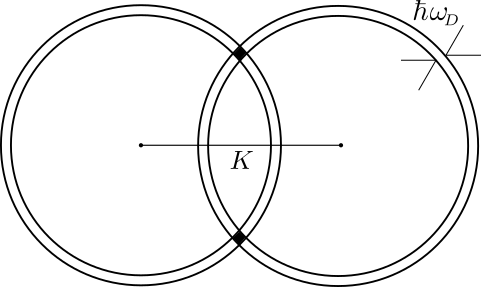
\includegraphics[width=0.6\linewidth]{img/goodcooper.png}
\caption{Construcción geométrica de los posibles electrones candidatos para formar pares de Cooper, siendo $\hbar K$ el momentum del centro de masas.}
\label{fig:goodcooper}
\end{figure}

Otro aspecto de los señalados anteriormente, que podemos abordar ahora, es que los pares estaban formados por electrones no sólo con momenta opuestos, sino también con espines opuestos, esta última característica es ahora muy fácil de tratar, dado que los electrones son fermiones, es decir cumplen el principio de exclusión de Pauli y tienen funciones de onda antisimétricas. Se puede demostrar que la parte orbital (es decir olvidándose de la parte de espín) de la función de onda de los pares de Cooper, depende tan sólo del módulo del momentum. Por lo tanto, frente al intercambio de la posicón de los dos electrones del par se tienen una función simétrica. Luego la parte de espín debe ser antisimétrica, es decir los espines de la pareja son opuestos. Se tiene que un par de Cooper esta formado por dos electrones tal que $k \uparrow, -k \downarrow$.

En este punto surge uno de los peligros típicos de la teoría BCS, que pone de manifiesto la gran cantidad de sutilezas que encierra. Dado que un par de Cooper es una entidad cuyo espin es cero, como los bosones, es fácil caer en la tentación de tratar a los pares de Cooper como bosones. Además hemos indicado que un número creciente de pares de Cooper es energéticamente favorable. Ahora bien, el principio de Pauli sigue vigente: Así, el estado formado, por ejemplo, por $k \uparrow, -k \downarrow$ no puede estar ocupado por más de un par de electrones al mismo tiempo. Además, los operadores con los que se construye el hamiltoniano de la teoría BCS, no siguen las reglas de conmutación de los operadores de bosones. Resulta de todas formas llamativo y conviene resaltarlo que la electrodinámica bosónica reproduce muy bien el comportamiento superconductor, por ejemplo la teoría clásica de la superconductividad de London se puede deducir de un gas cargado de bosones y de allí se puede extraer de una manera natural el efecto Meißner.

Pasaremos a continuación a describir de la manera más sencilla posible la función de onda del estado fundamental superconductor y algunas de las expresiones de la teoría BCS.

La función de onda del estado fundamental de $N$ electrones, según la propone la teoría BCS, es el producto de funciones de onda de pares convenientemente antisimetrizadas, que se puede representar por:

\begin{equation}
    \phi(1,2,...,N) \propto \phi(1,2)\phi(3,4)...\phi(N-1,N)
\end{equation}

Si no escribimos explícitamente la parte de espín y sólo lo hacemos con la parte orbital tendríamos

\begin{equation}
    \phi(1,2,...,N) \propto \sum_{k_1} \sum_{k_2} ... \sum_{k_3} g_{k_1} ... g_{k_{N/2}} e^{i (k_1 r_1 - r_2 k_2 + ... + k_{N/2} r_{N-1} - k_{N/2} r_N)}
\end{equation}

Donde cada término de esta función de onde describe una configuración donde los N electrones se agrupan en $N/2$ pares que son

\begin{equation}
    (k_1, -k_1) ... (k_{N/2}, -k_{N/2})
\end{equation}

La parte de espín es inmediata cada electrón de cada par tiene espines opuestos. Como vemos la funcion de onda es una función complicada que abarca todos los pares relacionados entre ellos. También se puede escribir de una manera más compacta como:

\begin{equation}
    \phi = \prod\limits_k \phi_k
\end{equation}

Antes de continuar merece la pena señalar algún otro aspecto de los pares de Cooper, estos pares están fuertemente relacionados entre sí, de tal manera que se puede decir que del orden de un millón de parestienen sus centros de masa dentro del espacio en el que se extiende un par dado, esto es los pares de electrones que forman un par de Cooer están muy alejados uno del otro, estando fuertemente correlacionados unos pares con otros. Se puede demostrar, que la disminución de la energía en la fase superconductora respecto al estado normal, debida a la interacción entre pares, depende de cómo se elijan esos pares. El conjunto de pares de Cooper no son independientes unos d eotros, están muy correlacionados.

Otro punto que hay que aclarar en lo anterior es que estamos considerando el caso en que no tenemos corriente eléctrica neta, ya que los electrones apareados tienen momentum toal cero. Los estados portadores  decorriente superconductora son aquellos en que los pares tienen momenta que serán $(k + \frac{q}{2} \uparrow, -k + \frac{q}{2} \downarrow)$ y los electrones tendrán una velocidad de arrastre neta que será

\begin{equation}
    v_a = \frac{\hbar q}{2m}
\end{equation}

Otro aspecto importante de la teoria BSC es que predice la existencia de una banda prohibida de energía $\Delta$, la cual se puede medir experimenalmente y que está relacionada con la temperatura crítica por la ecuación BCS. Este parámetro $\Delta$ es el parámetro crucial de la teoría BCS de que acompaña la aparición del esado superconductor.

Hay que resaltar que esta banda reúne unas características muy particulares, por lo pronto se diferencia claramente de las bandas prohibidas que juen un papel importnate en sólidos, especialmente en los semiconductores. En superconductores tenemos una banda prohibida que está situada en la banda de conducción y que tiene una marcada dependencia con la temperatura. Asimismo, mientras que en un semiconductor se necesita excitar por encima de la banda prohibida a los electrones para tener conducción eléctrica, en un superconductor se tiene la supercorriente sin necesidad de tener estados excitados, se tiene conducción eléctrica por debajo del nivel de Fermi, esto es por debajo de la banda prohibida que existe en la banda de conducción.

Este parámetro $\Delta$ aparece en la sencilla e importante relación que se obtiene en la teoría BCS

\begin{equation}
    2 \Delta(0) = 3.52 k_B T_c
\end{equation}

Donde $T_c$ es la temperatura crítica superconductora.

\section{Cuantización del flujo magnético y efecto tunel Giaver}

En la teoría de Ginzburg-Landau \cite{cyrot} de las transiciones de fase se introduce el concepto de parámetro de orden, que es una magnitud que aparece acompañando a la transición. Un ejemplo típico de parámetro de orden es la imanación de saturación, que es la magnitud que aparece cuando se tiene la transición de fase del estado paramagnético al ferromagnético. El modelo macroscópico de la superconductividad está basado en la hipótesis de que existe una función de onda macroscópica $\psi(r,t)$ que describe el comportamiento del ensemble completo de electrones superconductores y que es el parámetro de orden de la transición superconductora, tal que su módulo al cuadrado nos da la densidad de electrones superconductores que aparecen al pasar el metal del estado normal al superconductor. En el estado normal, el parámetro de orden (densidad de electrones superconductores) se desvanece. Por supuesto, esta hipótesis puede ser justificada por la teoría microscópica de la superconductividad (Teoría BCS). Esta teoría se basa en la idea de que en metales superconductores existe una fuerza atractiva entre los electrones cercanos al nivel de Fermi. A temperaturas bajo la temperatura crítica $T_c$, esta fuerza atractiva crea un nuevo estado cuántico diferente del mar de Fermi de un metal normal. Una pequeña porción de los electrones cercanos el nivel de Fermi están ligados a pares de Cooper. En el caso más simple, el movimiento interno de los pares no tiene momentum angular orbital (estado s simétrico) y consecuentemente el principio de Pauli requiere que los dos espines sean opuestos. Contrario a ligar dos átomos a una molécula, el estado orbital del par de Cooper tiene un radio mucho mayor, típicamente entre 10nm y 1$\mu$m, de manera que pares individuales se sobrelapan fuertemente en espacio y por lo tanto, la ligadura resulta cooperativa. En particular, la energía de ligadura de cualquier par depende de cuantos otros pares se hayan condensado y, más aún, el movimiento del centro de masas de los pares está fuertemente correlacionado tal que cada par reside en el mismo estado con el mismo movimiento de centro de masas. Es este estado el que describimos con una función de onda macroscópica y que le da al sistema sus propiedades superfluídicas. Por ejemplo, el movimiento del centro de masas puede ser descrito por la función de onda

\begin{equation}
    \psi(r,t) = \psi_0 e^{i \theta(r,t)} = \psi_0 e^{i k_s \dot r - i \omega t}
\end{equation}

Donde cada par tiene el mismo momentum $\hbar k_s$ o velocidad de par $v_s = \hbar k/m$. Además, se cumple que

\begin{equation}
    n_s = \abs{\psi}^2
\end{equation}
    
Donde $n_s$ es la densidad de electrones superconductores.

Por otro lado, sabemos que la cantidad de movimiento de una partícula de masa $m^*$ y carga $e^*$ en presencia de un campo magnético representado por su potencial vectorial $A$, se escribe como

\begin{equation}
    \mathbf{p} = -i \hbar \nabla \psi(r,t) = \hbar \nabla \phi = m^* \mathbf{v} + \frac{e^*}{c} \mathbf{A}
\end{equation}

Si tenemos una densidad de partículas, todas ellas teniendo el mismo momentum $\mathbf{p}$ podemos escribir $n_s \mathbf{p} = n_s (m^* \mathbf{v} + \frac{e^*}{c} \mathbf{A})$.

Recordando la expresión general de la densidad de corriente eléctrica en función de la densidad de portadores, de la carga y de la velocidad promedio se pueden escribir

\begin{equation}
    \mathbf{J} = n_s e^* \mathbf{v}
\end{equation}

Que en nuestro caso será

\begin{equation}
    \hbar \nabla \phi = \frac{m^*}{n_s e^*} J + \frac{e^*}{c} A
\end{equation}

Con esta expresión estamos preparados para demostrar la cuantización del flujo magnético en superconductores, para ellos basta con recordar algo trivial, como es que el parámetro de orden superconductor sólo puede tener un único valro en cada punto, es decir, la densidad de electrones superconductores debe ser única en cada punto, esta simple consideración se materializa en que podemos escribir

\begin{equation}
    \phi(2\pi) - \phi(0) = n 2 \pi
\end{equation}

Recordando la definición de circulación y de gradiente, y siendo $C$ un camino cerrado, la expresión anterior la podemos escribir como

\begin{equation}
    \oint\limits_C \nabla \phi dl = n 2 \pi
\end{equation}

Si ahora suponemos que este camino $C$ está en el interior de un superconductor, alejado de los bordes y rodeando a un hueco, como se representa en la figura \ref{fig:fluxquant} y suponemos que tenemos aplicado un campo magnético a este superconductor, se tiene

\begin{equation}
    \oint\limits_C (\frac{m^*}{\hbar n_s e^*} J + \frac{e^*}{\hbar e} A) dl = n 2 \pi
\end{equation}

\begin{figure}[H]
\centering 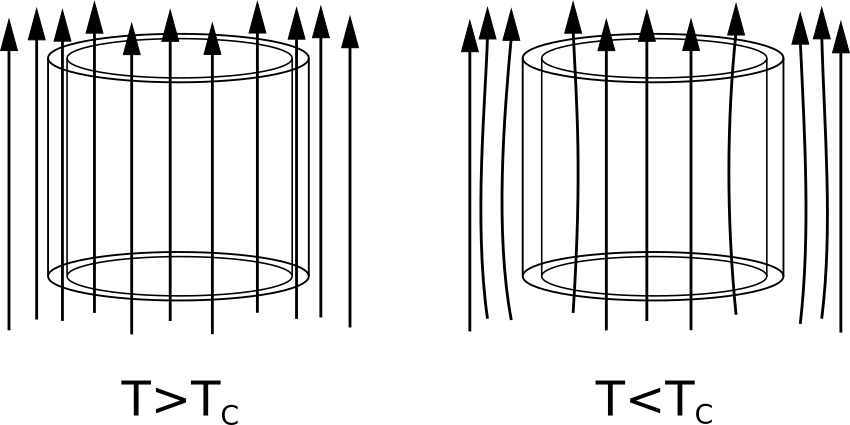
\includegraphics[width=0.8\linewidth]{img/fluxquant.png}
\caption{Cuantización del flujo magnético}
\label{fig:fluxquant}
\end{figure}

Dado que estamos en un camino interior al superconductor y allí no existe corriente (las únicas corrientes que existen en una situación como la que estamos describiendo, están apantallando el campo magnético y están situadas cerca de los bordes tanto de la cavidad como de la superficie del material superconductor), tendremos

\begin{equation}
    \oint A dl = \frac{n h c}{e^*}
\end{equation}

Recordando el teorema de Stokes se tiene

\begin{equation}
    \oint\limits_C A dl = \iint\limits_S B ds = \Phi
\end{equation}

Que en nuestro caso será $\Phi = n \Phi_0$ expresión que nos indica que el flujo magnético que encierra la cavidad es un número entero de un flujo elemental conocido con el nombre de fluxoide y cuyo valor es

\begin{equation}
    \Phi_0 = \frac{h c}{2 e} = 2.07 10^{-7} gauss\ cm^2
\end{equation}

Siendo $e^*$ la carga del portador de corriente, el par de Cooper $e^* = 2e$.

Este efecto fue encontrado experimentalmente de forma simultánea en 1961 por Deaver-Fairbanks \cite{deaver} y por Doll-Näbauer [ref].

El efecto túnel es un efecto típico del carácter cuántico de los electrones, desde el punto de vista de la física clásica es completamente imposible que se produzca el efecto que vamos a discutir.

Los electrones se pueden representar por funciones de onda, de tal manera que existe una cierta probabilidad de que un electrón pueda ir de un metal a otro atravesando una barrera aislante estrecha, que puede ser vacío o un óxido. La función de onda del electrón decae de una manera exponencial fuera de la superficie del metal, la amplitud de la onda no es totalmetne nula fuera del metal, es como si el electrón se desparramase fuera de la superficie. Si situamos un metal junto al otro, separados tan sólo por una barrera, como puede ser, por ejemplo, el óxido de la superficie, existe una probabilidad pequeña, pero no nula de que el electrón atraviese ese túnel y aparezca al otro lado, en el otro metal.

Antes de seguir hay que hacer notar que la energía necesaria para hacer pasar un electrón que está en el nivel de Fermi de un metal al vacío (función de trabajo del metal) es mayor que la energía necesaria para transferir ese electrón a un aislante.

Por razones de simplicidad vamos a hacer toda la discusión siguiente, salvo cuando se diga expresamente lo contrario, para temperatura de 0K. La figura \ref{fig:el1} nos indica la situación entre dos partes del mismo metal separadas por un aislante. Todos los estados por debajo de la energía de Fermi están ocupados, mientras que todos los estados por encima de $E_F$ están vacíos.

\begin{figure}[H]
\centering 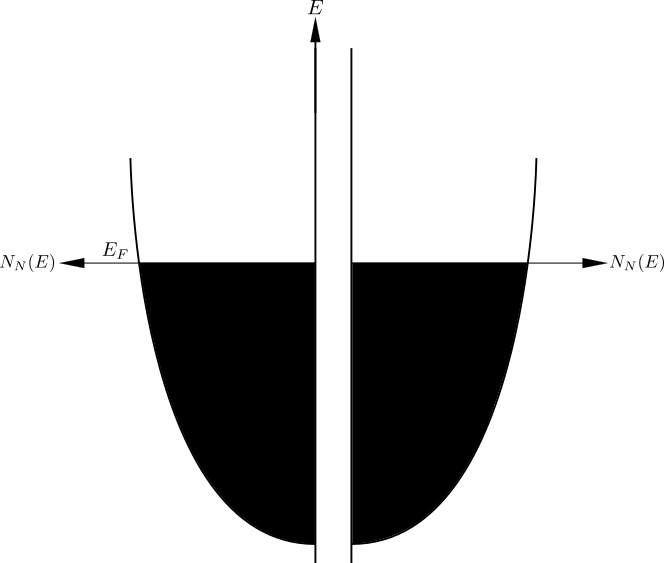
\includegraphics[width=0.8\linewidth]{img/el1.png}
\caption[Diagrama de energía de una junción metal-aislante-metal en la que no puede haber efecto túnel]{Diagrama de energía de una junción metal-aislante-metal en la que no puede haber efecto túnel: En este diagrama ambos lados de la barrera tienen los mismos niveles de energía ocupados. Por lo tanto, no puede haber efecto túnel, porque las transiciones deben ser horizontales y no puede haber dos electrones ocupando elmismo estado.}
\label{fig:el1}
\end{figure}

Para que se pueda tener efecto túnel hacen falta dos condiciones. La primera es que, como es lógico, los electrones solamente pueden ir de un estado ocupado a un estado desocupado y la segund aes que se tiene que conservar la energía, es decir que las transiciones, en la gráfica, tienen que ser horizontales. Por lo tanto en la situación de la figura \ref{fig:el1} no tendremos efecto túnel. No se pueden tener transiciones horizontales al no existir estados vacíos. Todos los estados en el mismo nivel de energía, a ambos lados de la barrera, están ocupados.

Si aplicamos una diferencia de potencial constante a la barrera lo que estamso haciendo es aumentando la energía de los electrones de un lado de la barrera respecto al otro y entonces tenemos la posibilidad de que se tenga corriente por efecto túnel, figura \ref{fig:el2}.

\begin{figure}[H]
\centering 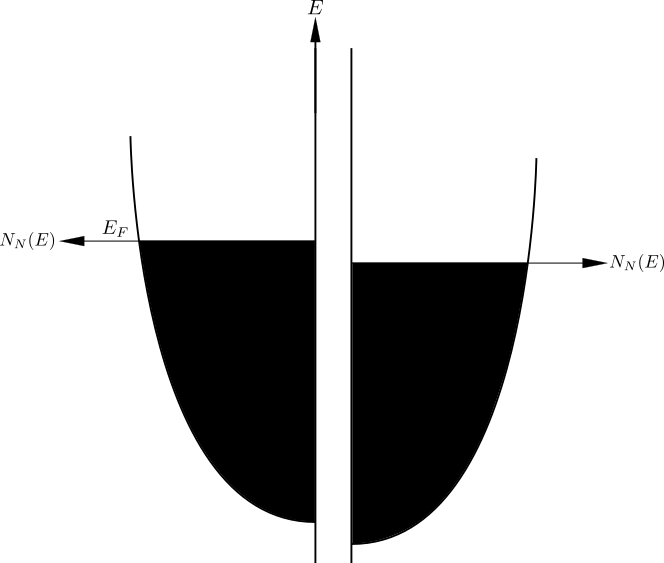
\includegraphics[width=0.8\linewidth]{img/el2.png}
\caption[Diagrama de energía de una junción metal-aislante-metal en la que puede haber efecto túnel]{Diagrama de energía de una junción metal-aislante-metal en la que puede haber efecto túnel: En este diagrama los electrones de uno de los lados de la barrera ocupan niveles de energía más altos que los del otro lado. Por lo tanto, estos electrones pueden pasar al otro lado de la barrera y ocupar los estados que en ese lado se encuentran vacíos.}
\label{fig:el2}
\end{figure}

La intensidad de esta corriente túnel depende de varios parámetros. Por ejemplo, a mayor diferencia de potencial aplicada mayor correitne. Está claro que cuantos más estados tengamos en el nivel de Fermi mayor será la probabilidad de tener corriente túnel, lo cual puede indicar que quizáß con experimentos de efecto túnel podemos obtener información sobre este importante parámetro y en general sobre la superficie de Fermi, pero como es de esperar la corriente túnel también depende de la anchura, altura y forma de la barrera y estos parámetros son muy difíciles de determinar, lo cual hace que en metales normales del efecto túnel se obtenga una información mucho menos rica de lo que se podía esperar. Ocurre todo lo contrario con el efecto túnel cuando uno de los dos metales está en estado superconductor, como pasaremos a ver a continuación.

La existencia de una banda de energía en el estado superconductor \ref{fig:el3} hace que el efecto túnel en una estructura formada por superconductor-aislante-metal en estado normal, tenga características especiales (Giaver, 1960 [ref]). Es claro que necesitamos previamente disponer de electrones normales por encima de la banda prohibida superconductora, esto es hay que romper pares de Cooper, como primera medida, es decir diferencias de potencial aplicadas menores que la banda prohibida no producirán efecto túnel. Esto es, diferencias de potencial aplicadas a la barrera no producen corriente túnel, salvo que venzan un valor umbral, qu es precisamente el ancho de la banda prohibida. De entrada ya tenemos una muy importante propiedad del efecto túnel superconductor, que nos permite medir la banda prohibida superconductora y medir la variación de esta banda con la temperatura.

\begin{figure}[H]
\centering 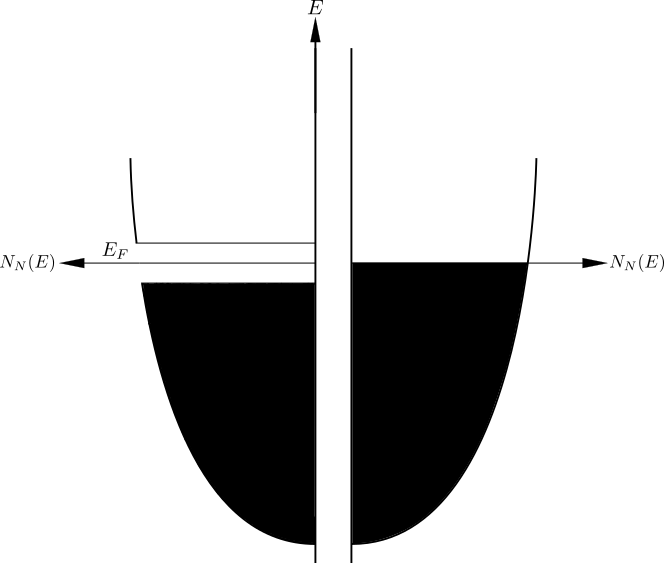
\includegraphics[width=0.8\linewidth]{img/el3.png}
\caption[Diagrama de energía de una junción superconductor-aislante-metal en la que puede haber efecto Giaver]{Diagrama de energía de una junción superconductor-aislante-metal en la que puede haber efecto Giaver: En este diagrama, al producirse excitaciones que lleven electrones por encima de la banda prohibida, rompiendo pares de Cooper, los electrones excitados podrían pasar al otro lado de la barrera por efecto túnel.}
\label{fig:el3}
\end{figure}

\section{Efecto Josephson}

El efecto Josephson fue postulado teóricamente por Josephson (1962) \cite{josephson} y comprobado experimentalmente por P.W. Anderson y Rowell (1963) \cite{rowell} y por Shapiro (1963) \cite{shapiro}, casi simultáneamente. Este es un efecto túnel de pares de Cooper entre superconductores, mientras que el efecto túnel tratado en las líneas anteriores es túnel de electrones normales entre superconductores o entre un metal normal y un superconductor. En concreto la sugerencia de Josephson es que puede existir efecto túnel entre dos superconductores que se encuentren separados por una barrera aislante (en principio más delgada que las tratadas en el efecto túnel Giaver), donde la corriente túnel sea exclusivamente de pares de Cooper sin que se tenga una diferencia de potencial entre ambos lados de la barrera.

Se va a seguir la deducción de Feynman por su sencillez y claridad. Supongamos que tenemos un superconductor separado en dos partes por un aislante lo suficientemente estrecho como para que la función de onda superconductora a un lado de la barrera se sobrelape con la del otro lado. Sean $\psi_1$ y $\psi_2$ las funciones de onda superconductoras a los dos lados de la barrera (1) y (2).

El tunelamiento de pares del lado (2) al lado (1) aumenta la amplitud $\psi_1$ de la función de onda de los pares en el lado (1), es decir, aumenta la cantidad de pares de Cooper en el lado (1). Supongamos que el ritmo de crecimiento de $\psi_1$ es proporcional a $\psi_2$, amplitud de la funcion de onda de los pares en el lado (2). Podemos escribir el ritmo de cambio de $\psi_1$ de la forma $A \psi_2$ donde $A$ es una característica de la barrera y nos da información de la probabilidad de transferencia de pares del lado (2) al lado (1).

Podemos escribir la ecuación de Schrödinger para el lado superconductor (1) teniendo en cuenta esto último, como

\begin{equation}
    \frac{-\hbar}{i} \frac{\partial \psi_1}{\partial t} = E_1 \psi_1 + A \psi_2
\end{equation}

donde $E_1$ es la energía del estado más bajo de energía del superconductor del lado (1).

Análogamente, podemos escribir para el superconductor del lado (2)

\begin{equation}
    \frac{-\hbar}{i} \frac{\partial \psi_2}{\partial t} = E_2 \psi_2 + A \psi_1
\end{equation}

Escribiendo explícitamente la función de onda superconductora, $\psi_i = \sqrt{n_{s_i}} e^{i \varphi_i}$, donde, como ya vimos, $n_{s_i}$ es la densidad de electrones superconductores en el lado (i).

Por lo tanto las ecuaciones anteriores pueden ser escritas como

\begin{align}
    \frac{-\hbar}{i} \frac{1}{2 \sqrt{n_{s_1}}} \frac{\partial n_{s_1}}{\partial t} + \hbar \frac{\partial \varphi_1}{\partial t} \sqrt{n_{s_1}} &= E_1 \sqrt{n_{s_1}} + A \sqrt{n_{s_2}} e^{i (\varphi_2 - \varphi_1)} \\
    \frac{-\hbar}{i} \frac{1}{2 \sqrt{n_{s_2}}} \frac{\partial n_{s_2}}{\partial t} + \hbar \frac{\partial \varphi_2}{\partial t} \sqrt{n_{s_2}} &= E_2 \sqrt{n_{s_2}} + A \sqrt{n_{s_1}} e^{i (\varphi_1 - \varphi_2)}
\end{align}


Si ahora igualamos las partes reales y las partes imaginarias de estas ecuaciones tenemos

\begin{align}
    \frac{\partial \varphi_1}{\partial t} &= \frac{j_0}{2 n_{s_1}} \cos(\delta) + E_1/\hbar \\
    \frac{\partial \varphi_2}{\partial t} &= \frac{j_0}{2 n_{s_2}} \cos(\delta) + E_2/\hbar \\
    \frac{\partial n_{s_1}}{\partial t} &= -j_0 \sin(\delta) \\
    \frac{\partial n_{s_2}}{\partial t} &= j_0 \sin(\delta)
\end{align}

Donde $\delta = \varphi_2 - \varphi_1$ y $j_0 = \frac{2 A}{\hbar} (n_{s_1} n_{s_2})^{\sfrac{1}{2}}$. En lo que sigue, asumiremos que se tiene el mismo superconductor en ambos lados, así que tomaremos $n_{s1} = n_{s2}$. Entonces:

\begin{align}
    \frac{\partial \delta}{\partial t} &= \frac{\partial \varphi_2}{\partial t} - \frac{\partial \varphi_1}{\partial t} = (E_2 - E_1)/\hbar \\
    j &= \frac{\partial n_{s_2}}{\partial t} = - \frac{\partial n_{s_1}}{\partial t} = j_0 \sin(\delta)
\end{align}

De aquí salen directamente las relaciones de Josephson para corriente y voltaje:

\begin{align}
    V_J &= \frac{\hbar}{2e} \frac{\partial \delta}{d t} \\
    I_J &= I_0 \sin(\delta)
\end{align}

Donde el voltaje $V_J$ es la diferencia de potencial entre los dos extremos de la junción de Josephson e $I_J$ es la supercorriente que fluye a través de ésta.

Existe una clara diferencia entre este efecto túnel y el considerado al principio. En este caso de efecto Josephson tenemos túnel de pares de Cooper, mientras que en el caso anterior el túnel era de electrones individuales. En el efecto Josephson son bastante estrechas del orden o menores que la longitud coherente (tamaño de los pares de Cooper), en realidad el aislante actúa como un mal superconductor, las funciones de onda de ambos lados se pueden solapar, existiendo una difrencia de fase a ambos lados de la barrera y como resultado de todo esto se establece una corriente continua a través de la barrera. En ralidad, se puede demostrar que el mínimo de enrgía se alcanza cuando las fases se igualan y por lo tanto no se tiene correitne a través de la barrera, pero basta con aplicar una correinte de una fuente externa, siempre menor que $I_0$, para que las fases dejen de ser iguales y si esta desigualdad no varía con el tiempo, se tiene a través de la barrera una correitne constante sin que se tenga caída de potencial. no hace falta colocar un óxido, un aislante, para que actúe de barrera se puede utilizar un estrechamiento en el supercondcutor, producido mediante una técnica conocida como fotolitografía, o cualquier otra técnica que nos produzca que una parte del supercondutor esté unida a otra mediante un estrangulamiento lo suficientemente estrecho como para ser una unión débil. También se peuden obtener este tipo de uniones débiles con contactos entre superconductores de tipo puntual, o bien separando dos supercondcutores por una capa delgada de un metal en estado normal. Como acabamos de mencionar el tamaño de los pares de Cooper es una indicación del orden de magnitud de esta unión débil.

Los órdenes de magnitud de los parámetros que intervienen en el efecto Josephson son, para una unión de $1mm^2$ de área $R = 1 \Omega$, $I_0 = 1 mA$ y $\Delta = 1meV$. Normalmente las densidades de corriente a través de las uniones son dle orden de un millón de veces menores que las densidades de corriente crítica superconductoa en un superconductor. Es decir, en general, en un superconductor se tiene que pasar de la densidad de correinte crítica para hacer desaparecer la superconductividad, pero si el superconductor tiene en algún punto una unión débil densidades de corriente un millón de veces menores hacen que se tenga caída de potencial en el paso de correitne por la unión.

Si hacemos pasar una corriente mayor que $I_0$ aparece una diferencia de potencial y teniendo en cuenta que al mismo tiempo que este efecto túnel (Josephson) de pares podemos tener el efecto túnel normal (Giaver) de electrones, el resultado se puede ver en la figura \ref{fig:ivjj} donde se representa la curva característica I,V. Como sea la conexción en la realidad entre estos dos túneles depende de las características de l aunión y del circuito exterior.

\begin{figure}[H]
\centering 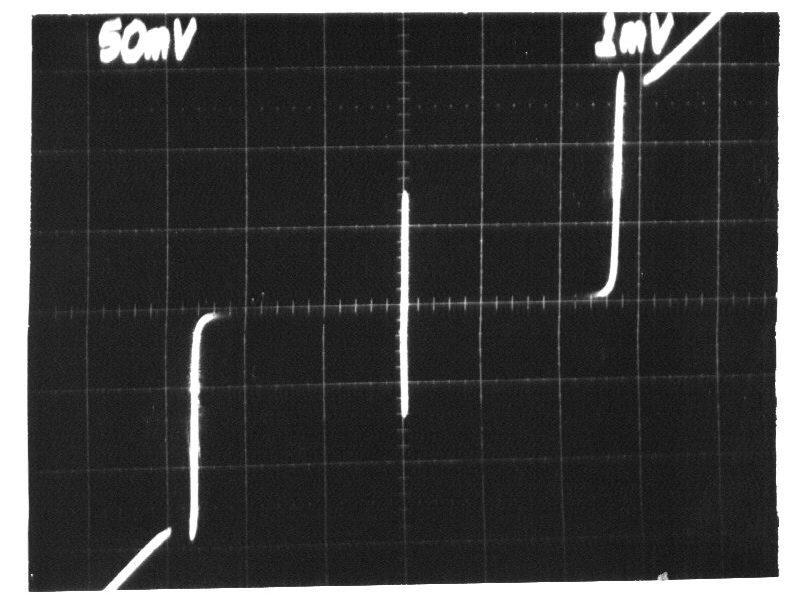
\includegraphics[width=0.8\linewidth]{img/IVJJ.JPG}
\caption[Curva característica I-V de una unión Josephson]{Curva característica I-V de una unión Josephson: El eje vertical tiene una escala de $50\mu A$ y el ejevertical 1mV. La barra en $V=0$ corresponde a la supercorriente producida por efecto Josephson. Para $V > 3mV$ se entra en el régimen ohmico de la unión de Josephson, el cuál se produce por el tamaño finito de la banda prohibida}
\label{fig:ivjj}
\end{figure}

Finalmente hay que considerar lo que ocurre si aplicamos a la unión Josephson una diferencia de potencial externa constante, V, o lo que es lo mismo, tenemos una intensidad pasando por la barrera superor a $I_0$. El cálculo es análogo al anterior, muy sencillo y nos conduce a que la intensidad a través de la barrera tiene la expresión

\begin{equation}
    I = I_0 \sin( (\varphi_2 - \varphi_1) + \omega t) = I_o \sin(\delta + \omega t)
\end{equation}

Donde $\omega = \frac{2 eV}{\hbar}$. En realidad el punto de partida de esta deducción es la dependencia con el tiempo de la fase, una diferencia de potencial aplicada a l aunión lo que hace es variar en el tiempo la fase y el ritmo de variación d ela fase viene dado por la ecuación $\frac{d \delta}{d t} = \frac{E_2 - E_1}{\hbar} = \frac{qV}{\hbar} = \frac{2 eV}{\hbar}$.

Es decir, una diferencia de potencial constante aplicada a una barrera Josephson produce una corriente alterna de pares (una supercorreinte), por ejemplo una diferencia de potencial del orden de $1 \mu V$ da lugar a una corriente que oscila con una frecuencia de 484MHz. Además de esta corriente de pares tenemos la correitne debida al efecto túnel normla de los electrones individuales. Ahora podemos volver a la figura \ref{fig:ivjj} donde tendremos que hasta que se alcanza el valor $I_0$ tenemos paso de correinte por la unión sin caida de potencial. una vez que $I > I_0$, entonces aparece un voltaje y nos situamos en un punto de la gráfica del efecto túnel de electrones normales (Giaver), tenemos una diferencia de potencial aplicada, luego existe túnel normal y además, esto no está represntado en la fëáfica, tenemos una supercorriente (corriente de pares de Cooper) que está oscilando.

\section{Componentes de la corriente en las junciones de Josephson}

La corriente en las junciones Josephson tiene tres componentes:

\begin{enumerate}
    \item $I_d$, la corriente de desplazamiento: Como la corriente en un capacitor. La junción de Josephson forma un capacitor de placas parelelas superconductoras con un material aislante o un metal normal entre ellas, entonces podemos hablar de una corriente de desplazamiento $I_d$. La capacitancia $C$ de este dispositivo está definida de la misma manera que en el estado normal: $C = \epsilon_r \frac{A}{4 \pi d}$, donde $\epsilon_r$ es la constante dieléctrica relativa de la capa que separa a los dos superconductores, $d$ la separación de los superconductores y $A$ el área de los mismos.
    \item $I_n$, la correinte ordinaria: Por los electrones individuales. Cuando la temperatura $T \neq 0$, siempre habrá movimiento térmico de cargas cuya energía es del orden de $k_b T$, donde $k_B$ es la constante de Boltzmann. Cuando $T$ es menor, pero cercano a la termperatura crítica $T_c$, la energía de acoplamiento de los pares de Cooper $E_g = 2 \Delta$ es mucho menor a $k_B T$, lo cual resulta en la disminución de los pares de Cooper y el aumento de la concentración de eletrones normales. Si el voltaje a través de la junción es mayor al asociado a la energía de la brecha $V_g = \abs{\Delta_1 + \Delta_2}/e$, los pares de Cooper de un lado de la unión se rompen y uno de los electrones de cada uno de los pares disueltos pasa al otro lado, es decir, se produce un tunelamiento de electrones normales. Si la concentración de electrones individuales aumenta, el comportamiento de la unión tenderá a uno de tipo óhmico, es decir, la junción tenderá a comportarse como una resistencia.
    \item $I_s$, la supercorriente: Por los pares de Cooper. Se puede expresar en términos de una corriente crítica $I_0$ y la diferencia de fase entre las funciones de onda macroscópicas de las dos placas superconductoras, de manera que $I_s = I_0 \sin(\delta)$. La corriente crítica es un parámetro experimental importante del dispositivo que puede alterarse tanto por la temperatura como por un campo magnético aplicado.
\end{enumerate}

\section{Qubits superconductores}
Los qubits superconductores se basan en circuitos osciladores no lineales, hechos a partir de junciones Josephson \cite{wendin}.

El Hamiltoniano de un oscilador armónico LC está dado por 

\begin{equation}
\hat{H} = E_C \hat{n}^2 + E_L \frac{\hat{\phi}^2}{2},
\end{equation}

donde $\hat{n}$ es la cantidad de pares de Cooper inducidos en el capacitor (En otras parabras, la carga inducida en el capacitor, medida en unidades de $2e$), y $\hat{\phi}$ es la diferencia de fase sobre el inductor. La carga $\hat{n}$ y la fase $\hat{\phi}$ no conmutan, $\comm{\hat{\phi}}{\hat{n}}=i$, lo que significa que sus valores esperados no se pueden medir simultaneamente. $E_C=\frac{(2e)^2}{2C}$, $E_L=\frac{\hbar^2}{(2e)^2L}$ y la distancia entre niveles de energía del oscilador armónico $\hbar \omega = \frac{\hbar}{\sqrt{LC}}=\sqrt{2E_LE_C}$.

Para poder servir como qubit, el oscilador debe ser anarmónico, de manera que se pueda operar sobre un par específico de niveles de energía. Al agregar una junción Josephson, el Hamiltoniano del circuito LCJ se convierte en:

\[
\hat{H} = E_C (\hat{n}-n_g)^2 - E_{J0} \cos( \hat{\phi} ) + E_L \frac{(\hat{\phi}-\phi_e)^2}{2},
\]

donde $n_g$ es la carga inducida por voltaje en el capacitor C (isla qubit) y $\phi_e$ es la fase inducida por flujo sobre la junción Josephson. La energía de Josephson $E_{J0}$ está dada por $E_{J0}=\frac{\hbar}{2e}I_0$ en términos de la corriente crítica $I_0$ de la unión. Usualmente, la junción Josephson es del tipo Superconductor-Aislante-Superconductor con corriente crítica fija.

Con el fin de introducir la inductancia no lineal de Josephson, empezamos por 

\[
I_J = I_0 \sin(\phi)
\]

Combinado con la ley de Lenz:

\[
V = \frac{d\Phi}{dt} = \frac{\Phi_0}{2\pi} \frac{d\phi}{dt}, \hspace{20pt} \Phi_0=\frac{h}{2e}
\]

Se encuentra que:

\[
V = \frac{\Phi_0}{2\pi} \frac{1}{I_0\cos(\phi)} \frac{dI_J}{dt}
\]

Definiendo $L_J = V (\frac{dI_J}{dt})^{-1}$, se obtiene finalmente la inductancia de Josephson $L_{J0}$:

\[
L_J = \frac{\Phi_0}{2\pi} \frac{1}{I_0 \cos(\phi)} = L_{J0} \frac{1}{\cos(\phi)}
\]

Esto define la inductancia de Josephson de la junción Josephson aislada y nos permite expresar la energía de Josephson como $E_{J0} = \frac{\hbar^2}{(2e)^2L_{J0}}$

\begin{align}
[E_C (-i\hbar \frac{\partial}{\partial\phi}-n_g)^2 + U(\phi)] \psi = E \psi \\
U(\phi) = -E_{J0} \cos(\phi) + E_L \frac{(\phi-\phi_e)^2}{2}
\end{align}

De aquí podemos distinguir los siguientes dos casos principales:

\begin{enumerate}
    \item $E_L = 0 \quad (L \sim \infty)$: En este caso $U(\phi)$ se convierte en una potencial de tipo coseno puro. La función de onda tiene la forma $\psi = \psi(\phi, n_g) e^{i n_g \phi}$, donde $\psi(\phi, n_g)$ es una función de Mathieu. Los niveles de energía forman bandas $E(n_g)$ en la dirección ``momentum''. La dispersión de estas bandas depende del cociente $E_{J0}/E_C$. Es de especial interés el caso en el que la capacitancia $C$ es grande, pues esto resulta en bandas planas, lo cual protege al circuito de ruidos causados por fluctuaciones en la carga.
    \item $E_L \approx E_{J0}$: En este caso $U(\phi)$ deja de ser periodico y describe una parábola modulada por una función sinusoidal. La forma de este potencial cerca del fondo de la parábola y la estructura de los niveles de energía del qubit dependen altamente del cociente $E_L/E_{J0}$ y del flujo externo $\phi_e$. Esto permite crear distintos tipos de qubits con una gran variedad de parámetros distintos.
\end{enumerate}

\section{Arquetipos de qubits superconductores}

Existen tres arquetipos principales de qubit superconductores. Ellos son los siguientes:

\subsection{Qubit de carga}

Si $E_L$ tiende a cero, la carga almacenada en la isla superconductora entre el capacitor y  la unión Josephson se puede usar como qubit. El potencial de este tipo de qubit es de forma de coseno. Los transmones son un tipo particular de qubit de carga.

\subsection{Qubit de flujo}

Si $E_L$ es comparable con $E_{J0}$, el flujo a través del lazo formado por el inductor y la unión Josephson se puede usar como qubit. El potencial de este tipo de qubit es de forma cuártica.

\subsection{Qubit de fase}

Si se polariza la unión Josephson con una fuente de corriente, la fase en ambos extermos de la unión Josephson se puede usar como qubit. El potencial de este tipo de qubit es de forma cúbica.

\section{Transmones}

Los transmones son un tipo de qubit de carga derivado capacitivamente para hacerlo insensible a las fluctuasiones de carga. La manera de interactuar con los transmones es acoplándolos a un resonador. Tratando el transmón como un sistema de dos niveles y el resonador como un oscilador monomodo, podemos modelar este sistema con el Hamiltoniano de Jaynes-Cummings, el cuál describe un átomo o un átomo artificial que interactúa con un oscilador armónico cuántico:

\begin{equation}
    \hat{H} = \hat{H}_q + \hat{H}_{qr} + \hat{H}_r = -\frac{1}{2} \hbar \omega_q \sigma_z + \hbar g \sigma_x (a+a^\dag) + \hbar \omega_r (a^\dag a + \frac{1}{2})
\end{equation}

donde $\omega_q$ es la frecuencia de resonancia del qubit, $g$ es la constante de acoplamiento qubit-oscilador y $\omega_r$ es la frecuencia de resonancia del resonador. El operador $a$ es el operdor de aniquilación bosónico del oscilador y su efecto al ser aplicado al estado del sistema es aniquilar fotones del resonador. Similarmente, $a^\dagger$ es el operador de creación bosónico del oscilador y su efecto al ser aplicado al estado del sistema es crear fotones en el resonador.

\begin{align}
    a \ket{n} &= \sqrt{n} \ket{n-1} \\
    a^\dagger \ket{n} &= \sqrt{n+1} \ket{n+1}
\end{align}

Aquí $n$ es la cantidad de fotones en el resonador. De estas ecuaciones podemos deducir el operador de número, el cuál es:

\begin{equation}
    a^\dagger a \ket{n} = a^\dagger \sqrt{n} \ket{n-1} = \sqrt{(n-1)+1} \sqrt{n-1} \ket{(n-1)+1} = n \ket{n}
\end{equation}

En cuando a los operadores del qubit, tenemos el operador de aniquilación fermiónico $\sigma_-$, el cuál disminuye el nivel de energía del qubit, y el operador de creación fermiónico $\sigma_+ = \sigma_-^\dagger$, el cuál aumenta el nivel de energía del qubit.

\begin{align}
    \sigma_- &= \ketbra{0}{1} \\
    \sigma_+ &- \ketbra{1}{0}
\end{align}

También tenemos el operador $\sigma_z$, que es el análogo del operador de número para el qubit y el operador $\sigma_x$ que hace un \textit{bitflip}.

\begin{align}
    \sigma_z &= \ketbra{0} - \ketbra{1} = \sigma_-\sigma_+ - \sigma_+\sigma_- \\
    \sigma_x &= \ketbra{0}{1} + \ketbra{1}{0} = \sigma_- + \sigma_+
\end{align}

El término de interacción del Hamiltoniano de Jaynes-Cummings lo podemos descomponer en el término de Jaynes-Cummings y el término anti-Jaynes-Cummings.

\begin{equation}
    \hat{H}_{qr} = \hat{H}_{qr}^{JC} + \hat{H}_{qr}^{AJC} = g(\sigma_+ a + \sigma_- a^\dag) + g(\sigma_+ a^\dag + \sigma_- a)
\end{equation}

El término $H_{qr}^{AJC}$ describe oscilaciones de alta frecuencia. En los sistemas típicos, estas oscilaciones están en el orden de los teraherzios (THz) y tienen amplitudes muy pequñas. Debido al orden de las frecuencias de estas oscilaciones, no las podemos medir con la tecnología utilizada para la computación cuántica. Las mediciones en el régimen de los teraherzios son un tema de investigación activo en el que todavía nos estamos adentrando [ref]. Por esto y la amplitud despreciable de estas oscilaciones, es común hacer la aproximación de onda rotativa, con la cual se aplica una transformación al Hamiltoniano de manera que desaparesca el término $H_{qr}^{AJC}$. Trabajaremos con el Hamiltoniano de Jaynes-Cummings bajo esta aproximación. Además, también usaremos unidades naturales, es decir, que tendremos que $\hbar = 1$ y $c = 1$, donde $\hbar$ es la consante reducida de Planck y $c$ es la velocidad de la luz. En estas unidades la energía se mide en Hz.

\begin{equation}
    \hat{H}_{RWA} = \hat{H}_r + \hat{H}_q + \hat{H}_{qr} = \omega_r a^\dag a - \frac{1}{2} \omega_q \sigma_z + g(a \sigma_+ + a^\dag \sigma_-)
\end{equation}

En este Hamiltoniano tenemos el término $\hat{H}_r = \omega_r a^\dagger a$, correspondiente a la energía del resonador. Este término da la cantidad de fotones de frecuencia $\omega_r$ en el resonador y por lo tanto, la energía de este subsistema (recordemos que elegimos $\hbar = 1$). En el primer Hamiltoniano que presentamos también había un término $+ \frac{1}{2} \omega_r$, este término se puede descartar, pues sólo representa un término constante de energía y como es una constante por la identidad, sólo actúa como una fase global en la evolución del sistema, así que no afecta las probabilidades. El término $\hat{H}_q = - \frac{1}{2} \omega_q \sigma_z$ representa la energía del qubit. $\omega_q$ es la diferencia de energía entre los dos niveles del qubit y el nivel cero de energía se ha tomado tal que el espectro del qubit esté centrado alrededor del cero. Así, el qubit tiene energía $-\frac{1}{2} \omega_q$ cuando está en el estado $\ket{0}$ y energía $\frac{1}{2} \omega_r$ cuando está en el estado $\ket{1}$. Finalmente, el término de interacción $H_{qr} = g (a \sigma_+ + a^\dagger \sigma_-)$ indica que las emisiones en el resonador corresponden a absorsiones del qubit y viceversa. La manera en la que interactúan el resonador y el qubit es intercambiando energía.

\section{Hamiltonianos multiqubit de transmones}

Cuando tenemos más de un qubit acoplado al mismo resonador, estos interactúan virtualmente a través de emisiones y absorsiones con el resonador. Omitiendo el término del oscilador, esto se refleja en el Hamiltoniano, de forma general, de la siguiente manera:

\begin{equation}
\hat{H} = \hat{H}_q + \hat{H}_{qr} + \hat{H}_{qq} = -\frac{1}{2} \sum\limits_i \epsilon_i \sigma_{zi} + \sum\limits_i g_i \sigma_{xi} (a+a^\dag) + \frac{1}{2} \sum\limits_{i,j;\nu} \lambda_{\nu,ij} \sigma_{\nu i} \sigma_{\nu j}
\end{equation}

Por simplicidad, se considera que el término $\hat{H}_{qr}$ se refiere sólo a la lectura y las operaciones de bus, dejando la interacción indirecta qubit-qubit via el resonador ser incluidas en $\hat{H}_{qq}$ via la constante de acoplamiento $\lambda_{\nu,ij}$. Existen distintos tipos de acoplamiento qubit-qubit, entre ellos se encuentran los siguientes:

\begin{enumerate}
    \item Acoplamiento capacitivo

        Este acoplamiento se logra conectando transmones con un capacitor y tiene el siguiente término de interacción:

        \begin{align*}
            \hat{H}_{qq} &= \lambda_{1 2} \sigma_{x1} \sigma_{x2} \\
            \lambda_{1 2} &= \frac{1}{2} \sqrt{E_{1 0, 1} E_{1 0, 2}} \frac{\sqrt{E_{E_{C1}} E_{E_{C2}}}}{E_{Cc}} \\
                          &= \frac{1}{2} \sqrt{E_{1 0, 1} E_{1 0, 2}} \frac{Cc}{\sqrt{C_1 C_2}} \approx \frac{1}{2} E_{1 0} \frac{C_c}{C} \\
            \hat{H}_{qq} &= \lambda_{1 2} (\sigma_{+1} \sigma_{-2}  + \sigma_{-1} \sigma_{+2})
        \end{align*}

    \item Acoplamiento por el resonador

        Este acoplamiento se logra conectando transmones a un mismo resonador a modo de bus y tiene el siguiente término de interacción:

        \begin{align*}
            \hat{H}_{qq} &= \lambda_{1 2} \sigma_{x1} \sigma_{x2} \\
            \lambda{1 2} &= \frac{1}{2} g_1 g_2 (\frac{1}{\Delta_1} + \frac{1}{\Delta_2} \equiv g_1 g_2 \frac{1}{\Delta}) \\
            \Delta_i &= \epsilon_i - \hbar \omega
        \end{align*}

    \item Acoplamiento de junción Josephson

        Este acoplamiento se logra conectando transmones con una junción Josephson y tiene el siguiente término de interacción:

        \begin{align*}
            \hat{H}_{qq} &= \lambda_{1 2} \sigma_{y1} \sigma_{y2} \\
            \lambda_{1 2} &\approx \frac{1}{2} E_{1 0} \frac{L_c}{L_J} \frac{\cos(\delta_c)}{2L_c \cos(\delta_c) + L_{J c}}
        \end{align*}
\end{enumerate}

\section{Compuertas cuánticas en transmones}

Las compuertas cuánticas se construyen agregando términos al Hamiltoniano del sistema de manera que el operador de evolución de un tiempo $t_0$ a un tiempo $t_1$ sea igual al operador de la compuerta deseada. La evolución temporal de un sistema cuántico puede ser descrita por la ecuación de Schrödinger para el vector de estado $\ket{\psi(t)}$:

\[
i \hbar \frac{\partial}{\partial t} \ket{\psi(t)} = \hat{H}(t) \ket{\phi(t)}
\]

en términos del operador evolución $\hat{U}(t,t_0)$

\[
\ket{\psi(t)} = \hat{U}(t,t_0) \ket{\psi(t_0)}
\]

El Hamiltoniano del sistema lo podemos descomponer en los siguientes términos:

\[
\hat{H} = \hat{H}_{syst} + \hat{H}_{ctrl}(t)
\]

Los cuales describen al sistema intrínseco, $\hat{H}_{syst}$ y las operaciones de control aplicadas, $\hat{H}_{ctrl}$. Las compuertas son el resultado de aplicar pulsos de control específicos a partes selectas de un circuito físico. Esto afecta varios términos del Hamiltoniano, haciéndolos dependientes del tiempo. En general, los términos de control se pueden escribir como:

\[
\hat{H}_{ctrl} = \sum\limits_{i; \nu} f_{\nu i}(t) \sigma_{\nu i} + \frac{1}{2} \sum\limits_{i,j;\nu} h_{\nu, ij}(t) \sigma_{\nu i} \sigma_{\nu j} + k(t) a^\dag a
\]

Pulsos de microondas

$$\hat{H}_d = \sum\limits_k (a+a^\dagger) (\xi_k e^{-i\omega_d^{(k)}t} + \xi_k^*e^{i\omega_d^{(k)}t})$$

RWA: $$\hat{H}_d=\sum\limits_k a\xi_k^*e^{i\omega_d^{(k)}t}+ a^\dagger\xi_ke^{-i\omega_d^{(k)}t}$$

En el apéndice \ref{ch:hamiltonians} se realizan con detalle los cálculos asociados a la deducción del Hamiltoniano efectivo que dará lugar a las compuertas que construiremos. Un bus de transmones controlado con pulsos de microondas y con frecuencias de resonancia modulables tendrá el siguiente Hamiltoniano efectivo con el que podemos realizar rotaciones en X-Y y la compuerta de entrelazamiento $\sqrt{iSWAP}$.

\begin{multline}
\hat{H}_{eff} = \tilde{\tilde{\Delta}}_r a^\dagger a - \frac{1}{2} \sum\limits_i \Delta_{qi} \sigma_{zi} + \sum\limits_i g_i (a \sigma_{+i} + a^\dagger \sigma_{-i}) + \sum\limits_i (\Omega \sigma_{+i} + \Omega^* \sigma_{-i}) + \\
\sum\limits_{ij} \frac{g_i g_j}{2 \Delta_j} \left(\sigma_{+i} \sigma_{-j} + \sigma_{+j} \sigma_{-i}\right)
\end{multline}

En este Hamiltoniano $\tilde{\Delta}_r$ es la diferencia entre las frecuencias del resonador, con un pequeño desplazamiento $\chi$ dependiente del estado de cada qubit, y la del pulso de control aplicado. De igual manera, $\Delta_{qi}$ es la diferencia entre la frecuencia de resonancia de cada qubit y la frecuencia del pulso aplicado. $\Delta_i$ es la diferencia entre la frecuencia de cada qubit y la del resonador. El término $\sum\limits_{ij} \frac{g_i g_j}{2 \Delta_j} \left(\sigma_{+i} \sigma_{-j} + \sigma_{+j} \sigma_{-i}\right)$ representa el acoplamiento por el resonador entre los qubits. El término $\sum\limits_i (\Omega \sigma_{+i} + \Omega^* \sigma_{-i})$ representa el efecto del pulso de control sobre los qubits.

\subsection{Rotaciones X-Y}

Tomando $\Omega(t) = \Omega^x(t) \cos(\omega_d t) + \Omega^y \sin(\omega_d t)$, donde $\omega_d$ es igual a la frecuencia de resonancia de uno de los qubits logramos rotaciones sobre los ejes X e Y. Las amplitudes de estas rotaciones vienen dadas por $\int_0^{t_0} \Omega^x(t) dt$ y $\int_0^{t_0} \Omega^y(t) dt$, respectivamente, donde $t_0$ es la duración del pulso.

Tomemos un pulso modulado de la siguiente manera $\Omega(t) = \Omega^x(t) \cos(\omega_d t) = \frac{\Omega^x(t)}{2} (e^{i \omega_d t} + e^{-i \omega_d t})$, donde $\omega_d$ coincide con la frecuencia de resonancia de alguno de los qubits. El término correspondiente en el Hamiltoniano será $\frac{1}{2} (\Omega^x(t) \sigma_{+i} + \Omega^x(t) \sigma_{-i}) = \frac{\Omega^x(t)}{2} \sigma_{xi}$. Generando así, rotacione en X para el qubit i. Si variamos la fase del pulso, tal que $\Omega(t) = \Omega^k(t) \cos(\omega_d t + \phi_k)$, entonces podremos generar rotaciones alrededor de cualquier eje del plano X-Y dentro de la esfera de Bloch. Por ejemplo, sea $\phi_y = \pi/2$, entonces tendremos $\Omega(t) = \Omega^y(t) \sin(\omega_d) = \frac{\Omega^y(t)}{2} \frac{-i e^{i \omega_d t} + i e^{i \omega_d t}}{2i}$. Así, el termino en el Hamiltoniano será $\frac{\Omega^y(t)}{2} (-i \sigma_{-i} + i \sigma_{+i}) = \frac{\Omega^y(t)}{2} \sigma_{yi}$. Por lo tanto, aplicando pulsos modulados en fase y cuadratura podemos generar rotaciones en X-Y tales que

\begin{equation}
    \hat{H}_{XY} = \frac{1}{2} (\Omega^x(t) \sigma_x + \Omega^y(t) \sigma_y)
\end{equation}

Lo cual nos ta la siguiente contribución a la evolución del sistema:

\begin{equation}
    \hat{H}_{XY} = \frac{1}{2} (\Omega^x(t) \sigma_x + \Omega^y(t) \sigma_y)
\end{equation}

\subsection{Compuerta de entrelazamiento}

Ahora estudiemos lo que sucede si modulamos la frecuencia de resonancia de dos qubits en el mismo valor, así que $\Delta_1 = \Delta_2 = \Delta$ y sea $J = \frac{g_1 g_2}{\Delta}$. Vamos a enfocarnos en el término de acoplamiento por el resonador entre estos dos qubits.

\begin{equation}
    \hat{H}_{q_1 q_2} = (\frac{g_1 g_2}{2 \Delta_1} + \frac{g_1 g_2}{2 \Delta_2}) (\sigma_{-_1} \sigma_{+_2} + \sigma_{+_1} \sigma_{-_2}) = J (\sigma_{-_1} \sigma_{+_2} + \sigma_{+_1} \sigma_{-_2})
\end{equation}

Este elemento contribuirá a la evolución del sistema de la siguiente manera:

\begin{equation}
    U(t_1, t_0) = e^{-i J (\sigma_{-_1} \sigma_{+_2} + \sigma_{+_1} \sigma_{-_2}) (t_1 - t_0)} = 
    \begin{pmatrix}
        1 & 0 & 0 & 0 \\
        0 & \cos(J (t_1 - t_0))  & -i \sin(J (t_1 - t_0)) & 0 \\
        0 & -i \sin(J (t_1 - t_0)) & \cos(J (t_1 - t_0)) & 0 \\
        0 & 0 & 0 & 1 \\
    \end{pmatrix}
\end{equation}

Por lo que si tomamos $t_1$ y $t_0$ tales que $t_1 - t_0 = \frac{\pi}{4J}$ podemos generar la compuerta $\sqrt{iSWAP}$

\begin{equation}
    U(t_0 + \frac{\pi}{4J}, t_0) = 
    \begin{pmatrix}
        1 & 0 & 0 & 0 \\
        0 & \frac{1}{\sqrt{2}}  & -i \frac{1}{\sqrt{2}} & 0 \\
        0 & -i \frac{1}{\sqrt{2}} & \frac{1}{\sqrt{2}} & 0 \\
        0 & 0 & 0 & 1 \\
    \end{pmatrix} = \sqrt{iSWAP}
\end{equation}

Intuitivamente sigue que si dejamos que esta interacción ocurra por el doble de tiempo, es decir $t_1 - t_0 = \frac{\pi}{2J}$ generaremos la compuerta iSWAP.

\begin{equation}
    U(t_0 + \frac{\pi}{2J}, t_0) = 
    \begin{pmatrix}
        1 & 0 & 0 & 0 \\
        0 & 0 & -i & 0 \\
        0 & -i & 0 & 0 \\
        0 & 0 & 0 & 1 \\
    \end{pmatrix} = iSWAP
\end{equation}

\subsection{Compuertas compuestas}

Con los transmones se pueden realizar rotaciones X-Y y la compuerta iSWAP. Sin embargo, los algoritmos no se escriben en función de sólo estas compuertas, también se necesitan H, CNOT, entre otras. Entonces, debemos construir estas otras compuertas en función de Rx, Ry e iSWAP. Esto es posible, ya que con secuencias de rotaciones en X e Y se puede realizar cualquier compuerta de un sólo qubit, ya que estas consisten de rotaciones en la esfera de Bloch y con rotaciones sobre dos ejes ortogonales se pueden lograr rotaciones sobre cualquier eje en la esfera. Luego, con un conjunto universal de compuertas de un sólo qubit y una compuerta de entrelazamiento, se tiene un conjunto universal de compuertas cuánticas.


\chapter{El simulador}

El simulador se construyó utilizando la librería Qutip 4.2 de Python 3.6. Esta es una librería que incluye varias herramientas para realizar simulaciones de sistemas mecánico cuánticos, entre ellas, un solucionador de ecuaciones maestras. El funcionamiento básico del simulador desarrollado es el siguiente:

\begin{enumerate}
    \item Leer estado inicial
    \item Construir Hamiltoniano del sistema
    \item Introducir Hamiltoniano y estado inicial en el solucionador de ecuaciones maestras.
    \item Retornar solución
\end{enumerate}

De esta manera se simulan las compuertas naturales de los transmones. Luego, a partir de estas se construyen todas las demás compuertas que se necesitaran para construir un conjunto de compuertas cuánticas con el cual poder ejecutar los algoritmos de Grover, Shor y PageRank.

Se simularon dos sistemas distintos, uno de cuatro qubits y otro de ocho qubits. El diseño original era el de cuatro qubits, con él se realizaron las simulaciones del algoritmo de Grover y del PageRank. Sin embargo, el algoritmo de Shor requiere de al menos ocho qubits para factorizar el número compuesto impar más pequeño: el número 15. Posteriormente también se realizo una generalización del simulador para poder trabajar con sistemas de n qubits.

El tipo de acoplamiento entre los qubits elegido es el acoplamiento de tipo bus. De esta manera trabajamos con un único resonador, el cual se puede tracear. Esto reduce significativamente la dimensión del sistema a simular y nos permite tener más qubits. Además, de esta forma, la interación es más directa y basta con la compuerta iSWAP para construir cualquier otra compuerta multiqubits, el cual no sería el caso con qubits acoplados a distintos resonadores, pues se necesitarían compuertas de interacción entre resonadores.

\section{Parámetros de los sistemas simulados}

Se han elegido parámetros típicos de los sistemas de qubits\cite{blais}.

\begin{enumerate}
    \item Frecuencias de resonancia:
        \begin{enumerate}
            \item Resonador: 10GHz
            \item Qubit 0: 5GHz
            \item Qubit 1: 6GHz
            \item Qubit 2: 7GHz
            \item Qubit 3: 8GHz
            \item *Qubit 4: 11GHz
            \item *Qubit 5: 12GHz
            \item *Qubit 6: 13GHz
            \item *Qubit 7: 14GHz
        \end{enumerate}
    \item Constante de acoplamiento: Todas iguales a $0.1 Hz$
    \item Tasas de decaimiento: Todas iguales a 5e-6 (Unidades?)
    \item Frecuencia de resonancia para iSWAP: 9GHz
\end{enumerate}

*Sólo aplica para el caso del sistema de 8 qubits


\chapter{Algoritmo de Grover}
%El algoritmo de Grover es un AC que encuentra con alta probabilidad la entrada única de una función de caja negra que produce un valor particular de salida, usando tan sólo $O(\sqrt{N})$ evaluaciones de la función, donde $N$ es el tamaño del dominio de la función. El análogo clásico de este algoritmo requiere $O(N)$ evaluaciones de la función, pues, el elemento correcto podría ser el $N$-ésimo en ser evaluado y se deben evaluar uno por uno. La aplicación directa de este algoritmo es como algoritmo de búsqueda en una base de datos. Sin embargo, su aplicación más eficiente es como subrutina en diversos procesos de optimización.

El algoritmo de Grover es un AC que realiza una búsqueda en una secuencia no ordenada de datos con $N=2^n$ entradas. Clásicamente esta búsqueda tendría un orden de complejidad de $O(N)$, pues, como los datos no están ordenados, la cantidad promedio de evaluaciones que se deben realizar crece linealmente con la cantidad de entradas. En el caso del algoritmo de Grover, la complejidad de la búsqueda es de $O(\sqrt{N})$, pues se requieren aproximadamente $\frac{\pi\sqrt{N}}{4}$ iteraciones para hallar la entrada deseada. En cuanto a la cantidad de qubits requeridos, se necesitan $O(\log_2 N)$ qubits, pues se debe realizar un estado superpuesto donde cada componente de la superposición represente una entrada de la secuencia de datos.

Supongamos que la secuencia de datos no ordenada tiene la siguiente función asociada:

\begin{equation}
    f(x) =
    \begin{cases}
        1 & \text{si } x = \omega \\
        0 & \text{si } x \neq \omega
    \end{cases}
\end{equation}

Donde $\omega$ es el dato que se desea encontrar. Esta función devuelve 1 si se evalua la entrada que almacena el dato deseado y 0 en cualquier otro caso.

El algoritmo de Grover se basa en la disponibilidad de un operador cuántico, llamado \textit{oráculo}, tal que se introduzca un fase global de $\pi$ si $f(x_0)=1$ y deje el estado del sistema intacto si $f(x_0)=0$. Es decir, el oráculo realiza una reflexión alrededor de $\ket{\omega}$.

\begin{equation}
    U_\omega \ket{x} = (-1)^{f(x)} \ket{x} =
    \begin{cases}
        \ket{x} & \text{si } x \neq \omega \\
        - \ket{x} & \text{si } x = \omega
    \end{cases}
\end{equation}

\begin{equation}
U_\omega = \mathds{1} - 2 \ketbra{\omega}{\omega}
\end{equation}

Además de éste, se necesita otro operador de reflexión, $U_s$, el cual realiza una reflexión alrededor del estado de superposición uniforme $\ket{s} = \frac{1}{\sqrt{N}} \sum\limits_{x=0}^{N-1} \ket{x}$. Así, por el hecho de la geometría plana elemental de que el producto de dos reflexiones es una rotación, se logra aproximar el estado del sistema al estado asociado a la entrada deseada.

\begin{equation}
U_s = 2 \ketbra{s}{s} - \mathds{1}
\end{equation}

Veamos lo que sucede al aplicar esta secuencia de rotaciones sobre el estado $\ket{s}$:

\begin{multline}
    U_\omega \ket{s}
    = (\mathds{1} - 2 \ketbra{\omega}{\omega}) \ket{s}
    = \ket{s} - 2 \ketbra{\omega}{\omega} \ket{s} \\
    = \ket{s} - \frac{2}{\sqrt{N}} \ketbra{\omega}{\omega} \sum\limits_{x=0}^{N-1} \ket{x}
    = \ket{s} - \frac{2}{\sqrt{N}} \ket{\omega}
\end{multline}

\begin{multline}
    U_s (\ket{s} - \frac{2}{\sqrt{N}} \ket{\omega})
    = (2 \ketbra{s}{s} - \mathds{1}) (\ket{s} - \frac{2}{\sqrt{N}} \ket{\omega}) \\
    = 2 (\ket{s} - \frac{4}{N} \ket{s}) - (\ket{s} - \frac{2}{\sqrt{N}} \ket{\omega})
    = \ket{s} - \frac{4}{N} \ket{s} + \frac{2}{\sqrt{N}} \ket{\omega} \\
    = \frac{N-4}{N} \ket{s} + \frac{2}{\sqrt{N}} \ket{\omega}
\end{multline}

Ahora veamos lo que sucede al aplicar esta secuencia de rotaciones sobre el estado $\ket{\omega}$:

\begin{equation}
    U_\omega \ket{\omega}
    = (\mathds{1} - 2 \ketbra{\omega}{\omega} \ket{\omega}
    = \ket{\omega} - 2 \ket{\omega}
    = - \ket{\omega}
\end{equation}

\begin{equation}
    U_s (-\ket{\omega})
    = (2 \ketbra{s}{s} - \mathds{1}) (-\ket{\omega})
    = -\frac{2}{\sqrt{N}} \ket{s} + \ket{\omega}
\end{equation}

Se observa que al aplicar $U_s U_\omega$ sobre $\ket{s}$, se amplifica la componente de $\ket{\omega}$ en la superposición de $\frac{1}{\sqrt{N}}$ a $\frac{3N-4}{N \sqrt{N}}$. Es decir que la probabilidad de medir el valor deseado crece de $\frac{1}{N}$ a $9 (1-\frac{4}{3N}) \frac{1}{N}$.

\begin{equation}
    \bra{\omega} U_s U_\omega \ket{s}
    = \frac{N-4}{N} \frac{1}{\sqrt{N}} + \frac{2}{\sqrt{N}}
    = \frac{3N-4}{N \sqrt{N}}
\end{equation}

\begin{equation}
    p(\omega) = \abs{\bra{\omega} U_s U_\omega \ket{s}}^2
    = \frac{(3N-4)^2}{N^3}
    = 9 (1-\frac{4}{3N}) \frac{1}{N}
    \label{eq:prob1step}
\end{equation}

Por otro lado, se observa que al aplicar $U_s U_\omega$ sobre $\ket{\omega}$, aparece una componente de $\ket{s}$, así que en ese caso, la probabilidad de medir el valor deseado disminuye. Por lo que debe existir una cantidad de iteraciones $k_{max}$ tras las cuales se alcanza la probabilidad máxima de medir $\ket{\omega}$, partiendo de $\ket{s}$ y a partir de donde esta probabilidad empieza a disminuir.

De esta manera, el algoritmo de Grover consiste en aplicar $k_{max}$ veces $U_s U_\omega$, partiendo del estado $\ket{s}$, es decir rotar este estado hasta que se aproxime lo más posible a $\ket{\omega}$.

\begin{figure}[H]
\[ \Qcircuit @C=1.4em @R=1.8em {
\lstick{\ket{0}} & {/^n} \qw & \gate{H^{\otimes n}} & \gate{U_{\omega}} & \gate{U_s} & \meter & \cw \\
& & & \rstick{\hspace{-13pt} k_{max} \text{ veces}}
\gategroup{1}{4}{1}{5}{1.5em}{_\}}
} \]
\caption{Circuito del algoritmo de Grover, $k_{max}$ desconocido.}
\end{figure}

Para hallar $k_{max}$, veamos el ángulo que se rota con cada aplicación de $U_s U_\omega$. Primero definamos el estado $\ket{s^\prime}$ como la superposición uniforme de todos los estados de la base computacional excepto $\ket{\omega}$, es decir:

\begin{equation}
    \ket{s^\prime} = \frac{1}{N-1} \sum\limits_{x \neq \omega} \ket{x}
               = \frac{\sqrt{N}}{\sqrt{N-1}}\ket{s} - \frac{1}{\sqrt{N-1}} \ket{\omega}
\end{equation}

Los estados $\ket{s^\prime}$ y $\ket{\omega}$ son ortonormales, $\braket{s^\prime}{\omega} = 0$, por lo que generan un espacio bidimensional de Hilbert. Este espacio contiene a $\ket{s}$, pues:

\begin{equation}
    \ket{s} = \frac{\sqrt{N-1}}{\sqrt{N}}\ket{s^\prime} + \frac{1}{\sqrt{N}}\ket{\omega}
\end{equation}

Además, se ha visto que $U_s U_\omega \ket{s}$ y $U_s U_\omega \ket{\omega}$ se escriben en función de sólo $\ket{s}$ y $\ket{\omega}$. Así que podemos inducir que $(U_s U_\omega)^k \ket{s}$ pertenece al espacio generado por $\{\ket{s^\prime}, \ket{\omega}\}$, donde $k \in \{0, 1, 2, ...\}$. Esto indica que este espacio contiene al plano en el que se realizan las rotaciones $U_s U_\omega$.

Ahora que conocemos una base del plano de rotación, podemos hayar el ángulo que se rota con cada aplicación de $U_s U_\omega$.

\begin{equation}
    U_\omega \ket{\psi}
    = (\mathds{1} - 2 \ketbra{\omega}{\omega}) (\alpha \ket{s^\prime} + \beta \ket{\omega})
    = \alpha \ket{s^\prime} - \beta \ket{\omega}
\end{equation}

\begin{multline}
    U_s (\alpha \ket{s^\prime} - \beta \ket{\omega})
    = (2 \ketbra{s}{s} - \mathds{1}) (\alpha \ket{s^\prime} - \beta \ket{\omega}) \\
    = \alpha \left(2 \frac{\sqrt{N-1}}{\sqrt{N}} \ket{s} - \ket{s^\prime}\right) - \beta \left(\frac{2}{\sqrt{N}} \ket{s} - \ket{\omega}\right) \\
    = \alpha \left((2\frac{N-1}{N} - 1) \ket{s^\prime} + 2\frac{\sqrt{N-1}}{N}\ket{\omega}\right)
    - \beta \left(\frac{2\sqrt{N-1}}{N}\ket{s^\prime} + (\frac{2}{N}-1)\ket{\omega}\right) \\
    = (\alpha \frac{N-2}{N} - \beta \frac{2\sqrt{N-1}}{N}) \ket{s^\prime}
    + (\alpha\ 2\frac{\sqrt{N-1}}{N} + \beta  \frac{N-2}{N}) \ket{\omega} \\
\end{multline}

De aquí se deduce que $\cos(\Delta\theta) = \frac{N-2}{N}$ y que $\sin(\Delta\theta) = 2\frac{\sqrt{N-1}}{N}$. De hecho, se comprueba que:

\begin{equation}
    \cos^2(\Delta\theta)+\sin^2(\Delta\theta)
    = \frac{(N-2)^2}{N^2} + 4\frac{N-1}{N^2}
    = \frac{N^2-4N+4}{N^2} + 4\frac{N-1}{N^2}
    = 1
\end{equation}

Ahora escribimos las componentes de $\ket{s}$ en función del ángulo inicial $\theta_0$:

\begin{align}
    \cos(\theta_0) &= \frac{\sqrt{N-1}}{\sqrt{N}} \\
    \sin(\theta_0) &= \frac{1}{\sqrt{N}}
    \label{eq:sinTheta0}
\end{align}

Finalmente, lo que se quiere es que:

\begin{equation}
    \theta_0 + k \Delta\theta \to \frac{\pi}{2}
\end{equation}

Es decir, que:

\begin{align}
    \cos^{-1}(\frac{\sqrt{N-1}}{\sqrt{N}}) + k\cos^{-1}(\frac{N-2}{N}) &\to \frac{\pi}{2} \\
    \sin^{-1}(\frac{1}{\sqrt{N}}) + k\sin^{-1}(2\frac{\sqrt{N-1}}{N}) &\to \frac{\pi}{2}
\end{align}

Si tomamos $N \gg 1$ en (4.12), tenemos que:

\begin{align}
    2k \frac{1}{\sqrt{N}} &\to \frac{\pi}{2} \\
    k_{max} &\approx \frac{\pi \sqrt{N}}{4}
\end{align}

\begin{figure}[H]
\centering 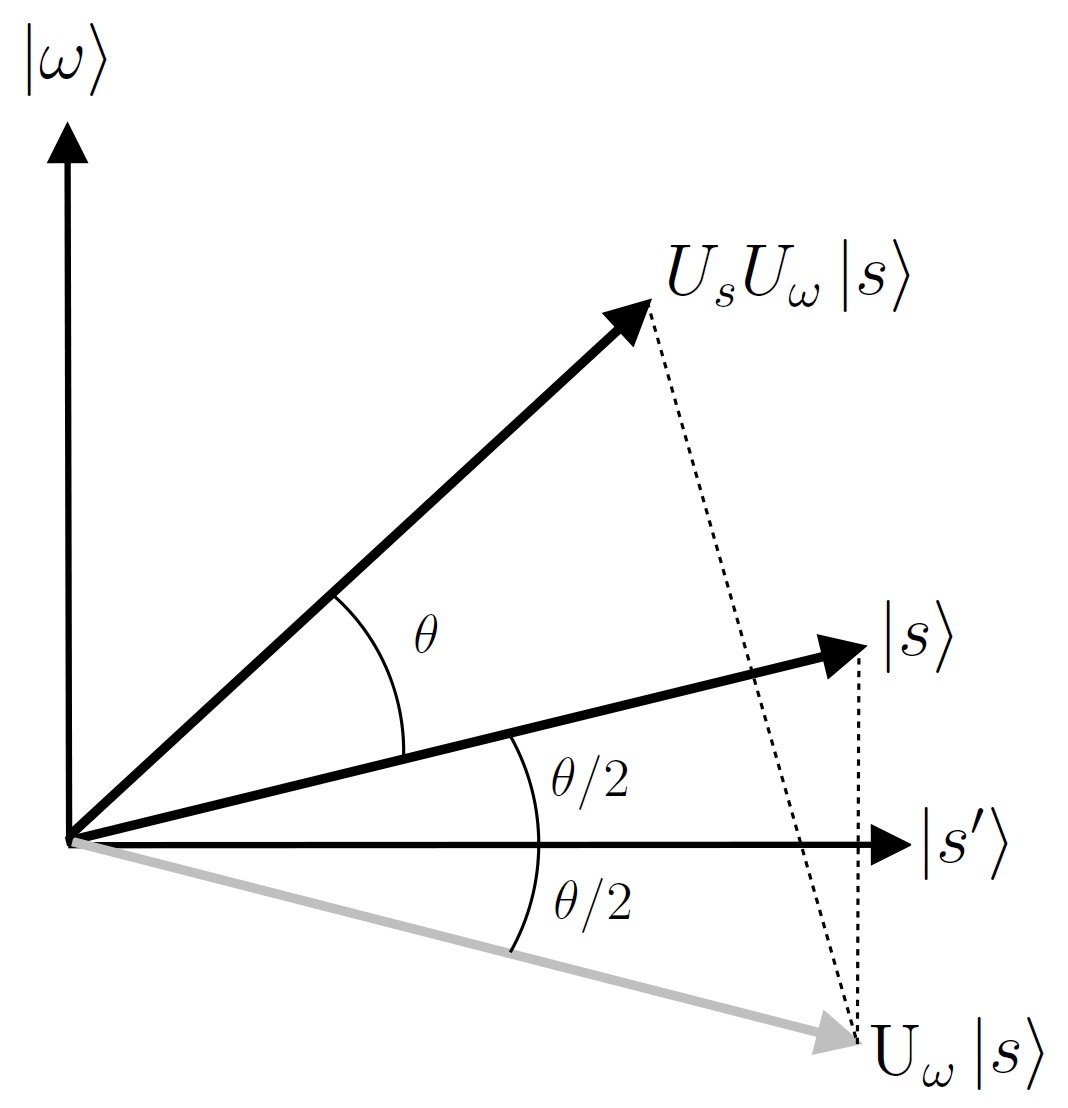
\includegraphics[width=0.3\linewidth]{img/grover_geometry.png}
\caption{Interpretación geométrica del operador difusión}
\end{figure}

\section{El algoritmo}

\begin{figure}[H]
\[ \Qcircuit @C=1.4em @R=1.8em {
\lstick{\ket{0}} & {/^n} \qw & \gate{H^{\otimes n}} & \gate{U_{\omega}} & \gate{U_s} & \meter & \cw \\
& & & \rstick{\hspace{-13pt} \lfloor\frac{\pi \sqrt{N}}{4}\rfloor \text{ veces}}
\gategroup{1}{4}{1}{5}{1.3em}{_\}}
} \]
\caption{Circuito del algoritmo de Grover.}
\end{figure}

\begin{enumerate}
    \item Preparar el estado fiducial.
    \item Aplicar la transformada de Walsh-Hadamard.
    \item Realizar la iteración de Grover $\lfloor \frac{\pi}{4} \sqrt{N} \rfloor$ veces.
    \begin{enumerate}
        \item Aplicar $U_{\omega}$.
        \item Aplicar $U_s$.
    \end{enumerate}
    \item Realizar la medida $\Omega$.
\end{enumerate}

\section{Variaciones y generalizaciones del algoritmo de Grover}

A continuación estudiaremos el algoritmo de amplificación de amplitud, el cual es una generalización del algoritmo de Grover para bases de datos con cualquier cantidad de estados objetivos, y el algoritmo de Grover en un paso, el cual es una variación del algoritmo de Grover en la que se mide en cada iteración.

\subsection{Algoritmo de amplificación de amplitud}

Esta generalización fue desarrollada independientemente por Brassar y H̨øyer en 1997 [ref] y por Grover en 1998 [ref]. Con este algoritmo se pueden utilizar funciones oráculo que marquen 1 para más de una entrada de la base de datos en la cual se realizará la búsqueda. Entonces, sea $\mathcal{W}$ el conjunto de entradas a encontrar, tenemos la función oráculo:

\begin{equation}
    f(x) =
    \begin{cases}
        1 & \text{si } x \in \mathcal{W} \\
        0 & \text{si } x \not\in \mathcal{W}
    \end{cases}
\end{equation}

Ahora sea el proyector $\Pi_\mathcal{W}$ tal que proyecte los estados del espacio de Hilbert $\mathcal{H}$ asociado a la base de datos en el espacio de Hilbert generado por los estados objetivos $\mathcal{H}_\mathcal{W}$:

\begin{equation}
    \Pi_\mathcal{W} = \sum\limits_k \ketbra{\omega_k}{\omega_k}
\end{equation}

Donde los estados $\ket{\omega_k}$ son los estados asociados a las entradas de la base de datos pertenecientes a $\mathcal{W}$.

Sea el estado inicial:

\begin{equation}
    \ket{\psi} = \sin(\theta) \ket{\psi_1} + \cos(\theta) \ket{\psi_0}
\end{equation}

Donde $\ket{\psi_1} = \frac{\Pi_\mathcal{W} \ket{\psi}}{\sin(\theta)}$ y $\sin(\theta) = \bra{\psi} \Pi_\mathcal{W} \ket{\psi}$. De aquí podemos hallar que $\ket{\psi_0} = \frac{(\mathds{1} - \Pi_\mathcal{W}) \ket{\psi}}{\cos(\theta)}$ y que $\cos(\theta) = \bra{\psi} (\mathds{1} - \Pi_\mathcal{W}) \ket{\psi}$.

Ahora definamos los siguientes operadores de reflexión $U_\psi = (2 \ketbra{\psi}{\psi}$ y $ U_\mathcal{W} = \mathds{1})(\mathds{1} - 2 \Pi_\mathcal{W})$, estos son las generalizaciones de $U_s$ y $U_\omega$, del algoritmo de Grover, respectivamente. El producto de ellos, $U_\psi U_\mathcal{W}$ es un operador de rotación en el plano generado por $\ket{\psi_0}$ y $\ket{\psi_1}$, de la misma manera que $U_s U_\omega$ es un operador de rotación en el plano generado por $\ket{s^\prime}$ y $\ket{\omega}$. Ahora veamos el efecto de $U_\psi U_\mathcal{W}$ y el ángulo que rota este operador:

\begin{multline}
    U_\psi U_\mathcal{W} \ket{\psi} = (2 \ketbra{\psi}{\psi} - \mathds{1}) (\mathds{1} - 2 \Pi_\mathcal{W}) \ket{\psi} = (2 \ketbra{\psi}{\psi} - \mathds{1}) [(\mathds{1} - \Pi_\mathcal{W}) - \Pi_\mathcal{W}] \ket{\psi} \\
    = (2 \ketbra{\psi}{\psi} - \mathds{1}) (\cos(\theta) \ket{\psi_0} - \sin(\theta) \ket{\psi_1}) = (2 \ketbra{\psi}{\psi} - \mathds{1}) (\ket{\psi} - 2 \sin(\theta) \ket{\psi_1}) \\
    = \ket{\psi} + (- 4 \sin^2(\theta) \ket{\psi} + 2 \sin(\theta) \ket{\psi_1}) = (3 - 4 \sin^2(\theta)) \sin(\theta) \ket{\psi_1} + (1 - 4 \sin^2(\theta)) \cos(\theta) \ket{\psi_0} \\
    = \sin(3 \theta) \ket{\psi_1} + \cos(3 \theta) \ket{\psi_0}
    \label{eq:DTheta}
\end{multline}

Como se puede ver, el operador $U_\psi U_\mathcal{W}$ rota un ángulo de $2 \theta$. Por lo que si se aplica $k$ veces a $\ket{\psi}$, tendremos:

\begin{equation}
    (U_\psi U_\mathcal{W})^k \ket{\psi} = \sin( (2 k + 1) \theta) \ket{\psi_1} + \cos( (2 k + 1) \theta) \ket{\psi_0}
\end{equation}

De esta manera, el $k = k_max$ para el cual se obtiene la probabilidad máxima de medir un elemento de $\mathcal{H}_\mathcal{W}$, es decir, el $k$ que maximiza la amplitud de probabilidad de la componente $\ket{\psi_1}$ de $\ket{\psi}$, es $\lfloor \frac{\pi}{4 \theta} \rfloor$. Así:

\begin{multline}
    (U_\psi U_\mathcal{W})^{k_{max}} \ket{\psi} = \sin( (2 \lfloor \frac{\pi}{4 \theta} \rfloor + 1) \theta) \ket{\psi_1} + \cos( (2 \lfloor \frac{\pi}{4 \theta} \rfloor + 1) \theta) \ket{\psi_0} \\
    \approx \sin(\frac{\pi}{2}) \ket{\psi_1} + \cos(\frac{\pi}{2}) \ket{\psi_0} = \ket{\psi_1}
\end{multline}

Mientras menor sea $\theta$, más tenderá $(U_\psi U_\mathcal{W})^{k_{max}} \ket{\psi}$ a $\ket{\psi_1}$, pero mayor será $k_{max}$.

Como se puede ver, el algoritmo de amplificación de amplitud se puede utilizar como algoritmo de búsqueda con una cantidad arbitraria de estados objetivos y un estado inicial arbitrario, no sólo $\ket{s}$ como en el algoritmo de Grover. Sin embargo, este no es sólo un algoritmo de búsqueda, sino tambien un algoritmo de optimización. En este sentido, la amplificación de amplitud también se puede utilizar como subrutina para mejorar el resultado de otros algoritmos. Sea $U_\mathcal{A}$ el operador asociado a un algoritmo cuántico $\mathcal{A}$, entonces, tal que, partiendo del estado fiducial, retorne el estado $\ket{\psi}$. Es decir, $U_\mathcal{A} \ket{0} = \ket{\psi}$, entonces, podemos reescribir $U_\psi$ de la siguiente manera:

\begin{equation}
    U_\psi = (2 \ketbra{\psi} - \mathds{1}) = (2 U_\mathcal{A} \ketbra{0} U_\mathcal{A}^\dagger - \mathds{1}) = U_\mathcal{A} (2 \ketbra{0} - \mathds{1}) U_\mathcal{A}^\dagger = U_\mathcal{A} U_0 U_\mathcal{A}^\dagger
\end{equation}

De esta manera, a cualquier algoritmo, que actúe sobre un espacio de Hilbert $\mathcal{H}$ que se pueda descomponer un espacio de estados buenos $\mathcal{H}_\mathcal{W}$ y un espacio de estados malos $\mathcal{H} \setminus \mathcal{H}_\mathcal{W}$, se le puede aplicar la amplificación de amplitud para mejorar su resultado.

Ahora consideremos el caso en el que $U_\mathcal{A} = H^{\otimes n}$, es decir, el caso en el que $\ket{\psi} = \ket{s}$. Este seria el caso particular del algoritmo de amplificación de amplitud en el que se utiliza el mismo estado inicial del algoritmo de Grover.

\begin{align}
    \ket{\psi} &= \frac{1}{\sqrt{N}} \sum\limits_i \ket{i} = \frac{1}{\sqrt{N}} \sum\limits_{i \in \mathcal{W}} \ket{i} + \frac{1}{\sqrt{N}} \sum\limits_{j \not\in \mathcal{W}} \ket{j} \\
    \ket{\psi_1} &= \frac{1}{\sqrt{W}} \sum\limits_{i \in \mathcal{W}} \ket{i} \\
    \sin{\theta} &= \sqrt{\frac{W}{N}} \\
    \ket{\psi_0} &= \frac{1}{\sqrt{N-W}} \sum\limits_{j \not\in \mathcal{W}} \ket{j} \\
    \cos{\theta} &= \sqrt{\frac{N-W}{N}}
\end{align}

Si tomamos $N \gg W$, tendríamos que $\theta \approx \sqrt{\frac{W}{N}}$, entonces $k_{max} \approx \frac{\pi}{4} \sqrt{\frac{N}{W}}$. Es interesante notar que mientras más estados buenos haya, menos iteraciones se necesitan. Pero a cambio, para hallar todos esos estados buenos, se debe ejecutar el algoritmo más veces. En caso de que $\mathcal{W}$ sea de dimensión 1, se recuperaría exactamente el algoritmo de Grover.

\subsection{Algoritmo de Grover en un paso}

En [ref] Grover propone una manera alternativa para ejecutar su algoritmo. En lugar de realizar $O(\sqrt{N})$ iteraciones, propone realizar una sola iteración en $\Omega(\sqrt{N \log(N)})$ sistemas identicos simultáneamente. Partiendo de la ecuación \ref{eq:prob1step}, la probabilidad de medir cada uno de los estados, cuando N es grande, luego de aplicar una iteración del algoritmo de Grover es aproximadamente:

\begin{equation}
    p(x) \approx
    \begin{cases}
        \frac{9}{N} & \text{si } x = \omega \\
        \frac{1}{N} & \text{si } x \neq \omega
    \end{cases}
\end{equation}

Así que con $\eta$ sistemas se tendrá, en promedio $9 \eta/N \pm O(\sqrt{\eta/N})$ medidas del valor deseado y $\eta/N \pm O(\sqrt{\eta/N})$ medidas de cualquiera de cada uno de los otros estados. La idea es tener suficientes sistemas para poder elegir con seguridad el valor que más se repita como el valor deseado. Por el teorema del límite central, la probabilidad de que una variable particular se desvíe más de $\pm \gamma \sqrt{\eta/N}$ de su valor esperado es menor que $e^{- \Omega(\gamma^2)}$. De esta manera, si $\eta = \Omega(N \log(N))$, entonces, con una probabilidad cercana a 1, el valor deseado ocurrirá con mayor frecuencia que cualquiera de los otros $N-1$.

Este esquema también se puede aplicar al algoritmo de amplificación de amplitud, pero con una condición: Que la cantidad de estados marcados sea menor a $N/4$. Esto es porque no hay manera de diferenciar los $W$ estados deseados de los otros $N - W$. Entonces, si $W$ es cercano a $N/2$, resultará imposible identificar correctamente los estados deseados.

Es importante mencionar que aunque esta versión del algoritmo se pueda ejecutar con una sola iteración, resulta menos eficiente que el algoritmo de Grover tradicional. Esto es porque esas $\Omega(N \log(N))$ mediciones necesitarán ser procesadas para hallar los valores más frecuentes, lo cual tendrá una complejidad temporal del mismo orden $\Omega(N \log(N))$, la cual es mayor a la complejidad temporal $O(\sqrt{N}$ de la versión tradicional del algoritmo. De esta forma, la única verdadera ventaja de esta variacíón estaría en el caso en que se tengan sistemas con tiempos de vida tales que no permitan realizar las iteraciones necessarias para ejecutar la versión tradicional del algoritmo de Grover.

\subsection{Optimización del algoritmo de Grover}

En [ref] Garg y Pande proponen una optimización del algoritmo de Grover, mezclando el algoritmo de Grover tradicional y el algoritmo de Grover de un paso. La idea de ellos es ejecutar el algoritmo en múltiples sistemas idénticos, como en el algoritmo de un paso, pero realizar más de una iteración, como en el algoritmo tradicional. De esta manera, reducen la cantidad $\eta$ de sistemas necesarios y la cantidad $k$ de iteraciones necesarias. Ellos hayan que tomando $\eta = k$, entonces sólo se necestian $O(\sqrt[3]{N})$.

Partiendo de \ref{eq:sinTheta0} y \ref{eq:DTheta}, sabemos que en cada iteración de Grover, cuando $N$ es grande, se rota un ángulo de aproximadamente $2/\sqrt{N}$ y que el ángulo inicial es aproximadamente $1/\sqrt{N}$. Así que luego de $k$ iteraciones, se tendrá un ángulo de aproximadamente $(2k + 1)/\sqrt{N}$. Por lo tanto, la probabilidad de medir cada estado será:

\begin{equation}
    p(x) \approx
    \begin{cases}
        \frac{(2k + 1)^2}{N} & \text{si } x = \omega \\
        \frac{1}{N} & \text{si } x \neq \omega
    \end{cases}
\end{equation}

Si realizamos esto en $\eta$ sistemas idénticos, entonces, mediremos el valor deseado $\eta (2k + 1)^2 / N \pm O(\sqrt{\eta k^2/N})$ veces y cada otro estado $\eta / N \pm O(\sqrt{\eta k^2/N})$ veces. Si tomamos $\eta = k$, entonces, mediremos $\omega$ alrededor de $k (2k + 1)^2 / N \pm O(\sqrt{k^3/N})$ veces. Ahora, si tomamos $k$ en el orden de $O(\sqrt[3]{N})$, tendremos $\omega$ alrededor de $\sqrt[3]{N} ( 2 \sqrt[3]{N} + 1)^2 \pm O(1)$ veces. Como $N$ es grande, podemos hacer la aproximación $2 \sqrt[3]{N} + 1 \approx 2 \sqrt[3]{N}$ y entonces, tendremos $\omega$ alrededor de $4 \pm O(1)$ veces. Mientras que todos los otros valores ocurriran sólo $N^{-2/3} \pm O(1)$ veces cada uno. Así que, el estado medido con mayor frecuencia ha de ser, con seguridad, el estado deseado.

Finalmente, la parte cuántica de este algoritmo tiene una complejidad temporal de $O(\sqrt[3]{N})$ y el procesamiento posterior de las mediciones realizadas también tendrá una complejidad temporal de $O(\sqrt[3]{N}$, pues esta es la cantidad de datos a procesar. Por lo tanto, la complejidad total de este algoritmo es $O(\sqrt[3]{N}$, la cual es menor a $O(\sqrt{N})$ de la versión tradicional y a $\Omega(N \log(N))$ de la versión en un paso.

\section{Simulaciones}

Se realizaron simulaciones del algoritmo de Grover con $\ket{\omega} = \ket{0000}$, $\ket{\omega} = \ket{0110}$ y $\ket{\omega} = \ket{1111}$. También se realizon simulaciones del algoritmo de amplificación de amplitud con $\mathcal{W} = \{9, 13\} = \{1001_2, 1101_2 \}$ y $\mathcal{W} = \{4, 5, 12, 13\} = \{0100_2, 0101_2, 1100_2, 1101_2\}$.

Un conjunto de las simulaciones se ha realizado en Wolfram Mathematica, implementando los operadores, es decir $U_{\omega}$, $U_\mathcal{W}$, $U_s$ y la transformada de Hadamard, directamente, de manera matricial, de acuerdo a las definiciones dadas anteriormente. Otro conjunto de las simulaciones ha realizado en Python, definiendo todos los operadores y transformaciones en base a sus construcciones circuitales, a partir de las compuertas nativas de los transmones, resolviendo la ecuación maestra del sistema al aplicar cada compuerta nativa. Al primer conjunto lo llamaremos simulaciones matemáticas, y al segundo, simulaciones circuitales. El código todas las simulaciones de este capítulo se encuentra en el apéndice \ref{ch:grovercod}.

En el caso de la simulaciones matemáticas, sólo se ha simulado el caso sin relajación. Por otro lado, en el caso de la simulaciones circuitales, se ha simulado el sistema tanto sin relajación, como con relajación. En el caso del sistema con relajación, se ha utilizado la ecuación maestra de Lindblad con los operadores de colapso $\sigma_{-_i}$ y tasa de relajación $\gamma = 25KHz$.

Como el espacio de Hilbert del sistema en el que sea ejecutado el algoritmo es de 16 dimensiones, ya que es de cuatro qubits, se necesitan $\lfloor \frac{\pi \sqrt{16}}{4} \rfloor = 3$ iteraciones para tener la máxima probabilidad de medir el estado deseado. Sin embargo, la simulación se ha realizado con 7 iteraciones, para apreciar la naturaleza oscilatoria de este algoritmo. Recordemos que este algoritmo consiste en rotaciones en el espacio 2D generado por $\ket{\omega}$ y $\ket{s^\prime}$, es decir, que si se aplican más de 3 rotaciones, la probabilidad de éxito debería disminuir, hasta que el estado del sistema se alinee con $- \ket{s^\prime}$, volver a aumentar hasta llegar a $- \ket{\omega}$, disminuir hasta pasar por $\ket{s^\prime}$, pasar de nuevo por el estado inicial $\ket{s}$ y repetirse el ciclo. La hipotesis es que veremos aproximadamente un período de sinusoide muestreada, con alrededor de seis muestras por período, en la gráfica de la evolución de la probabilidad de medir $\ket{\omega}$, ya que si luego de tres iteraciones se llega al punto de probabilidad máxima, alrededor de la sexta iteración se debe llegar al punto de probabilidad mínima y en la séptima volvería a aumentar.

En la figura \ref{fig:groverlosslesscomp1111} se puede observar la gráfica de la evolución de la probabilidad de medir cada estado en cada iteración del algoritmo de Grover con $\ket{\omega} = \ket{1111}$. Como se puede observar, ambas figuras son bastante similares. La fidelidad entre los estados finales de ambas simulaciones es 0.999875. Además, se ha confirmado la hipotesis de que la evolución de la probabilidad de medir $\ket{1111}$ tiene forma sinusoidal.

\begin{figure}[H]
    \centering
    \begin{subfigure}[m]{0.49\textwidth}
        \centering
        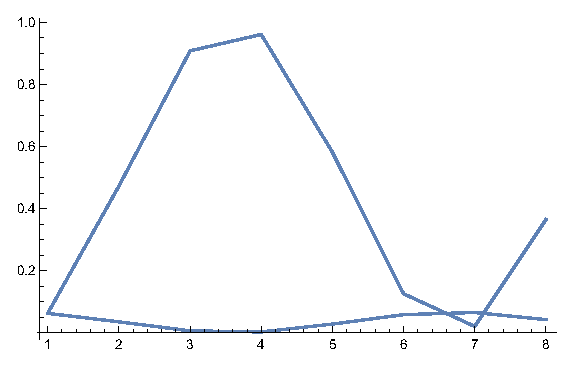
\includegraphics[width=0.9\linewidth]{img/Grover-2_gr1.eps}
        \caption{Wolfram Mathematica}
    \end{subfigure}
    \begin{subfigure}[m]{0.49\textwidth}
        \centering
        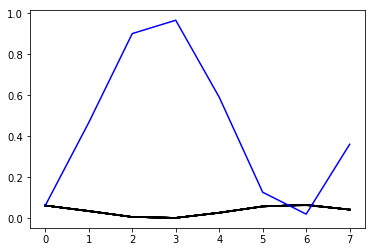
\includegraphics[width=0.9\linewidth]{img/groveralllossless.png}
        \caption{Python}
    \end{subfigure}
    \caption[Evolución de las probabilidades en el algoritmo de Grover sin relajación]{Evolución de las probabilidades en el algoritmo de Grover sin relajación}
    \label{fig:groverlosslesscomp1111}
\end{figure}

Ahora, compararemos los resultados de la simulación circuital con y sin relajación. Como se puede ver en la figura \ref{fig:groverlosscomp}, en el caso con relajación, los estados que no contienen el valor deseado dejan de tener todos la misma probabilidad. Los estados que involucran el estado base ganan probabilidad debido a la relajación de los qubits. La fidelidad entre los estados resultantes de los casos con y sin relajación es de 0.250818.

Además, en el caso con relajación, la probabilidad de medir el estado deseado depende de cuál sea este estado. Mientras más particiones en $\ket{1}$ contenga este estado, peor será el efecto de la relajación en el algoritmo. Esto ocurre porque el algoritmo debe llevar estas particiones a estado excitados, es decir, a estados de energías superiores y esto es energía que el entorno absorbe por efecto Purcell. Las particiones en el estado $\ket{0}$ están en su estado base y no se ven afectadas por este fenómeno, pues este es su estado de mínima energía. Esto se ve reflejado en las siguientes figuras.

En la figura \ref{fig:groverlosscomp}, se tiene $\ket{\omega} = \ket{1111}$, así que este es el caso en el que el entorno tiene el mayor efecto sobre el algoritmo, pues es el caso en el que el sistema tiene las mayores energías. Por otro lado, la figura \ref{fig:groverloss0000} presenta el caso en el que $\ket{\omega} = \ket{0000}$, este es el caso en el que el entorno tiene el menor efecto sobre el algoritmo, pues es el caso en el que el sistema tiene las menores energías. La figura \ref{fig:groverloss0110} presenta el caso en el $\ket{\omega} = \ket{0110}$. Este es un caso intermedio y el sistema tiene un efecto distinto sobre cada partición.

\color{red}Los tiempos de vida no son suficientes\color{black}

\begin{figure}[H]
    \centering
    \begin{subfigure}[m]{0.49\textwidth}
        \centering
        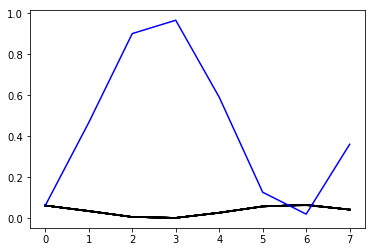
\includegraphics[width=0.99\linewidth]{img/groveralllossless.png}
        \caption{Sin relajación}
    \end{subfigure}
    \begin{subfigure}[m]{0.49\textwidth}
        \centering
        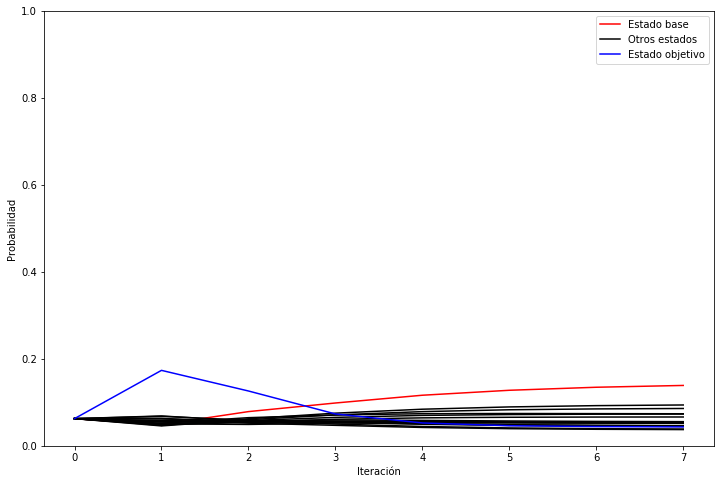
\includegraphics[width=0.99\linewidth]{img/groverallloss.png}
        \caption{Con relajación}
    \end{subfigure}
    \caption[Evolución de las probabilidades en el algoritmo de Grover con relajación, $\mathcal{W} = \{15\}$]{Evolución de las probabilidades en el algoritmo de Grover con relajación, $\mathcal{W} = \{15\} \{1111_2\}$}
    \label{fig:groverlosscomp}
\end{figure}

\begin{figure}[H]
    \centering
    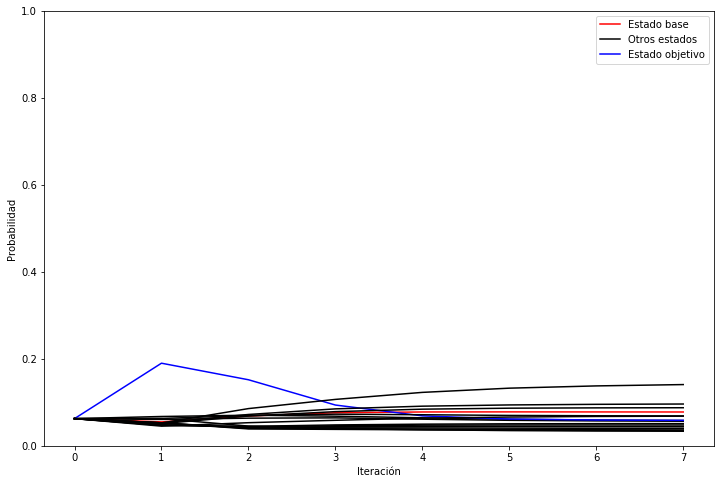
\includegraphics[width=0.75\linewidth]{img/grover0110loss.png}
    \caption[Evolución de las probabilidades en el algoritmo de Grover con relajación, $\mathcal{W} = \{6\}$]{Evolución de las probabilidades en el algoritmo de Grover con relajación, $\mathcal{W} = \{6\} = \{0110_2\}$}
    \label{fig:groverloss0110}
\end{figure}

\begin{figure}[H]
    \centering
    \begin{subfigure}[m]{0.49\textwidth}
        \centering
        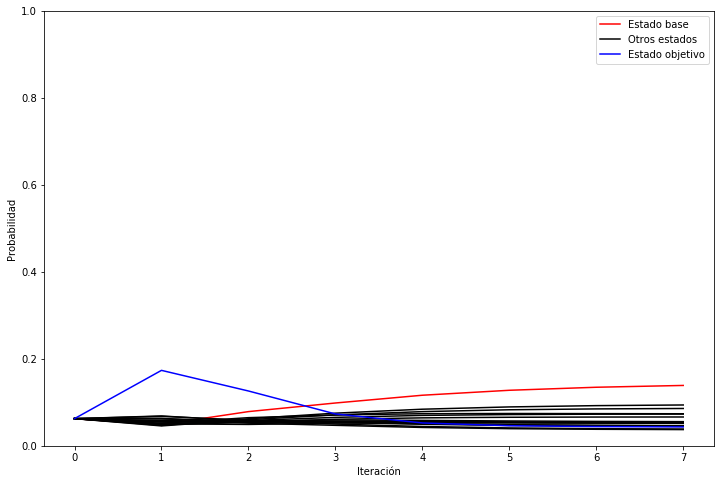
\includegraphics[width=0.99\linewidth]{img/groverallloss.png}
        \caption{$\omega = 15$}
    \end{subfigure}
    \begin{subfigure}[m]{0.49\textwidth}
        \centering
        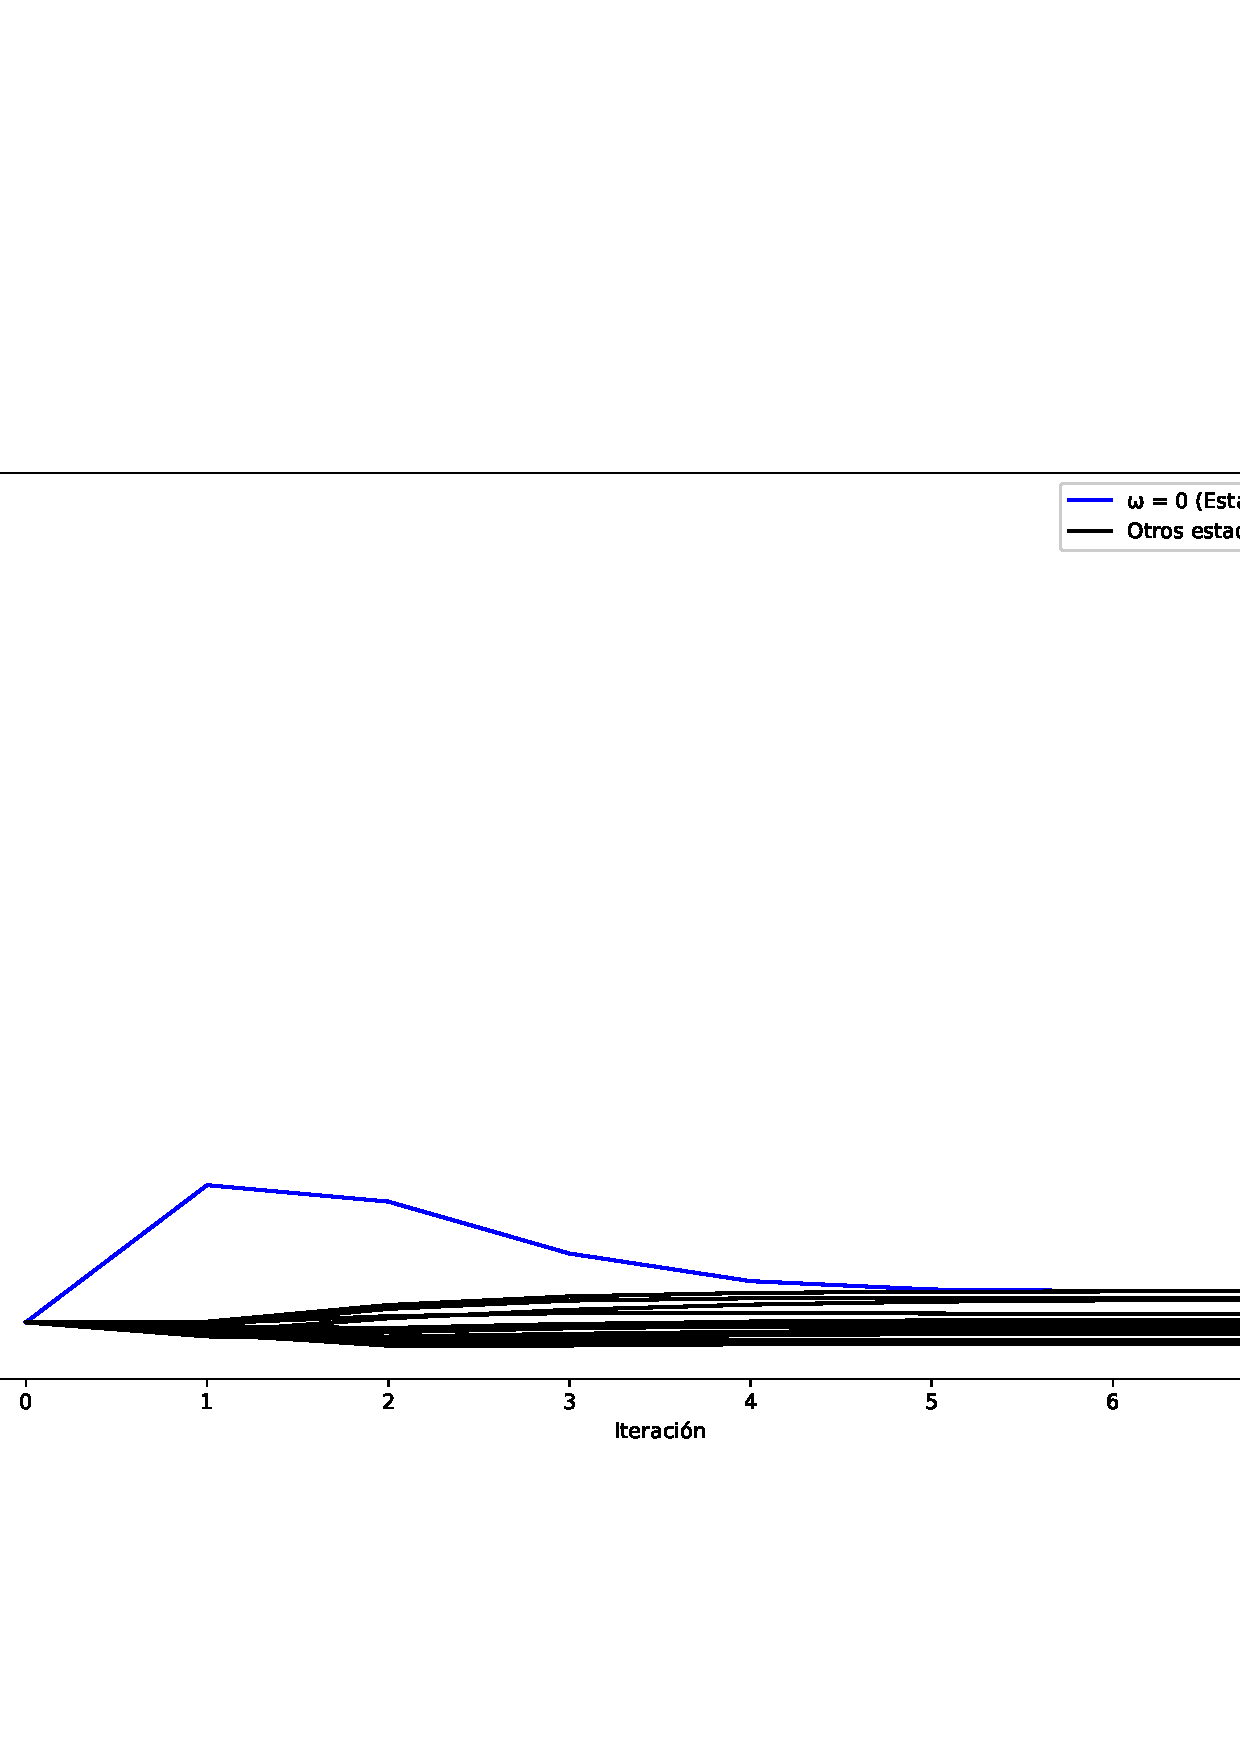
\includegraphics[width=0.99\linewidth]{img/grover0000loss.png}
        \caption{$\omega = 0$}
    \end{subfigure}
    \caption[Evolución de las probabilidades en el algoritmo de Grover con relajación, $\mathcal{W} = \{0\}$]{Evolución de las probabilidades en el algoritmo de Grover con relajación, $\mathcal{W} = \{0\} = \{0000_2\}$}
    \label{fig:groverloss0000}
\end{figure}

Ahora veamos los casos en los que se tiene más de un estado deseado

\begin{figure}[H]
    \centering
    \begin{subfigure}[m]{0.49\textwidth}
        \centering
        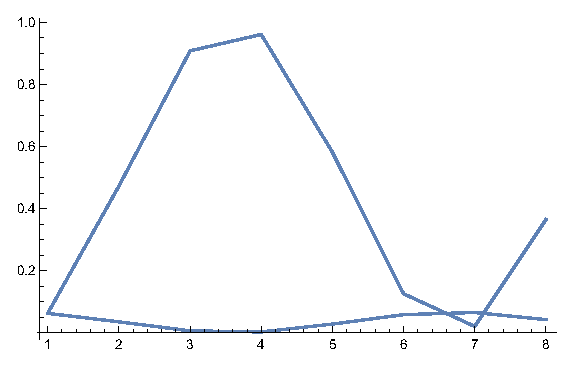
\includegraphics[width=0.9\linewidth]{img/Grover-2_gr1.eps}
        \caption{Wolfram Mathematica}
    \end{subfigure}
    \begin{subfigure}[m]{0.49\textwidth}
        \centering
        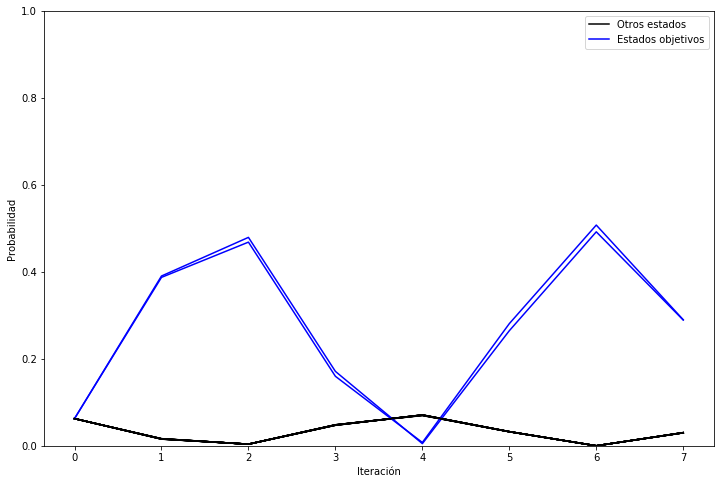
\includegraphics[width=0.9\linewidth]{img/grover2lossless.png}
        \caption{Python}
    \end{subfigure}
    \caption[Evolución de las probabilidades en el algoritmo de Grover sin relajación $\mathcal{W} = \{9, 13\}$]{Evolución de las probabilidades en el algoritmo de Grover sin relajación $\mathcal{W} = \{9, 13\} = \{1001_2, 1101_2\}$}
    \label{fig:groverlosslesscomp2}
\end{figure}

\begin{figure}[H]
    \centering
    \begin{subfigure}[m]{0.49\textwidth}
        \centering
        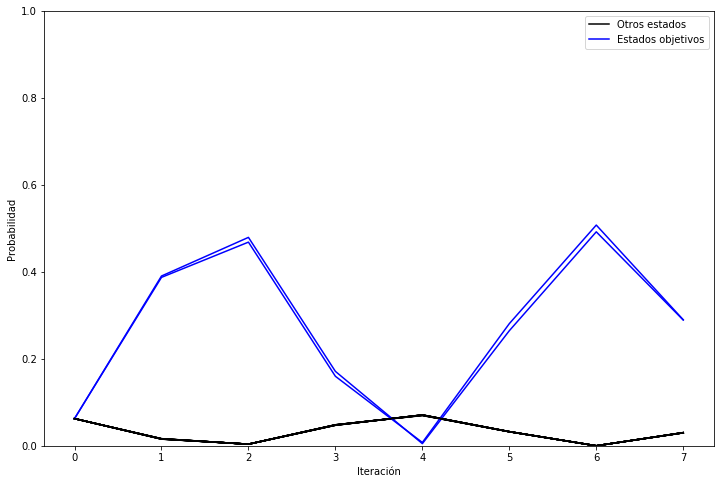
\includegraphics[width=0.99\linewidth]{img/grover2lossless.png}
        \caption{Sin relajación}
    \end{subfigure}
    \begin{subfigure}[m]{0.49\textwidth}
        \centering
        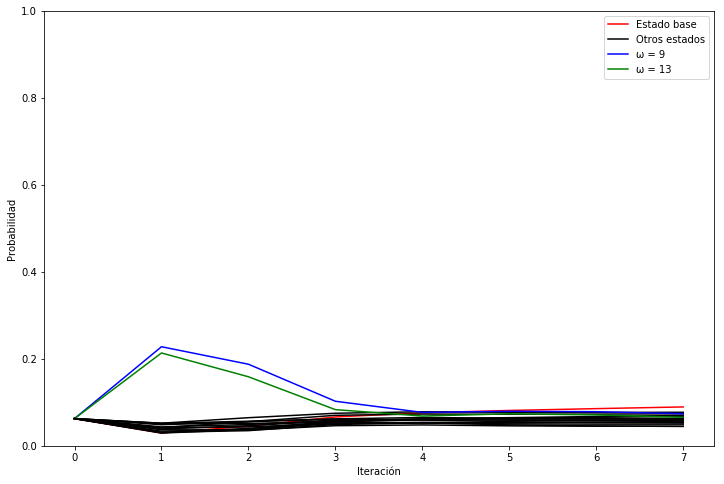
\includegraphics[width=0.99\linewidth]{img/grover2loss.png}
        \caption{Con relajación}
    \end{subfigure}
    \caption[Evolución de las probabilidades en el algoritmo de Grover sin relajación, $\mathcal{W} = \{9, 13\}$]{Evolución de las probabilidades en el algoritmo de Grover sin relajación $\mathcal{W} = \{9, 13\} = \{1001_2, 1101_2\}$}
    \label{fig:groverlosscomp2}
\end{figure}


\begin{figure}[H]
    \centering
    \begin{subfigure}[m]{0.49\textwidth}
        \centering
        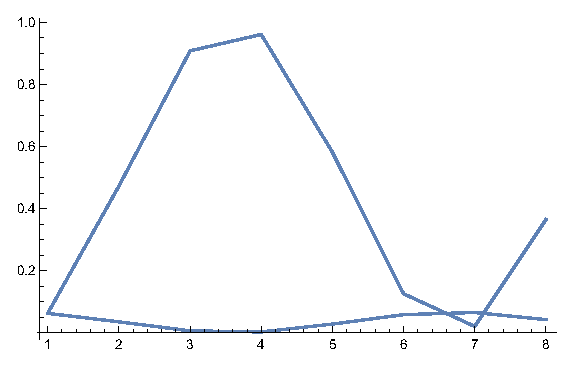
\includegraphics[width=0.9\linewidth]{img/Grover-2_gr1.eps}
        \caption{Wolfram Mathematica}
    \end{subfigure}
    \begin{subfigure}[m]{0.49\textwidth}
        \centering
        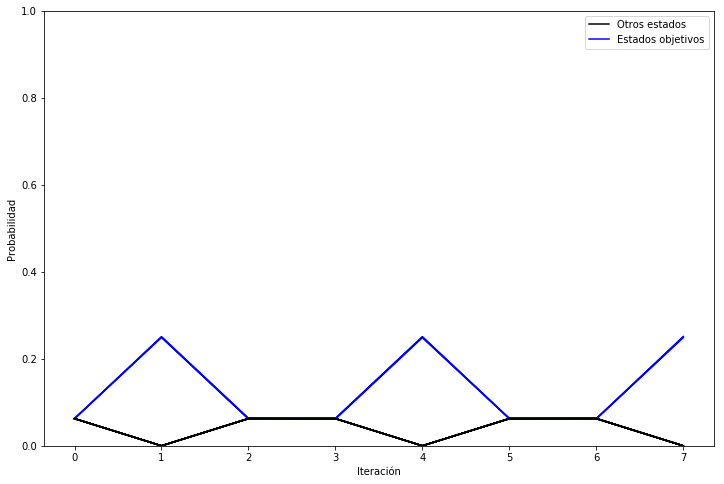
\includegraphics[width=0.9\linewidth]{img/grover3lossless.png}
        \caption{Python}
    \end{subfigure}
    \caption[Evolución de las probabilidades en el algoritmo de Grover sin relajación $\mathcal{W} = \{4, 5, 12, 13\}$]{Evolución de las probabilidades en el algoritmo de Grover sin relajación $\mathcal{W} = \{4, 5, 12, 13\} = \{0100_2, 0101_2, 1100_2, 1101_2\}$}
    \label{fig:groverlosslesscomp3}
\end{figure}

\begin{figure}[H]
    \centering
    \begin{subfigure}[m]{0.49\textwidth}
        \centering
        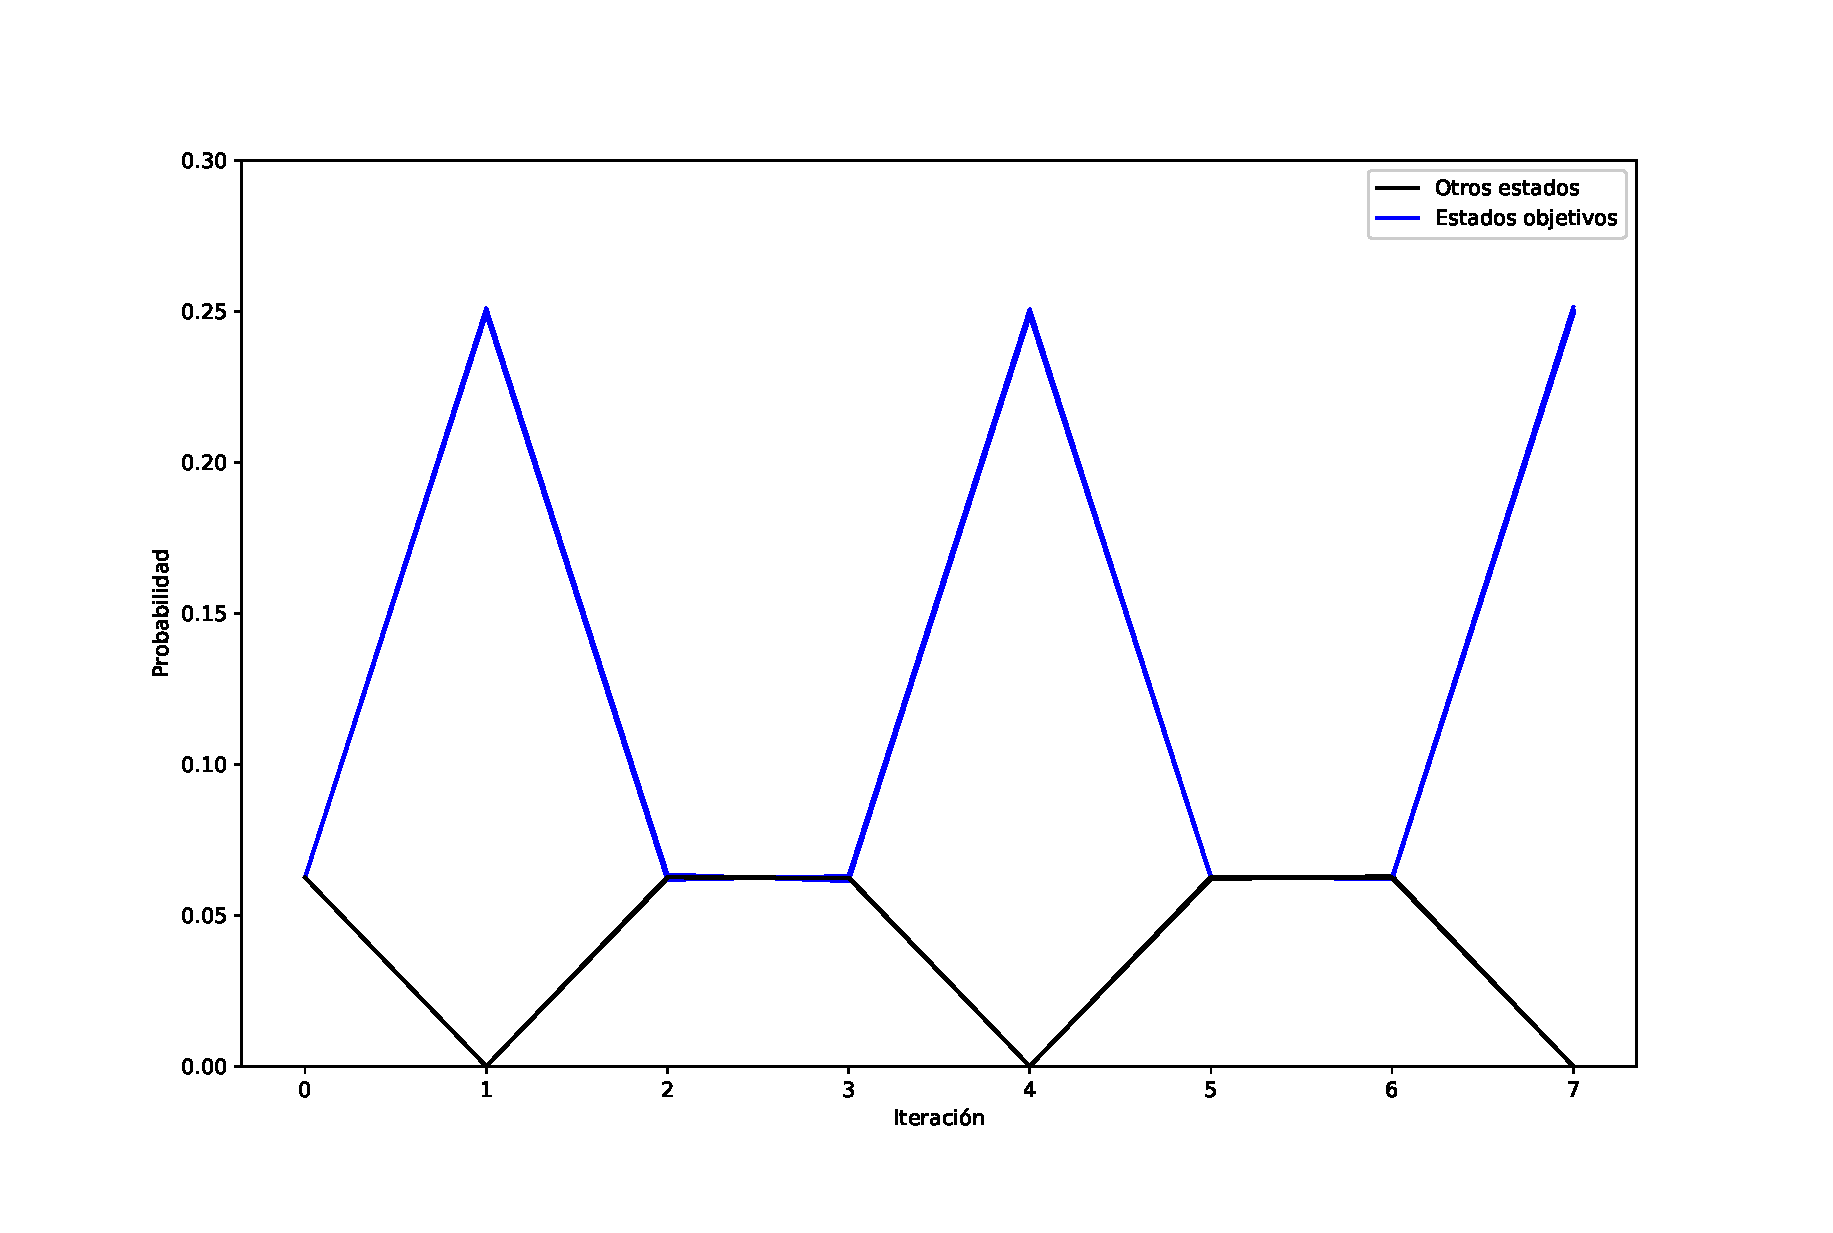
\includegraphics[width=0.99\linewidth]{img/grover3lossless.eps}
        \caption{Sin relajación}
    \end{subfigure}
    \begin{subfigure}[m]{0.49\textwidth}
        \centering
        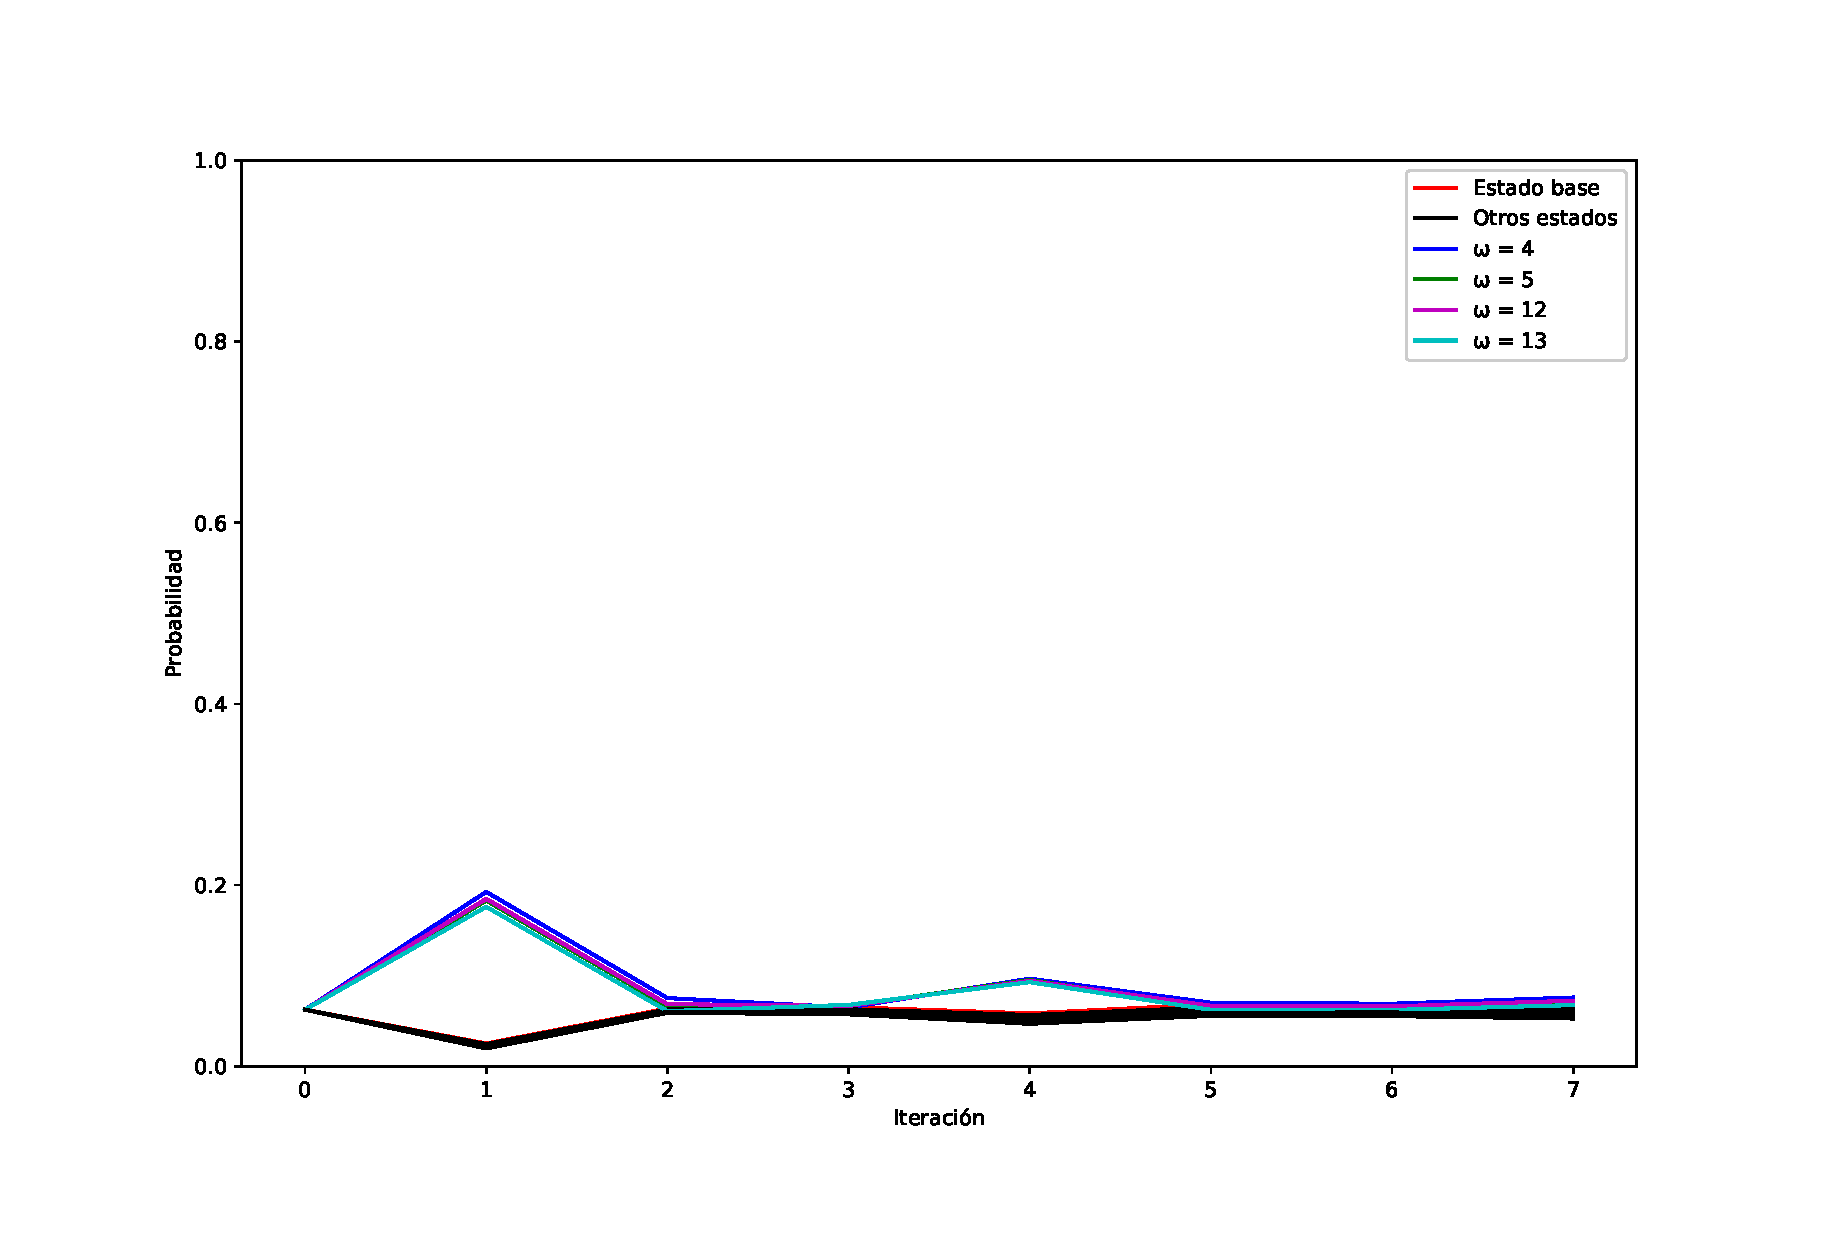
\includegraphics[width=0.99\linewidth]{img/grover3loss.eps}
        \caption{Con relajación}
    \end{subfigure}
    \caption[Evolución de las probabilidades en el algoritmo de Grover con relajación $\mathcal{W} = \{4, 5, 12, 13\}$]{Evolución de las probabilidades en el algoritmo de Grover con relajación $\mathcal{W} = \{4, 5, 12, 13\} = \{0100_2, 0101_2, 1100_2, 1101_2\}$}
    \label{fig:groverlosscomp3}
\end{figure}


\subsection{Algoritmo de Grover en un paso y optimización}




\chapter{Algoritmo de Shor}
El algoritmo de Shor es un AC de factorización de enteros. Dado un entero $N=p \times q$, donde $p$ y $q$ son primos, el algoritmo de Shor encuentra $p$ y $q$ en $O((\log(N))^3)$ pasos. El algoritmo clásico más eficiente para factorizar enteros es la cibra general del cuerpo de números y funciona con una complejidad heurística de $O(e^{(\sqrt[3]{\frac{64}{9}}+o(1))(\ln(N))^{\frac{1}{3}}(\ln(\ln(N)))^{\frac{2}{3}}})$. Por su capacidad de factorizar números semiprimos, el algoritmo de Shor es capaz de violar el cifrado RSA y el protocolo Diffie-Hellman de intercambio de llaves, sobre los cuáles se basa virtualmente toda la criptografía actual.

El algoritmo de Shor requiere de dos algoritmos cuánticos preliminares: La estimación de fase y la estimación de orden. El algoritmo de estimación de fase permite encontrar la fase $\phi$ del autovalor $e^i \phi$ asociado a algún autoestado $\ket{u}$ de un operador unitario U. El algoritmo de estimación de orden se basa en la estimación de fase para hallar el orden $r>0$ tal que $a^r \equiv 1 \mod m$.

\section{Transformada cuántica de Fourier}

Una de las transformadas integrales cuánticas más importantes es la tranformada cuántica de Fourier. Sea $\omega_n$ la n-ésima raíz primitiva de la unidad:

\begin{equation}
    \omega_n = e^{2\pi i/N}
\end{equation}

Donde $N = 2^n$. El número complejo $\omega_n$ define el kernel K como:

\begin{equation}
    K(x,y) = \frac{1}{\sqrt{N}} \omega_n^{x y}
\end{equation}

La transformada integral discreta con el kernel K,

\begin{equation}
    \tilde{f}(y) = \frac{1}{\sqrt{N}} \sum\limits_x \omega^{-x y} f(x)
\end{equation}

se llama la transformada discreta de Fourier (DFT).

El kernel K es unitario ya que:

\begin{multline}
    (K K^\dagger)(x,y) = \bra{x} K K^\dagger \ket{y}
    = \bra{x} K \sum\limits_z \ketbra{z}{z} K^\dagger \ket{y} \\
    = \sum\limits_z K(x,z) K^\dagger(z,y) 
    = \frac{1}{N} \sum\limits_z \omega^{-x z} \omega^{y z} 
    = \frac{1}{N} \sum\limits_z \omega^{- (z-y) z} 
    = \delta_{x y}
\end{multline}

La transformada integral cuántica definida con este kernel se llama transformada cuántica de Fourier.

El kernel para $n = 1$ es:

\begin{equation}
    K_1 = \frac{1}{\sqrt{2}}
    \begin{pmatrix}
        1 & 1 \\
        1 & e^{2\pi i/2}
    \end{pmatrix} =
    \frac{1}{\sqrt{2}}
    \begin{pmatrix}
        1 & 1 \\
        1 & -1
    \end{pmatrix}
\end{equation}

El cual no es más que la compuerta de Hadamard. Para $n = 2$, tenemos $\omega_2 = e^{2\pi i/4} = i$ y:

\begin{equation}
    K_2 = \frac{1}{2}
    \begin{pmatrix}
        1 & 1 & 1 & 1 \\
        1 & \omega_2^{-1} & \omega_2^{-2} & \omega_2^{-3} \\
        1 & \omega_2^{-2} & \omega_2^{-4} & \omega_2^{-6} \\
        1 & \omega_2^{-3} & \omega_2^{-6} & \omega_2^{-9}
    \end{pmatrix} =
    \frac{1}{2}
    \begin{pmatrix}
        1 & 1 & 1 & 1 \\
        1 & -i & -1 & i \\
        1 & -1 & 1 & -1 \\
        1 & i & -1 & -i
    \end{pmatrix}
\end{equation}

La QFT inversa está dada por:

\begin{equation}
    QFT^{-1} = QFT^\dagger = \frac{1}{\sqrt{N}} \sum\limits_x\sum\limits_k e^{- 2\pi i k x / N} \ketbra{x}{k}
\end{equation}

\section{Estimación de fase}

Asumamos que tenemos un operador U, con autoestados $\ket{u}$ de dimensión L, y con autovalore complejos desconocidos $\lambda_\phi = e^{2 i \pi \phi}$, donde $\phi$ es un número real tal que $0 \leq \phi \leq 1$, a ser determinado.

Asumamos también que somos capaces de construir una familia de operadores $CU^p$, donde $p = 2^0, 2^1, 2^2, ..., 2^{k-1}$

El circuito cuántico del algoritmo de estimación de fase viene expresado en dos etapas, a las que llamaremos ``front-end'' y ``back-end''.

\[\Qcircuit @C=1.4em @R=1.8em {
\lstick{\ket{0}^{\otimes K}}& {/^K}\qw & \gate{H^{\otimes K}} & \ctrl{1}   & \gate{QFT^\dagger} & \meter & \cw \\
\lstick{\ket{u} \quad}      & {/^L}\qw & \qw                  & \gate{U^j} & \qw                & \qw    & \qw \\
& \rstick{\hspace{10pt} \text{Front-end}} & & & \rstick{\hspace{-10pt} \text{Back-end}}
\gategroup{1}{2}{2}{4}{1em}{_\}}
\gategroup{1}{5}{2}{6}{2.45em}{_\}}
} 
\]

Analicemos la etapa front-end:

\[\Qcircuit @C=1.4em @R=1.8em {
\lstick{\ket{0}} & \gate{H}  & \qw            & \qw            & \qw            & \ctrl{4}       & \qw \\
\lstick{\ket{0}} & \gate{H}  & \qw            & \qw            & \ctrl{3}       & \qw            & \qw \\
\lstick{\ket{0}} & \gate{H}  & \qw            & \ctrl{2}       & \qw            & \qw            & \qw \\
\lstick{\ket{0}} & \gate{H}  & \ctrl{1}       & \qw            & \qw            & \qw            & \qw \\
\lstick{\ket{u}} & {/^L} \qw & \gate{U^{2^0}} & \gate{U^{2^1}} & \gate{U^{2^2}} & \gate{U^{2^3}} & \qw \\
} 
\]

El circuito consta de dos registros. El primer registro empieza con el estado $\ket{0}$, mientras que el segundo empieza con un autoestado $\ket{u}$. Se aplica la transformada de Hadamard al primer registro para convertirlo en $\ket{s}$. Ahora se aplica U controlado por cada uno de los qubits del primer registro, como se ve en el circuito, tal que se aplique la fase del autovalor asociado a $\ket{u}$ n veces al estado $\ket{n}$. Para ilustrar mejor esto, veamos el efecto de $CU^j$ en distintos estados.

$\ket{0} = \ket{0000}:$

Como este estado está compuesto de sólo qubits $\ket{0}$, $CU^j$ actúa como $\mathds{1}$ y el estado de salida es igual al de entrada.

\begin{equation}
    CU^j \ket{0000} \otimes \ket{u} = e^{i 0 \times 2\pi \phi} \ket{0} \otimes \ket{u}
\end{equation}

$\ket{1} = \ket{0001}:$

La última partición de este estado es $\ket{1}$, así que la componente $CU^{2^0} = CU$ de $CU^j$ actúa como $U$, por lo tanto, aparece una vez la fase del autovalor $e^{i 2\pi \phi}$.

\begin{equation}
    CU^j \ket{0001} \otimes \ket{u} = e^{i 1 \times 2\pi \phi} \ket{1} \otimes \ket{u}
\end{equation}

$\ket{6} = \ket{0110}:$

La segunda y la tercera partición de este estado son $\ket{1}$, así que las componentes $CU^{2^1} = CU^2$ y $CU^{2^2} = CU^4$ de $CU^j$ actúan como $U^2$ y $U^4$. En total se tiene $U^6$, por lo tanto, aparece seis vez la fase del autovalor $e^{i 2\pi \phi}$.

\begin{equation}
    CU^j \ket{0110} \otimes \ket{u} = e^{i 6 \times 2\pi \phi} \ket{6} \otimes \ket{u}
\end{equation}

Como se puede ver, $CU^j \ket{n} \otimes \ket{u} = e^{i n 2\pi \phi} \ket{n} \otimes \ket{u}$. Por lo tanto, como las compuertas cuánticas son operadores lineales, sabemos que

\begin{equation}
    CU^j \ket{s} \otimes \ket{u} = CU^j \frac{1}{\sqrt{2^K}} \sum\limits_k \ket{k} \otimes \ket{u} = \frac{1}{\sqrt{2^K}} \sum\limits_k e^{i k 2\pi \phi} \ket{k} \otimes \ket{u}
\end{equation}

Ahora, se aplica la transformada cuántica inversa de Fourier al primer registro.

\begin{equation}
    QFT^\dagger = \frac{1}{\sqrt{2^K}} \sum\limits_x\sum\limits_k e^{-i 2\pi k x / 2^K} \ketbra{x}{k}
\end{equation}

\begin{equation}
\begin{array}{r l}
    QFT^\dagger \frac{1}{\sqrt{2^K}} \sum\limits_k e^{i k 2\pi \phi} \ket{k} \otimes \ket{u} &= \frac{1}{2^K} \sum\limits_x \sum\limits_k e^{i k 2\pi \phi} e^{-i 2\pi k x / 2^K} \ket{x} \otimes \ket{u} \\
    &= \frac{1}{2^K} \sum\limits_x\sum\limits_k \left(e^{i 2\pi (\phi - \frac{x}{2^K})}\right)^k \ket{x} \otimes \ket{\phi} \\
    &= \frac{1}{2^K} \sum\limits_x \frac{1 - e^{i 2\pi (\phi - \frac{x}{2^K}) 2^K}}{1 - e^{i 2\pi (\phi - \frac{x}{2^K})}} \ket{x} \otimes \ket{\phi} \\
\end{array}
\end{equation}

La probabilidad de medir x a la salida del registro será:

\begin{equation}
    p(x) = \frac{1}{4^{K}} \frac{\sin^2(\pi (\phi - \frac{x}{2^K}) 2^K)}{\sin^2(\pi (\phi - \frac{x}{2^K}))}
\end{equation}

$p(n) = |\bra{u} \otimes \bra{n} \ket{\psi_{output}}|^2$

$p(n) = \frac{1}{N^2} |\frac{1 - e^{2 i \pi (\phi - \frac{n}{N})N}}{1 - e^{2 i \pi (\phi - \frac{n}{N})}}|^2$

$\therefore p(n) = \frac{1}{N^2} \frac{\sin^2(\pi (\phi - \frac{n}{N}) N)}{\sin^2(\pi (\phi - \frac{n}{N}))}$

La medida de n con probabilidad asociada p(n), corresponde a la estimación de fase $\tilde{\phi} = n/N$. La probabilidad es máxima cuando $\delta = \phi - \tilde{\phi}$ es mínima.

$p(n) = \frac{1}{N^2} \frac{\sin^2(\pi (\phi - \frac{n}{N}) N)}{\sin^2(\pi (\phi - \frac{n}{N}))}$ si N es grande $\rightarrow$ %Graf

La probabilidad p(n) decae rápidamente a cero cuando el error $\delta$ se aleja del mínimo.

Entonces:

.) La medida tiene la maor probabilidad de dar la aproximación más cercana al estado $\phi$.
.) El circuito de salida es de la forma $\ket{\tilde{\phi}} \ket{u}$, donde $\ket{\tilde{\phi}}$ es una superposición de estados, los cuales al medirlos dan una buena aproximación de $\phi$.

\section{Estimación de orden}

Dado $m \in \mathds{N}$, se dice que $a,b \in \mathds{Z}$ son congruentes módulo m si y sólo si $(a-b)/m \in \mathds{Z}$.

\begin{enumerate}
    \item Se denota por $a \equiv b \mod m$, siendo m el módulo de la congruencia.
    \item Si m divide a $(a-b)$, ambos a y b tienen el mismo resto al ser divididos por el módulo m.
\end{enumerate}

 Ejemplos:

\begin{align*}
    23 \equiv 2 \mod 7 &\rightarrow 23 = 3 \times 7 + 2 \\
    -6 \equiv 1 \mod 7 &\rightarrow -6 = -1 \times 7 +1
\end{align*}

 Además si $m \in \mathds{N}$ y $a,b,c,d \in \mathds{Z}$ tales que:

\begin{align*}
    a+c &\equiv b+d \mod m \\
    a c &\equiv b d \mod m
\end{align*}

 Por definición el orden de $x \mod N$ es el menor entero r distinto de cero que satisface $x^r = 1 \mod N$
 
Ejemplo:

 Sea $x = 4, N = 13 \rightarrow 4^p = 13 q + R \qquad 4^p \mod 13 = R$

 \[\begin{matrix}
         p  &   4^p & 4^p = 13 q                         + R    &   R   \\
         0  &   1   & 4^0 = 13\times0                    + 1    & 1     \\
         1  &   4   & 4^1 = 13\times0                    + 4    & 4     \\
         2  &   16  & 4^2 = 13\times1                    + 3    & 3     \\
         3  &   64  & 4^3 = 13\times4                    + 12   & 12    \\
         4  &   256  & 4^4 = 13\times19                  + 9    & 9     \\
         5  &   1024  & 4^5 = 13\times78                 + 10   & 10    \\ % Revisar tabla | Error en la clase
         6  &   4096  & 4^6 = 13\times315                + 1    & 1     \\
         7  &   16384  & 4^7 = 13\times1260              + 4    & 4     \\
         8  &   65536  & 4^8 = 13\times5041              + 3    & 3     \\
         9  &   262144  & 4^9 = 13\times20164            + 12   & 12    \\
         10 &   1048576  & 4^10 = 13\times80659          + 9    & 9     \\
         11 &   4194304  & 4^11 = 13\times322638         + 10   & 10    \\
         12 &   16777216  & 4^12 = 13\times1290555       + 1    & 1     \\
         13 &   67108864  & 4^13 = 13\times5162220       + 4    & 4     \\
         14 &   268435456  & 4^14 = 13\times20648881     + 3    & 3     \\
         15 &   1073741824  & 4^15 = 13\times82595524    + 12   & 12    \\
         16 &   4294967296  & 4^16 = 13\times330382099   + 9    & 9     
     \end{matrix}
 \]

 Como podemos ver el período es r=6, el cual corresponde al menor r entero distinto de cero para el cual se cumple $4^r=1 \mod 13$ con r=6

 $\therefore 4^6 = 1 \mod 13$

Analicemos como la estimación de fase hace posible determinar r, el orden de $x \mod N$, con alta probabilidad y precisión. Primero necesitamos introducir el operador U y sus correspondientes autovectores y autovalores.

Asumamos que dados dos enteros x y N que satisfacen que $x<N$, siendo x coprimo de M, es decir mcd(x,M)=1, existe un operador $U_{x,N}$ tal que:

\begin{equation}
    U_{x,N} \ket{y} = \ket{x y \mod N}
\end{equation}

Sea $\{ \ket{u_s}\}_{s = 0, 1, ..., r-1}$ el conjunto de r autoestados de U, asociados con los autovalores $e^{i 2 \pi s/r}$ tal que $U \ket{u_s} = e^{2 i \pi s /r} \ket{u_s}$ en el cual la fase es $\phi_s = s/r$ con $0 \leq \phi_s \leq 1$

Tales autoestados $\ket{u_s}$ se definen acorde a: $\ket{u_s} = \frac{1}{\sqrt{r}} \sum\limits_{k=0}^{r-1} e^{\frac{-2 i \pi k s}{r}} \ket{x^k \mod N}$, siendo r a determinar.

Con las siguientes propiedades:

\begin{enumerate}
    \item $\frac{1}{\sqrt{r}} \sum_{s=0}{r-1} \ket{u_s} = \ket{1}$
    \item $\frac{1}{\sqrt{r}} \sum\limits_{s=0}^{r-1} e^{\frac{2 i \pi k s}{r}} \ket{u_s} = \ket{x^k \mod N}$
    \item $p(s) = |c_s|^2 = \frac{1}{r}$
\end{enumerate}

Entonces:

\begin{equation}
    CU^j \ket{j} \otimes \ket{1} = \ket{j} \otimes \ket{x^j \mod N}
\end{equation}

Con este paso entendido vamos ahora a analizar el circuito para determinar el orden:

\begin{enumerate}
    \item $\ket{\psi_1} = \ket{0}^{\otimes k} \otimes \ket{1}$
    \item $\ket{\psi_2} = \frac{1}{\sqrt{M}} (\ket{0} + \ket{1})^{\otimes k} \otimes \ket{1}; M=2^k$
        \begin{equation}
            \ket{\psi_2} = \frac{1}{\sqrt{M}} \sum_{j=0}^{M-1} CU^j (\ket{j} \otimes \ket{1})
        \end{equation}
    \item $\ket{\psi_3} = CU^j \ket{\psi_2} = \frac{1}{\sqrt{M}} \sum\limits_{j=0}^{M-1} CU^j (\ket{j} \otimes \ket{1}) = \frac{1}{\sqrt{M}} \sum\limits_{j=0}^{M-1} (\ket{j} \otimes \ket{x^j \mod N})$

        Pero ya vimos que: $\ket{x^j \mod N} = \frac{1}{\sqrt{r}} \sum\limits_{s=0}^{r-1} e^{\frac{2 i \pi k s}{r}} \ket{u_s}$, por lo tanto:

        \begin{equation}
            \ket{\psi_3} = \sum\limits_{s=0}^{r-1}\sum_{k=0}^{M-1} \frac{1}{\sqrt{M}} e^{2 i \pi k s/r} \ket{k} \otimes \frac{1}{\sqrt{r}} \ket{u_s}
        \end{equation}

    \item Aplicamos la transformada inversa de Fourier al primer registro, nos queda:
        \begin{equation}
            \ket{\psi_4} = (QFT^\dagger \otimes \mathds{1}) \ket{\psi_3} = \frac{1}{\sqrt{r}} \sum\limits_{s=0}^{r-1} \ket{\tilde{\psi}_s} \otimes \ket{u_s}
        \end{equation}
\end{enumerate}

Finalmente, al medir el primer registro, proyectamos la superposición que conforma $\ket{\psi_4}$ en uno de los r estados de $\ket{\psi_s}$

\begin{equation}
    p(s) = |(\bra{\tilde{\psi}_s} \otimes \bra{u_s}) \ket{\psi_4}|^2 = \frac{1}{r}
\end{equation}

lo que nos da $\frac{s}{r}$ correspondiendo a la estimación de fase $\tilde{\psi} = \frac{s}{r}$

Ahora aplicamos el algoritmo clásico de fracciones continuas y determinamos los coprimos.

\section{Expansión en fracciones contínuas}

Definamos un número real

\begin{equation}
    \chi_n=a_0+\cfrac{1}{a_1 + \cfrac{1}{2+\cfrac{1}{a_2 + \cfrac{1}{a_3 + \cfrac{1}{\cdots a_n}}}}}
\end{equation}

Con $n \leq N$. Cada número real en el conjunto $\{x_0,x_1,...,x_{N-1},x_N\}$ se denomina un convergente de $x_n$, mientras que $x_n$ se denomina el n-ésimo convergente de $x_N$.

El conjunto finito $\{a_0,a_1,a_2,...,a_n\}$ de números reales positivos corresponde a la cociente $x_n = \frac{p_n}{q_n}$, donde los $p_n$ y $q_n$ son:

\begin{align}
    p_n &= a_n p_{n-1} + p_{n-2} \\
    q_n &= a_n q_{n-1} + q_{n-2}
\end{align}

Con $n \geq 2$ y

\begin{equation}
    p_0 = a_0, q_0 = 1, p_1 = 1 + a_0 a_1 y q_1 = a_1
\end{equation}

Para n = 0, 1.

Los números reales $p_n$, $q_n$ son coprimos y satisfacen la relación:

\begin{equation}
    q_n p_{n-1} - p_n q_{n-1} = (-1)^n
\end{equation}

Dado un número racional x, si dos enteros p, q son tales que:

\begin{equation}
    \abs{\frac{p}{q} - x} \leq \frac{1}{2q^2}
\end{equation}

Entonces $p/q$ es un convergente de x.

Asumamos como ejemplo:

\begin{equation}
    \phi = \frac{711}{413} = 1.72154963680387
\end{equation}

Entonces:

\begin{equation}
    \phi = \frac{711}{413} = 1 + \cfrac{1}{1 + \cfrac{1}{2 + \cfrac{1}{1 + \cfrac{1}{1 + \cfrac{1}{2 + \cfrac{1}{4 + \cfrac{1}{5}}}}}}}
\end{equation}

\section{Algoritmo de factorización de Shor}

El algoritmo de factorización de Shor permite factorizar números los cuales se pueden descomponer en un producto único de números primos.

Dicho número N es un entero no-primo de L bits.

En un ordenador cuántico el algoritmo de Shor tendrá un tiempo de corrida del orden $O((L^3))$ (polinómico) y en un ordenador clásico es del $O(e^[L^{1/3} (log L)^{2/3}])$ (exponencial), mostrando así que el algorimo de Shor es capaz de factorizar números muy grandes en tiempos polinómicos.

En dicho algoritmo se conjugan:

\begin{enumerate}
    \item Aritmética modular $\leftarrow$ Clásico
    \item Paralelismo cuántico $\leftarrow$ Cuántico
    \item Transformada cuántica de Fourier $\leftarrow$ Cuántico
\end{enumerate}

El algoritmo consiste en dos etapas:

\begin{enumerate}
    \item Una reducción del problema de descomponer en factores al problema de encontrar el orden
    \item Un algoritmo cuántico para solucionar el problema de encontrar el período.
\end{enumerate}

El algoritmo de Shor fue publicado en: P.W. Shor SIAM I. Comput. 26, 1484-1509 (1997)

\section{Simulación en Wolfram Mathematica}

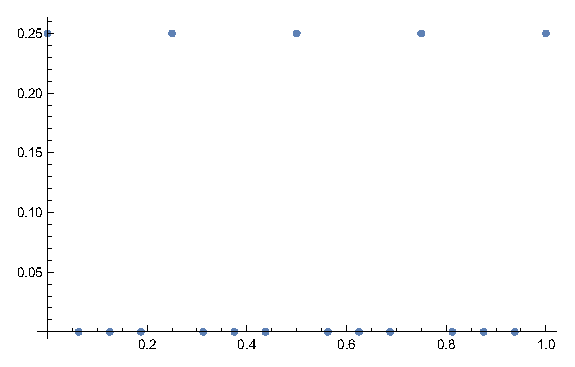
\includegraphics{img/Shor_gr1.eps}

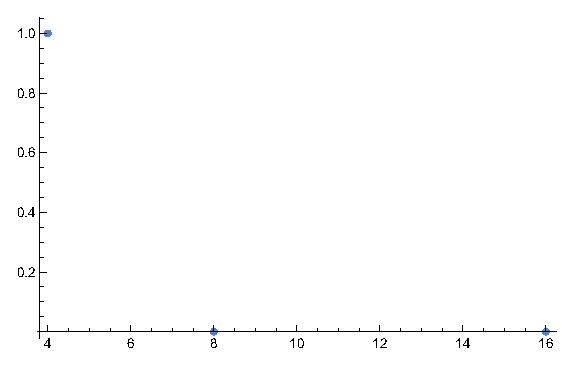
\includegraphics{img/Shor_gr2.eps}

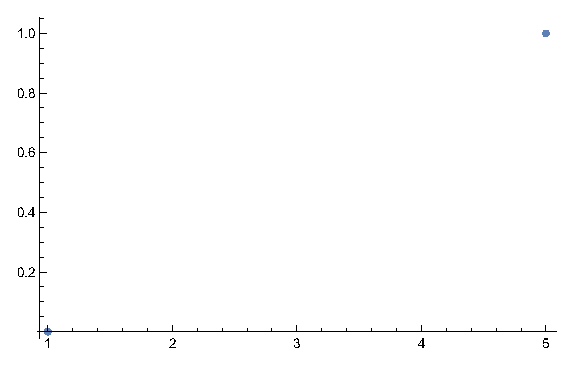
\includegraphics{img/Shor_gr3.eps}

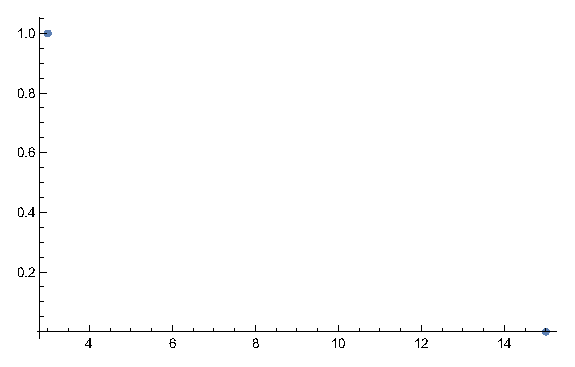
\includegraphics{img/Shor_gr4.eps}

\section{Simulación en Python}

\begin{figure}[H]
\centering 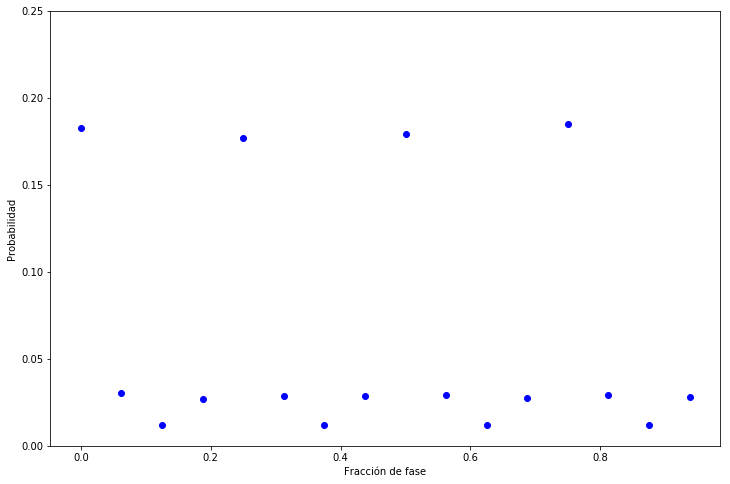
\includegraphics[width=0.9\linewidth]{img/shorlossless.png}
\caption{}
\end{figure}

[0.18265120316248348,
 0.030148605498127055,
 0.0117556126084082,
 0.027068348030583445,
 0.17700021614033762,
 0.028491802773181096,
 0.011881438650927171,
 0.028510782606300467,
 0.17917422966710292,
 0.029450553218688075,
 0.012081135256705483,
 0.027710388875941253,
 0.18489803932544116,
 0.02936951642045106,
 0.012035158723792341,
 0.027772969041529337]


\chapter{Google PageRank}
% El PageRank, nombrado en honor a Larry Page, es una de las medidas de centralidad de los nodos de un grafo más conocidas. Ésta es utilizada para ordenar los sitios web en los resultados de búsqueda de Google, de acuerdo a su importancia.

El algoritmo de PageRank fue desarrollado en 1996 en la Universidad de Stanford por Larry Page y Sergey Brin, los cuales fueron los fundadores de Google.

Este algoritmo se basa en la idea de que sitios web importantes tienen muchos vínculos que apuntan hacia ellos, lo que conduce a pensar en la web como una red ponderada orientada.

Existen muchos otros algoritmos, algunos más eficientes, pero la importancia de PageRank se sustenta en el poder económico de Google.

Ilustraremos el algoritmo de PageRank con un ejemplo sencillo:

Ejemplo:

Consideremos 5 páginas web distintas a las que denotaremos por 1, 2, 3, 4, y 5, y cuyo grafo es:
\vspace{3cm}

Pasos:
\begin{enumerate}
\item Determinar la matriz de adyacencia. Algunos autores denotan la matriz de de adyacencia por M en el protocolo de PageRank

\[
M = \begin{pmatrix}
0 & 0 & 1 & 1 & 1 \\
0 & 0 & 0 & 0 & 1 \\
1 & 0 & 0 & 1 & 1 \\
1 & 0 & 1 & 0 & 0 \\
1 & 1 & 0 & 0 & 0
\end{pmatrix}
\]

\item Sumamos los elementos de cada una de las columnas.

\[
\begin{matrix}
3 & 1 & 2 & 2 & 3
\end{matrix}
\]

Estas sumas representan el número de links que salen del nodo o vértice de la página $p_j$, es decir: 

$I(p_j) \equiv \text{Importancia de la página j}$

$\mathrm{outdeg}(p_j) \equiv \text{número de links que salen de la página } p_j$

$I(p_i) \equiv \sum\limits_{j \in B_i} \frac{I(p_j}{\mathrm{outdeg}(p_j)}$

$B_i \equiv \text{conjunto de páginas qeu son linkeadas}$

\item Dividimos cada elemento de M por la suma de los elementos de la columna a la cual corresponde y llamaremos a la nueva matriz obtenida $M^\prime$

\[
M^\prime = \begin{pmatrix}
0 & 0 & 1/2 & 1/2 & 1/3 \\
0 & 0 & 0 & 0 & 1/3 \\
1/3 & 0 & 0 & 1/2 & 1/3 \\
1/3 & 0 & 1/2 & 0 & 0 \\
1/3 & 1 & 0 & 0 & 0
\end{pmatrix}
\]

\item El siguiente paso es encontrar un vector $\vec{v}$ (algunos autores lo llaman $\vec{I}$) que represente el PageRank de cada una de las páginas. Como tenemos 5 páginas web le asignamos a $\vec{v}$ como valores $\vec{v} = (a,b,c,d,e)^T$, obteniendo así un vector de dimensión $d=5$.

\item Obtenemos los valores de $\{v_i\}$ a partir de los autovalores de $M^\prime$, tal que:

\[
M^\prime \vec{v} = \lambda \vec{v} \text{ con }\lambda \in R
\]

\item Determinamos los autovalores de $M^\prime$

\[
\lambda_1 = 1; \quad \lambda_2 = \frac{-2}{3}; \quad \lambda_3 = \frac{-1}{2}; \quad \lambda_4 = \frac{-1}{3}; \quad \lambda_5 = \frac{1}{3}
\]

Tomaremos sólo $\lambda = 1$ $\rightarrow M^\prime \vec{v} = \vec{v}$ (Ecuación autoconsistente)

\item Hallamos el autovector asociado a $\lambda = 1$. Obteniendo:

\[
a = 6; \quad b = 1; \quad c = \frac{16}{3}; \quad d = \frac{14}{3}; \quad e = 3
\]

\item Finalmente, Google ordena de mayor a menor las componentes de $\vec{v}$, quedándonos:

\[
\begin{matrix}
& & - & a \\
& & - & c \\
\text{Pantalla} & \rightarrow & - & d \\
& & - & e \\
& & - & b
\end{matrix}
\]
\end{enumerate}

La idea de PageRank de Google es que la importancia de una página viene dada por la cantidad de páginas que se enlazan con ella.

Surgen varios problemas:

\begin{enumerate}
  \item Las matrices hyperlink (hiperenlace) pueden tener billones de entradas en filas y columnas.
  \item Calcular los autovectores es un absurdo computacional.
  \item Los estudios muestran que un nodo (página web) tiene un promedio de 10 enlaces, y las demás entradas de la matriz son cero.
  \item No se encuentra $\lambda = 1$ en la mayoría de los casos.
\end{enumerate}

Por esta razón, un remedio (Patching) del algoritmo de PageRank fue el método de las potencias, en el cual la matriz hiperenlace

\[
H_{ij} \equiv \begin{cases}
\frac{1}{\mathrm{outdeg}(P_j)} & \text{si } P_j \in B_i \\
0 & \text{en otro caso}
\end{cases}
\]

debería converger a una solución autoconsistente

\[
I^{k+1} = H I^k
\]

donde se toma un vector $I^{0}$ y se hace interactuar unas 100 veces y el orden mostrado de las páginas es el de $I^{100}$, ordenadas de mayor a menor. Si se normalizan las columnas de la matriz hipervínculo (hiperenlace) $H$, obtenemos otra matriz hiperenlace normalizada E.

\textbf{La matriz E:} se sabe de la teoría de matrices estocásticas que 1 es uno de sus autovalores. Además, también se sabe que la convergencia de $I^k = E I^{k-1}$ a $I = E I$ depende del segundo autovalor de $\lambda_2$ de E y es un hecho que $I^k = E I^{k-1}$ converge rápidamente si $\abs{\lambda_2}$ es
cercano a cero.

\section{El algoritmo de remiendo (parcheo) general}

Asumamos que el caminante recorre el grafo siguiendo la web con una matriz estocástica E con probabilidad $\alpha$, y con probabilidad $1-\alpha$ podrá ir a cualquier página al azar que sea de su interés. La matriz web de este proceso será:

\[
G \equiv \alpha E + \frac{1-\alpha}{N} \mathds{I} \text{Matriz de Google}
\]

$\mathds{I}$ es una matriz en la cual todas las entradas están establecidas en 1, y N el número de nodos.

Propiedades de G:
\begin{enumerate}
\item Es estocástica
\item Irreducible
\item Primitiva
\item El resultado de determinar el estado auto-consistente no depende del vector Google inicial $I^0$
\end{enumerate}

\begin{figure}[H]
\begin{center}
\begin{tabular}{c c c}
 \begin{tikzpicture}[->,>=stealth',shorten >=1pt,thick]
\tikzset{VertexStyle/.style = {draw,circle,thick,
                               minimum size=0.5cm,
                               font=\bfseries},thick} 
\Vertex[a = 90, d = 2.75]{1}  \Vertex[a = 162, d = 2.75]{2}
\Vertex[a = 234, d = 2.75]{3} \Vertex[a = 306, d = 2.75]{4}
\Vertex[a = 18, d = 2.75]{5}
\Edge[label=$1$](2)(1)
\Edge[label=$1$](1)(5)
\Edge[label=$\frac{1}{2}$](3)(1)
\Edge[label=$\frac{1}{2}$](3)(4)
\Edge[label=$1$](4)(5)
\tikzset{EdgeStyle/.style = {->, bend left}}
\Edge[label=$1$](1)(3)
\end{tikzpicture} 
& \begin{tikzpicture}[->,>=stealth',shorten >=1pt,thick]
\tikzset{VertexStyle/.style = {draw,circle,thick,
                               minimum size=0.5cm,
                               font=\bfseries},thick} 
\Vertex[a = 90, d = 2.75]{1}  \Vertex[a = 162, d = 2.75]{2}
\Vertex[a = 234, d = 2.75]{3} \Vertex[a = 306, d = 2.75]{4}
\Vertex[a = 18, d = 2.75]{5}
\Edge[label=$\frac{1}{10}$](5)(4)
\Edge[label=$\frac{1}{10}$](4)(3)
\Edge[label=$\frac{1}{10}$](3)(2)
\Edge[label=$\frac{3}{5}$](2)(1)
\Edge[label=$\frac{3}{5}$](1)(5)
\Edge[label=$\frac{1}{10}$](1)(4)
\Edge[label=$\frac{1}{10}$](4)(2)
\Edge[label=$\frac{1}{10}$](2)(5)
\Edge[label=$\frac{1}{10}$](5)(3)
\Edge[label=$\frac{7}{20}$](3)(1)
\Loop[dist=1cm,dir=NO,label=$\frac{1}{10}$,labelstyle=above](1)  
\Loop[dist=1cm,dir=NOWE,label=$\frac{1}{10}$,labelstyle=above left](2)  
\Loop[dist=1cm,dir=SOWE,label=$\frac{1}{10}$,labelstyle=below left](3)  
\Loop[dist=1cm,dir=SOEA,label=$\frac{1}{10}$,labelstyle=below right](4)  
\Loop[dist=1cm,dir=NOEA,label=$\frac{1}{10}$,labelstyle=above right](5)  
\tikzset{EdgeStyle/.style = {->, bend right}}
\Edge[label=$\frac{1}{10}$,labelstyle=above left](1)(2)
\Edge[label=$\frac{1}{10}$,labelstyle=below left](2)(3)
\Edge[label=$\frac{7}{20}$,labelstyle=below](3)(4)
\Edge[label=$\frac{3}{5}$,labelstyle=below right](4)(5)
\Edge[label=$\frac{1}{10}$,labelstyle=above right](5)(1)
\Edge[label=$\frac{3}{5}$](1)(3)
\Edge[label=$\frac{1}{10}$](3)(5)
\Edge[label=$\frac{1}{10}$](5)(2)
\Edge[label=$\frac{1}{10}$](2)(4)
\Edge[label=$\frac{1}{10}$](4)(1)
\end{tikzpicture} 
 \\
(a) & (b)
\end{tabular}
\caption[Transformación de un grafo al crear la matriz de Google con $\alpha = \frac{1}{2}$]{Transformación de un grafo al crear la matriz de Google con $\alpha = \frac{1}{2}$: Grafo correspondiente a la matriz de adyacencia (a) de la red E (b) remendada de Google G con $\alpha=\frac{1}{2}$}
\end{center}
\end{figure}

\section{Interpretación como una caminata aleatoria}

La asiganación de valores de importancia se puede replantear como la probabilidad de encontrar un caminante aleatorio en cierto nodo del grafo.

\begin{minipage}{0.5\linewidth}
Del proceso:
\begin{align*}
& Pr(x^{(n+1)}=p_i) \\
& =\sum\limits_j G_{i j} Pr(x^{(n)}=p_j)
\end{align*}
\end{minipage}
\begin{minipage}{0.5\linewidth}
De la ley de probabilidad total:
\begin{align*}
& Pr(x^{(n+1)}=p_i) \\
& =\sum\limits_j Pr(x^{(n+1)}=p_i|x^{(n)}=p_j) Pr(x^{(n)}=p_j)
\end{align*}
\end{minipage}
\[
\implies G_{i j} = Pr(x^{(n+1)}=p_i | x^{(n)}=p_j)
\]

En el contexto del Internet, $G_{i j}$ es la probabilidad de que cierto internauta, que se encuentra en la página $p_i$, entre en la página $p_j$. El factor $\alpha E_{i j}$ es la probabilidad de que lo haga presionando un enlace presente en $p_i$, mientras que $\frac{1-\alpha}{N} \mathds{I}$ es la probabilidad de que lo haga introduciendo la URL directamente.

El factor de amortiguamiento es libre y debe ser calibrado. Se suela usar $\alpha = 0.85$

\section{Cuantizando las caminatas aleatorias}

La forma obvia y directa de cuantizar una caminata aleatoria sería sustituir el conjunto de nodos $\{p_i\}$ por el conjunto de kets $\{\ket{i}\}$. Sin embargo, esto lleva a sistemas con operadores no unitarios y no es realizable.

% INSERTAR EJEMPLO AQUÍ
\begin{figure}[H]
\begin{tabular}{c c}
\begin{tikzpicture}[,>=stealth',shorten >=1pt,thick]
\tikzset{VertexStyle/.style = {draw,circle,thick,
                               minimum size=1cm,
                               font=\bfseries},thick} 
\Vertex[x = -2.2, y = 0]{-2}  \Vertex[x = -1.1, y = 0]{-1}
\Vertex[x = 0, y = 0]{0} \Vertex[x = 1.1, y = 0]{1}
\Vertex[x = 2.2, y = 0]{2}
\Edges(-2,-1,0,1,2)
\end{tikzpicture} &
\begin{tikzpicture}[,>=stealth',shorten >=1pt,thick]
\tikzset{VertexStyle/.style = {draw,circle,thick,
                               minimum size=1cm,
                               font=\scriptsize\bfseries},thick} 
\Vertex[x = -2.2, y = 0, L = $\ket{-2}$]{-2}  \Vertex[x = -1.1, y = 0, L = $\ket{-1}$]{-1}
\Vertex[x = 0, y = 0, L = $\ket{0}$]{0} \Vertex[x = 1.1, y = 0, L = $\ket{1}$]{1}
\Vertex[x = 2.2, y = 0, L = $\ket{2}$]{2}
\Edges(-2,-1,0,1,2)
\end{tikzpicture}
\end{tabular}
\end{figure}

Esto nos obliga a buscar maneras alternativas de cuantizar las caminatas aleatorias. La cadena anterior se podría cuantizar agregando un espacio "moneda" al espacio de Hilbert generado por $\{\ket{i}\}$. En este caso, el operador de difusión se interpreta como "lanzar la moneda" para decidir en qué dirección ir.

\begin{align*}
U = \sqrt{p} \ketbra{i+1}{i} \otimes \ketbra{c}{c} + \sqrt{1-p}
\ketbra{i-p}{i} \otimes \ketbra{s}{s} \\
U^\dagger = \sqrt{p} \ketbra{i}{i+1} \otimes \ketbra{c}{c} + \sqrt{1-p}
\ketbra{i}{i-p} \otimes \ketbra{s}{s} \\
U U^\dagger = p \ketbra{i+1}{i+1} \otimes \ketbra{c}{c} + (1-p) \ketbra{i-1}{i-1} \otimes \ketbra{s}{s}
\end{align*}

Al realizar la suma sobre $i$ se tiene $\mathds{1}$, como se deseaba. Sin embargo, esta solución toavía no es satisfactoria, pues exige que $p_{i j}=\frac{1}{outdeg(j)}$ para que $U U^\dagger=\mathds{1}$.

Casi todas las cuantizaciones cometen estos dos pecados, aumentar la dimensión del espacio de Hilbert e imponer condiciones sobre el grafo; y en general, se debe cometer al menos uno de los dos. También existen caminatas cuánticas continuas, no sólo discretas, pero ellas siguen un esquema distinto de la computación cuántica, donde no se busca que el operador de evolución del sistema corresponda a compuertas cuánticas con las cuales construir el operador de difusión, sino directamente al operador de difusión de la caminata cuántica.

\section{Caminata cuántica de Szegedy}

Existe un tipo particular de caminatas aleatorias conocido como caminatas bipartitas. En éstas se tiene dos conjuntos de nodos y sólo ocurren transiciones entre los dos conjuntos, no dentro del mismo.

% INSERTAR EJEMPLO AQUÍ

Szegedy desarrolló una cuantización de estas caminatas. Para esto utilizó operadores de reflexión ($W = \mathds{1} - 2 \ketbra{w}{w}$, similares a los utilizados en el algoritmo de Grover). Aprovechándose del hecho de que un par de reflexiones equivale a una rotación (como en el algoritmo de Grover), creó el siguiente operador de evolución de la caminata: $U = (\mathds{1} - 2 B)(\mathds{1} - 2 A)$, donde A es el proyector sobre las transiciones de la primera partición a la segunda y B de la segunda a la primera.

\begin{minipage}{0.5\linewidth}
\begin{align*}
\ket{\psi_i} &= \ket{i}_1 \otimes \sum\limits_j \sqrt{p_{j i}} \ket{j}_2 \\
A &= \sum\limits_i \ketbra{\psi_i}{\psi_i}
\end{align*}
\end{minipage}
\begin{minipage}{0.5\linewidth}
\begin{align*}
\ket{\psi_i} &= \sum\limits_i \sqrt{p_{i j}} \ket{i}_1 \otimes \ket{i}_2 \\
B &= \sum\limits_j \ketbra{\phi_j}{\phi_j}
\end{align*}
\end{minipage}

Si tomamos un grafo cualquiera y lo duplicamos en la forma de un grafo bipartito con ambas particiones iguales y transiciones iguales en ambos sentidos, podemos cuantizar cualquier tipo de caminata. Sólo hay que pagar el precio de duplicar el espacio de Hilbert generado por $\{\ket{i}\}$: $\mathcal{H}^\prime = \mathcal{H} \otimes \mathcal{H}$.

% INSERTAR EJEMPLO AQUÍ
\begin{figure}[h]
\begin{tabular}{c c c}
\begin{tikzpicture}[->,>=stealth',shorten >=1pt,thick]
\SetGraphUnit{2} 
\tikzset{VertexStyle/.style = {draw,circle,thick,
                               minimum size=0.5cm,
                               font=\Large\bfseries},thick} 
\Vertex{1} \SOWE(1){2} \SOEA(2){3} \SOEA(1){4} 
\Edges(1,2,3) \Edge(1)(4)

\tikzset{EdgeStyle/.style = {->, bend left}}
\Edge(3)(2)
% it's possible with \Edge but Tikz's syntax is allowed too.
\end{tikzpicture} 
&
\begin{tikzpicture}[->,>=stealth',shorten >=1pt,thick]
\tikzset{VertexStyle/.style = {draw,circle,thick,
                               minimum size=0.5cm,
                               font=\bfseries},thick} 
\Vertex[x = 0, y = 0]{1a} \Vertex[x = 0, y = -1]{2a}
\Vertex[x = 0, y = -2]{3a}\Vertex[x = 0, y = -3]{4a}
\Vertex[x = 3, y = 0]{1b} \Vertex[x = 3, y = -1]{2b}
\Vertex[x = 3, y = -2]{3b}\Vertex[x = 3, y = -3]{4b}
\Edge(1a)(2b)	\Edge(1a)(3b)	\Edge(2a)(4b)
\Edge(4a)(2b)
\end{tikzpicture}
&
\begin{tikzpicture}[->,>=stealth',shorten >=1pt,thick]
\tikzset{VertexStyle/.style = {draw,circle,thick,
                               minimum size=0.5cm,
                               font=\bfseries},thick} 
\Vertex[x = 0, y = 0]{1a} \Vertex[x = 0, y = -1]{2a}
\Vertex[x = 0, y = -2]{3a}\Vertex[x = 0, y = -3]{4a}
\Vertex[x = 3, y = 0]{1b} \Vertex[x = 3, y = -1]{2b}
\Vertex[x = 3, y = -2]{3b}\Vertex[x = 3, y = -3]{4b}
\Edge(2b)(1a)	\Edge(3b)(1a)	\Edge(4b)(2a)
\Edge(4b)(1a)
\end{tikzpicture}
\end{tabular}
\end{figure}

En estos casos, podemso escribir el operador de difusión en términos de sólo A, pues como la segunda partición es un reflejo de la primera, $B = A^T$. Entonces: $U = (2 A^T - \mathds{1})(2 A - \mathds{1})$

\[
\implies = (2 S A S - \mathds{1})(2 A - \mathds{1}) = S (2 A - \mathds{1}) S (2
A - \mathds{1}) = [S (2 A - \mathds{1})]^2
\]

Donde $S$ es el operador SWAP, $S = \sum\limits_{i j} \ketbra{j i}{i j}$

Tomando $W = (2 A - \mathds{1})$, el operador de difusión es

\begin{equation}
    U = (S W)^2
\end{equation}

\section{PageRank cuántico}

Finalmente, procedemos a cuántizar el algoritmo de PageRank. Partimos del hecho de que el algoritmo de PageRank se puede formular como una caminata algeatoria, cuya matriz de probabilidades es la matriz de Google, G. Entonces seguimos el procedimiento de Szegedy, sustituyendo $p_{i j}$ por $G_{i j}$.

Ahora, definimos el valor de PageRank cuántico en el paso $m$ como:

\begin{align*}
I_q(P_i,m) &= \ket{U^{\dagger m}(\mathds{1} \otimes \ketbra{i}{i})} \\
\ket{\psi_0} &= \frac{1}{\sqrt{N}} \sum\limits_i \ket{\psi_i}
\end{align*}

Esto equivale a realizar $m$ pasos de la caminata con $\ket{\psi_0}$ como estado inicial y realizar una medida proyeciva sobre $\ket{i}_2$.

Nota: $I_q$ no converge, sino que oscila, así que se toma el centro de las oscilacioens como la medida de importancia de las páginas. Esto se hace promediando $I_q$ sobre $m$: $\langle I_q(P_i) \rangle = \frac{1}{M} \sum\limits_{m=0}^{M-1} I_q(P_i,m)$ 

\section{Circuitos de las caminatas cuánticas de Szegedy}

Loke y Wang \cite{loke} proponen un esquema para construir eficientemente algoritmos de las caminatas cuánticas de Szegedy. Este esquema consiste en separar las reflexiones del algoritmo en distintas etapas y realizar reflexiones alrededor de estados de la base computacional.

Sea el operador de reflexión del operador de difusión

\begin{equation}
    W = 2 \sum\limits_i \ketbra{\psi_i}{\psi_i} - \mathds{1} = 2 \sum\limits_i \ketbra{i}{i} \otimes \ketbra{\psi_i^\prime}{\psi_i^\prime} - \mathds{1}
\end{equation}

Donde $\ket{\psi_i^\prime} = \sum\limits_j \sqrt{p_{j i}} \ket{j}_2$

Si le aplicamos la transformación unitaria $K = \sum\limits_i \ketbra{i}{i} \otimes K_i$ tal que $U_i \ket{\psi_i^\prime} = \ket{b}$, donde  $\ket{b}$ es un estado de la base computacional, tendremos:

\begin{multline}
K W K^\dagger = K (2 A - \mathds{1}) K^\dagger = 2 K A K^\dagger - \mathds{1} = 2 \sum\limits_i \ketbra{i}{i} \otimes K_i \ketbra{\psi_i^\prime}{\psi_i^\prime} K_i^\dagger) - \mathds{1} \\ = 2 \sum\limits_i \ketbra{i}{i} \otimes \ketbra{b}{b}) - \mathds{1} = 2 \mathds{1}_1 \otimes \ketbra{b}{b}_2 - \mathds{1} = D
\end{multline}

Lo cual se puede implementar fácilmente con compuertas de fase controladas, ya que es una reflexión alrededor de un estado de la base computacional del segundo registro. Sin embargo, esto todavía requeriría hallar $N$ $K_i$ distintos para un grafo de $N$ nodos. Para disminuir la cantidad de $K_i$ a hallar, se pueden aprovechar simetrías en la matriz de adyacencia del grafo. Si separamos el grafo en subgrafos cíclicos, bastaría con hallar un $K_i$ por subgrafo. En los grafos cíclicos, cada fila de la matriz de adyacencia, y de la matriz de Google, es una permutación de la anterior. Lo mismo sucede con los estados asociados a cada uno de los nodos, así que, con un operador de permutación $T$, se podrían convertir los estados de todos los nodos de un grafo cíclico en un mismo estado de referencia. Por ejemplo, supongamos un grafo, cuyos estados $\ket{\psi_i^\prime}$ son:

\begin{equation}
    \begin{array}{cc}
        \ket{\psi_0^\prime} = 
        \begin{pmatrix}
            \sqrt{0.0375} \\ \sqrt{0.8875} \\ \sqrt{0.8875} \\ \sqrt{0.8875}
        \end{pmatrix} &
        \ket{\psi_1^\prime} = 
        \begin{pmatrix}
            \sqrt{0.8875} \\ \sqrt{0.0375} \\ \sqrt{0.8875} \\ \sqrt{0.8875}
        \end{pmatrix} \\
        \ket{\psi_2^\prime} = 
        \begin{pmatrix}
            \sqrt{0.8875} \\ \sqrt{0.8875} \\ \sqrt{0.0375} \\ \sqrt{0.8875}
        \end{pmatrix} &
        \ket{\psi_3^\prime} = 
        \begin{pmatrix}
            \sqrt{0.8875} \\ \sqrt{0.8875} \\ \sqrt{0.8875} \\ \sqrt{0.0375}
        \end{pmatrix}
    \end{array}
\end{equation}

Entonces, el operador de permutación

\begin{equation}
    T = X(1) \text{CNOT}(1, 0)
\end{equation}

Permite transformar $\ket{\psi_1^\prime},\ket{\psi_2^\prime},\ket{\psi_3^\prime}$ en $\ket{\psi_0^\prime}$ de la siguiente manera:

\begin{equation}
    \begin{array}{cc}
        \ket{\psi_0^\prime} = T^\dagger \ket{\psi_1^\prime} = T^3 \ket{\psi_1^\prime} = T^2 \ket{\psi_2^\prime} = T \ket{\psi_3^\prime}
    \end{array}
\end{equation}

\begin{figure}[H]
\[\Qcircuit @C=1.4em @R=1.8em {
        & \targ     & \qw      & \qw \\
        & \ctrl{-1} & \gate{X} & \qw \\
} 
\]
\caption[Operador de permutación]{Operador de permutación $T$}
\label{fig:T}
\end{figure}

Luego, siguiendo esta idea, $K_i = K_b^\dagger T_i$, donde $K_b^\dagger \ket{\psi_r^\prime} = \ket{b}$ y $T_i \ket{\psi_i^\prime} = \ket{\psi_r^\prime}$. En otras palabras, $\{K_b\}$ representa el conjunto de $K_i$ necesarios después de separar el grafo, uno por cada subgrafo cíclico; $\ket{\psi_r^\prime}$ es un estado de referencia de cada subgrafo cíclico y podría ser el estado asociado a alguno de los nodos de ese subgrafo; $T_i$ es un operador que transforma el estado de cada nodo en el estado de referencia del subgrafo cíclico correspondiente. En caso de haber elegido $\ket{\psi_r^\prime}$ como el estado de alguno de los nodos del subgrafo cíclico, entonces $T_i$ puede ser un mismo operador de permutción aplicado repetidas veces para todos los nodos del mismo subgrafo, como en el ejemplo anterior.

\begin{figure}[H]
\[\Qcircuit @C=1.4em @R=1.8em {
        \lstick{\text{Registro 1}}& {/}\qw & \ctrl{1}   & \ctrl{1}           & \qw      & \ctrl{1}   & \ctrl{1}           & \qswap     & \qw \\
        \lstick{\text{Registro 2}}& {/}\qw & \gate{T_i} & \gate{K_b^\dagger} & \gate{D} & \gate{K_b} & \gate{T_i^\dagger} & \qswap\qwx & \qw \\
& & & & \rstick{\hspace{-13pt} 2 \text{ veces}}
\gategroup{2}{3}{2}{8}{1.5em}{_\}}
} 
\]
\caption[Circuito de Loke para las caminatas cuánticas de Szegedy]{Circuito de Loke para las caminatas cuánticas de Szegedy}
\label{fig:lokecircuit}
\end{figure}

En resumen, el proceso para construir el circuito de una caminata de Szegedy es:

\begin{enumerate}
    \item Hallar la matriz de Google del grafo.
    \item Separar las filas de la matriz en grupos de filas tales que las filas de cada grupo sean permutaciones una de la otra.
    \item Hallar los operadores de permutación $T_i$.
    \item Hallar los operadores $K_b$ que conviertan un estado de referencia $\ket{\phi_{r_i}}$ de cada grupo en un mismo estado de referencia $\ket{b}$ de la base computacional.
    \item Hallar el operador de reflexión D.
    \item Construir el operador de difusión a partir del circuito de la figura \ref{fig:lokecircuit}.
\end{enumerate}

Loke y Wang sólo muestran como realizar $K_i$ para unos pocos casos particulares de caminatas cuánticas de Szegedy que utilizan como ejemplo en su paper. En estre trabajo mostramos cómo realizar cualquier $K_i$ para caminatas cuánticas de Szegedy asociadas a grafos de cuatro nodos.

Todos los coeficientes de los estados involucrados en el algoritmo de PageRank son reales positivos o cero. Es decir, que los qubits individuales que forman estos estados pertenecen todos al arco de semicircunferencia que va de $+\hat{z}$ a $-\hat{z}$ pasando por $+\hat{x}$. Esto indica que los operadores $K_i$ deben poder construirse a partir de compuertas $Ry(\theta)$ y compuertas $Ry(\theta)$ condicionadas tomando $0 \leq \theta \leq \pi$.

En lo que sigue se considerará $\ket{b} = \ket{0}$ y que los grafos son de cuatro nodos. De esta manera, podemos asumir que

\begin{equation}
    K_i = CRy_n(0,1,\theta_{11}) CRy_b(0,1,\theta_{10}) Ry(0,\theta_{00})
\end{equation}

\begin{figure}[H]
\[\Qcircuit @C=1.4em @R=1.8em {
& \gate{Ry(\theta_{00})} & \ctrlo{1}               & \ctrl{1}               & \qw \\
& \qw                    & \gate{Ry(\theta_{10})}  & \gate{Ry(\theta_{11})} & \qw \\
} \]
\caption{Circuito de $K_i$}
\end{figure}

Entonces, para hallar $K_i$, debemos resolver la siguiente ecuación y hallar $\theta_{11}, \theta_{10}, \theta_{00}$

\begin{equation}
    CRy_n(0,1,\theta_{11}) CRy_b(0,1,\theta_{10}) Ry(0,\theta_{00}) \ket{0} = \ket{\phi_{r_i}}
\end{equation}

Sin embargo, esto conduce a un sistema de cuatro ecuaciones y tres variables. Para poder resolver este sistema por métodos numéricos se modifica la ecuación de la siguiente manera, sabiendo que $\theta_x$ debe ser $n 2\pi$, donde $n$ es entero.

\begin{align}
    \cos(\frac{\theta_{00}}{2}) \cos(\frac{\theta_{10}}{2}) &= \sqrt{G_1} \\
    \cos(\frac{\theta_{00}}{2}) \sin(\frac{\theta_{10}}{2}) &= \sqrt{G_2} \\
    \cos(\frac{\theta_{11}}{2}) \sin(\frac{\theta_{00}}{2}) &= \sqrt{G_3} \\
    \sin(\frac{\theta_{00}}{2}) \sin(\frac{\theta_{11}}{2}) &= \sqrt{G_4}
\end{align}

Esto se puede solucionar recordando la normalización de los estados cuánticos y de las matrices estocásticas, entonces, sabemos que $G_4 = 1 - (G_1 + G_2 + G_3)$. Por lo que podemos reducir el sistema de ecuaciones a un de tres variables

\begin{align}
    \cos(\frac{\theta_{00}}{2}) \cos(\frac{\theta_{10}}{2}) &= \sqrt{G_1}
    \label{eq:crot1} \\
    \cos(\frac{\theta_{00}}{2}) \sin(\frac{\theta_{10}}{2}) &= \sqrt{G_2}
    \label{eq:crot2} \\
    \cos(\frac{\theta_{11}}{2}) \sin(\frac{\theta_{00}}{2}) &= \sqrt{G_3}
\end{align}

Sumando \ref{eq:crot1} y \ref{eq:crot2}, y aplicando $\cos^2(\theta) + \sin^2(\theta) = 1$, se tiene:

\begin{align}
    \cos^2(\frac{\theta_{00}}{2}) \cos^2(\frac{\theta_{10}}{2}) &= G_1
    \label{eq:crot3} \\
    \cos^2(\frac{\theta_{00}}{2}) &= G_1 + G_2
    \label{eq:crot4} \\
    \cos^2(\frac{\theta_{11}}{2}) \sin^2(\frac{\theta_{00}}{2}) &= G_3
    \label{eq:crot5}
\end{align}

Ahora, sustituyendo \ref{eq:crot4} en \ref{eq:crot3} y \ref{eq:crot5}, y volviendo a aplicar la misma propiedad trigonométrica, se tiene:

\begin{align}
    \cos^2(\frac{\theta_{10}}{2}) &= \frac{G_1}{G_1 + G_2} \\
    \cos^2(\frac{\theta_{00}}{2}) &= G_1 + G_2 \\
    \cos^2(\frac{\theta_{11}}{2}) &= \frac{G_3}{1-(G_1 + G_2)}
\end{align}

Finalmente, se tiene que los ángulos de las rotaciones deben ser:

\begin{align}
    \theta_{00} &= 2 \cos^{-1}\left(\sqrt{G_1 + G_2}\right) \\
    \theta_{10} &= 2 \cos^{-1}\left(\sqrt{\frac{G_1}{G_1 + G_2}}\right) \\
    \theta_{11} &= 2 \cos^{-1}\left(\sqrt{\frac{G_3}{1 - (G_1 + G_2)}}\right)
\end{align}

\section{Simulaciones}

Se han realizado simulaciones del algoritmo de PageRank con un grafo estrella, un grafo corona, un grafo árbol y un grafo aleatorio, todos de cuatro nodos. Se han realizado simulaciones con y sin pérdidas. El código de las simulaciones se encuentra en el apéndice \ref{ch:pagerankcod}.

\subsection{Grafo estrella}

En la figura \ref{fig:star} se observa el grafo estrella utilizado para esta simulación. Este grafo es simétrico, por lo tanto, su matriz de adyacencia es hermítica% y es un ejemplo de un grafo con el cual no necesitaríamos el esquema de Szegedy para realizar una caminata cuántica
. Este no es el caso, sin embargo, una vez convertimos el grafo en uno ponderado. La matriz estocástica $E$ no es hermítica, y por extensión la matriz de Google tampoco lo es.

\begin{figure}[H]
    \centering
    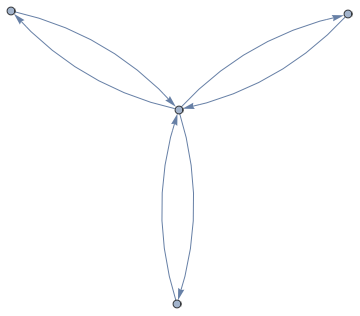
\includegraphics[width=0.5\linewidth]{img/star.png}
    \caption[Grafo estrella]{Grafo estrella}
    \label{fig:star}
\end{figure}

\begin{equation}
    A =
    \begin{pmatrix}
        0 & 1 & 1 & 1 \\
        1 & 0 & 0 & 0 \\
        1 & 0 & 0 & 0 \\
        1 & 0 & 0 & 0
    \end{pmatrix}
\end{equation}

\begin{equation}
    E = 
    \begin{pmatrix}
        0 & 1 & 1 & 1 \\
        \frac{1}{3} & 0 & 0 & 0 \\
        \frac{1}{3} & 0 & 0 & 0 \\
        \frac{1}{3} & 0 & 0 & 0
    \end{pmatrix}
\end{equation}

\begin{equation}
    G =
    \begin{pmatrix}
        \frac{3}{80} & \frac{71}{80} & \frac{71}{80} & \frac{71}{80} \\
        \frac{77}{240} & \frac{3}{80} & \frac{3}{80} & \frac{3}{80} \\
        \frac{77}{240} & \frac{3}{80} & \frac{3}{80} & \frac{3}{80} \\
        \frac{77}{240} & \frac{3}{80} & \frac{3}{80} & \frac{3}{80}
    \end{pmatrix}
\end{equation}

Los tres nodos exteriores de este grafo, además, forman lo que hemos llamado un subgrafo cíclico, por lo que para este grafo necesitaremos dos operadores $K_b$, unos para estos tres nodos y otro para el nodo central. Las figuras \ref{fig:starkb1} - \ref{fig:lokestar} muestran cómo construir el circuito del operador de difusión de la caminata de Szegedy asociada a la matriz de Google de este grafo.

\begin{figure}[H]
\[\Qcircuit @C=1.4em @R=1.8em {
& \gate{Ry(1.85806)} & \ctrlo{1}           & \ctrl{1}          & \qw \\
& \qw                & \gate{Ry(2.48274)}  & \gate{Ry(1.5708)} & \qw \\
} \]
\caption{Circuito de $K_1$ para el grafo estrella}
\label{fig:starkb1}
\end{figure}

\begin{figure}[H]
\[\Qcircuit @C=1.4em @R=1.8em {
& \gate{Ry(0.554811)} & \ctrlo{1}            & \ctrl{1}          & \qw \\
& \qw                 & \gate{Ry(0.405465)}  & \gate{Ry(1.5708)} & \qw \\
} \]
\caption{Circuito de $K_2$ para el grafo estrella}
\label{fig:starkb2}
\end{figure}

\begin{figure}[H]
\[\Qcircuit @C=1.4em @R=1.8em {
& \ctrlo{1}                   & \qw                 & \ctrlo{1}           & \qw \\
& \ctrlo{1}                   & \qw                 & \ctrlo{1}           & \qw \\
& \multigate{1}{K_1^\dagger} & \multigate{1}{K_1} & \multigate{1}{K_2} & \qw \\
& \ghost{K_1^\dagger}        & \ghost{K_1}        & \ghost{K_2}        & \qw \\
} 
\]
\caption[$K_b$ del grafo estrella]{$K_b$ del grafo estrella}
\label{fig:starkb}
\end{figure}

\begin{figure}[H]
\[\Qcircuit @C=1.4em @R=1.8em {
& \gate{Id} & \qw \\
& \gate{Id} & \qw \\
} 
\]
\caption[$T$ del grafo estrella]{$T$ del grafo estrella}
\label{fig:starT}
\end{figure}

\begin{figure}[H]
\[\Qcircuit @C=1.4em @R=1.8em {
& \gate{H} & \multigate{3}{K_b} & \qw \\
& \gate{H} & \ghost{K_b}        & \qw \\
& \qw      & \ghost{K_b}        & \qw \\
& \qw      & \ghost{K_b}        & \qw \\
} 
\]
\caption{Preparación del estado inicial para la caminata en el grafo estrella}
\label{fig:starinit}
\end{figure}

\begin{figure}[H]
\[ \Qcircuit @C=1.4em @R=1.8em {
\lstick{\ket{0}} & {/^4} \qw & \gate{Init} & \gate{K_b^\dagger} & \gate{D} & \gate{K_b} & \gate{SWAP} & \meter & \cw \\
                 & & & & \rstick{2m \text{ veces}}
\gategroup{1}{4}{1}{7}{1.3em}{_\}}
} \]
\caption{Circuito del PageRank cuántico  del grafo estrella}
\label{fig:lokestar}
\end{figure}

En la figura \ref{fig:inststarlossless} se puede observar la gráfica del PageRank cuántico instantáneo sin relajación. En esta figura se puede observar claramente la naturaleza sinusoidal de este algoritmo, por estar basado en reflexiones. Como se puede observar, ambas figuras son bastante similares. La diferencia está en que en el caso de la simulación matemática, el PageRank cuántico de los tres nodos exteriores se solapan perfectamente, mientras que en la simulación circuital, no. Esto se debe a la limitada precisión numérica del solucionador de ecuaciones maestras.

\begin{figure}[H]
    \centering
    \begin{subfigure}[m]{0.45\textwidth}
        \centering
        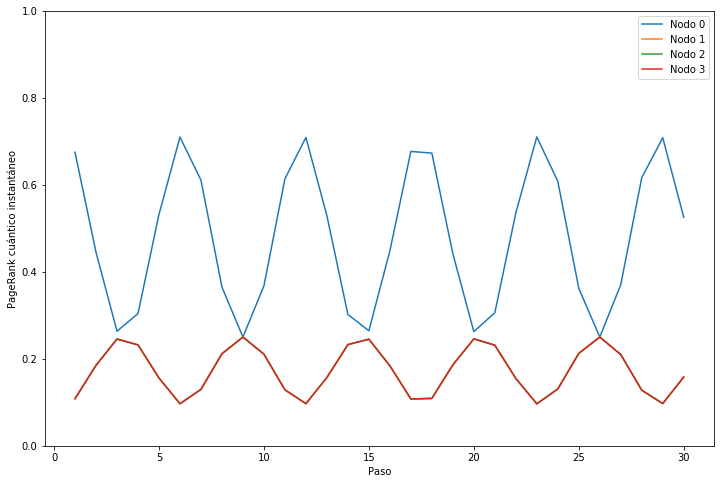
\includegraphics[width=0.9\linewidth]{img/star-inst-M.png}
        \caption{Wolfram Mathematica}
    \end{subfigure}
    \begin{subfigure}[m]{0.45\textwidth}
        \centering
        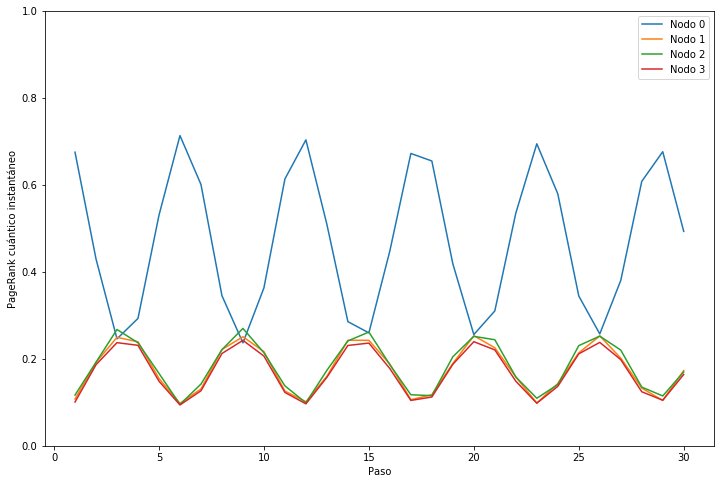
\includegraphics[width=0.9\linewidth]{img/star-inst-lossless.png}
        \caption{Python}
    \end{subfigure}
    \caption[PageRank cuántico instantáneo del grafo estrella sin pérdidas]{PageRank cuántico instantáneo del grafo estrella sin pérdidas}
    \label{fig:inststarlossless}
\end{figure}

En el caso del PageRank promedio, en la figura \ref{fig:meanstarlossless} podemos ver cómo este valor sí converge, a diferencia del PageRank instantaneo, el cuál oscila alrededor del valor de convergencia del PageRank promedio.

\begin{figure}[H]
    \centering
    \begin{subfigure}[m]{0.45\textwidth}
        \centering
        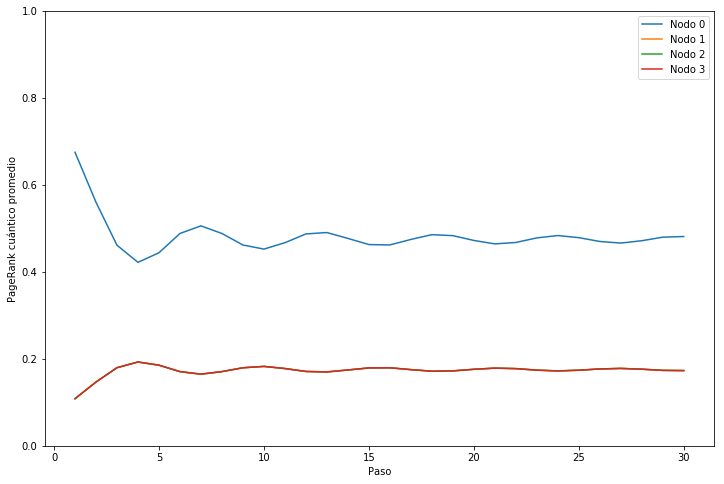
\includegraphics[width=0.9\linewidth]{img/star-mean-M.png}
        \caption{Wolfram Mathematica}
    \end{subfigure}
    \begin{subfigure}[m]{0.45\textwidth}
        \centering
        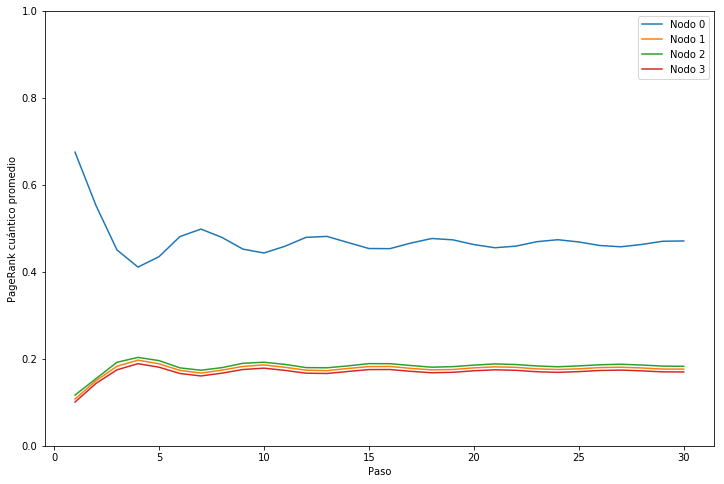
\includegraphics[width=0.9\linewidth]{img/star-mean-lossless.png}
        \caption{Python}
    \end{subfigure}
    \caption[PageRank cuántico promedio del grafo estrella sin pérdidas]{PageRank cuántico promedio del grafo estrella sin pérdidas}
    \label{fig:meanstarlossless}
\end{figure}

Ahora, compararemos los resultados de la simulación circuital con y sin pérdidas. Como se puede ver en la figura (FIGURA), en el caso con pérdidas, <++>

\begin{figure}[H]
    \centering
    \begin{subfigure}[m]{0.45\textwidth}
        \centering
        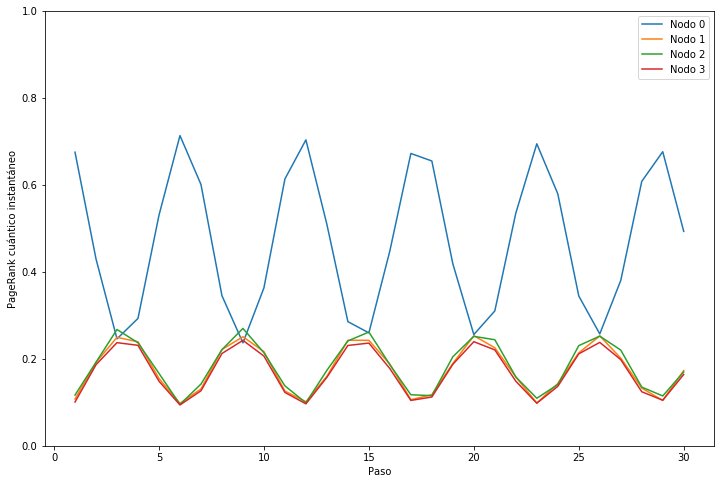
\includegraphics[width=0.9\linewidth]{img/star-inst-lossless.png}
        \caption{Sin relajación}
    \end{subfigure}
    \begin{subfigure}[m]{0.45\textwidth}
        \centering
        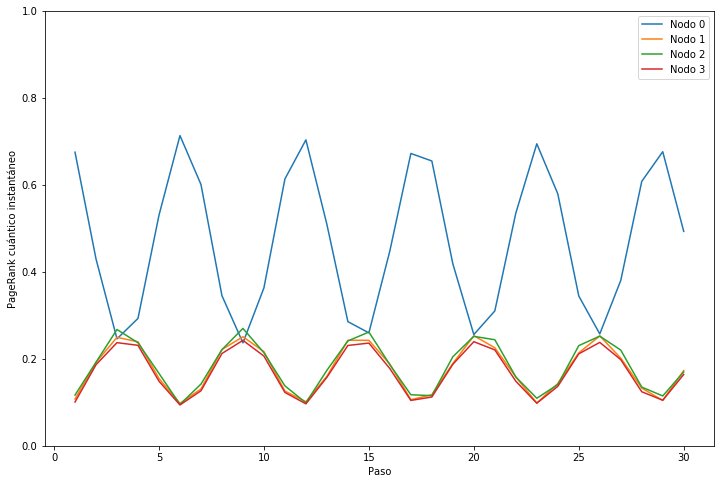
\includegraphics[width=0.9\linewidth]{img/star-inst-lossy.png}
        \caption{Con relajación}
    \end{subfigure}
    \caption[PageRank cuántico instantaneo del grafo estrella con y sin pérdidas]{PageRank cuántico instantaneo del grafo estrella con y sin pérdidas}
    \label{fig:inststarlossy}
\end{figure}

\begin{figure}[H]
    \centering
    \begin{subfigure}[m]{0.45\textwidth}
        \centering
        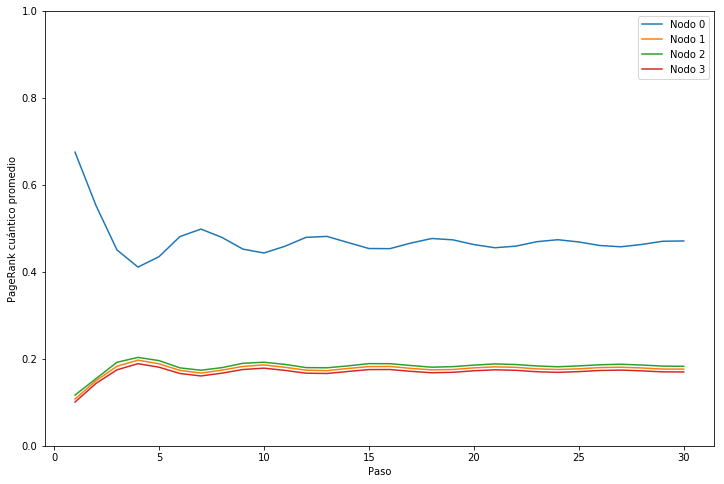
\includegraphics[width=0.9\linewidth]{img/star-mean-lossless.png}
        \caption{Sin relajación}
    \end{subfigure}
    \begin{subfigure}[m]{0.45\textwidth}
        \centering
        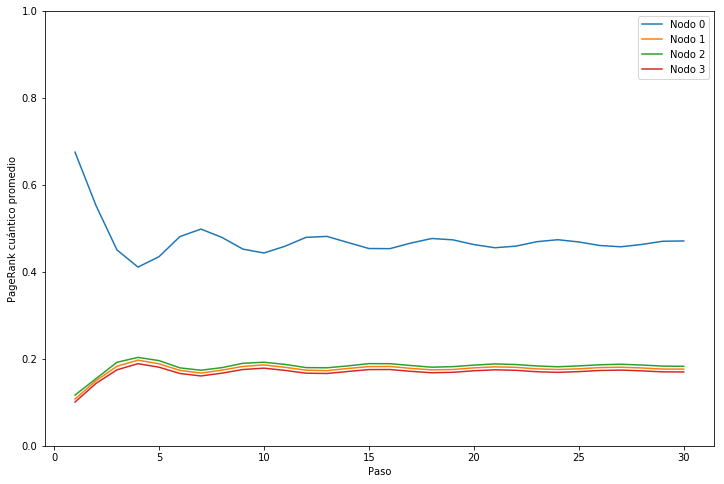
\includegraphics[width=0.9\linewidth]{img/star-mean-lossy.png}
        \caption{Con relajación}
    \end{subfigure}
    \caption[PageRank cuántico promedio del grafo estrella con y sin pérdidas]{PageRank cuántico promedio del grafo estrella con y sin pérdidas}
    \label{fig:meanstarlossy}
\end{figure}

\subsection{Grafo corona}

\begin{equation}
    A =
    \begin{pmatrix}
        0 & 1 & 1 & 0 \\
        1 & 0 & 1 & 0 \\
        1 & 1 & 0 & 0 \\
        1 & 1 & 1 & 0 \\
    \end{pmatrix}
\end{equation}

\begin{equation}
    E =
    \begin{pmatrix}
        0 & \frac{1}{3} & \frac{1}{3} & \frac{1}{4} \\
        \frac{1}{3} & 0 & \frac{1}{3} & \frac{1}{4} \\
        \frac{1}{3} & \frac{1}{3} & 0 & \frac{1}{4} \\
        \frac{1}{3} & \frac{1}{3} & \frac{1}{3} & \frac{1}{4} \\
    \end{pmatrix}
\end{equation}

\begin{equation}
    G =
    \begin{pmatrix}
        \frac{3}{80} & \frac{77}{240} & \frac{77}{240} & \frac{1}{4} \\
        \frac{77}{240} & \frac{3}{80} & \frac{77}{240} & \frac{1}{4} \\
        \frac{77}{240} & \frac{77}{240} & \frac{3}{80} & \frac{1}{4} \\
        \frac{77}{240} & \frac{77}{240} & \frac{77}{240} & \frac{1}{4} \\
    \end{pmatrix}
\end{equation}

\begin{figure}[H]
    \centering
    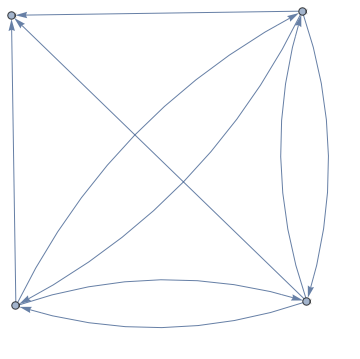
\includegraphics[width=0.5\linewidth]{img/crown.png}
    \caption[Grafo corona]{Grafo corona}
    \label{fig:crown}
\end{figure}

\begin{figure}[H]
    \centering
    \begin{subfigure}[m]{0.45\textwidth}
        \centering
        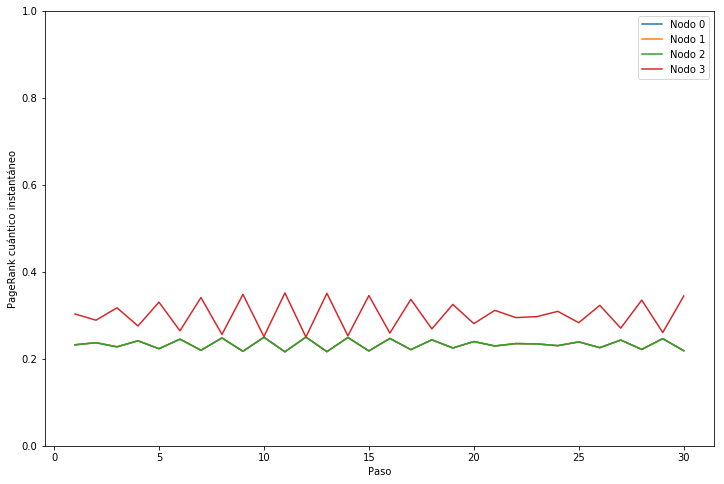
\includegraphics[width=0.9\linewidth]{img/crown-inst-M.png}
        \caption{Wolfram Mathematica}
    \end{subfigure}
    \begin{subfigure}[m]{0.45\textwidth}
        \centering
        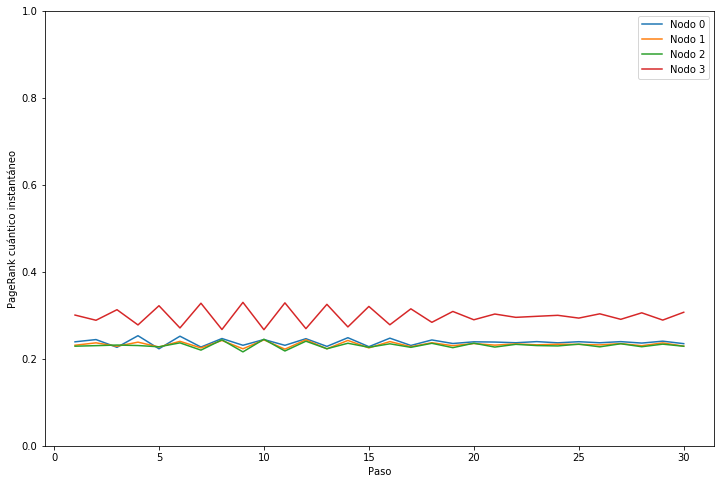
\includegraphics[width=0.9\linewidth]{img/crown-inst-lossless.png}
        \caption{Python}
    \end{subfigure}
    \caption[PageRank cuántico instantáneo del grafo corona sin pérdidas]{PageRank cuántico instantáneo del grafo corona sin pérdidas}
    \label{fig:instcrownlossless}
\end{figure}

\begin{figure}[H]
    \centering
    \begin{subfigure}[m]{0.45\textwidth}
        \centering
        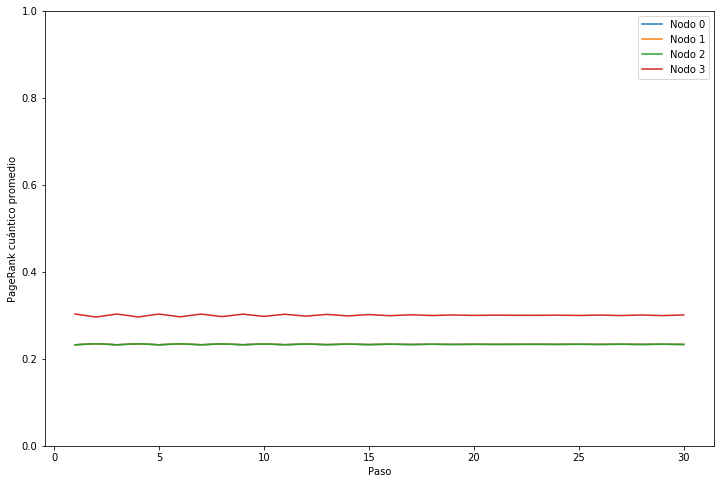
\includegraphics[width=0.9\linewidth]{img/crown-mean-M.png}
        \caption{Wolfram Mathematica}
    \end{subfigure}
    \begin{subfigure}[m]{0.45\textwidth}
        \centering
        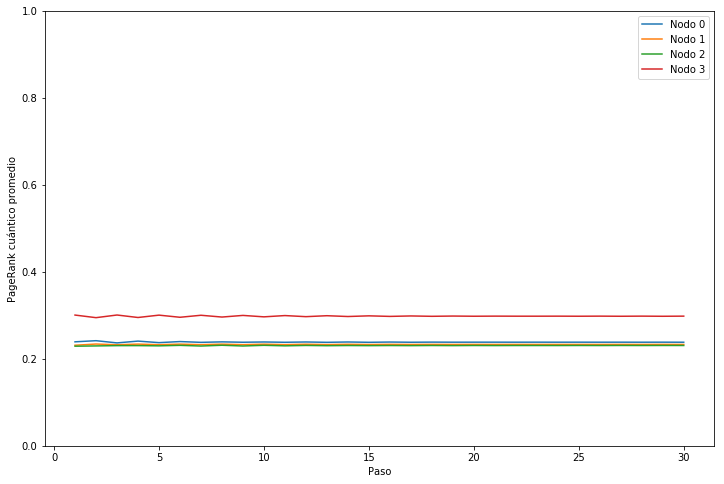
\includegraphics[width=0.9\linewidth]{img/crown-mean-lossless.png}
        \caption{Python}
    \end{subfigure}
    \caption[PageRank cuántico promedio del grafo corona sin pérdidas]{PageRank cuántico promedio del grafo corona sin pérdidas}
    \label{fig:meancrownlossless}
\end{figure}

\subsection{Grafo árbol}

\begin{equation}
    A = 
    \begin{pmatrix}
        0 & 0 & 0 & 0 \\
        1 & 0 & 0 & 0 \\
        1 & 0 & 0 & 0 \\
        0 & 1 & 0 & 0 \\
    \end{pmatrix}
\end{equation}

\begin{equation}
    E =
    \begin{pmatrix}
        0 & 0 & \frac{1}{4} & \frac{1}{4} \\
        \frac{1}{2} & 0 & \frac{1}{4} & \frac{1}{4} \\
        \frac{1}{2} & 0 & \frac{1}{4} & \frac{1}{4} \\
        0 & 1 & \frac{1}{4} & \frac{1}{4} \\
    \end{pmatrix}
\end{equation}

\begin{equation}
    G =
    \begin{pmatrix}
        \frac{3}{80} & \frac{3}{80} & \frac{1}{4} & \frac{1}{4} \\
        \frac{37}{80} & \frac{3}{80} & \frac{1}{4} & \frac{1}{4} \\
        \frac{37}{80} & \frac{3}{80} & \frac{1}{4} & \frac{1}{4} \\
        \frac{3}{80} & \frac{71}{80} & \frac{1}{4} & \frac{1}{4} \\
    \end{pmatrix}
\end{equation}

\begin{figure}[H]
    \centering
    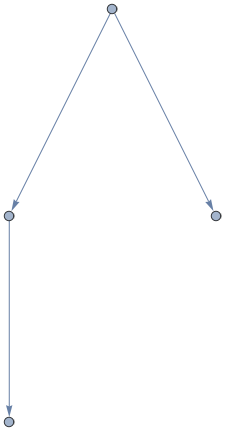
\includegraphics[width=0.5\linewidth]{img/tree.png}
    \caption[Grafo árbol]{Grafo árbol}
    \label{fig:tree}
\end{figure}

\begin{figure}[H]
    \centering
    \begin{subfigure}[m]{0.45\textwidth}
        \centering
        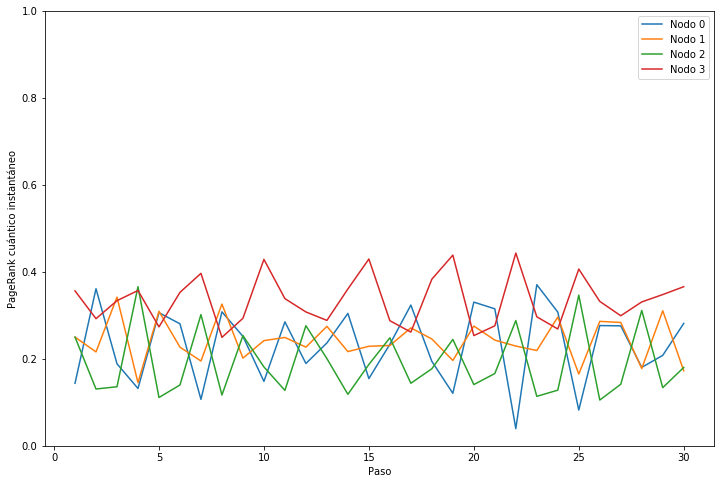
\includegraphics[width=0.9\linewidth]{img/tree-inst-M.png}
        \caption{Wolfram Mathematica}
    \end{subfigure}
    \begin{subfigure}[m]{0.45\textwidth}
        \centering
        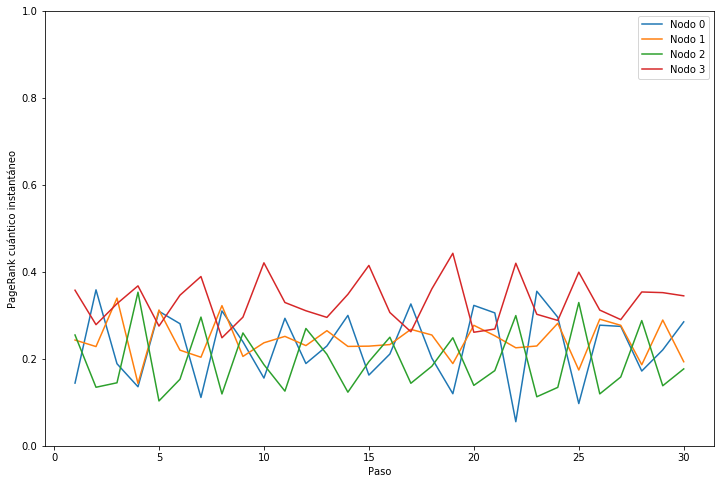
\includegraphics[width=0.9\linewidth]{img/tree-inst-lossless.png}
        \caption{Python}
    \end{subfigure}
    \caption[PageRank cuántico instantáneo del grafo árbol sin pérdidas]{PageRank cuántico instantáneo del grafo árbol sin pérdidas}
    \label{fig:insttreelossless}
\end{figure}

\begin{figure}[H]
    \centering
    \begin{subfigure}[m]{0.45\textwidth}
        \centering
        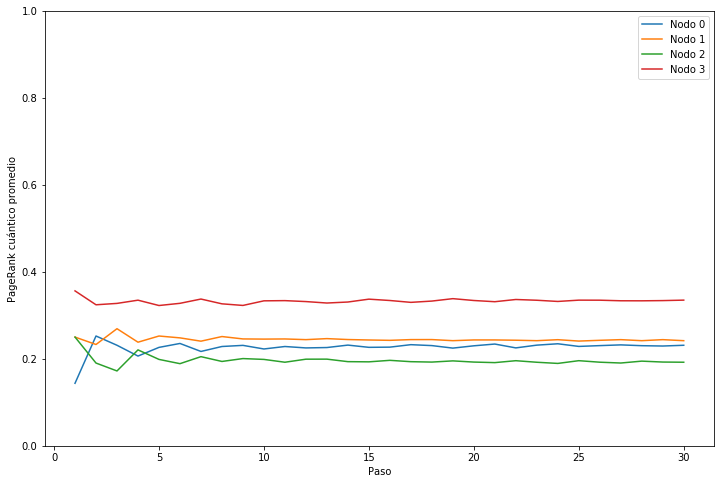
\includegraphics[width=0.9\linewidth]{img/tree-mean-M.png}
        \caption{Wolfram Mathematica}
    \end{subfigure}
    \begin{subfigure}[m]{0.45\textwidth}
        \centering
        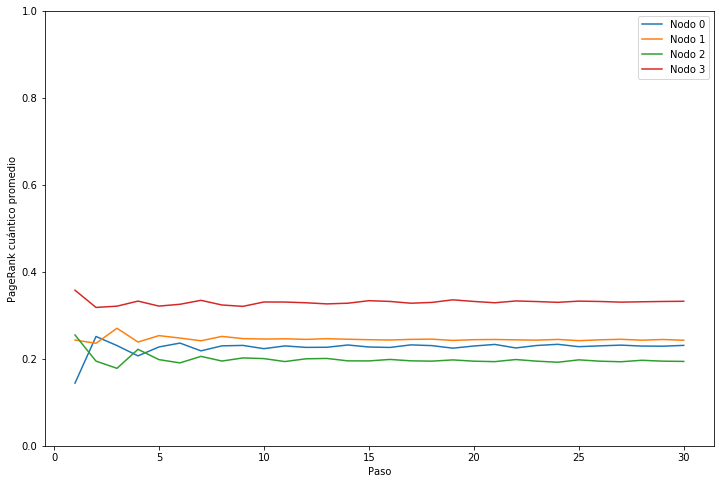
\includegraphics[width=0.9\linewidth]{img/tree-mean-lossless.png}
        \caption{Python}
    \end{subfigure}
    \caption[PageRank cuántico promedio del grafo árbol sin pérdidas]{PageRank cuántico promedio del grafo árbol sin pérdidas}
    \label{fig:meantreelossless}
\end{figure}

\begin{figure}[H]
    \centering
    \begin{subfigure}[m]{0.45\textwidth}
        \centering
        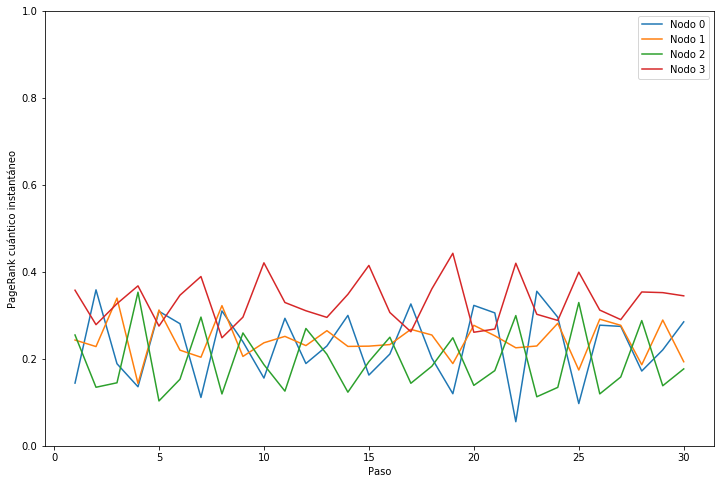
\includegraphics[width=0.9\linewidth]{img/tree-inst-lossless.png}
        \caption{Sin relajación}
    \end{subfigure}
    \begin{subfigure}[m]{0.45\textwidth}
        \centering
        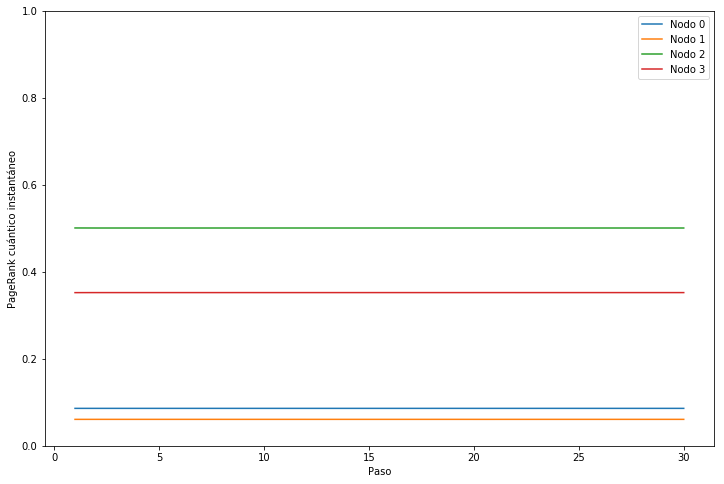
\includegraphics[width=0.9\linewidth]{img/tree-inst-lossy.png}
        \caption{Con relajación}
    \end{subfigure}
    \caption[PageRank cuántico instantaneo del grafo árbol con y sin pérdidas]{PageRank cuántico instantaneo del grafo árbol con y sin pérdidas}
    \label{fig:insttreelossy}
\end{figure}

\begin{figure}[H]
    \centering
    \begin{subfigure}[m]{0.45\textwidth}
        \centering
        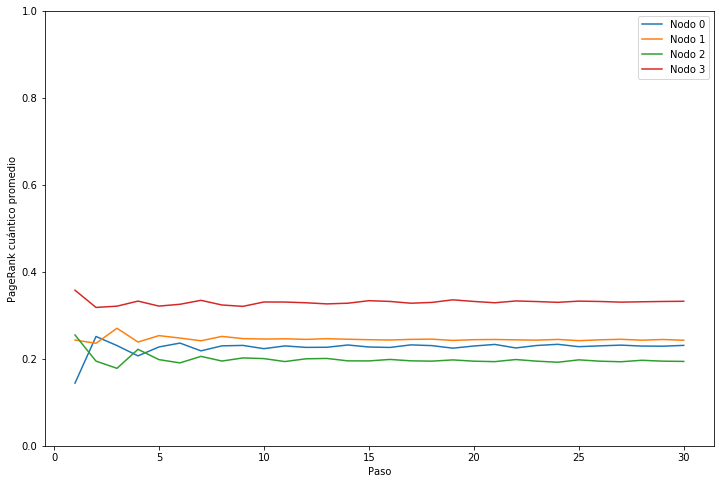
\includegraphics[width=0.9\linewidth]{img/tree-mean-lossless.png}
        \caption{Sin relajación}
    \end{subfigure}
    \begin{subfigure}[m]{0.45\textwidth}
        \centering
        \includegraphics[width=0.9\linewidth]{img/tree-mean-lossy.png}
        \caption{Con relajación}
    \end{subfigure}
    \caption[PageRank cuántico promedio del grafo árbol con y sin pérdidas]{PageRank cuántico promedio del grafo árbol con y sin pérdidas}
    \label{fig:meantreelossy}
\end{figure}

\subsection{Grafo aleatorio}

\begin{equation}
    A =
    \begin{pmatrix}
        0 & 1 & 0 & 0 \\
        1 & 0 & 0 & 0 \\
        1 & 0 & 0 & 1 \\
        1 & 1 & 1 & 0 \\
    \end{pmatrix}
\end{equation}

\begin{equation}
    E =
    \begin{pmatrix}
        0 & \frac{1}{2} & 0 & 0 \\
        \frac{1}{3} & 0 & 0 & 0 \\
        \frac{1}{3} & 0 & 0 & 1 \\
        \frac{1}{3} & \frac{1}{2} & 1 & 0 \\
    \end{pmatrix}
\end{equation}

\begin{equation}
    G =
    \begin{pmatrix}
        \frac{3}{80} & \frac{37}{80} & \frac{3}{80} & \frac{3}{80} \\
        \frac{77}{240} & \frac{3}{80} & \frac{3}{80} & \frac{3}{80} \\
        \frac{77}{240} & \frac{3}{80} & \frac{3}{80} & \frac{71}{80} \\
        \frac{77}{240} & \frac{37}{80} & \frac{71}{80} & \frac{3}{80} \\
    \end{pmatrix}
\end{equation}

\begin{figure}[H]
    \centering
    \includegraphics[width=0.5\linewidth]{img/any.png}
    \caption[Grafo aleatorio]{Grafo aleatorio}
    \label{fig:any}
\end{figure}

\begin{figure}[H]
    \centering
    \begin{subfigure}[m]{0.45\textwidth}
        \centering
        \includegraphics[width=0.9\linewidth]{img/any-inst-M.png}
        \caption{Wolfram Mathematica}
    \end{subfigure}
    \begin{subfigure}[m]{0.45\textwidth}
        \centering
        \includegraphics[width=0.9\linewidth]{img/any-inst-lossless.png}
        \caption{Python}
    \end{subfigure}
    \caption[PageRank cuántico instantáneo del grafo aleatorio sin pérdidas]{PageRank cuántico instantáneo del grafo aleatorio sin pérdidas}
    \label{fig:instanylossless}
\end{figure}

\begin{figure}[H]
    \centering
    \begin{subfigure}[m]{0.45\textwidth}
        \centering
        \includegraphics[width=0.9\linewidth]{img/any-mean-M.png}
        \caption{Wolfram Mathematica}
    \end{subfigure}
    \begin{subfigure}[m]{0.45\textwidth}
        \centering
        \includegraphics[width=0.9\linewidth]{img/any-mean-lossless.png}
        \caption{Python}
    \end{subfigure}
    \caption[PageRank cuántico promedio del grafo aleatorio sin pérdidas]{PageRank cuántico promedio del grafo aleatorio sin pérdidas}
    \label{fig:meananylossless}
\end{figure}

\begin{figure}[H]
    \centering
    \begin{subfigure}[m]{0.45\textwidth}
        \centering
        \includegraphics[width=0.9\linewidth]{img/any-inst-lossless.png}
        \caption{Sin relajación}
    \end{subfigure}
    \begin{subfigure}[m]{0.45\textwidth}
        \centering
        \includegraphics[width=0.9\linewidth]{img/any-inst-lossy.png}
        \caption{Con relajación}
    \end{subfigure}
    \caption[PageRank cuántico instantaneo del grafo aleatorio con y sin pérdidas]{PageRank cuántico instantaneo del grafo aleatorio con y sin pérdidas}
    \label{fig:instanylossy}
\end{figure}

\begin{figure}[H]
    \centering
    \begin{subfigure}[m]{0.45\textwidth}
        \centering
        \includegraphics[width=0.9\linewidth]{img/any-mean-lossless.png}
        \caption{Sin relajación}
    \end{subfigure}
    \begin{subfigure}[m]{0.45\textwidth}
        \centering
        \includegraphics[width=0.9\linewidth]{img/any-mean-lossy.png}
        \caption{Con relajación}
    \end{subfigure}
    \caption[PageRank cuántico promedio del grafo aleatorio con y sin pérdidas]{PageRank cuántico promedio del grafo aleatorio con y sin pérdidas}
    \label{fig:meananylossy}
\end{figure}




\chapter{Conclusiones}

En el presente trabajo se estudiaron las bases de información cuántica, superconductividad, computación cuántica con transmones y tres algoritmos cuánticos. Se construyó un simulador de transmones acoplados a un mismo resonador y el set de instrucciones del procesador cuántico formado por estos transmones. Con este simulador se ejecutaron los tres algoritmos estudiados, los cuales son: El algoritmo de búsqueda de Grover, el algoritmo de factorización de Shor y el algoritmo de centralidad PageRank. Además, las simulaciones se realizaron para un sistema cerrado y para un sistema abierto markoviano.

Del algoritmo de Grover, se realizaron simulaciones del algoritmo con tres bases de datos distintas de dieciséis elementos y un estado marcado, una de dos estados marcados y una de cuatro estados marcados. Con el algoritmo de Shor se factorizaron los números quince y ocho. Luego, el algoritmo PageRank se aplicó a cuatro grafos, uno estrella, uno corona, uno árbol y uno aleatorio.

Debido a que el presente trabajo persiguió objetivos que en nuestra universidad no se dictan dentro del contenido programático de la carrera de Ingeniería Electrónica, se decidió hacer una presentación detallada de los conceptos y herramienta necesarias para la comprensión de la teoría de información cuántica, la computación cuántica superconductora y los algoritmos simulados. Hasta donde conocemos, no existe ningún otro trabajo que haya simulado estos algoritmos en un sistema abierto markoviano y es el primer trabajo de computación cuántica en un departamento de ingeniería venezolano.

En el presente trabajo, se desarrollaron las siguientes herramientas y se obtuvieron los siguientes resultados novedosos:

\begin{enumerate}
    \item Una compuerta controlada de fase CP que permita eliminar las fases en las compuertas de negación con dos o más qubits de control, como la de Toffoli.
    \item Un conjunto de instrucciones cuánticas basadas en las compuertas nativas de los transmones y un simulador del sistema físico.
    \item Un operador de multiplicación por 3 módulo 8 sin qubits de ancilla.
    \item La forma explícita del operador de difusión de las caminatas cuánticas de Szegedy para grafos de cuatro nodos, en función de rotaciones en Y controladas.
    \item El efecto de la relajación en los algoritmos de Grover, Shor y PageRank.
\end{enumerate}

En el algoritmo de Grover se ha visto que con relajación, sólo se puede realizar una iteración. En la segunda ya no se puede garantizar que el estado deseado el de probabilidad más alta y en general tiene probabilidad mayor al final de la primera que al final de la segunda. Así que la mejor alternativa en este algoritmo es su variante de un paso. Sin embargo, debido a que se deben procesar $\Omega(N \log(N))$ medidas, se pierde la ventaja de ejecutar una búsqueda cuántica.

El algoritmo de Shor no se pudo simular con relajación, debido a los largos tiempos que esto hubiese tomado. La ejecución del operador de multiplicación modular $MUL(7,15)$ tomó 72 horas y la del operador $MUL(3,8)$ tomó más de 120 horas. Estos operadores se deben aplicar 15 veces en total, así que el tiempo de ejecución de estas simulaciones hubiese sido de al menos 45 y 75 días, para factorizar los números 15 y 8, respectivamente.

En cuanto al algoritmo PageRank, cada iteración del algoritmo es tan larga, que exceden el tiempo de vida de los qubits y al final de cada iteración sólo se tiene el efecto de las últimas compuertas de esta, se pierde el efecto de las primeras. Como la relajación borra toda la información del inicio de la iteración, todas las iteraciones terminan siendo iguales y se miden los mismos valores al final de cada una.

Los resultados de las simulaciones del algoritmo de Grover y PageRank nos indican que para sistemas con tiempos de relajación del orden de $O(10^4 ns)$, los protocolos de corrección de errores son una necesidad. Este es un resultado significante, pues el record actual de tiempo de vida de un qubit superconductor es inferior a 0.1ms, está en el mismo orden de magnitud que el del sistema simulado.


\part*{Apéndices}
\appendix
\chapter{Cálculos de Hamiltonianos}
\label{ch:hamiltonians}

\section{Régimen rotacional del pulso}

Partiendo del Hamiltoniano de Jaynes-Cummings para un sistema multiqubit con pulsos de microondas bajo la aproximación de onda rotacional:

\begin{equation}
    \hat{H}_1 = \hat{H}_{syst} + \hat{H}_d = \omega_r a^\dag a - \frac{1}{2} \sum\limits_i \omega_{qi} \sigma_{zi} + \sum\limits_i g_i (a \sigma_{+ i} + a^\dagger \sigma_{- i}) + \sum\limits_k a\xi_k^*e^{i\omega_d^{(k)}t}+ a^\dagger\xi_ke^{-i\omega_d^{(k)}t}
\end{equation}

Aplicamos la siguiente transformación unitaria para entrar en el regimen rotacional del pulso aplicado

\begin{equation}
    U(t) = exp[\sum\limits_n-i \omega_d^{(n)} t(a^\dagger a - \frac{1}{2} \sum\limits_i \sigma_{z i})]
\end{equation}

De esta manera, el Hamiltoniano en el régimen rotacional del pulso tendrá la siguiente forma:

\begin{equation}
    \hat{H}_2 = U^\dagger (\hat{H}_{syst} + \hat{H}_d) U - i U^\dagger \dot{U}
\end{equation}

Donde $\dot{U}$ representa la derivada temporal del operador unitario $U$.

Utilizaremos la formula de Baker-Campbell-Hausdorff para calcular este Hamiltoniano, ya que esta nos permite realizar el producto con los exponenciales de operadores calculando sólo conmutadores.

\begin{equation}
    e^{-\lambda X} H e^{\lambda X} = H + \lambda [H,X] + \frac{\lambda^2}{2!}[[H,X],X] + ...
\end{equation}

En cuanto a los conmutadores, podemos utilizar las siguientes identidades:

\begin{align}
    [a, a^\dagger] &= 1
    \label{eq:a_ad} \\
    [a, a^\dagger a] &= a a^\dagger a - a^\dagger a a = (a a^\dagger - a^\dagger a) a = [a, a^\dagger] a = a
    \label{eq:a_ada} \\
    [a^\dagger, a^\dagger a] &= a^\dagger a^\dagger a - a^\dagger a a^\dagger = a^\dagger (a^\dagger a - a a^\dagger) = a^\dagger [a^\dagger, a] = -a^\dagger
    \label{eq:ad_ada} \\
    [\sigma_+, \sigma_z] &= 2 \sigma_+
    \label{eq:sp_sz} \\
    [\sigma_-, \sigma_z] &= - 2 \sigma_-
    \label{eq:sm_sz} \\
    [\sigma_-, \sigma_+] &= \sigma_z
    \label{eq:sm_sp}
\end{align}

Para que el cálculo sea visualmente más manejable, aprovechamos la propiedad distributiva de los conmutadores y separaremos el Hamiltoniano $\hat{H}_1$ en los siguientes términos:

\begin{enumerate}
    \item $\hat{H}_r = \omega_r a^\dag a$
    \item $\hat{H}_q = - \frac{1}{2} \sum\limits_i \omega_{qi} \sigma_{zi}$
    \item $\hat{H}_{qr} = \sum\limits_i g_i (a \sigma_{+ i} + a^\dagger \sigma_{- i})$
    \item $\hat{H}_d = \sum\limits_k (a\xi_k^*e^{i\sum\limits_k \omega_d^{(k)}t}+ a^\dagger\xi_ke^{-i\sum\limits_k \omega_d^{(k)}t})$
\end{enumerate}


Con el primer término tenemos el siguiente conmutador:

\begin{equation}
    [\omega_r a^\dag a, \sum\limits_n-i \omega_d^{(n)} t(a^\dagger a - \frac{1}{2} \sum\limits_i \sigma_{z i})] = 0
\end{equation}

El cual es igual a cero, ya que $a^\dagger a$ conmuta con sí mismo, como todo operador, y con $\sigma_{z_i}$, ya que actúan sobre particiones distintas del sistema.

Con el segundo término tenemos el siguiente conmutador:

\begin{equation}
    [- \frac{1}{2} \sum\limits_i \omega_{qi} \sigma_{zi} , \sum\limits_n-i \omega_d^{(n)} t(a^\dagger a - \frac{1}{2} \sum\limits_i \sigma_{z i})] = 0
\end{equation}

El cual es igual a cero, ya que $\sigma_{z_i}$ conmuta consigo mismo y con $a^\dagger a$.

Con el tercer término tenemos el siguiente conmutador:

\begin{multline}
\left[\sum\limits_i g_i (a \sigma_{+ i} + a^\dagger \sigma_{- i}), \sum\limits_n-i \omega_d^{(n)} t(a^\dagger a - \frac{1}{2} \sum\limits_i \sigma_{z i})\right] = \\
\sum\limits_n-i \omega_d^{(n)} t \left[\sum\limits_i g_i (a \sigma_{+ i} + a^\dagger \sigma_{- i}), (a^\dagger a)\right] \\
+ \sum\limits_n-i \omega_d^{(n)} t \left[\sum\limits_i g_i (a \sigma_{+ i} + a^\dagger \sigma_{- i}), (- \frac{1}{2} \sum\limits_i \sigma_{z i})\right] = \\
\sum\limits_n-i \omega_d^{(n)} t \sum\limits_i g_i (a \sigma_{+ i} - a^\dagger \sigma_{- i})
- \sum\limits_n-i \omega_d^{(n)} t \sum\limits_i g_i (a \sigma_{+ i} - a^\dagger \sigma_{- i}) = 0
\end{multline}

En este caso, utilizamos el hecho de que $a$, $a^\dagger$ y $a^\dagger a$ conmutan con $\sigma_{z_i}$, $\sigma_{+_i}$ y $\sigma_{-_i}$, igual que $\sigma_{z_i}$, $\sigma_{+_i}$ y $\sigma_{-_i}$ con $\sigma_{z_j}$, $\sigma_{+_j}$ y $\sigma_{-_j}$, donde $i \neq j$, ya que actuan sobre particiones distintas. También utilizamos las identidades \ref{eq:a_ad} - \ref{eq:sm_sp} y el hecho de que todo operador conmuta con sí mismo. De esta manera llegamos a una resta de dos términos iguales, así que este conmutador también es cero.

Con el cuarto término tenemos el siguiente conmutador:

\begin{multline}
    \left[\sum\limits_k \left(a\xi_k^*e^{i\sum\limits_k \omega_d^{(k)}t}+ a^\dagger\xi_ke^{-i\sum\limits_k \omega_d^{(k)}t}\right), \sum\limits_n-i \omega_d^{(n)} t\left(a^\dagger a - \frac{1}{2} \sum\limits_i \sigma_{z i}\right)\right] = \\
    \left(\sum\limits_n-i \omega_d^{(n)} t\right) \sum\limits_k \left(a\xi_k^*e^{i\sum\limits_k \omega_d^{(k)}t} - a^\dagger\xi_ke^{-i\sum\limits_k \omega_d^{(k)}t}\right)
\end{multline}

Aquí hemos utilzado el hecho de que $a$ y $a^\dagger$ conmutan con $\sigma_{z_i}$ y las identidades \ref{eq:a_ada} y \ref{eq:ad_ada}. Este conmutador no es igual a cero como los anteriores, así que tenemos que utilizar este resultado para calcular $[[H,X],X]$.

\begin{multline}
    \left[\left(\sum\limits_n-i \omega_d^{(n)} t\right) \sum\limits_k \left(a\xi_k^*e^{i\sum\limits_k \omega_d^{(k)}t} - a^\dagger\xi_ke^{-i\sum\limits_k \omega_d^{(k)}t}\right), \sum\limits_n-i \omega_d^{(n)} t\left(a^\dagger a - \frac{1}{2} \sum\limits_i \sigma_{z i}\right)\right] = \\
    \left(\sum\limits_n-i \omega_d^{(n)} t\right)^2 \sum\limits_k \left(a\xi_k^*e^{i\sum\limits_k \omega_d^{(k)}t} + a^\dagger\xi_ke^{-i\sum\limits_k \omega_d^{(k)}t}\right)
\end{multline}
 
De igual manera que en el conmutador anterior, hemos utilzado el hecho de que $a$ y $a^\dagger$ conmutan con $\sigma_{z_i}$ y las identidades \ref{eq:a_ada} y \ref{eq:ad_ada}. Este conmutador no es igual a cero como los anteriores, así que tenemos que utilizar este resultado para calcular $[[[H,X],X],X]$.

\begin{multline}
    \left[\left(\sum\limits_n-i \omega_d^{(n)} t\right)^2 \sum\limits_k \left(a\xi_k^*e^{i\sum\limits_k \omega_d^{(k)}t}+ a^\dagger\xi_ke^{-i\sum\limits_k \omega_d^{(k)}t}\right), \left(\sum\limits_n-i \omega_d^{(n)} t\right)\left(a^\dagger a - \frac{1}{2} \sum\limits_i \sigma_{z i}\right)\right] = \\
    \left(\sum\limits_n-i \omega_d^{(n)} t\right)^3 \sum\limits_k \left(a\xi_k^*e^{i\sum\limits_k \omega_d^{(k)}t} - a^\dagger\xi_ke^{-i\sum\limits_k \omega_d^{(k)}t}\right)
\end{multline}

De igual manera que en el conmutador anterior, hemos utilzado el hecho de que $a$ y $a^\dagger$ conmutan con $\sigma_{z_i}$ y las identidades \ref{eq:a_ada} y \ref{eq:ad_ada}. Este conmutador no es igual a cero como los anteriores, así que tenemos que utilizar este resultado para calcular $[[[[H,X],X],X],X]$.

\begin{multline}
    \left[\left(\sum\limits_n-i \omega_d^{(n)} t\right)^3 \sum\limits_k \left(a\xi_k^*e^{i\sum\limits_k \omega_d^{(k)}t} - a^\dagger\xi_ke^{-i\sum\limits_k \omega_d^{(k)}t}\right), \left(\sum\limits_n-i \omega_d^{(n)} t\right)\left(a^\dagger a - \frac{1}{2} \sum\limits_i \sigma_{z i}\right)\right] = \\
    \left(\sum\limits_n-i \omega_d^{(n)} t\right)^4 \sum\limits_k \left(a\xi_k^*e^{i\sum\limits_k \omega_d^{(k)}t} + a^\dagger\xi_ke^{-i\sum\limits_k \omega_d^{(k)}t}\right)
\end{multline}

En este punto podemos notar cierto patrón. Esta serie de conmutadores nos recuerda a la serie de Taylor de la función exponencial con argumento $\sum\limits_n-i \omega_d^{(n)} t$. Al sustituirlos en la fórmula de Baker-Campbell-Hausdorff, vemos que efectivamente se trata de este exponencial. Entonces, el primer término del Hamiltoniano $\hat{H}_2$ es:

\begin{equation}
    U^\dagger (\hat{H}_1) U = \hat{H}_{syst} + \sum\limits_k (e^{\sum\limits_n-i \omega_d^{(n)} t} a\xi_k^*e^{\sum\limits_k i\omega_d^{(k)}t}+ e^{-\sum\limits_n-i \omega_d^{(n)} t} a^\dagger\xi_ke^{-\sum\limits_k i\omega_d^{(k)}t}) = \hat{H}_{syst} + \sum\limits_k (a\xi_k^* + a^\dagger\xi_k)
\end{equation}

Por otro lado, el segundo término es:

\begin{equation}
    - i U^\dagger \dot{U} = -i U^\dagger (-i \sum\limits_n \omega_d^{(n)} (a^\dagger a - \frac{1}{2} \sum\limits_i \sigma_{z i})) U = - \sum\limits_n \omega_d^{(n)}(a^\dagger a - \frac{1}{2} \sum\limits_i \sigma_{z i})
\end{equation}

Es decir, $-i$ por la derivada temporal del argumento del exponencial en el que consiste $U$. Esto es porque todo exponencial conmuta con su argumento y en este caso, la derivada interna de U es igual al argumento del exponencial entre el escalar $t$, por lo que también conmuta con U. Además de que como $U$ es unitario, se cumple que $U^\dagger U = \mathds{1}$.

Finalmente, sumando y agrupando términos, nos queda que el Hamiltoniano en el régimen rotacional del pulso es:

\begin{equation}
    \hat{H}_2 = (\omega_r - \sum\limits_n \omega_d^{(n)}) a^\dag a - \frac{1}{2} \sum\limits_i (\omega_{qi} - \sum\limits_n \omega_d^{(n)}) \sigma_{zi} + \sum\limits_i g_i (a \sigma_{+ i} + a^\dagger \sigma_{- i}) + \sum\limits_k (a\xi_k^* + a^\dagger\xi_k)
\end{equation}

En el caso de un pulso de un sólo modo, este Hamiltoniano toma la forma:

\begin{equation}
    \hat{H} = \Delta_r a^\dagger a - \frac{1}{2} \sum\limits_i \Delta_{qi} \sigma_{zi} + \sum\limits_i g_i (a \sigma_{+ i} + a^\dagger \sigma_{- i}) + (a\xi^*+a^\dagger\xi )
\end{equation}

Donde $\Delta_r = \omega_r - \omega_d$ es la diferencia entre la frecuencia de resonancia del resonador y la frecuencia central del pulso, y $\Delta_{qi} = \omega_{qi} - \omega_d$ es la diferencia entre la frecuencia de resonancia de cada qubit y la frecuencia central del pulso.

\section{Efecto del pulso sobre el qubit}

Ahora desplazaremos el campo $a$, aplicando el operador de desplazamineto

\begin{equation}
    D(\alpha) = exp[\alpha a^\dagger - \alpha^* a]
\end{equation}

Al Hamiltoniano $\hat{H}_2$ monomodo, con $\dot{\alpha} = -i \Delta_r \alpha -i \xi$, para eliminar el efecto directo del pulso sobre el resonador y ver cómo afecta a los qubits.

De esta manera, el nuevo Hamiltoniano será:

\begin{equation}
    \hat{H}_3 = D^\dagger (\alpha) \hat{H}_2 D(\alpha) -i D^\dagger(\alpha) \dot{D}(\alpha)
\end{equation}

Los operadores de desplazamiento cumplen con las siguientes propiedades:

\begin{align}
    D(-\alpha) &= D^\dagger(\alpha) = D^{-1}(\alpha) \\
    D^\dagger(\alpha) a D(\alpha) &= a + \alpha \\
    D^\dagger(\alpha) a^\dagger D(\alpha) &= a^\dagger + \alpha^*
\end{align}

Utilizando estas dos propiedes, podemos calcular $D^\dagger(\alpha) \hat{H}_2 D(\alpha)$ directamente sin utilizar la expansión de Baker-Campbell-Hausdorff, pues basta con sustituir $a$ por $a+\alpha$ y $a^\dagger$ por $a^\dagger+\alpha^*$.

\begin{multline}
  D^\dagger(\alpha) \hat{H}_2 D(\alpha) = \Delta_r (a^\dagger + \alpha^*) (a + \alpha) - \frac{1}{2} \sum\limits_i \Delta_{qi} \sigma_{zi} + \sum\limits_i g_i [(a+\alpha) \sigma_{+ i} + (a^\dagger+\alpha^*) \sigma_{- i}] \\
  + [(a+\alpha)\xi^*+(a^\dagger+\alpha^*)\xi]
\end{multline}

Estas mismas propiedades también se utilizan para calcular el otro término de $\hat{H}_3$, de la siguiente manera:

\begin{equation}
    -i D^\dagger(\alpha) \dot{D}(\alpha) = -i D^\dagger(\alpha) (\dot{\alpha} a^\dagger - \dot{\alpha}^* a) D(\alpha) = -i[\dot{\alpha} (a^\dagger + \alpha^*) - \dot{\alpha}^* (a + \alpha)]
\end{equation}

Finalemente, sumando, sustituyendo $\dot{\alpha}$ y agrupando, nos queda:

\begin{equation}
    \hat{H}_3 = \Delta_r a^\dagger a - \frac{1}{2} \sum\limits_i \Delta_{qi} \sigma_{zi} + \sum\limits_i g_i (a \sigma_{+i} + a^\dagger \sigma_{-i}) + \sum\limits_i g_i (\alpha \sigma_{+i} + \alpha^* \sigma_{-i}) - \Delta_c \alpha \alpha^*
\end{equation}

El término $-\Delta_r \alpha \alpha^*$ se desprecia, ya que sólo representa una fase global en la evolución del sistema.

\section{Régimen dispersivo}

Finalmente, aplicamos la transformación

\begin{equation}
    U = exp[\sum\limits_i \frac{g_i} {\Delta_i} (a^\dagger \sigma_{-i} - a \sigma_{+i})]
\end{equation}

Donde $\Delta_i = \omega_{qi} - \omega_r$ y realizamos la expansión de Baker-Campbell-Hausdorff de segundo grado sobre los términos $\frac{g_i}{\Delta_i} \ll 1$. El Hamiltoniano efectivo $\hat{H}_{eff}$ será la aproximación del Hamiltoniano $\hat{H}_4$ resultante de esta expansión.

\begin{equation}
    \hat{H}_{eff} \approx \hat{H}_4 = U^\dagger \hat{H}_3 U
\end{equation}

Para resolver los conmutadores seguiremos el esquema utilizado anteriormente y separaremos el Hamiltoniano $\hat{H}_3$ en los siguientes términos:

\begin{enumerate}
    \item $\hat{H}_r = \Delta_r a^\dagger a$
    \item $\hat{H}_q = - \frac{1}{2} \sum\limits_i \Delta_{qi} \sigma_{zi}$
    \item $\hat{H}_{qr} = \sum\limits_i g_i (a \sigma_{+i} + a^\dagger \sigma_{-i})$
    \item $\hat{H}_d = \sum\limits_i g_i (\alpha \sigma_{+i} + \alpha^* \sigma_{-i})$
\end{enumerate}

Con el primer término tenemos el siguiente conmutador:

\begin{equation}
    [\Delta_r a^\dagger a, \sum\limits_i \frac{g_i} {\Delta_i} (a^\dagger \sigma_{-i} - a \sigma_{+i})] = \Delta_r \sum\limits_i \frac{g_i} {\Delta_i} (a^\dagger \sigma_{-i} + a \sigma_{+i})
\end{equation}

Con el segundo término tenemos el siguiente conmutador:

\begin{equation}
    [- \frac{1}{2} \sum\limits_i \Delta_{qi} \sigma_{zi}, \sum\limits_i \frac{g_i} {\Delta_i} (a^\dagger \sigma_{-i} - a \sigma_{+i})] = - \sum\limits_i \frac{g_i} {\Delta_i} \Delta_{qi} (a^\dagger \sigma_{-i} + a \sigma_{+i})
\end{equation}

Con el tercer término tenemos el siguiente conmutador:

\begin{multline}
[\sum\limits_i g_i (a \sigma_{+i} + a^\dagger \sigma_{-i}), \sum\limits_j \frac{g_j} {\Delta_j} (a^\dagger \sigma_{-j} - a \sigma_{+j})] = \\
\sum\limits_{ij} g_i \frac{g_j}{\Delta_j} \left([ a \sigma_{+i}, a^\dagger \sigma_{-j}] +
[a \sigma_{+i}, - a \sigma_{+j}] +
[a^\dagger \sigma_{-i}, a^\dagger \sigma_{-j}] +
[a^\dagger \sigma_{-i}, - a \sigma_{+j}]\right) =\\
\sum\limits_{ij} g_i \frac{g_j}{\Delta_j} \left([ a \sigma_{+i}, a^\dagger \sigma_{-j}] +
[a^\dagger \sigma_{-i}, - a \sigma_{+j}]\right) =\\
\sum\limits_{ij} g_i \frac{g_j}{\Delta_j} \left(
    a \sigma_{+i} a^\dagger \sigma_{-j} - a^\dagger \sigma_{-j} a \sigma_{+i}
    - a^\dagger \sigma_{-i} a \sigma_{+j} + a \sigma_{+j} a^\dagger \sigma_{-i}\right) =\\
\sum\limits_{ij} g_i \frac{g_j}{\Delta_j} \left(
    a a^\dagger \sigma_{+i} \sigma_{-j} - a^\dagger a \sigma_{-j} \sigma_{+i}
    - a^\dagger a \sigma_{-i} \sigma_{+j} + a a^\dagger \sigma_{+j} \sigma_{-i}\right) =\\
\sum\limits_{ij} g_i \frac{g_j}{\Delta_j} \left(
    (1 + a^\dagger a) \sigma_{+i} \sigma_{-j} - a^\dagger a \sigma_{-j} \sigma_{+i}
    - a^\dagger a \sigma_{-i} \sigma_{+j} + (1 + a^\dagger a) \sigma_{+j} \sigma_{-i}\right) =\\
\sum\limits_{ij} g_i \frac{g_j}{\Delta_j} \left(
    \sigma_{+i} \sigma_{-j} + a^\dagger a \sigma_{+i} \sigma_{-j} - a^\dagger a \sigma_{-j} \sigma_{+i}
    - a^\dagger a \sigma_{-i} \sigma_{+j} + \sigma_{+j} \sigma_{-i} + a^\dagger a \sigma_{+j} \sigma_{-i}\right) =\\
\sum\limits_{ij} g_i \frac{g_j}{\Delta_j} \left(\sigma_{+i} \sigma_{-j} + \sigma_{+j} \sigma_{-i}\right) +
\sum\limits_{ij} g_i \frac{g_j}{\Delta_j} a^\dagger a \left(
    \sigma_{+i} \sigma_{-j} - \sigma_{-j} \sigma_{+i}
    - \sigma_{-i} \sigma_{+j} + \sigma_{+j} \sigma_{-i}\right) =\\
\sum\limits_{ij} g_i \frac{g_j}{\Delta_j} \left(\sigma_{+i} \sigma_{-j} + \sigma_{+j} \sigma_{-i}\right) -
2 \sum\limits_{i} \frac{g_i^2}{\Delta_i} a^\dagger a \sigma_{zi}
\end{multline}

Con el cuarto término tenemos el siguiente conmutador:

\begin{multline}
[\sum\limits_i g_i (\alpha \sigma_{+i} + \alpha^* \sigma_{-i}), \sum\limits_i \frac{g_i} {\Delta_i} (a^\dagger \sigma_{-i} - a \sigma_{+i})] =\\
\sum\limits_{ij} g_i \frac{g_j} {\Delta_j} \left([\alpha \sigma_{+i}, a^\dagger \sigma_{-j}] - [\alpha^* \sigma_{-i}, a \sigma_{+j}]\right) =
- \sum\limits_i \frac{g_i^2} {\Delta_i} (\alpha a^\dagger + \alpha^* a) \sigma_{zi}
\end{multline}

-----------------------------------------------------------


Con el primer término tenemos el siguiente conmutador:

\begin{multline}
    [\Delta_r \sum\limits_i \frac{g_i} {\Delta_i} (a^\dagger \sigma_{-i} + a \sigma_{+i}), \sum\limits_j \frac{g_j} {\Delta_j} (a^\dagger \sigma_{-j} - a \sigma_{+j})] = \\
    \Delta_r \sum\limits_{ij} \frac{g_i g_j}{\Delta_i \Delta_j} \left([(a^\dagger \sigma_{-i} ), (- a \sigma_{+j})] + 
        [(a \sigma_{+i}), (a^\dagger \sigma_{-j} )]\right) = \\
\Delta_r \left(\sum\limits_{ij} \frac{g_i g_j}{\Delta_i \Delta_j} \left(\sigma_{+i} \sigma_{-j} + \sigma_{+j} \sigma_{-i}\right) -
2 \sum\limits_{i} \frac{g_i^2}{\Delta_i^2} a^\dagger a \sigma_{zi} \right)
\end{multline}

Con el segundo término tenemos el siguiente conmutador:

\begin{multline}
    [- \sum\limits_i \frac{g_i} {\Delta_i} \Delta_{qi} (a^\dagger \sigma_{-i} + a \sigma_{+i}), \sum\limits_j \frac{g_j} {\Delta_j} (a^\dagger \sigma_{-j} - a \sigma_{+j})] = \\
- \sum\limits_{ij} \Delta_{qi}  \frac{g_i g_j}{\Delta_i \Delta_j} \left(\sigma_{+i} \sigma_{-j} + \sigma_{+j} \sigma_{-i}\right) +
2 \sum\limits_{i} \Delta_{qi} \frac{g_i^2}{\Delta_i^2} a^\dagger a \sigma_{zi}
\end{multline}

Con el tercer término tenemos el siguiente conmutador:

\begin{multline}
[\sum\limits_{ij} g_i \frac{g_j}{\Delta_j} \left(\sigma_{+i} \sigma_{-j} + \sigma_{+j} \sigma_{-i}\right), \sum\limits_k \frac{g_k} {\Delta_k} (a^\dagger \sigma_{-k} - a \sigma_{+k})] = \\
[\sum\limits_{i \neq j} g_i \frac{g_j}{\Delta_j} \left(\sigma_{+i} \sigma_{-j} + \sigma_{+j} \sigma_{-i}\right), \sum\limits_k \frac{g_k} {\Delta_k} (a^\dagger \sigma_{-k} - a \sigma_{+k})] = \\
\sum\limits_{i \neq j, k} g_i \frac{g_j}{\Delta_j} \frac{g_k}{\Delta_k} \left(
[\sigma_{+i} \sigma_{-j},  a^\dagger \sigma_{-k}] +
[\sigma_{+i} \sigma_{-j},  - a \sigma_{+k}] +
[\sigma_{+j} \sigma_{-i},  a^\dagger \sigma_{-k}] +
[\sigma_{+j} \sigma_{-i}, - a \sigma_{+k}] \right) = \\
\sum\limits_{i \neq j} g_i \frac{g_j}{\Delta_j} \left(
[\sigma_{+i} \sigma_{-j}, \frac{g_i}{\Delta_i}  a^\dagger \sigma_{-i}] -
[\sigma_{+i} \sigma_{-j}, \frac{g_j}{\Delta_j} a \sigma_{+j}] +
[\sigma_{+j} \sigma_{-i}, \frac{g_j}{\Delta_j} a^\dagger \sigma_{-j}] -
[\sigma_{+j} \sigma_{-i}, \frac{g_i}{\Delta_i} a \sigma_{+i}] \right) = \\
\sum\limits_{i \neq j} g_i \frac{g_j}{\Delta_j} \left(
- \frac{g_i}{\Delta_i} a^\dagger \sigma_{zi} \sigma_{-j}
- \frac{g_j}{\Delta_j} a \sigma_{+i} \sigma_{zj}
- \frac{g_j}{\Delta_j} a^\dagger \sigma_{zj} \sigma_{-i}
- \frac{g_i}{\Delta_i} a \sigma_{+j} \sigma_{zi} \right)
\end{multline}

\begin{multline}
[- 2 \sum\limits_{i} \frac{g_i^2}{\Delta_i} a^\dagger a \sigma_{zi}, \sum\limits_j \frac{g_j} {\Delta_j} (a^\dagger \sigma_{-j} - a \sigma_{+j})] =
- 2 \sum\limits_{ij} \frac{g_i^2}{\Delta_i} \frac{g_j}{\Delta_j} \left(
[a^\dagger a \sigma_{zi}, a^\dagger \sigma_{-j}] -
[a^\dagger a \sigma_{zi}, a \sigma_{+j}]
\right) = \\
- 2 \sum\limits_{i} \frac{g_i^3}{\Delta_i^2} \left(
(a^\dagger a \sigma_{zi} a^\dagger \sigma_{-i} - a^\dagger \sigma_{-i} a^\dagger a \sigma_{zi}) -
(a^\dagger a \sigma_{zi} a \sigma_{+i} - a \sigma_{+i} a^\dagger a \sigma_{zi})
\right) \\
- 2 \sum\limits_{i \neq j} \frac{g_i^2}{\Delta_i} \frac{g_j}{\Delta_j} \left(
\sigma_{zi} [a^\dagger a, a^\dagger] \sigma_{-j} -
\sigma_{zi} [a^\dagger a, a] \sigma_{+j}
\right) = \\
- 2 \sum\limits_{i} \frac{g_i^3}{\Delta_i^2} \left(
(a^\dagger a \sigma_{zi} a^\dagger \sigma_{-i} - a^\dagger \sigma_{-i} a^\dagger a \sigma_{zi}) -
(a^\dagger a \sigma_{zi} a \sigma_{+i} - a \sigma_{+i} a^\dagger a \sigma_{zi})
\right) \\
- 2 \sum\limits_{i \neq j} \frac{g_i^2}{\Delta_i} \frac{g_j}{\Delta_j} \left(
\sigma_{zi} a^\dagger \sigma_{-j} +
\sigma_{zi} a \sigma_{+j}
\right) = \\
- 2 \sum\limits_{i} \frac{g_i^3}{\Delta_i^2} \left(
(a^\dagger \sigma_{zi} \sigma_{-i} (1 + a^\dagger a) - a^\dagger \sigma_{-i} \sigma_{zi} a^\dagger a) -
(a^\dagger a \sigma_{zi} \sigma_{+i} a - (1 + a^\dagger a) \sigma_{+i} \sigma_{zi} a)
\right) \\
- 2 \sum\limits_{i \neq j} \frac{g_i^2}{\Delta_i} \frac{g_j}{\Delta_j} \left(
\sigma_{zi} a^\dagger \sigma_{-j} +
\sigma_{zi} a \sigma_{+j}
\right) = \\
- 2 \sum\limits_{i} \frac{g_i^3}{\Delta_i^2} \left(
(a^\dagger \sigma_{zi} \sigma_{-i} + a^\dagger (2 \sigma_{-i}) a^\dagger a) -
(a^\dagger a (-2) \sigma_{+i} a - \sigma_{+i} \sigma_{zi} a)
\right) \\
- 2 \sum\limits_{i \neq j} \frac{g_i^2}{\Delta_i} \frac{g_j}{\Delta_j} \left(
\sigma_{zi} a^\dagger \sigma_{-j} +
\sigma_{zi} a \sigma_{+j}
\right)
\end{multline}

Sumando, agrupando y descartando los términos $\sigma_z \sigma_-$, $a^\dagger a \sigma_-$, $\sigma_z (a + a^\dagger)$, sus conjugados hermíticos y otros términos de orden superior, nos queda:

\begin{multline}
[[H,X],X] \approx \Delta_r \left(\sum\limits_{ij} \frac{g_i g_j}{\Delta_i \Delta_j} \left(\sigma_{+i} \sigma_{-j} + \sigma_{+j} \sigma_{-i}\right) -
2 \sum\limits_{i} \frac{g_i^2}{\Delta_i^2} a^\dagger a \sigma_{zi} \right) + \\
- \sum\limits_{ij} \Delta_{qi}  \frac{g_i g_j}{\Delta_i \Delta_j} \left(\sigma_{+i} \sigma_{-j} + \sigma_{+j} \sigma_{-i}\right) +
2 \sum\limits_{i} \Delta_{qi} \frac{g_i^2}{\Delta_i^2} a^\dagger a \sigma_{zi} = \\
- \left(\sum\limits_{ij} \frac{g_i g_j}{\Delta_j} \left(\sigma_{+i} \sigma_{-j} + \sigma_{+j} \sigma_{-i}\right) -
2 \sum\limits_{i} \frac{g_i^2}{\Delta_i} a^\dagger a \sigma_{zi} \right) \\
\end{multline}

\begin{multline}
    [H,X] = \Delta_r \sum\limits_i \frac{g_i} {\Delta_i} (a^\dagger \sigma_{-i} + a \sigma_{+i}) - \sum\limits_i \frac{g_i} {\Delta_i} \Delta_{qi} (a^\dagger \sigma_{-i} + a \sigma_{+i}) \\
+ \sum\limits_{ij} g_i \frac{g_j}{\Delta_j} \left(\sigma_{+i} \sigma_{-j} + \sigma_{+j} \sigma_{-i}\right) - 2 \sum\limits_{i} \frac{g_i^2}{\Delta_i} a^\dagger a \sigma_{zi} - \sum\limits_i \frac{g_i^2} {\Delta_i} = \\
- \sum\limits_i g_i (a^\dagger \sigma_{-i} + a \sigma_{+i}) + \sum\limits_{ij} g_i \frac{g_j}{\Delta_j} \left(\sigma_{+i} \sigma_{-j} + \sigma_{+j} \sigma_{-i}\right) - 2 \sum\limits_{i} \frac{g_i^2}{\Delta_i} a^\dagger a \sigma_{zi} - \sum\limits_i \frac{g_i^2} {\Delta_i}
\end{multline}

Entonces, sumando y agrupando todos los términos restantes, nos queda:

\begin{multline}
\hat{H}_4 \approx \Delta_r a^\dagger a - \frac{1}{2} \sum\limits_i \Delta_{qi} \sigma_{zi} + \sum\limits_i g_i (a \sigma_{+i} + a^\dagger \sigma_{-i}) + \sum\limits_i g_i (\alpha \sigma_{+i} + \alpha^* \sigma_{-i}) + \\
- \sum\limits_i g_i (a^\dagger \sigma_{-i} + a \sigma_{+i}) + \sum\limits_{ij} \frac{g_i g_j}{\Delta_j} \left(\sigma_{+i} \sigma_{-j} + \sigma_{+j} \sigma_{-i}\right) - 2 \sum\limits_{i} \frac{g_i^2}{\Delta_i} a^\dagger a \sigma_{zi} \\
- \frac{1}{2} \left(\sum\limits_{ij} \frac{g_i g_j}{\Delta_j} \left(\sigma_{+i} \sigma_{-j} + \sigma_{+j} \sigma_{-i}\right) -
2 \sum\limits_{i} \frac{g_i^2}{\Delta_i} a^\dagger a \sigma_{zi} \right) = \\
(\Delta_r - \sum\limits_{i} \frac{g_i^2}{\Delta_i} \sigma_{zi}) a^\dagger a - \frac{1}{2} \sum\limits_i \Delta_{qi} \sigma_{zi} + \sum\limits_i g_i (a \sigma_{+i} + a^\dagger \sigma_{-i}) + \sum\limits_i g_i (\alpha \sigma_{+i} + \alpha^* \sigma_{-i}) + \\
\sum\limits_{ij} \frac{g_i g_j}{2 \Delta_j} \left(\sigma_{+i} \sigma_{-j} + \sigma_{+j} \sigma_{-i}\right)
\end{multline}

\begin{multline}
\hat{H}_{eff} = \tilde{\Delta}_r a^\dagger a - \frac{1}{2} \sum\limits_i \Delta_{qi} \sigma_{zi} + \sum\limits_i g_i (a \sigma_{+i} + a^\dagger \sigma_{-i}) + \sum\limits_i g_i (\alpha \sigma_{+i} + \alpha^* \sigma_{-i}) + \\
\sum\limits_{ij} \frac{g_i g_j}{2 \Delta_j} \left(\sigma_{+i} \sigma_{-j} + \sigma_{+j} \sigma_{-i}\right) - \sum\limits_{i} \frac{g_i^2}{\Delta_i} a^\dagger a \sigma_{zi}
\end{multline}




En el caso de dos qubits tenemos:

\begin{equation}
\hat{H}_{eff} \approx \Delta_r a^\dagger a - \frac{1}{2} \sum\limits_i \tilde{\Delta}_{qi} \sigma_{zi} + \sum\limits_i (\Omega_i \sigma_{+i} + \Omega_i^* \sigma_{-i})
+ \frac{g_1 g_2 (\Delta_1 + \Delta_2)}{2 \Delta_1 \Delta_2} (\sigma_{-1} \sigma_{+2}+\sigma_{+1} \sigma_{-2})
\end{equation}

$\tilde{\Delta}_r = (\omega_r - \frac{1}{2} \sum\limits_i \chi_i \sigma_{zi}) - \omega_d \qquad \chi_i = \frac{g_i^2}{\Delta_i}$





-----------------------------------------------------------


% Dr = wr - wd
% Dqi = wqi - wd
% Di = wqi - wr
% Desaparece el acoplamiento resonador-qubits
% Aparece acoplamiento qubit-qubit


%\chapter{Cálculos de matrices de adyacencia}



%\chapter{Circuitos cuánticos}

Rotaciones en Z:

\[
\Qcircuit @C=1.4em @R=1.8em {
& \qw & \gate{Rz({\theta})} & \qw 
}\]
\[\Qcircuit @C=1.4em @R=1.8em {
& \qw & \gate{Ry(\frac{\pi}{2})} & \gate{Rx({\theta})} & \gate{Ry(\frac{-\pi}{2})} & \qw 
}
\]

Compuerta X:

\[
\Qcircuit @C=1.4em @R=1.8em {
& \qw & \gate{X} & \qw 
}\]
\[\Qcircuit @C=1.4em @R=1.8em {
& \qw & \gate{Rx({\pi})} & \qw 
}
\]

Compuerta Y:

\[
\Qcircuit @C=1.4em @R=1.8em {
& \qw & \gate{Y} & \qw 
}\]
\[\Qcircuit @C=1.4em @R=1.8em {
& \qw & \gate{Ry({\pi})} & \qw 
}
\]

Compuerta Z:

\[
\Qcircuit @C=1.4em @R=1.8em {
& \qw & \gate{Z} & \qw 
}\]
\[\Qcircuit @C=1.4em @R=1.8em {
& \qw & \gate{Rz({\pi})} & \qw 
}
\]

Compuerta H:

\[
\Qcircuit @C=1.4em @R=1.8em {
& \qw & \gate{H} & \qw 
}\]
\[\Qcircuit @C=1.4em @R=1.8em {
& \qw & \gate{Ry(\frac{\pi}{2})} & \gate{X} & \qw 
}
\]

Compuerta CNOT:

\[
\Qcircuit @C=1.4em @R=1.8em {
& \qw & \ctrl{1} & \qw \\
& \qw & \targ    & \qw 
}\]
\[
\Qcircuit @C=0.4em @R=0.6em {
& \qw & \qw & \gate{Rz(\frac{-\pi}{2})} & \multigate{1}{\text{iSWAP}} & \gate{H} & \multigate{1}{\text{iSWAP}} & \qw  & \multigate{1}{\text{iSWAP}} &  \gate{Rx(\frac{\pi}{2})} &\multigate{1}{\text{iSWAP}} & \qw & \qw \\
& \qw & \gate{H} & \gate{Rz(\frac{-\pi}{2})} & \ghost{\text{iSWAP}} & \qw & \ghost{\text{iSWAP}}  & \gate{Rx(\frac{-\pi}{2})} & \ghost{\text{iSWAP}} & \qw & \ghost{\text{iSWAP}} & \gate{Rx(\frac{\pi}{2})} & \qw
}
\]


Compuerta CRy:

Tomado del paper de Barenco \cite{barenco}

\[
\Qcircuit @C=1.4em @R=1.8em {
& \qw & \ctrl{1} & \qw \\
& \qw & \gate{Ry(\theta)} & \qw 
}\]
\[\Qcircuit @C=1.4em @R=1.8em {
& \qw & \qw                         & \ctrl{1} & \qw                          & \ctrl{1} & \qw \\
& \qw & \gate{Ry(\frac{\theta}{2})} & \targ    & \gate{Ry(\frac{-\theta}{2})} & \targ    & \qw 
} 
\]

Compuerta CRz:

\[
\Qcircuit @C=1.4em @R=1.8em {
& \qw & \ctrl{1} & \qw \\
& \qw & \gate{Rz(\theta)} & \qw 
}\]
\[\Qcircuit @C=1.4em @R=1.8em {
& \qw & \qw                         & \ctrl{1} & \qw                          & \ctrl{1} & \qw \\
& \qw & \gate{Rz(\frac{\theta}{2})} & \targ    & \gate{Rz(\frac{-\theta}{2})} & \targ    & \qw 
} 
\]

Compuerta SWAP:

\[
\Qcircuit @C=1.4em @R=1.8em {
& \qw & \qswap     & \qw \\
& \qw & \qswap\qwx & \qw 
}\]
\[\Qcircuit @C=1.4em @R=1.8em {
& \qw & \ctrl{1} & \targ     & \ctrl{1} & \qw \\
& \qw & \targ    & \ctrl{-1} & \targ    & \qw 
} 
\]

Compuerta CH:

\[
\Qcircuit @C=1.4em @R=1.8em {
& \qw & \ctrl{1} & \qw \\
& \qw & \gate{H} & \qw 
}\]
\[\Qcircuit @C=1.4em @R=1.8em {
& \qw & \qw                         & \ctrl{1} & \qw                          & \qw \\
& \qw & \gate{Ry(\frac{\theta}{2})} & \targ    & \gate{Ry(\frac{-\theta}{2})} & \qw 
} 
\]

Compuerta $CR^\theta$ blanca:

\[
\Qcircuit @C=1.4em @R=1.8em {
& \qw & \ctrlo{1} & \qw \\
& \qw & \gate{R^\theta} & \qw 
}\]
\[\Qcircuit @C=1.4em @R=1.8em {
& \qw & \gate{Rz(\frac{-3\theta}{4})} & \ctrl{1}                    & \gate{Rz(\frac{\theta}{2})} & \qw \\
& \qw & \gate{Rz(\frac{-3\theta}{4})} & \gate{Rz(\frac{\theta}{2})} & \ctrl{-1}                    & \qw 
} 
\]

Compuerta $CR_\theta$ blanca:

\[
\Qcircuit @C=1.4em @R=1.8em {
& \qw & \ctrlo{1} & \qw \\
& \qw & \gate{R_\theta} & \qw 
}\]
\[\Qcircuit @C=1.4em @R=1.8em {
& \qw & \gate{Rz(\frac{-3\theta}{4})} & \ctrl{1}                    & \gate{Rz(\frac{\theta}{2})} & \qw \\
& \qw & \gate{Rz(\frac{5\theta}{4})} & \gate{Rz(\frac{-3\theta}{2})} & \ctrl{-1}                   & \qw 
} 
\]

Compuerta $CR^\theta$ negra:

\[
\Qcircuit @C=1.4em @R=1.8em {
& \qw & \ctrl{1} & \qw \\
& \qw & \gate{R^\theta} & \qw 
}\]
\[\Qcircuit @C=1.4em @R=1.8em {
& \qw & \gate{Rz(\frac{\theta}{4})} & \ctrl{1}                    & \gate{Rz(\frac{\theta}{2})} & \qw \\
& \qw & \gate{Rz(\frac{\theta}{4})} & \gate{Rz(\frac{-3\theta}{2})} & \ctrl{-1}                  & \qw 
} 
\]

Compuerta $CR_\theta$ negra:

\[
\Qcircuit @C=1.4em @R=1.8em {
& \qw & \ctrl{1}        & \qw \\
& \qw & \gate{R_\theta} & \qw 
}\]
\[\Qcircuit @C=1.4em @R=1.8em {
& \qw & \gate{Rz(\frac{\theta}{4})} & \ctrl{1}                    & \gate{Rz(\frac{\theta}{2})} & \qw \\
& \qw & \gate{Rz(\frac{\theta}{4})} & \gate{Rz(\frac{\theta}{2})} & \ctrl{-1}                    & \qw 
} 
\]

Compuerta de Toffoli (CCNOT):

\[
\Qcircuit @C=1.4em @R=1.8em {
& \qw & \ctrl{1} & \qw \\
& \qw & \ctrl{1} & \qw \\
& \qw & \targ    & \qw 
}\]
\[\Qcircuit @C=1.4em @R=1.8em {
& \qw & \qw      & \qw                       & \ctrl{1} & \qw                      & \ctrl{1} & \ctrl{2}                  & \qw & \ctrl{1}          & \qw \\
& \qw & \qw      & \ctrl{1}                  & \targ    & \ctrl{1}                 & \targ    & \qw                       & \qw & \gate{R_{-\frac{\pi}{2}}} & \qw \\
& \qw & \gate{H} & \gate{Rz(\frac{-\pi}{2})} & \qw      & \gate{Rz(\frac{\pi}{2})} & \qw      & \gate{Rz(\frac{-\pi}{2})} & \gate{H} & \qw & \qw 
} 
\]

Compuerta CCRz:

\[
\Qcircuit @C=1.4em @R=1.8em {
& \qw & \ctrl{1} & \qw \\
& \qw & \ctrl{1} & \qw \\
& \qw & \gate{Rz(\theta)}    & \qw 
}\]
\[\Qcircuit @C=1.4em @R=1.8em {
& \qw & \qw                       & \ctrl{1} & \qw                      & \ctrl{1} & \ctrl{2}                  & \qw \\
& \qw & \ctrl{1}                  & \targ    & \ctrl{1}                 & \targ    & \qw                       & \qw \\
& \qw & \gate{Rz(\frac{\theta}{2})} & \qw      & \gate{Rz(\frac{-\theta}{2})} & \qw      & \gate{Rz(\frac{\theta}{2})} & \qw 
} 
\]

Compuerta CCRy:

\[
\Qcircuit @C=1.4em @R=1.8em {
& \qw & \ctrl{1} & \qw \\
& \qw & \ctrl{1} & \qw \\
& \qw & \gate{Ry(\theta)}    & \qw 
}\]
\[\Qcircuit @C=1.4em @R=1.8em {
& \qw & \qw                       & \ctrl{1} & \qw                      & \ctrl{1} & \ctrl{2}                  & \qw \\
& \qw & \ctrl{1}                  & \targ    & \ctrl{1}                 & \targ    & \qw                       & \qw \\
& \qw & \gate{Ry(\frac{\theta}{2})} & \qw      & \gate{Ry(\frac{-\theta}{2})} & \qw      & \gate{Ry(\frac{\theta}{2})} & \qw 
} 
\]

Compuerta $CCR^\theta$ blanca:

\[
\Qcircuit @C=1.4em @R=1.8em {
& \qw & \ctrlo{1} & \qw \\
& \qw & \ctrlo{1} & \qw \\
& \qw & \gate{R^\theta}    & \qw 
}\]
\[\Qcircuit @C=1.4em @R=1.8em {
& \qw & \qw                       & \ctrlo{1} & \qw                      & \ctrlo{1} & \ctrlo{2}                  & \qw \\
& \qw & \ctrlo{1}                  & \targ    & \ctrlo{1}                 & \targ    & \qw                       & \qw \\
& \qw & \gate{R^\frac{\theta}{2}} & \qw      & \gate{R^\frac{-\theta}{2}} & \qw      & \gate{R^\frac{\theta}{2}} & \qw 
} 
\]

Compuerta $CCR_\theta$ blanca:

\[
\Qcircuit @C=1.4em @R=1.8em {
& \qw & \ctrlo{1} & \qw \\
& \qw & \ctrlo{1} & \qw \\
& \qw & \gate{R_\theta}    & \qw 
}\]
\[\Qcircuit @C=1.4em @R=1.8em {
& \qw & \qw                       & \ctrlo{1} & \qw                      & \ctrlo{1} & \ctrlo{2}                  & \qw \\
& \qw & \ctrlo{1}                  & \targ    & \ctrlo{1}                 & \targ    & \qw                       & \qw \\
& \qw & \gate{R_\frac{\theta}{2}} & \qw      & \gate{R_\frac{-\theta}{2}} & \qw      & \gate{R_\frac{\theta}{2}} & \qw 
} 
\]

Compuerta $CCR^\theta$ negra:

\[
\Qcircuit @C=1.4em @R=1.8em {
& \qw & \ctrl{1} & \qw \\
& \qw & \ctrl{1} & \qw \\
& \qw & \gate{R^\theta}    & \qw 
}\]
\[\Qcircuit @C=1.4em @R=1.8em {
& \qw & \qw                       & \ctrl{1} & \qw                      & \ctrl{1} & \ctrl{2}                  & \qw \\
& \qw & \ctrl{1}                  & \targ    & \ctrl{1}                 & \targ    & \qw                       & \qw \\
& \qw & \gate{R^\frac{\theta}{2}} & \qw      & \gate{R^\frac{-\theta}{2}} & \qw      & \gate{R^\frac{\theta}{2}} & \qw 
} 
\]

Compuerta $CCR_\theta$ negra:

\[
\Qcircuit @C=1.4em @R=1.8em {
& \qw & \ctrl{1} & \qw \\
& \qw & \ctrl{1} & \qw \\
& \qw & \gate{R_\theta}    & \qw 
}\]
\[\Qcircuit @C=1.4em @R=1.8em {
& \qw & \qw                       & \ctrl{1} & \qw                      & \ctrl{1} & \ctrl{2}                  & \qw \\
& \qw & \ctrl{1}                  & \targ    & \ctrl{1}                 & \targ    & \qw                       & \qw \\
& \qw & \gate{R_\frac{\theta}{2}} & \qw      & \gate{R_\frac{-\theta}{2}} & \qw      & \gate{R_\frac{\theta}{2}} & \qw 
} 
\]

Compuerta CCCNOT:

\[
\Qcircuit @C=1.4em @R=1.8em {
& \qw & \ctrl{1} & \qw \\
& \qw & \ctrl{1} & \qw \\
& \qw & \ctrl{1} & \qw \\
& \qw & \targ    & \qw 
}\]
\[\Qcircuit @C=1.4em @R=1.8em {
& \qw & \qw      & \qw                       & \ctrl{1} & \qw                      & \ctrl{1} & \ctrl{2}                  & \qw      & \ctrl{1}                  & \qw \\
& \qw & \qw      & \ctrl{1}                  & \targ    & \ctrl{1}                 & \targ    & \qw                       & \qw      & \ctrl{1}                  & \qw \\
& \qw & \qw      & \ctrl{1}                  & \qw      & \ctrl{1}                 & \qw      & \ctrl{1}                  & \qw      & \gate{R_\frac{-\pi}{2}} & \qw \\
& \qw & \gate{H} & \gate{Rz(\frac{-\pi}{2})} & \qw      & \gate{Rz(\frac{\pi}{2})} & \qw      & \gate{Rz(\frac{-\pi}{2})} & \gate{H} & \qw                       & \qw 
} 
\]

Compuerta CCCRy:

\[
\Qcircuit @C=1.4em @R=1.8em {
& \qw & \ctrl{1} & \qw \\
& \qw & \ctrl{1} & \qw \\
& \qw & \ctrl{1} & \qw \\
& \qw & \gate{Ry(\theta)} & \qw 
}\]
\[\Qcircuit @C=1.4em @R=1.8em {
& \qw & \qw                         & \ctrl{1} & \qw                          & \ctrl{1} & \ctrl{1}                    & \qw \\
& \qw & \qw                         & \ctrl{1} & \qw                          & \ctrl{1} & \ctrl{2}                    & \qw \\
& \qw & \ctrl{1}                    & \targ    & \ctrl{1}                     & \targ    & \qw                         & \qw \\
& \qw & \gate{Ry(\frac{\theta}{2})} & \qw      & \gate{Ry(\frac{-\theta}{2})} & \qw      & \gate{Ry(\frac{\theta}{2})} & \qw 
} 
\]

Compuerta CCCRz:

\[
\Qcircuit @C=1.4em @R=1.8em {
& \qw & \ctrl{1} & \qw \\
& \qw & \ctrl{1} & \qw \\
& \qw & \ctrl{1} & \qw \\
& \qw & \gate{Rz(\theta)} & \qw 
}\]
\[\Qcircuit @C=1.4em @R=1.8em {
& \qw & \qw                         & \ctrl{1} & \qw                          & \ctrl{1} & \ctrl{1}                    & \qw \\
& \qw & \qw                         & \ctrl{1} & \qw                          & \ctrl{1} & \ctrl{2}                    & \qw \\
& \qw & \ctrl{1}                    & \targ    & \ctrl{1}                     & \targ    & \qw                         & \qw \\
& \qw & \gate{Rz(\frac{\theta}{2})} & \qw      & \gate{Rz(\frac{-\theta}{2})} & \qw      & \gate{Rz(\frac{\theta}{2})} & \qw 
} 
\]

Compuerta $CCCR^\theta$ blanca:

\[
\Qcircuit @C=1.4em @R=1.8em {
& \qw & \ctrlo{1} & \qw \\
& \qw & \ctrlo{1} & \qw \\
& \qw & \ctrlo{1} & \qw \\
& \qw & \gate{R^\theta} & \qw 
}\]
\[\Qcircuit @C=1.4em @R=1.8em {
& \qw & \qw                       & \ctrlo{1} & \qw                        & \ctrlo{1} & \ctrlo{1}                 & \qw \\
& \qw & \qw                       & \ctrlo{1} & \qw                        & \ctrlo{1} & \ctrlo{2}                 & \qw \\
& \qw & \ctrlo{1}                 & \targ     & \ctrlo{1}                  & \targ     & \qw                       & \qw \\
& \qw & \gate{R^\frac{\theta}{2}} & \qw       & \gate{R^\frac{-\theta}{2}} & \qw       & \gate{R^\frac{\theta}{2}} & \qw 
} 
\]

Compuerta $CCCR_\theta$ blanca:

\[
\Qcircuit @C=1.4em @R=1.8em {
& \qw & \ctrlo{1} & \qw \\
& \qw & \ctrlo{1} & \qw \\
& \qw & \ctrlo{1} & \qw \\
& \qw & \gate{R_\theta} & \qw 
}\]
\[\Qcircuit @C=1.4em @R=1.8em {
& \qw & \qw                       & \ctrlo{1} & \qw                        & \ctrlo{1} & \ctrlo{1}                 & \qw \\
& \qw & \qw                       & \ctrlo{1} & \qw                        & \ctrlo{1} & \ctrlo{2}                 & \qw \\
& \qw & \ctrlo{1}                 & \targ     & \ctrlo{1}                  & \targ     & \qw                       & \qw \\
& \qw & \gate{R_\frac{\theta}{2}} & \qw       & \gate{R_\frac{-\theta}{2}} & \qw       & \gate{R_\frac{\theta}{2}} & \qw 
} 
\]

Compuerta $CCCR^\theta$ negra:

\[
\Qcircuit @C=1.4em @R=1.8em {
& \qw & \ctrl{1} & \qw \\
& \qw & \ctrl{1} & \qw \\
& \qw & \ctrl{1} & \qw \\
& \qw & \gate{R^\theta} & \qw 
}\]
\[\Qcircuit @C=1.4em @R=1.8em {
& \qw & \qw                       & \ctrl{1} & \qw                        & \ctrl{1} & \ctrl{1}                 & \qw \\
& \qw & \qw                       & \ctrl{1} & \qw                        & \ctrl{1} & \ctrl{2}                 & \qw \\
& \qw & \ctrl{1}                 & \targ     & \ctrl{1}                  & \targ     & \qw                       & \qw \\
& \qw & \gate{R^\frac{\theta}{2}} & \qw       & \gate{R^\frac{-\theta}{2}} & \qw       & \gate{R^\frac{\theta}{2}} & \qw 
} 
\]

Compuerta $CCCR_\theta$ negra:

\[
\Qcircuit @C=1.4em @R=1.8em {
& \qw & \ctrl{1} & \qw \\
& \qw & \ctrl{1} & \qw \\
& \qw & \ctrl{1} & \qw \\
& \qw & \gate{R_\theta} & \qw 
}\]
\[\Qcircuit @C=1.4em @R=1.8em {
& \qw & \qw                       & \ctrl{1} & \qw                        & \ctrl{1} & \ctrl{1}                 & \qw \\
& \qw & \qw                       & \ctrl{1} & \qw                        & \ctrl{1} & \ctrl{2}                 & \qw \\
& \qw & \ctrl{1}                 & \targ     & \ctrl{1}                  & \targ     & \qw                       & \qw \\
& \qw & \gate{R_\frac{\theta}{2}} & \qw       & \gate{R_\frac{-\theta}{2}} & \qw       & \gate{R_\frac{\theta}{2}} & \qw 
} 
\]




\chapter{Códigos del simulador}

\section{Wolfram Mathematica}

Este código se realizó con la intensión de poder ver las matrices asociadas a las compuertas programadas en Python y corregir los posibles errores que pudiera haber en dichas compuertas durante su desarrollo.

Primero se definen los parámetros del sistema, como la frecuencia de resonancia de los qubits y las constantes de acoplamiento.

\begin{doublespace}
\noindent\(\pmb{\text{$\omega $r}=2\pi  10.0;}\\
\pmb{\text{$\omega $q}_{\text{i$\_$}}\text{:=}2\pi \{5.0,6.0,7.0,8.0\}[[i+1]];}\\
\pmb{\text{$\omega $qswap}=2\pi  9.0;}\\
\pmb{g_{\text{i$\_$}}\text{:=}2\pi \{0.1,0.1,0.1,0.1\}[[i+1]];}\\
\pmb{\Delta _{\text{i$\_$}}\text{:=}\text{$\omega $q}_i-\text{$\omega $r};}\)
\end{doublespace}

Ahora se definen las matrices básicas con las cuales se construiran los Hamiltonianos necesarios para realizar las compuertas y asociaciones para asignar los operadores a cada partición de una manera más legible.

\begin{doublespace}
\noindent\(\pmb{\text{ket0}=\{\{1\},\{0\}\};}\\
\pmb{\text{ket1}=\{\{0\},\{1\}\};}\\
\pmb{\text{Id}=\text{PauliMatrix}[0];}\\
\pmb{\text{$\sigma $x}=\text{PauliMatrix}[1];}\\
\pmb{\text{$\sigma $y}=\text{PauliMatrix}[2];}\\
\pmb{\text{$\sigma $z}=\text{PauliMatrix}[3];}\\
\pmb{\text{$\sigma $p}=\text{ket1}.\text{ket0}\dagger;}\\
\pmb{\text{$\sigma $m}=\text{ket0}.\text{ket1}\dagger;}\\ \)
\end{doublespace}

Las siguientes son asociaciones que se definen para automatizar la construicción de los productos tensoriales necesarios, ubicando el operador indicado en la partición adecuada.

\begin{doublespace}
\noindent\(\pmb{\text{QopAsc}[\text{i$\_$},\text{j$\_$},\text{qop$\_$}]\text{:=}<|\text{Mod}[i+0,4]\to \text{qop},\text{Mod}[i+1,4]\to \text{Id},}\\
\pmb{\text{Mod}[i+2,4]\to \text{Id},\text{Mod}[i+3,4]\to \text{Id}|>[j];}\\
\pmb{\text{Id}_{\text{i$\_$}}\text{:=}\text{KroneckerProduct}[\text{QopAsc}[i,0,\text{Id}],\text{QopAsc}[i,1,\text{Id}],}\\
\pmb{\text{QopAsc}[i,2,\text{Id}],\text{QopAsc}[i,3,\text{Id}]];}\\
\pmb{\text{$\sigma $x}_{\text{i$\_$}}\text{:=}\text{KroneckerProduct}[\text{QopAsc}[i,0,\text{$\sigma $x}],\text{QopAsc}[i,1,\text{$\sigma $x}],}\\
\pmb{\text{QopAsc}[i,2,\text{$\sigma $x}],\text{QopAsc}[i,3,\text{$\sigma $x}]];}\\
\pmb{\text{$\sigma $y}_{\text{i$\_$}}\text{:=}\text{KroneckerProduct}[\text{QopAsc}[i,0,\text{$\sigma $y}],\text{QopAsc}[i,1,\text{$\sigma $y}],}\\
\pmb{\text{QopAsc}[i,2,\text{$\sigma $y}],\text{QopAsc}[i,3,\text{$\sigma $y}]];}\\
\pmb{\text{$\sigma $z}_{\text{i$\_$}}\text{:=}\text{KroneckerProduct}[\text{QopAsc}[i,0,\text{$\sigma $z}],\text{QopAsc}[i,1,\text{$\sigma $z}],}\\
\pmb{\text{QopAsc}[i,2,\text{$\sigma $z}],\text{QopAsc}[i,3,\text{$\sigma $z}]];}\\
\pmb{\text{$\sigma $p}_{\text{i$\_$}}\text{:=}\text{KroneckerProduct}[\text{QopAsc}[i,0,\text{$\sigma $p}],\text{QopAsc}[i,1,\text{$\sigma $p}],}\\
\pmb{\text{QopAsc}[i,2,\text{$\sigma $p}],\text{QopAsc}[i,3,\text{$\sigma $p}]];}\\
\pmb{\text{$\sigma $m}_{\text{i$\_$}}\text{:=}\text{KroneckerProduct}[\text{QopAsc}[i,0,\text{$\sigma $m}],\text{QopAsc}[i,1,\text{$\sigma $m}],}\\
\pmb{\text{QopAsc}[i,2,\text{$\sigma $m}],\text{QopAsc}[i,3,\text{$\sigma $m}]];}\)
\end{doublespace}

Ahora se define la función del pulso gaussiano que se utilizará para las rotaciones en X-Y. También se incluye una función de un pulso rectangular.

\begin{doublespace}
\noindent\(\pmb{\text{GaussianPulse}[\text{x$\_$},\text{ts$\_$},\text{tf$\_$}]\text{:=}}\\
\pmb{(\text{UnitStep}[x-\mu +3\sigma ]-\text{UnitStep}[x-\mu -3\sigma ])}\\
\pmb{\text{PDF}[\text{NormalDistribution}[\mu ,\sigma ],x]/0.997300204\text{/.}}\\
\pmb{\left\{\mu \to \frac{\text{tf}+\text{ts}}{2},\sigma \to \frac{\text{tf}-\text{ts}}{6}\right\};}\\
\pmb{\text{SquarePulse}[\text{x$\_$},\text{ts$\_$},\text{tf$\_$}]\text{:=}}\\
\pmb{(\text{UnitStep}[x-\mu +3\sigma ]-\text{UnitStep}[x-\mu -3\sigma ])/(6\sigma )\text{/.}}\\
\pmb{\left\{\mu \to \frac{\text{tf}+\text{ts}}{2},\sigma \to \frac{\text{tf}-\text{ts}}{6}\right\};}\)
\end{doublespace}

Se utilizan módulos para definir el operador de evolución con el Hamiltoniano necesario para realizar las rotaciones en X-Y.

\begin{doublespace}
\noindent\(\pmb{\text{Rx}[\text{target$\_$},\theta \_]\text{:=}\text{Module}\left[\left\{H\text{:=}\frac{-1}{2}\text{Sum}\left[\left(\text{$\omega
$q}_i-\text{$\omega $q}_{\text{target}}\right)\text{$\sigma $z}_i,\{i,0,3\}\right]\right\},\right.}\\
\pmb{H=H+\frac{1}{2} \theta  \text{GaussianPulse}[t,0,10] \text{$\sigma $x}_{\text{target}};}\\
\pmb{\text{MatrixExp}[-i \text{NIntegrate}[H,\{t,0,10\}]]}\\
\pmb{];}\\
\pmb{\text{Ry}[\text{target$\_$},\theta \_]\text{:=}\text{Module}\left[\left\{H\text{:=}\frac{-1}{2}\text{Sum}\left[\left(\text{$\omega $q}_i-\text{$\omega
$q}_{\text{target}}\right)\text{$\sigma $z}_i,\{i,0,3\}\right]\right\},\right.}\\
\pmb{H=H+\frac{1}{2} \theta  \text{GaussianPulse}[t,0,10] \text{$\sigma $y}_{\text{target}};}\\
\pmb{\text{MatrixExp}[-i \text{NIntegrate}[H,\{t,0,10\}]]}\\
\pmb{];}\)
\end{doublespace}

Se utilizan módulos para definir el operador de evolución con el Hamiltoniano necesario para realizar las compuertas iSWAP y $\sqrt{iSWAP}$.

\begin{doublespace}
\noindent\(\pmb{\text{sqrtiSWAP}[\text{target1$\_$},\text{target2$\_$}]\text{:=}}\\
\pmb{\text{Module}[}\\
\pmb{\left\{H=\frac{-1}{2}\text{Sum}\left[\text{$\omega $q}_i \text{$\sigma $z}_i,\{i,0,3\}\right]+\right.}\\
\pmb{\text{Sum}\left[\left(g_i g_j/\Delta _i\right)\left.\left(\text{$\sigma $p}_i .\text{$\sigma $m}_j+\text{$\sigma $m}_i .\text{$\sigma $p}_j\right)\right/2,\{i,0,3\},\{j,0,3\}\right],}\\
\pmb{J=0,\text{$\Delta $swap}=\text{$\omega $qswap}-\text{$\omega $r}\},}\\
\pmb{H=H+\frac{1}{2}\left(\text{$\omega $q}_{\text{target1}} \text{$\sigma $z}_{\text{target1}}+\text{$\omega $q}_{\text{target2}} \text{$\sigma
$z}_{\text{target2}}\right)-}\\
\pmb{g_{\text{target1}} g_{\text{target2}} \left(\Delta _{\text{target1}}+\Delta _{\text{target2}}\right)/\left(\Delta _{\text{target1}} \Delta _{\text{target2}}\right)}\\
\pmb{\left.\left(\text{$\sigma $p}_{\text{target1}} .\text{$\sigma $m}_{\text{target2}}+\text{$\sigma $m}_{\text{target1}} .\text{$\sigma $p}_{\text{target2}}\right)\right/2;}\\
\pmb{H=H-\frac{1}{2}\text{$\omega $qswap}\left(\text{$\sigma $z}_{\text{target1}}+\text{$\sigma $z}_{\text{target2}}\right)+}\\
\pmb{g_{\text{target1}} g_{\text{target2}} \left.\left(\text{$\sigma $p}_{\text{target1}} .\text{$\sigma $m}_{\text{target2}}+\text{$\sigma $m}_{\text{target1}}
.\text{$\sigma $p}_{\text{target2}}\right)\right/\text{$\Delta $swap};}\\
\pmb{H=g_{\text{target1}} g_{\text{target2}} \left.\left(\text{$\sigma $p}_{\text{target1}} .\text{$\sigma $m}_{\text{target2}}+\text{$\sigma $m}_{\text{target1}}
.\text{$\sigma $p}_{\text{target2}}\right)\right/\text{$\Delta $swap};}\\
\pmb{J=\text{Abs}\left[g_{\text{target1}} \left.g_{\text{target2}} \right/\text{$\Delta $swap}\right];}\\
\pmb{\text{MatrixExp}\left[-i H\frac{\pi }{4 J}\right]}\\
\pmb{];}\\
\pmb{\text{iSWAP}[\text{target1$\_$},\text{target2$\_$}]\text{:=}}\\
\pmb{\text{Module}[}\\
\pmb{\left\{H=\frac{-1}{2}\text{Sum}\left[\text{$\omega $q}_i \text{$\sigma $z}_i,\{i,0,3\}\right]+\right.}\\
\pmb{\text{Sum}\left[\left(g_i g_j/\Delta _i\right)\left.\left(\text{$\sigma $p}_i .\text{$\sigma $m}_j+\text{$\sigma $m}_i .\text{$\sigma $p}_j\right)\right/2,\{i,0,3\},\{j,0,3\}\right],}\\
\pmb{J=0,\text{$\Delta $swap}=\text{$\omega $qswap}-\text{$\omega $r}\},}\\
\pmb{H=H+\frac{1}{2}\left(\text{$\omega $q}_{\text{target1}} \text{$\sigma $z}_{\text{target1}}+\text{$\omega $q}_{\text{target2}} \text{$\sigma
$z}_{\text{target2}}\right)-}\\
\pmb{g_{\text{target1}} g_{\text{target2}} \left(\Delta _{\text{target1}}+\Delta _{\text{target2}}\right)/\left(\Delta _{\text{target1}} \Delta _{\text{target2}}\right)}\\
\pmb{\left.\left(\text{$\sigma $p}_{\text{target1}} .\text{$\sigma $m}_{\text{target2}}+\text{$\sigma $m}_{\text{target1}} .\text{$\sigma $p}_{\text{target2}}\right)\right/2;}\\
\pmb{H=H-\frac{1}{2}\text{$\omega $qswap}\left(\text{$\sigma $z}_{\text{target1}}+\text{$\sigma $z}_{\text{target2}}\right)+}\\
\pmb{g_{\text{target1}} g_{\text{target2}} \left.\left(\text{$\sigma $p}_{\text{target1}} .\text{$\sigma $m}_{\text{target2}}+\text{$\sigma $m}_{\text{target1}}
.\text{$\sigma $p}_{\text{target2}}\right)\right/\text{$\Delta $swap};}\\
\pmb{H=g_{\text{target1}} g_{\text{target2}} \left.\left(\text{$\sigma $p}_{\text{target1}} .\text{$\sigma $m}_{\text{target2}}+\text{$\sigma $m}_{\text{target1}}
.\text{$\sigma $p}_{\text{target2}}\right)\right/\text{$\Delta $swap};}\\
\pmb{J=\text{Abs}\left[g_{\text{target1}} \left.g_{\text{target2}} \right/\text{$\Delta $swap}\right];}\\
\pmb{\text{MatrixExp}\left[-i H\frac{\pi }{2 J}\right]}\\
\pmb{];}\)
\end{doublespace}

Finalmente, se definen todas las compuertas del simulador. Ellas no son más que el producto de matrices correspondiente a los circuitos dados en el capítulo \ref{ch:simulador}

\begin{doublespace}
\noindent\(\pmb{X[\text{target$\_$}]\text{:=}\text{Rx}[\text{target}, \pi ]\text{//}\text{FullSimplify};}\\
\pmb{Y[\text{target$\_$}]\text{:=}\text{Ry}[\text{target}, \pi ]\text{//}\text{FullSimplify};}\\
\pmb{\text{Rz}[\text{target$\_$},\theta \_]\text{:=}\text{Ry}[\text{target},-\pi /2].\text{Rx}[\text{target},\theta ].\text{Ry}[\text{target},\pi
/2]\text{//}}\\
\pmb{\text{FullSimplify};}\\
\pmb{Z[\text{target$\_$}]\text{:=}\text{Rz}[\text{target},\pi ]\text{//}\text{FullSimplify};}\\
\pmb{H[\text{target$\_$}]\text{:=}X[\text{target}].\text{Ry}[\text{target},\pi /2]\text{//}\text{FullSimplify};}\\
\pmb{\text{CNOT}[\text{control$\_$},\text{target$\_$}]\text{:=}}\\
\pmb{\text{Rx}[\text{target},\pi /2].\text{iSWAP}[\text{control},\text{target}].\text{Rx}[\text{control},\pi /2].}\\
\pmb{\text{iSWAP}[\text{control},\text{target}].\text{Rx}[\text{target},\pi /2].\text{iSWAP}[\text{control},\text{target}].}\\
\pmb{H[\text{control}].\text{iSWAP}[\text{control},\text{target}].\text{Rz}[\text{control},-\pi /2].}\\
\pmb{\text{Rz}[\text{target},-\pi /2].H[\text{target}]\text{//}\text{FullSimplify};}\\
\pmb{\text{CRy}[\text{control$\_$},\text{target$\_$},\theta \_]\text{:=}}\\
\pmb{\text{CNOT}[\text{control},\text{target}].\text{Ry}[\text{target},-\theta /2].\text{CNOT}[\text{control},\text{target}].}\\
\pmb{\text{Ry}[\text{target},\theta /2]\text{//}\text{FullSimplify};}\\
\pmb{\text{CRz}[\text{control$\_$},\text{target$\_$},\theta \_]\text{:=}}\\
\pmb{\text{CNOT}[\text{control},\text{target}].\text{Rz}[\text{target},-\theta /2].\text{CNOT}[\text{control},\text{target}].}\\
\pmb{\text{Rz}[\text{target},\theta /2]\text{//}\text{FullSimplify};}\\
\pmb{\text{SWAP}[\text{target1$\_$},\text{target2$\_$}]\text{:=}}\\
\pmb{\text{CNOT}[\text{target1},\text{target2}].\text{CNOT}[\text{target2},\text{target1}].\text{CNOT}[\text{target1},\text{target2}]\text{//}}\\
\pmb{\text{FullSimplify};}\\
\pmb{\text{CH}[\text{control$\_$},\text{target$\_$}]\text{:=}}\\
\pmb{\text{Ry}[\text{target},-\pi /4].\text{CNOT}[\text{control},\text{target}].\text{Ry}[\text{target},\pi /4]\text{//}\text{FullSimplify};}\\
\pmb{\text{CP00}[\text{control$\_$},\text{target$\_$},\theta \_]\text{:=}}\\
\pmb{\text{CRz}[\text{target},\text{control},\theta /2].\text{CRz}[\text{control},\text{target},\theta /2].}\\
\pmb{\text{Rz}[\text{target},-3 \theta /4].\text{Rz}[\text{control},-3 \theta /4]\text{//}\text{FullSimplify};}\\
\pmb{\text{CP01}[\text{control$\_$},\text{target$\_$},\theta \_]\text{:=}}\\
\pmb{\text{CRz}[\text{target},\text{control},\theta /2].\text{CRz}[\text{control},\text{target},-3 \theta /2].}\\
\pmb{\text{Rz}[\text{target},5 \theta /4].\text{Rz}[\text{control},-3 \theta /4]\text{//}\text{FullSimplify};}\\
\pmb{\text{CP10}[\text{control$\_$},\text{target$\_$},\theta \_]\text{:=}}\\
\pmb{\text{CRz}[\text{target},\text{control},\theta /2].\text{CRz}[\text{control},\text{target},-3 \theta /2].}\\
\pmb{\text{Rz}[\text{target},\theta /4].\text{Rz}[\text{control},\theta /4]\text{//}\text{FullSimplify};}\\
\pmb{\text{CP11}[\text{control$\_$},\text{target$\_$},\theta \_]\text{:=}}\\
\pmb{\text{CRz}[\text{target},\text{control},\theta /2].\text{CRz}[\text{control},\text{target},\theta /2].}\\
\pmb{\text{Rz}[\text{target},\theta /4].\text{Rz}[\text{control},\theta /4]\text{//}\text{FullSimplify};}\\
\pmb{\text{Toffoli}[\text{control1$\_$},\text{control2$\_$},\text{target$\_$}]\text{:=}}\\
\pmb{\text{CP11}[\text{control1},\text{control2},-\pi /2].H[\text{target}].\text{CRz}[\text{control1},\text{target},-\pi /2].}\\
\pmb{\text{CNOT}[\text{control1},\text{control2}].\text{CRz}[\text{control2},\text{target},\pi /2].}\\
\pmb{\text{CNOT}[\text{control1},\text{control2}].\text{CRz}[\text{control2},\text{target},-\pi /2].H[\text{target}]\text{//}}\\
\pmb{\text{FullSimplify};}\\
\pmb{\text{CCRz}[\text{control1$\_$},\text{control2$\_$},\text{target$\_$},\theta \_]\text{:=}}\\
\pmb{\text{CRz}[\text{control1},\text{target},\theta /2].\text{CNOT}[\text{control1},\text{control2}].}\\
\pmb{\text{CRz}[\text{control2},\text{target},-\theta /2].\text{CNOT}[\text{control1},\text{control2}].}\\
\pmb{\text{CRz}[\text{control2},\text{target},\theta /2]\text{//}\text{FullSimplify};}\\
\pmb{\text{CCRy}[\text{control1$\_$},\text{control2$\_$},\text{target$\_$},\theta \_]\text{:=}}\\
\pmb{\text{CRy}[\text{control1},\text{target},\theta /2].\text{CNOT}[\text{control1},\text{control2}].}\\
\pmb{\text{CRy}[\text{control2},\text{target},-\theta /2].\text{CNOT}[\text{control1},\text{control2}].}\\
\pmb{\text{CRy}[\text{control2},\text{target},\theta /2]\text{//}\text{FullSimplify};}\\
\pmb{\text{CCNOT}[\text{control1$\_$},\text{control2$\_$},\text{target$\_$}]\text{:=}}\\
\pmb{\text{Toffoli}[\text{control1},\text{control2},\text{target}]\text{//}\text{FullSimplify};}\\
\pmb{\text{CCP00}[\text{control1$\_$},\text{control2$\_$},\text{target$\_$},\theta \_]\text{:=}}\\
\pmb{\text{CP00}[\text{control1},\text{target},\theta /2].X[\text{control1}].\text{CNOT}[\text{control1},\text{control2}].}\\
\pmb{X[\text{control1}].\text{CP00}[\text{control2},\text{target},-\theta /2].X[\text{control1}].}\\
\pmb{\text{CNOT}[\text{control1},\text{control2}].X[\text{control1}].\text{CP00}[\text{control2},\text{target},\theta /2]\text{//}}\\
\pmb{\text{FullSimplify};}\\
\pmb{\text{CCP01}[\text{control1$\_$},\text{control2$\_$},\text{target$\_$},\theta \_]\text{:=}}\\
\pmb{\text{CP01}[\text{control1},\text{target},\theta /2].X[\text{control1}].\text{CNOT}[\text{control1},\text{control2}].}\\
\pmb{X[\text{control1}].\text{CP01}[\text{control2},\text{target},-\theta /2].X[\text{control1}].}\\
\pmb{\text{CNOT}[\text{control1},\text{control2}].X[\text{control1}].\text{CP01}[\text{control2},\text{target},\theta /2]\text{//}}\\
\pmb{\text{FullSimplify};}\\
\pmb{\text{CCP10}[\text{control1$\_$},\text{control2$\_$},\text{target$\_$},\theta \_]\text{:=}}\\
\pmb{\text{CP10}[\text{control1},\text{target},\theta /2].\text{CNOT}[\text{control1},\text{control2}].}\\
\pmb{\text{CP10}[\text{control2},\text{target},-\theta /2].\text{CNOT}[\text{control1},\text{control2}].}\\
\pmb{\text{CP10}[\text{control2},\text{target},\theta /2]\text{//}\text{FullSimplify};}\\
\pmb{\text{CCP11}[\text{control1$\_$},\text{control2$\_$},\text{target$\_$},\theta \_]\text{:=}}\\
\pmb{\text{CP11}[\text{control1},\text{target},\theta /2].\text{CNOT}[\text{control1},\text{control2}].}\\
\pmb{\text{CP11}[\text{control2},\text{target},-\theta /2].\text{CNOT}[\text{control1},\text{control2}].}\\
\pmb{\text{CP11}[\text{control2},\text{target},\theta /2]\text{//}\text{FullSimplify};}\\
\pmb{\text{mZ}[\text{target$\_$}]\text{:=}X[\text{target}].Y[\text{target}]\text{//}\text{FullSimplify};}\\
\pmb{\text{CCCNOT}[\text{control1$\_$},\text{control2$\_$},\text{control3$\_$},\text{target$\_$}]\text{:=}}\\
\pmb{\text{CP11}[\text{control1},\text{control3},-\pi /4].\text{CNOT}[\text{control1},\text{control2}].}\\
\pmb{\text{CP11}[\text{control2},\text{control3},\pi /4].\text{CNOT}[\text{control1},\text{control2}].}\\
\pmb{\text{CP11}[\text{control2},\text{control3},-\pi /4].H[\text{target}].}\\
\pmb{\text{CCRz}[\text{control1},\text{control3},\text{target},-\pi /2].\text{CNOT}[\text{control1},\text{control2}].}\\
\pmb{\text{CCRz}[\text{control2},\text{control3},\text{target},\pi /2].\text{CNOT}[\text{control1},\text{control2}].}\\
\pmb{\text{CCRz}[\text{control2},\text{control3},\text{target},-\pi /2].H[\text{target}]\text{//}\text{FullSimplify};}\\
\pmb{\text{CCCRy}[\text{control1$\_$},\text{control2$\_$},\text{control3$\_$},\text{target$\_$},\theta \_]\text{:=}}\\
\pmb{\text{CCRy}[\text{control1},\text{control2},\text{target},\theta /2].}\\
\pmb{\text{CCNOT}[\text{control1},\text{control2},\text{control3}].\text{CRy}[\text{control3},\text{target},-\theta /2].}\\
\pmb{\text{CCNOT}[\text{control1},\text{control2},\text{control3}].\text{CRy}[\text{control3},\text{target},\theta /2]\text{//}}\\
\pmb{\text{FullSimplify};}\\
\pmb{\text{CCCRz}[\text{control1$\_$},\text{control2$\_$},\text{control3$\_$},\text{target$\_$},\theta \_]\text{:=}}\\
\pmb{\text{CCRz}[\text{control1},\text{control2},\text{target},\theta /2].}\\
\pmb{\text{CCNOT}[\text{control1},\text{control2},\text{control3}].\text{CRz}[\text{control3},\text{target},-\theta /2].}\\
\pmb{\text{CCNOT}[\text{control1},\text{control2},\text{control3}].\text{CRz}[\text{control3},\text{target},\theta /2]\text{//}}\\
\pmb{\text{FullSimplify};}\\
\pmb{\text{CCCP00}[\text{control1$\_$},\text{control2$\_$},\text{control3$\_$},\text{target$\_$},\theta \_]\text{:=}}\\
\pmb{\text{CCP00}[\text{control1},\text{control2},\text{target},\theta /2].X[\text{control1}].X[\text{control2}].}\\
\pmb{\text{CCNOT}[\text{control1},\text{control2},\text{control3}].X[\text{control1}].X[\text{control2}].}\\
\pmb{\text{CP00}[\text{control3},\text{target},-\theta /2].X[\text{control1}].X[\text{control2}].}\\
\pmb{\text{CCNOT}[\text{control1},\text{control2},\text{control3}].X[\text{control1}].X[\text{control2}].}\\
\pmb{\text{CP00}[\text{control3},\text{target},\theta /2]\text{//}\text{FullSimplify};}\\
\pmb{\text{CCCP01}[\text{control1$\_$},\text{control2$\_$},\text{control3$\_$},\text{target$\_$},\theta \_]\text{:=}}\\
\pmb{\text{CCP01}[\text{control1},\text{control2},\text{target},\theta /2].X[\text{control1}].X[\text{control2}].}\\
\pmb{\text{CCNOT}[\text{control1},\text{control2},\text{control3}].X[\text{control1}].X[\text{control2}].}\\
\pmb{\text{CP01}[\text{control3},\text{target},-\theta /2].X[\text{control1}].X[\text{control2}].}\\
\pmb{\text{CCNOT}[\text{control1},\text{control2},\text{control3}].X[\text{control1}].X[\text{control2}].}\\
\pmb{\text{CP01}[\text{control3},\text{target},\theta /2]\text{//}\text{FullSimplify};}\\
\pmb{\text{CCCP10}[\text{control1$\_$},\text{control2$\_$},\text{control3$\_$},\text{target$\_$},\theta \_]\text{:=}}\\
\pmb{\text{CCP10}[\text{control1},\text{control2},\text{target},\theta /2].}\\
\pmb{\text{CCNOT}[\text{control1},\text{control2},\text{control3}].\text{CP10}[\text{control3},\text{target},-\theta /2].}\\
\pmb{\text{CCNOT}[\text{control1},\text{control2},\text{control3}].\text{CP10}[\text{control3},\text{target},\theta /2]\text{//}}\\
\pmb{\text{FullSimplify};}\\
\pmb{\text{CCCP11}[\text{control1$\_$},\text{control2$\_$},\text{control3$\_$},\text{target$\_$},\theta \_]\text{:=}}\\
\pmb{\text{CCP11}[\text{control1},\text{control2},\text{target},\theta /2].}\\
\pmb{\text{CCNOT}[\text{control1},\text{control2},\text{control3}].\text{CP11}[\text{control3},\text{target},-\theta /2].}\\
\pmb{\text{CCNOT}[\text{control1},\text{control2},\text{control3}].\text{CP11}[\text{control3},\text{target},\theta /2]\text{//}}\\
\pmb{\text{FullSimplify};}\)
\end{doublespace}


\section{Python}

Primero, se importan todos los módulos necesarios. Entre ellos, Numpy para variables y funciones numéricas, tgates para las compuertas de transmones.

\begin{verbatim}
import matplotlib.pyplot as plt
import matplotlib as mpl
import numpy as np
from scipy.stats import norm
from qutip import *
\end{verbatim}

Ahora definimos la función del pulso gaussiano que se utilizará para las rotaciones X-Y. Esta función recibe como entradas el eje de tiempo, el tiempo de inicio del pulso y el tiempo de fin del pulso, y retorna el valor del pulso gaussiano normalizado en cada instante del eje de tiempo. También se ha definido la función de un pulso rectangular con las mismas características. Esta función no se usa en la versión actual del simulador, pero se ha dejado en el código para que pueda ser utilizada en el futuro sin necesidad de reimplementarla.

\begin{verbatim}
def gaussianpulse(x,ts,tf):
    s = (tf-ts)/6
    m = (ts+tf)/2
    return (np.heaviside(x-m+3*s,1)-np.heaviside(x-m-3*s,1)) \
            *norm.pdf(x, loc = m, scale = s)/0.997300204

def squarepulse(x,ts,tf):
    s = (tf-ts)/6
    m = (ts+tf)/2
    return (np.heaviside(x-m+3*s,1)-np.heaviside(x-m-3*s,1))/(6*s)
\end{verbatim}

La siguiente función es una función que se utiliza para graficar la probabilidad de ocupación de las salidas del solucionador de ecuaciones maestras y los pulsos utilizados en las compuertas.

\begin{verbatim}
def plot_drive_expect(res,args):
    tlist = res.times

    if args == 0:
        fig, axes = plt.subplots(1, 1, sharex=True, figsize=(12,4))

        axes.plot(tlist, np.real(expect(qop('n',0), res.states)), \
                    'b', linewidth=2, label="qubit 0")
        axes.plot(tlist, np.real(expect(qop('n',1), res.states)), \
                    'g', linewidth=2, label="qubit 1")
        axes.plot(tlist, np.real(expect(qop('n',2), res.states)), \
                    'c', linewidth=2, label="qubit 2")
        axes.plot(tlist, np.real(expect(qop('n',3), res.states)), \
                    'm', linewidth=2, label="qubit 3")
        axes.set_ylim(0, 1)

        axes.set_xlabel("Time (ns)", fontsize=16)
        axes.set_ylabel("Occupation probability", fontsize=16)
        axes.legend()

    else:
        fig, axes = plt.subplots(2, 1, sharex=True, figsize=(12,8))

        axes[0].plot(tlist, np.array(list(ksi_t(tlist,args))) / (2*np.pi), \
                        'b', linewidth=2, label="drive envelope")
        axes[0].set_ylabel("Energy (GHz)", fontsize=16)
        axes[0].legend()

        axes[1].plot(tlist, np.real(expect(qop('n',0), res.states)), 'b', \
                        linewidth=2, label="qubit 0")
        axes[1].plot(tlist, np.real(expect(qop('n',1), res.states)), 'g', \
                        linewidth=2, label="qubit 1")
        axes[1].plot(tlist, np.real(expect(qop('n',2), res.states)), 'c', \
                        linewidth=2, label="qubit 2")
        axes[1].plot(tlist, np.real(expect(qop('n',3), res.states)), 'm', \
                        linewidth=2, label="qubit 3")
        axes[1].set_ylim(0, 1)

        axes[1].set_xlabel("Time (ns)", fontsize=16)
        axes[1].set_ylabel("Occupation probability", fontsize=16)
        axes[1].legend()

    fig.tight_layout()
\end{verbatim}

Ahora se definen los parámetros del sistema, como las tasas de relajación y las frecuencias de resonancia.

\begin{enumerate}
    \item N es el tamaño del resonador. Es decir, la cantidad de fotonones a la que se trunca su Hamiltoniano.
    \item wr es la frecuencia de resonancia del resonador.
    \item wq es un arreglo con las frecuencias de resonancia de los qubits.
    \item wq\_swap es la frecuencia a la que se desplazan los qubits para realizar iSWAP y $\sqrt{iSWAP}$.
    \item g es un arreglo con las constantes de acoplamiento entre los qubits y el resonador.
    \item D es un arreglo con las diferencias de las frecuencias de resonancia entre los qubits y el resonador.
    \item D\_swap es la diferencia entre la frecuencia de resonancia para iSWAP y el resonador.
    \item kappa es la tasa de relajación del resonador.
    \item gamma es un arreglo con las tasas de relejación de los qubits.
    \item a es el operador de destrucción del resonador.
    \item n es el operador de número del resonador.
\end{enumerate}

\begin{verbatim}
N = 50

wr = 10.0 * 2 * np.pi
wq = np.array([5.0 * 2 * np.pi, 6.0 * 2 * np.pi, 7.0 * 2 * np.pi, \
                8.0 * 2 * np.pi])
wq_swap = 9 * 2 * np.pi

g = np.array([0.1 * 2*np.pi, 0.1 * 2*np.pi, 0.1 * 2*np.pi, 0.1 * 2*np.pi])

D = wq - wr
D_swap = wq_swap - wr

chi = g**2 / abs(wr-wq)

kappa = 0.001
gamma = np.array([5e-6, 5e-6, 5e-6, 5e-6])

a = destroy(N)
# a = tensor(destroy(N), qeye(2), qeye(2), qeye(2), qeye(2))
n = a.dag() * a
Id_r = qeye(N)
\end{verbatim}

La función qop\_part devuelve la matriz asociada al operador solicitado y se utiliza como parte de la función qop para realizar el producto tensorial de este operador con los operadores de identidad necesarios para retornar el operador que actúe en el qubit solicitado.

La lista c\_ops es la lista de los operadores de colapso de los qubits. En el caso sin pérdidas, esta lista es vacía. En el caso con pérdidas contiene los operadores $\sigma_-$ de cada qubit.

\begin{verbatim}
def qop_part(operator, target):
    if target == 0:
        qop_dict = {'sm' : destroy(2), 'sp' : (destroy(2)).dag(), 
                    'sx' : sigmax(), 'sy' : sigmay(), 'sz' : sigmaz(),
                    'n' : (destroy(2)).dag() * destroy(2)}
        return qop_dict[operator]
    else:
        return qeye(2)

def qop(operator, target):
    return tensor(qop_part(operator, target-0), qop_part(operator, \
                    target-1), qop_part(operator, target-2), \
                    qop_part(operator, target-3))
    
#c_ops = [np.sqrt(gamma[0]) * qop('sm', 0), np.sqrt(gamma[1]) * \
            qop('sm', 1), np.sqrt(gamma[2]) * qop('sm', 2), \
            np.sqrt(gamma[3]) * qop('sm', 3)]
c_ops = []
\end{verbatim}

Las siguientes funciones son funciones para utilizar como coeficientes dependientes del tiempo en los Hamiltonianos.

\begin{verbatim}
def ksi_t(t, args):
    return args['A'] * gaussianpulse(t,args['ts'],args['tf'])

def ksi_tm(t, args):
    return args['A'] * gaussianpulse(t,args['ts'],args['tf']) * \
            np.exp(-1j*args['w']*(t-args['ts']))

def ksi_tp(t, args):
    return args['A'] * gaussianpulse(t,args['ts'],args['tf']) * \
            np.exp(1j*args['w']*(t-args['ts']))

def ksiS_t(t, args):
    return args['A'] * squarepulse(t,args['ts'],args['tf'])

def ksiS_tm(t, args):
    return args['A'] * np.exp(-1j*args['w']*(t-args['ts']))

def ksiS_tp(t, args):
    return args['A'] * np.exp(1j*args['w']*(t-args['ts']))
\end{verbatim}

Finalmente, se definen las compuertas cuánticas. En los casos de las compuertas Rx y Ry, primero se define el vector de tiempo. Luego se asigna la frencuencia del pulso para que actúe sobre el qubit deseado. Se define la parte independiente del tiempo del Hamiltoniano y la parte dependiente del tiempo con ksi\_t como coeficiente. Se asignan los argumentos del pulso y se ejecuta el solucionador de ecuaciones maestras. Se retorna el resultado del solucionador.

\begin{verbatim}
def Rx(psi0, target, theta):
    tlist = np.linspace(0, 10, 200)

    wd = wq[target]

    Dr = wr-wd
    Dq = wq-wd

    Hsyst = 0
    for i in range(4):
        Hsyst = Hsyst - Dq[i]*qop('sz',i)/2

    H_t = [[qop('sx',target)/2, ksi_t], Hsyst]

    args = {'A' : theta, 'ts' : 0, 'tf' : 10, 'w' : wq[target]}
    res = mesolve(H_t, psi0, tlist, c_ops, [], args = args)

    # plot_drive_expect(res,args)

    return res

def Ry(psi0, target, theta):
    tlist = np.linspace(0, 10, 200)

    wd = wq[target]

    Dr = wr-wd
    Dq = wq-wd

    Hsyst = 0
    for i in range(4):
        Hsyst = Hsyst - Dq[i]*qop('sz',i)/2

    H_t = [[qop('sy',target)/2, ksi_t], Hsyst]

    args = {'A' : theta, 'ts' : 0, 'tf' : 10, 'w' : wq[target]}
    res = mesolve(H_t, psi0, tlist, c_ops, [], args = args)

    # plot_drive_expect(res,args)

    return res

def Rz(psi0, target, theta):
    res = Ry(psi0, target, np.pi/2)
    res = Rx(res.states[-1], target, theta)
    return Ry(res.states[-1], target, -np.pi/2)

def X(psi0, target):
    return Rx(psi0, target, np.pi)

def Y(psi0, target):
    return Ry(psi0, target, np.pi)

def Z(psi0, target, theta):
    return Rz(psi0, target, np.pi)

def H(psi0, target):
    res = Ry(psi0, target, np.pi/2)
    return X(res.states[-1], target)

def sqrtiSWAP(psi0, target1, target2):
    wqt1 = wq[target1]
    wq[target1] = wq_swap
    
    wqt2 = wq[target2]
    wq[target2] = wq_swap

    D = wq - wr

    J = np.abs(g[target1] * g[target2] * (D[target1] + D[target2]) / \
        (D[target1] * D[target2]))/2

    tf = np.pi/(4*J)
    tlist = np.linspace(0, tf, 250)

    Hsyst = g[target1]*g[target2] * (qop('sp',target1)*qop('sm',target2) \
        + qop('sm',target1)*qop('sp',target2)) / (D_swap)

    res = mesolve(Hsyst, psi0, tlist, c_ops, [])

    wq[target1] = wqt1
    wq[target2] = wqt2
    D = wq - wr

    args = {'A' : 0, 'ts' : 0, 'tf' : tf, 'w' : wq[target1]}
    # plot_drive_expect(res,args)

    return res

def iSWAP(psi0, target1, target2):
    wqt1 = wq[target1]
    wq[target1] = wq_swap
    
    wqt2 = wq[target2]
    wq[target2] = wq_swap

    D = wq - wr

    J = np.abs(g[target1] * g[target2] * (D[target1] + D[target2]) / \
        (D[target1] * D[target2]))/2

    tf = np.pi/(2*J)
    tlist = np.linspace(0, tf, 500)

    Hsyst = g[target1]*g[target2] * (qop('sp',target1)*qop('sm',target2) \
        + qop('sm',target1)*qop('sp',target2)) / (D_swap)

    res = mesolve(Hsyst, psi0, tlist, c_ops, [])

    wq[target1] = wqt1
    wq[target2] = wqt2
    D = wq - wr

    args = {'A' : 0, 'ts' : 0, 'tf' : tf, 'w' : wq[target1]}
    # plot_drive_expect(res,args)

    return res

def CNOT(psi0, control, target):
    res = H(psi0, target)
    res = Rz(res.states[-1], target, -np.pi/2)
    res = Rz(res.states[-1], control, -np.pi/2)
    res = iSWAP(res.states[-1], control, target)
    res = H(res.states[-1], control)
    res = iSWAP(res.states[-1], control, target)
    res = Rx(res.states[-1], target, np.pi/2)
    res = iSWAP(res.states[-1], control, target)
    res = Rx(res.states[-1], control, np.pi/2)
    res = iSWAP(res.states[-1], control, target)
    return Rx(res.states[-1], target, np.pi/2)

def CRy(psi0, control, target, theta):
    res = Ry(psi0,target,theta/2)
    res = CNOT(res.states[-1],control,target)
    res = Ry(res.states[-1],target,-theta/2)
    return CNOT(res.states[-1],control,target)

def CRz(psi0, control, target, theta):
    res = Rz(psi0,target,theta/2)
    res = CNOT(res.states[-1],control,target)
    res = Rz(res.states[-1],target,-theta/2)
    return CNOT(res.states[-1],control,target)

def SWAP(psi0, target1, target2):
    res = CNOT(psi0, target1, target2)
    res = CNOT(res.states[-1], target2, target1)
    return CNOT(res.states[-1], target1, target2)

def CH(psi0, control, target):
    res = Ry(psi0, target, np.pi/4)
    res = CNOT(res.states[-1], control, target)
    return Ry(psi0, target, -np.pi/4)

def CP(psi0, control, target, theta, b = 0b11):
    if b == 0b00:
        res = Rz(psi0, control, -3*theta/4)
        res = Rz(res.states[-1], target, -3*theta/4)
        res = CRz(res.states[-1], control, target, theta/2)
        res = CRz(res.states[-1], target, control, theta/2)

    elif b == 0b01:
        res = Rz(psi0, control, -3*theta/4)
        res = Rz(res.states[-1], target, 5*theta/4)
        res = CRz(res.states[-1], control, target, -3*theta/2)
        res = CRz(res.states[-1], target, control, theta/2)

    elif b == 0b10:
        res = Rz(psi0, control, theta/4)
        res = Rz(res.states[-1], target, theta/4)
        res = CRz(res.states[-1], control, target, -3*theta/2)
        res = CRz(res.states[-1], target, control, theta/2)

    elif b == 0b11:
        res = Rz(psi0, control, theta/4)
        res = Rz(res.states[-1], target, theta/4)
        res = CRz(res.states[-1], control, target, theta/2)
        res = CRz(res.states[-1], target, control, theta/2)

    return res

def Toffoli(psi0, control1, control2, target):
    res = H(psi0, target)
    res = CRz(res.states[-1], control2, target, -np.pi/2)
    res = CNOT(res.states[-1], control1, control2)
    res = CRz(res.states[-1], control2, target, np.pi/2)
    res = CNOT(res.states[-1], control1, control2)
    res = CRz(res.states[-1], control1, target, -np.pi/2)
    res = H(res.states[-1], target)
    return CP(res.states[-1], control1, control2, -np.pi/2, b = 0b11)

def CCRz(psi0, control1, control2, target, theta):
    res = CRz(psi0, control2, target, theta/2)
    res = CNOT(res.states[-1], control1, control2)
    res = CRz(res.states[-1], control2, target, -theta/2)
    res = CNOT(res.states[-1], control1, control2)
    return CRz(res.states[-1], control1, target, theta/2)

def CCRy(psi0, control1, control2, target, theta):
    res = CRy(psi0, control2, target, theta/2)
    res = CNOT(res.states[-1], control1, control2)
    res = CRy(res.states[-1], control2, target, -theta/2)
    res = CNOT(res.states[-1], control1, control2)
    return CRy(res.states[-1], control1, target, theta/2)

def CCP(psi0, control1, control2, target, theta, b = 0b11):
    res = CP(psi0, control2, target, theta/2, b = b)
    if b == 0b00 or b == 0b01:
        res = X(res.states[-1], control1)
    res = CNOT(res.states[-1], control1, control2)
    if b == 0b00 or b == 0b01:
        res = X(res.states[-1], control1)
    res = CP(res.states[-1], control2, target, -theta/2, b = b)
    if b == 0b00 or b == 0b01:
        res = X(res.states[-1], control1)
    res = CNOT(res.states[-1], control1, control2)
    if b == 0b00 or b == 0b01:
        res = X(res.states[-1], control1)
    return CP(res.states[-1], control1, target, theta/2, b = b)

def CCNOT(psi0, control1, control2, target):
    return Toffoli(psi0, control1, control2, target)

def Z(psi0, target):
    res = Ry(psi0, target, np.pi)
    return Rx(res.states[-1], target, -np.pi)

def mZ(psi0, target):
    res = Ry(psi0, target, np.pi)
    return Rx(res.states[-1], target, np.pi)

def CCCNOT(psi0, control1, control2, control3, target):
    res = H(psi0, target)
    res = CCRz(res.states[-1], control2, control3, target, -np.pi/2)
    res = CNOT(res.states[-1], control1, control2)
    res = CCRz(res.states[-1], control2, control3, target, np.pi/2)
    res = CNOT(res.states[-1], control1, control2)
    res = CCRz(res.states[-1], control1, control3, target, -np.pi/2)
    res = H(res.states[-1], target)
    res = CP(res.states[-1], control2, control3, -np.pi/4)
    res = CNOT(res.states[-1], control1, control2)
    res = CP(res.states[-1], control2, control3, np.pi/4)
    res = CNOT(res.states[-1], control1, control2)
    return CP(res.states[-1], control1, control3, -np.pi/4)

def CCCRy(psi0, control1, control2, control3, target, theta):
    res = CRy(psi0, control3, target, theta/2)
    res = CCNOT(res.states[-1], control1, control2, control3)
    res = CRy(res.states[-1], control3, target, -theta/2)
    res = CCNOT(res.states[-1], control1, control2, control3)
    return CCRy(res.states[-1], control1, control2, target, theta/2)

def CCCRz(psi0, control1, control2, control3, target, theta):
    res = CRz(psi0, control3, target, theta/2)
    res = CCNOT(res.states[-1], control1, control2, control3)
    res = CRz(res.states[-1], control3, target, -theta/2)
    res = CCNOT(res.states[-1], control1, control2, control3)
    return CCRz(res.states[-1], control1, control2, target, theta/2)

def CCCP(psi0, control1, control2, control3, target, theta, b = 0b11):
    res = CP(psi0, control3, target, theta/2, b = b)
    if b == 0b00 or b == 0b01:
        res = X(res.states[-1], control1)
        res = X(res.states[-1], control2)
    res = CCNOT(res.states[-1], control1, control2, control3)
    if b == 0b00 or b == 0b01:
        res = X(res.states[-1], control1)
        res = X(res.states[-1], control2)
    res = CP(res.states[-1], control3, target, -theta/2, b = b)
    if b == 0b00 or b == 0b01:
        res = X(res.states[-1], control1)
        res = X(res.states[-1], control2)
    res = CCNOT(res.states[-1], control1, control2, control3)
    if b == 0b00 or b == 0b01:
        res = X(res.states[-1], control1)
        res = X(res.states[-1], control2)
    return CCP(res.states[-1], control1, control2, target, theta/2, b = b)

\end{verbatim}



\chapter{Códigos de la simulación del algoritmo de Grover}

\section{Wolfram Mathematica}

\subsubsection*{Generar datos aleatorios}

\begin{doublespace}
\noindent\(\pmb{\text{data}=\{\};}\\
\pmb{\text{While}\left[\text{Dimensions}[\text{data}][[1]]<2^4,\text{AppendTo}\left[\text{data},\text{RandomInteger}\left[\left\{1,2^4\right\}\right]\right];\text{data}=\text{DeleteDuplicates}[\text{data}];\right]}\)
\end{doublespace}

\subsubsection*{Introducir n{\' u}mero a buscar}

\begin{doublespace}
\noindent\(\pmb{\text{buscar}=16;}\)
\end{doublespace}

\subsubsection*{Preparar el sistema y el or{\' a}culo}

\begin{doublespace}
\noindent\(\pmb{\text{ket0}=\{\{1\},\{0\}\};}\\
\pmb{\text{ket1}=\{\{0\},\{1\}\};}\\
\pmb{\text{Id}=\text{IdentityMatrix}[2];}\\
\pmb{H=\text{HadamardMatrix}[2];}\\
\pmb{\omega =\text{Position}[\text{data},\text{buscar}][[1,1]];}\\
\pmb{\text{ket$\omega $}=\text{Table}\left[\{0\},\left\{2^4\right\}\right];}\\
\pmb{\text{ket$\omega $}[[\omega ,1]]=1;}\\
\pmb{\text{kets}=\text{KroneckerProduct}[H,H,H,H].\text{KroneckerProduct}[\text{ket0},\text{ket0},\text{ket0},\text{ket0}];}\\
\pmb{\text{U$\omega $}=\text{KroneckerProduct}[\text{Id},\text{Id},\text{Id},\text{Id}]-2\text{ket$\omega $}.\text{ConjugateTranspose}[\text{ket$\omega
$}];}\\
\pmb{\text{Us}=2\text{kets}.\text{ConjugateTranspose}[\text{kets}]-\text{KroneckerProduct}[\text{Id},\text{Id},\text{Id},\text{Id}];}\\
\pmb{G=\text{Us}.\text{U$\omega $};}\)
\end{doublespace}

\subsubsection*{Ejecutar el algoritmo}

\begin{doublespace}
\noindent\(\pmb{\text{ket$\psi $}=\text{KroneckerProduct}[\text{ket0},\text{ket0},\text{ket0},\text{ket0}];}\\
\pmb{\text{ket$\psi $}=\text{KroneckerProduct}[H,H,H,H].\text{ket$\psi $};}\\
\pmb{\text{ket$\psi $}_0=\text{ket$\psi $};}\\
\pmb{\text{For}\left[i=1,i<2\frac{\pi }{4}\sqrt{\text{Dimensions}[\text{ket$\psi $}][[1]]}+1,i\text{++},\text{ket$\psi $}_i=G.\text{ket$\psi $}_{i-1};\right]}\)
\end{doublespace}

\begin{doublespace}
\noindent\(\pmb{n=\text{Floor}\left[\frac{\pi }{4}\sqrt{\text{Dimensions}[\text{ket$\psi $}][[1]]}\right];}\\
\pmb{\text{toplot}_{\text{j$\_$}}\text{:=}\text{Table}\left[\text{Abs}\left[\text{ket$\psi $}_i[[j,1]]\right]{}^2,\{i,0,2n+1\}\right];}\\
\pmb{\text{ListLinePlot}\left[\text{Table}\left[\text{toplot}_i,\{i,1,16\}\right],\text{PlotRange}\to \text{All}\right]}\)
\end{doublespace}

%\subsubsection*{Medir y probar resultado}
%
%\begin{doublespace}
%\noindent\(\pmb{\text{RandomChoice}\left[\text{Flatten}\left[\text{Abs}\left[\text{ket$\psi $}_n\right]{}^2\right]\to \text{Table}\left[i,\left\{i,1,\text{Dimensions}\left[\text{ket$\psi
%$}_n\right][[1]]\right\}\right],20\right]}\\
%\pmb{\text{Position}[\text{data},\text{buscar}]}\\
%\pmb{\text{data}[[\text{Position}[\text{data},\text{buscar}][[1,1]]]]}\)
%\end{doublespace}
%
%\begin{doublespace}
%\noindent\(\{1,1,1,1,1,1,1,14,1,1,1,1,1,1,1,1,1,1,1,1\}\)
%\end{doublespace}
%
%\begin{doublespace}
%\noindent\(\{\{1\}\}\)
%\end{doublespace}
%
%\begin{doublespace}
%\noindent\(16\)
%\end{doublespace}

\section{Python}

\begin{verbatim}
import matplotlib.pyplot as plt
import matplotlib as mpl
import numpy as np
from scipy.stats import norm
from qutip import *
import tgates
import time

def Htrans(psi0):
    res = tgates.H(psi0, 0)
    res = tgates.H(res.states[-1], 1)
    res = tgates.H(res.states[-1], 2)
    return tgates.H(res.states[-1], 3)

def Us(psi0):
    res = Htrans(psi0)
    res = tgates.CCCP(res.states[-1], 1, 2, 3, 0, np.pi, b = 0b00)
    return Htrans(res.states[-1])

def Uomega(psi0):
    return tgates.CCCP(psi0, 0, 1, 2, 3, np.pi, b = 0b11)

qN = 2**4


# El algoritmo
# Estado fiducial
psi0 = tensor(basis(2,0), basis(2,0), basis(2,0), basis(2,0))

# Preparación del estado inicial
res = Htrans(psi0)

Nit = 2*int(np.pi*np.sqrt(qN)/4)+1

for i in range(Nit):
    
    res = Uomega(res.states[-1])
    res = Us(res.states[-1])
    
    qsave(res, 'it_{}'.format(i+1))

\end{verbatim}

\chapter{Códigos de la simulación del algoritmo de Shor}
\label{ch:shorcod}

\section{Wolfram Mathematica}

Primero definimos el número a factorizar y número que se utilizará para el operador de multiplicación modular. También verificamos que estos dos números sean coprimos.

\begin{doublespace}
\noindent\(
\pmb{M=15; (*13;*)}\\
\pmb{x=\text{RandomInteger}[\{2,M-2\}]}\\
\pmb{\text{GCD}[x,M]==1}\)
\end{doublespace}

Ahora se definen las matrices necesarias para el algoritmo, como los kets de la base computacional, el operador de multiplicación, la compuerta de fase, entre otras.

\begin{doublespace}
\noindent\(
\pmb{\text{ket}_0=\{\{1\},\{0\}\};}\\
\pmb{\text{ket}_1=\{\{0\},\{1\}\};}\\
\pmb{\text{Id}=\text{IdentityMatrix}[2];}\\
\pmb{X=\text{PauliMatrix}[1];}\\
\pmb{Y=\text{PauliMatrix}[2];}\\
\pmb{Z=\text{PauliMatrix}[3];}\\
\pmb{H=\text{HadamardMatrix}[2];}\\
\pmb{P_0=\text{ket}_0.\text{ConjugateTranspose}\left[\text{ket}_0\right];}\\
\pmb{P_1=\text{ket}_1.\text{ConjugateTranspose}\left[\text{ket}_1\right];}\\
\pmb{R[\phi \_]\text{:=}P_0 + e^{i \phi } P_1;}\\
\pmb{\text{CNOT}=\text{KroneckerProduct}\left[P_0,\text{Id}\right]+\text{KroneckerProduct}\left[P_1,X\right];}\\
\pmb{\text{CR}[\phi \_]\text{:=}\text{KroneckerProduct}\left[P_0,\text{Id}\right]+\text{KroneckerProduct}\left[P_1,R[\phi ]\right];}\\
\pmb{\text{CR13}[\phi \_]\text{:=}\text{KroneckerProduct}\left[P_0,\text{Id},\text{Id}\right]+\text{KroneckerProduct}\left[P_1,\text{Id},R[\phi ]\right];}\\
\pmb{\text{ket}[\text{n$\_$}]\text{:=}\text{Table}[\{n==i-1\},\{i,1,16\}]\text{/.}\{\text{True}\to 1,\text{False}\to 0\};}\\
\pmb{\text{Urp}[\text{x$\_$},\text{N$\_$}]\text{:=}\text{Sum}[\text{ket}[\text{Mod}[x i,N]].\text{ConjugateTranspose}[\text{ket}[i]],\{i,0,N-1\}]}\\
\pmb{\qquad+\text{Sum}[\text{ket}[i].\text{ConjugateTranspose}[\text{ket}[i]],\{i,N,15\}];}\\
\pmb{\rho [\psi \_]\text{:=}\psi .\text{ConjugateTranspose}[\psi ];}\\
\pmb{U=\text{Urp}[x,M];}\\
\)
\end{doublespace}

Ahora se prepara el estado inicial y se ejecuta el algoritmo.


\begin{doublespace}
\noindent\(
\pmb{\text{$\psi $0}=\text{KroneckerProduct}\left[\text{ket}_0,\text{ket}_0,\text{ket}_0,\text{ket}_0\right];}\\
\pmb{\text{$\psi $0}=\text{KroneckerProduct}[H,H,H,H].\text{$\psi $0};}\\
\pmb{\psi =\text{KroneckerProduct}\left[\text{ket}_0,\text{ket}_0,\text{ket}_0,\text{ket}_1\right];}\\
\pmb{\text{$\psi $t}=\text{KroneckerProduct}[\text{$\psi $0},\psi ];}\\
\pmb{\text{$\psi $t}=(\text{KroneckerProduct}[\text{Id},\text{Id},\text{Id},P_0,\text{Id},\text{Id},\text{Id},\text{Id}]}\\
\pmb{\qquad+\text{KroneckerProduct}[\text{Id},\text{Id},\text{Id},P_1,U]).\text{$\psi
$t};}\\
\pmb{\text{$\psi $t}=(\text{KroneckerProduct}[\text{Id},\text{Id},P_0,\text{Id},\text{Id},\text{Id},\text{Id},\text{Id}]}\\
\pmb{\qquad+\text{KroneckerProduct}[\text{Id},\text{Id},P_1,\text{Id},\text{MatrixPower}[U,2]]).\text{$\psi
$t};}\\
\pmb{\text{$\psi $t}=(\text{KroneckerProduct}[\text{Id},P_0,\text{Id},\text{Id},\text{Id},\text{Id},\text{Id},\text{Id}]}\\
\pmb{\qquad+\text{KroneckerProduct}[\text{Id},P_1,\text{Id},\text{Id},\text{MatrixPower}[U,2^2]]).\text{$\psi
$t};}\\
\pmb{\text{$\psi $t}=(\text{KroneckerProduct}[P_0,\text{Id},\text{Id},\text{Id},\text{Id},\text{Id},\text{Id},\text{Id}]}\\
\pmb{\qquad+\text{KroneckerProduct}[P_1,\text{Id},\text{Id},\text{Id},\text{MatrixPower}[U,2^3]]).\text{$\psi
$t};}\\
\pmb{\text{$\psi $t}=\text{KroneckerProduct}[\text{ConjugateTranspose}[\text{FourierMatrix}[2^4]],\text{Id},\text{Id},\text{Id},\text{Id}].\text{$\psi
$t};}\\
\pmb{\text{For}[i=0,i<32,i\text{++},\text{sub0}=\text{Mod}[i,2];}\\
\pmb{\text{sub1}=\text{Which}[i==0,0,\text{Mod}[i,2]==0}\\
\pmb{\qquad\&\&\text{sub1}==0,1,\text{Mod}[i,2]==0}\\
\pmb{\qquad\&\&\text{sub1}==1,0,\text{True},\text{sub1}];}\\
\pmb{\text{sub2}=\text{Which}\left[i==0,0,\text{Mod}\left[i,2^2\right]==0}\\
\pmb{\qquad\&\&\text{sub2}==0,1,\text{Mod}\left[i,2^2\right]==0}\\
\pmb{\qquad\&\&\text{sub2}==1,0,\text{True},\text{sub2}\right];}\\
\pmb{\text{sub3}=\text{Which}\left[i==0,0,\text{Mod}\left[i,2^3\right]==0}\\
\pmb{\qquad\&\&\text{sub3}==0,1,\text{Mod}\left[i,2^3\right]==0}\\
\pmb{\qquad\&\&\text{sub3}==1,0,\text{True},\text{sub3}\right];}\\
\pmb{\text{$\psi $t}_i=\text{KroneckerProduct}\left[P_{\text{sub3}},P_{\text{sub2}},P_{\text{sub1}},P_{\text{sub0}},\text{Id},\text{Id},\text{Id},\text{Id}\right].\text{$\psi
$t};}\\
\pmb{\left.\text{$\psi $t}_i=\text{ConjugateTranspose}\left[\text{$\psi $t}_i\right].\text{$\psi $t}_i\right];}\\
\pmb{}\\
\pmb{\text{(*Organizar resultados de las medidas y graficar*)}}\\
\pmb{L=\text{Table}\left[\left\{i,\frac{i}{2^4},\text{$\psi $t}_i[[1,1]]\right\},\{i,0,31\}\right];}\\
\pmb{\text{ListPlot}\left[\text{Table}\left[\left\{\frac{i}{2^4}\right],\text{$\psi $t}_i[[1,1]]\right\},\{i,0,16\}\right],\text{PlotRange}\to
\text{All}}\)
\end{doublespace}

\begin{doublespace}
\noindent\(\pmb{\text{(*Procesar medidas para tener la factorizaci{\' o}n*)}}\\
\pmb{\text{(*Fracciones continuas*)}}\\
\pmb{\text{L1}=\text{Table}[\{\text{Denominator}[\text{FromContinuedFraction}[}\\
\pmb{\qquad\text{ContinuedFraction}[\text{Transpose}[L][[2,i]]]]],L[[i,3]]\},\{i,1,16\}];}\\
\pmb{\text{For}[i=1,i\leq \text{Dimensions}[\text{L1}][[1]],i\text{++},}\\
\pmb{\qquad\text{For}[j=1,j\leq \text{Dimensions}[\text{L1}][[1]],j\text{++},}\\
\pmb{\qquad\text{If}[\text{L1}[[i,1]]==\text{L1}[[j,1]]\&\&i\neq
j,\text{L1}[[i,2]]\text{+=}\text{L1}[[j,2]];}\\
\pmb{\text{L1}=\text{Drop}[\text{L1},\{j\}];]]]}\\
\pmb{\text{For}[i=1,i\leq \text{Dimensions}[\text{L1}][[1]],i\text{++},\text{If}[\text{OddQ}[\text{L1}[[i,1]]],\text{L1}=\text{Drop}[\text{L1},\{i\}];]]}\\
\pmb{\text{For}\left[i=1,i\leq \text{Dimensions}[\text{L1}][[1]],i\text{++},\text{If}\left[\text{Mod}\left[x^{\text{L1}[[i,1]]},M\right]\neq 1,\text{L1}=\text{Drop}[\text{L1},\{i\}];\right]\right]}\\
\pmb{\text{For}[i=1,i\leq \text{Dimensions}[\text{L1}][[1]],i\text{++},}\\
\pmb{\qquad\text{If}[\text{Mod}[x^{\frac{\text{L1}[[1,1]]}{2}},M]==M-1,\text{L1}=\text{Drop}[\text{L1},\{i\}];]]}\\
\pmb{\text{For}\left[i=1,i\leq \text{Dimensions}[\text{L1}][[1]],i\text{++},\text{L1}[[i,2]]=\frac{\text{L1}[[i,2]]}{\text{Sum}[\text{L1}[[j,2]],\{j,1,\text{Dimensions}[\text{L1}][[1]]\}]};\right]}\\
\pmb{\text{L2}=\text{Table}\left[\left\{\text{GCD}\left[x^{\frac{\text{L1}[[i,1]]}{2}}+1,M\right],\text{L1}[[i,2]]\right\},\{i,1,\text{Dimensions}[\text{L1}][[1]]\}\right];}\\
\pmb{\text{L3}=\text{Table}\left[\left\{\text{GCD}\left[x^{\frac{\text{L1}[[i,1]]}{2}}-1,M\right],\text{L1}[[i,2]]\right\},\{i,1,\text{Dimensions}[\text{L1}][[1]]\}\right];}\)
\end{doublespace}

\section{Python}

Primero, se importan todos los módulos necesarios. Entre ellos, Numpy para variables y funciones numéricas, tgates8 para las compuertas de transmones.

\begin{verbatim}
import matplotlib.pyplot as plt
import matplotlib as mpl
import numpy as np
from scipy.stats import norm
from qutip import *
import tgates8
import time
\end{verbatim}

Ahora se definen las operaciones que son explícitas para este algoritmo. Ellas son la transformada de Hadamard y los operadores de reflexión.

\begin{verbatim}
def QFT4d(psi0, target1, target2, target3, target4):
    res = tgates8.SWAP(psi0, target2, target3)
    res = tgates8.SWAP(res.states[-1], target1, target4)
    res = tgates8.H(res.states[-1], target4)
    res = tgates8.CP(res.states[-1], target4, target3, -2*np.pi/2**2)
    res = tgates8.H(res.states[-1], target3)
    res = tgates8.CP(res.states[-1], target4, target2, -2*np.pi/2**3)
    res = tgates8.CP(res.states[-1], target3, target2, -2*np.pi/2**2)
    res = tgates8.H(res.states[-1], target2)
    res = tgates8.CP(res.states[-1], target4, target1, -2*np.pi/2**4)
    res = tgates8.CP(res.states[-1], target3, target1, -2*np.pi/2**3)
    res = tgates8.CP(res.states[-1], target2, target1, -2*np.pi/2**2)
    return tgates8.H(res.states[-1], target1)

def CSWAP(psi0, control, target1, target2):
    res = tgates8.CCNOT(psi0, control, target1, target2)
    res = tgates8.CCNOT(psi0, control, target2, target1)
    return tgates8.CCNOT(psi0, control, target1, target2)

def CMUL7(psi0, control, target1, target2, target3, target4):
    res = tgates8.CNOT(psi0, control, target1)
    res = tgates8.CNOT(res.states[-1], control, target2)
    res = tgates8.CNOT(res.states[-1], control, target3)
    res = tgates8.CNOT(res.states[-1], control, target4)
    res = CSWAP(res.states[-1], control, target2, target3)
    res = CSWAP(res.states[-1], control, target1, target2)
    return CSWAP(res.states[-1], control, target1, target4)

qN = 2**8
\end{verbatim}

Finalmente, se define el estado inicial y se ejecuta el algoritmo. Se realizan el doble de interaciones de las necesarias, igual que en el código de Wolfram Mathematica, para analizar lo que ocurre si se realizan más rotaciones de las necesarias.

\begin{verbatim}
psi0 = tensor(basis(2,0), basis(2,0), basis(2,0), basis(2,0),
              basis(2,0), basis(2,0), basis(2,0), basis(2,0))

res = tgates8.X(psi0, 7)

qsave(res, 'rp_0')

res = tgates8.H(res.states[-1], 0)
res = tgates8.H(res.states[-1], 1)
res = tgates8.H(res.states[-1], 2)
res = tgates8.H(res.states[-1], 3)

qsave(res, 'rp_1')

res = CMUL7(res.states[-1], 3, 4, 5, 6, 7)

qsave(res, 'rp_2')

res = CMUL7(res.states[-1], 2, 4, 5, 6, 7)
res = CMUL7(res.states[-1], 2, 4, 5, 6, 7)

qsave(res, 'rp_3')

res = CMUL7(res.states[-1], 1, 4, 5, 6, 7)
res = CMUL7(res.states[-1], 1, 4, 5, 6, 7)
res = CMUL7(res.states[-1], 1, 4, 5, 6, 7)
res = CMUL7(res.states[-1], 1, 4, 5, 6, 7)

qsave(res, 'rp_4')

res = CMUL7(res.states[-1], 0, 4, 5, 6, 7)
res = CMUL7(res.states[-1], 0, 4, 5, 6, 7)
res = CMUL7(res.states[-1], 0, 4, 5, 6, 7)
res = CMUL7(res.states[-1], 0, 4, 5, 6, 7)
res = CMUL7(res.states[-1], 0, 4, 5, 6, 7)
res = CMUL7(res.states[-1], 0, 4, 5, 6, 7)
res = CMUL7(res.states[-1], 0, 4, 5, 6, 7)
res = CMUL7(res.states[-1], 0, 4, 5, 6, 7)

qsave(res, 'rp_5')

res = QFT4d(res.states[-1], 0, 1, 2, 3)

qsave(res, 'rp_6')

\end{verbatim}


\chapter{Códigos de la simulación del algotirmo de PageRank}
\label{ch:pagerankcod}

\section{Wolfram Mathematica}

\section{Python}



\bibliographystyle{unsrt}
\bibliography{./tex/referencias}

\end{document}
